%----------------------------------------------------------------------------------------
%	PACKAGES AND DOCUMENT CONFIGURATIONS
%----------------------------------------------------------------------------------------
\documentclass[
	twoside,openright,titlepage,numbers=noenddot,headinclude,
	footinclude=true,cleardoublepage=empty,
	dottedtoc, % Make page numbers in the table of contents flushed right with dots leading to them
	BCOR=5mm,paper=a4,fontsize=11pt, % Binding correction, paper type and font size
	american, % Languages, change this to your language(s)
]{scrreprt}

%----------------------------------------------------------------------------------------
%	CHARACTER ENCODING
%----------------------------------------------------------------------------------------
\PassOptionsToPackage{utf8}{inputenc}
\usepackage{inputenc}

%----------------------------------------------------------------------------------------
%	DOCUMENT VARIABLES
%----------------------------------------------------------------------------------------
\PassOptionsToPackage{eulerchapternumbers,listings, pdfspacing, subfig,beramono,eulermath,parts}{classicthesis}
% Available options: drafting parts nochapters linedheaders eulerchapternumbers beramono eulermath pdfspacing minionprospacing tocaligned dottedtoc manychapters listings floatperchapter subfig

\newcommand{\myTitle}{On the motion planning \& control of nonlinear robotic systems\xspace}
\newcommand{\myCycle}{XXXV\xspace}
\newcommand{\myName}{Lorenzo Gentilini\xspace}
\newcommand{\mySector}{09/G1 AUTOMATICA\xspace}
\newcommand{\myScientificSector}{ING-INF/04 AUTOMATICA\xspace}
\newcommand{\myCoordinator}{Prof. Michele Monaci\xspace}
\newcommand{\mySupervisor}{Prof. Lorenzo Marconi\xspace}
\newcommand{\myFaculty}{Biomedical, Electrical \& System Engineering\xspace}
\newcommand{\myDepartment}{Department of Electrical, Electronic, and Information Engineering ``Guglielmo Marconi'' (DEI)\xspace}
\newcommand{\myUniversity}{Alma Mater Studiorum - Universit\`a di Bologna\xspace}
\newcommand{\myLocation}{Bologna, Italy\xspace}
\newcommand{\myTime}{January 2023\xspace}

%----------------------------------------------------------------------------------------
%	USEFUL COMMANDS
%----------------------------------------------------------------------------------------
\newcommand{\ie}{i.\,e.}
\newcommand{\Ie}{I.\,e.}
\newcommand{\eg}{e.\,g.}
\newcommand{\Eg}{E.\,g.}

\newcommand{\acuteacc}{\'}
\newcommand{\graveacc}{\`}
\newcommand{\quotopen}{``}
\newcommand{\quotclosed}{''~}

\newcommand{\figref}[1]{Figure~\ref{#1}}
\newcommand{\eqqref}[1]{Equation~\eqref{#1}}
\newcommand{\secref}[1]{Section~\ref{#1}}
\newcommand{\chref}[1]{Chapter~\ref{#1}}
\newcommand{\appref}[1]{Appendix~\ref{#1}}
\newcommand{\assumptionref}[1]{Assumption~\ref{#1}}
\newcommand{\lemref}[1]{Lemma~\ref{#1}}
\newcommand{\propref}[1]{Proposition~\ref{#1}}
\newcommand{\tabref}[1]{Table~\ref{#1}}
\newcommand{\defref}[1]{Definition~\ref{#1}}
\newcommand{\thref}[1]{Theorem~\ref{#1}}
\newcommand{\claimref}[1]{Claim~\ref{#1}}

\newcommand{\lb}{\left|}
\newcommand{\rb}{\right|}
\newcommand{\lp}{\left(}
\newcommand{\rp}{\right)}
\newcommand{\lps}{\left[}
\newcommand{\rps}{\right]}
\newcommand{\bs}[1]{\boldsymbol{#1}}
\newcommand{\norm}[1]{\left \lVert {#1} \right \rVert}
\newcommand{\col}[1]{\text{col} \lp {#1} \rp}
\newcommand{\R}{\mathbb{R}}
\newcommand{\N}{\mathbb{N}}

%% Exploration Commands
\newcommand{\V}{\mathcal{V}}
\newcommand{\ri}{r}
\newcommand{\rr}{\mathbf{\ri}}
\newcommand{\cc}{\mathbf{c}}
\newcommand{\yaw}{\phi}
\newcommand{\flatoutput}{\sigma}
\newcommand{\segnumber}{l}
\newcommand{\bernoulli}{\zeta}
\newcommand{\Prob}{P}
\newcommand{\prob}{p}
\newcommand{\like}{L}
\newcommand{\E}{\mathcal{E}}
\newcommand{\M}{\mathcal{M}}

%% Spline Commands
\newcommand{\basis}{B}
\newcommand{\spline}{s}
\newcommand{\splinevar}{u}
\newcommand{\cpoint}{q}
\newcommand{\order}{p}
\newcommand{\cpnumber}{m}
\newcommand{\CP}{\mathcal{CP}}
\newcommand{\edge}{E}
\newcommand{\edges}{\mathcal{\edge}}
\newcommand{\node}{N}
\newcommand{\nodes}{\mathcal{\node}}
\newcommand{\tree}{\mathcal{T}}
\newcommand{\RR}{\mathcal{R}}

%% Output Regulation Commands
\newcommand{\xx}{x}
\newcommand{\uu}{u}
\newcommand{\yy}{y}
\newcommand{\ee}{e}
\newcommand{\zz}{z}
\newcommand{\ww}{w}
\newcommand{\im}{\eta}
\newcommand{\id}{\varsigma}
\newcommand{\clock}{\zeta}
\newcommand{\chain}{\chi}
\newcommand{\last}{\zeta}
\newcommand{\param}{\vartheta}

\newcommand{\bfun}{b}
\newcommand{\qfun}{q}
\newcommand{\xfun}{f}
\newcommand{\ufun}{g}
\newcommand{\zfun}{f_0}
\newcommand{\zin}{b_0}
\newcommand{\yfun}{h}
\newcommand{\efun}{h_{\ee}}
\newcommand{\wfun}{s}
\newcommand{\imfun}{\Phi}
\newcommand{\imfunsingle}{\psi}
\newcommand{\idfun}{\mu}
\newcommand{\idout}{\omega}
\newcommand{\rfun}{\varphi}
\newcommand{\actfun}{\gamma}
\newcommand{\obs}{\xi}
\newcommand{\obsgain}{\rho}
\newcommand{\loss}{\mathcal{J}}

\newcommand{\xset}{\mathcal{X}}
\newcommand{\uset}{\mathcal{U}}
\newcommand{\zset}{\mathcal{Z}}
\newcommand{\eset}{\mathcal{E}}
\newcommand{\wset}{\mathcal{W}}
\newcommand{\paramset}{\Theta}
\newcommand{\idset}{\mathcal{S}}
\newcommand{\set}{\mathcal{A}}
\newcommand{\safeset}{\mathcal{S}}

\newcommand{\KL}{\mathcal{KL}}
\newcommand{\LL}{\mathcal{L}}
\newcommand{\ZZ}{\mathcal{Z}}
\newcommand{\MM}{\mathcal{M}}
\newcommand{\HH}{\mathcal{H}}
\newcommand{\KK}{\mathcal{K}}
\newcommand{\CC}{\mathcal{C}}
\newcommand{\DD}{\mathcal{D}}
\newcommand{\PP}{\mathcal{P}}
\newcommand{\EE}{\mathcal{E}}
\newcommand{\DS}{\mathcal{DS}}
\newcommand{\JJ}{\mathcal{J}}
\newcommand{\BB}{\mathcal{B}}
\newcommand{\NN}{\mathcal{N}}
\newcommand{\II}{\mathcal{I}}

\newcommand{\eps}{\varepsilon}
\newcommand{\s}{^{\star}}
\newcommand{\TT}{\text{T}}
\newcommand{\T}{^{\top}}
\newcommand{\dd}[1]{n_{#1}}

%% Gaussian Process Commands
\newcommand{\pmu}{\mu}
\newcommand{\prior}{m}
\newcommand{\nsample}{N}
\newcommand{\ninducing}{N_p}
\newcommand{\kf}{\kappa}
\newcommand{\km}{\boldsymbol{\mathcal{K}}}
\newcommand{\kv}{\boldsymbol{\kappa}}
\newcommand{\pvar}{\sigma^2}
\newcommand{\nn}{\sigma_n^2}
\newcommand{\np}{\sigma_p^2}
\newcommand{\GP}{\mathcal{GP}}
\newcommand{\noise}{\varepsilon}
\newcommand{\stx}{\bs{\im}}
\newcommand{\sty}{\dot{\bs{\im}}_{\bs{d}}}
\newcommand{\xs}{\bs{\im}}
\newcommand{\ys}{\bs{\uu}}
\newcommand{\cvar}{z}
\newcommand{\bcvar}{\bs{\cvar}}

%% Localisation Commands
\newcommand{\SF}{\mathcal{S}}
\newcommand{\PC}{\mathcal{PC}}


\newcounter{dummy} % Necessary for correct hyperlinks (to index, bib, etc.)
\providecommand{\mLyX}{L\kern-.1667em\lower.25em\hbox{Y}\kern-.125emX\@}
\newlength{\abcd} % for ab..z string length calculation

%----------------------------------------------------------------------------------------
%	PACKAGES
%----------------------------------------------------------------------------------------
\usepackage{lipsum} % Used for inserting dummy 'Lorem ipsum' text into the template
\PassOptionsToPackage{american}{babel}  % Change this to your language(s)
\usepackage{babel}
\usepackage{csquotes}
\PassOptionsToPackage{%
    defernumbers=true,
    %backend=biber, % Instead of bibtex
    backend=bibtex8, bibencoding=ascii,%
    language=auto,%
    style=numeric-comp,%
    %style=authoryear-comp, % Author 1999, 2010
    %bibstyle=authoryear,dashed=false, % dashed: substitute rep. author with ---
    sorting=nyt, % name, year, title
    maxbibnames=10, % default: 3, et al.
    %backref=true,%
    natbib=true % natbib compatibility mode (\citep and \citet still work)
}{biblatex}
\usepackage{biblatex}
\addbibresource{Bibliography.bib}

\PassOptionsToPackage{fleqn}{amsmath} % Math environments and more by the AMS 
\usepackage{amsmath}
\usepackage{amsthm}
\usepackage{amsfonts}
\usepackage{amssymb}

\newtheorem{assumption}{Assumption}[section]
\newtheorem{remark}{Remark}[section]
\newtheorem{lemma}{Lemma}[section]
\newtheorem{proposition}{Proposition}[section]
\newtheorem{definition}{Definition}[section]
\newtheorem{theorem}{Theorem}[section]
\newtheorem{claim}{Claim}[section]

\DeclareMathOperator*{\argmax}{arg\,max}
\DeclareMathOperator*{\argmin}{arg\,min}

\PassOptionsToPackage{T1}{fontenc} % T2A for cyrillics
\usepackage{fontenc}
\usepackage{textcomp} % Fix warning with missing font shapes
\usepackage{scrhack} % Fix warnings when using KOMA with listings package  
\usepackage{xspace} % To get the spacing after macros right
\usepackage{mparhack} % To get marginpar right
\usepackage{fixltx2e} % Fixes some LaTeX stuff 
\PassOptionsToPackage{smaller}{acronym} % Include printonlyused in the first bracket to only show acronyms used in the text
\PassOptionsToPackage{nohyperlinks}{acronym} % Include printonlyused in the first bracket to only show acronyms used in the text
\usepackage{acronym} % Nice macros for handling all acronyms in the thesis
\renewcommand*{\aclabelfont}[1]{\acsfont{#1}}
\PassOptionsToPackage{pdftex}{graphicx}
\usepackage{graphicx} 

%----------------------------------------------------------------------------------------
%	FLOATS: TABLES, FIGURES AND CAPTIONS SETUP
%----------------------------------------------------------------------------------------
\usepackage{tabularx} % Better tables
\setlength{\extrarowheight}{3pt} % Increase table row height
\newcommand{\tableheadline}[1]{\multicolumn{1}{c}{\spacedlowsmallcaps{#1}}}
\newcommand{\myfloatalign}{\centering} % To be used with each float for alignment
\usepackage{caption}
\captionsetup{font=small}
\usepackage{subfig}  

%----------------------------------------------------------------------------------------
%	CODE LISTINGS SETUP
%----------------------------------------------------------------------------------------
\usepackage{listings} 
\lstset{language=[LaTeX]Tex,%C++ % Specify the language(s) for listings here
    morekeywords={PassOptionsToPackage,selectlanguage},
    keywordstyle=\color{RoyalBlue}, % Add \bfseries for bold
    basicstyle=\small\ttfamily, % Makes listings a smaller font size and a different font
    %identifierstyle=\color{NavyBlue}, % Color of text inside brackets
    commentstyle=\color{Green}\ttfamily, % Color of comments
    stringstyle=\rmfamily, % Font type to use for strings
    numbers=left, % Change left to none to remove line numbers
    numberstyle=\scriptsize, % Font size of the line numbers
    stepnumber=5, % Increment of line numbers
    numbersep=8pt, % Distance of line numbers from code listing
    showstringspaces=false, % Sets whether spaces in strings should appear underlined
    breaklines=true, % Force the code to stay in the confines of the listing box
    %frameround=ftff, % Uncomment for rounded frame
    %frame=single, % Frame border - none/leftline/topline/bottomline/lines/single/shadowbox/L
    belowcaptionskip=.75\baselineskip % Space after the "Listing #: Desciption" text and the listing box
}

%----------------------------------------------------------------------------------------
%	HYPERREFERENCES
%----------------------------------------------------------------------------------------
\PassOptionsToPackage{pdftex,hyperfootnotes=false,pdfpagelabels}{hyperref}
\usepackage{hyperref}  % backref linktocpage pagebackref
\pdfcompresslevel=9
\pdfadjustspacing=1
\hypersetup{
    % Uncomment the line below to remove all links (to references, figures, tables, etc), useful for b/w printouts
    %draft,
    colorlinks=true, linktocpage=true, pdfstartpage=3, pdfstartview=FitV,
    % Uncomment the line below if you want to have black links (e.g. for printing black and white)
    %colorlinks=false, linktocpage=false, pdfborder={0 0 0}, pdfstartpage=3, pdfstartview=FitV, 
    breaklinks=true, pdfpagemode=UseNone, pageanchor=true, pdfpagemode=UseOutlines,%
    plainpages=false, bookmarksnumbered, bookmarksopen=true, bookmarksopenlevel=1,%
    hypertexnames=true, pdfhighlight=/O,%nesting=true,%frenchlinks,%
    urlcolor=webbrown, linkcolor=RoyalBlue, citecolor=webgreen, %pagecolor=RoyalBlue,%
    % PDF file meta-information
    pdftitle={\myTitle},
    pdfauthor={\textcopyright\ \myName, \myUniversity, \myFaculty},
    pdfsubject={},
    pdfkeywords={},
    pdfcreator={pdfLaTeX},
    pdfproducer={LaTeX with hyperref and classicthesis}
}

%----------------------------------------------------------------------------------------
%	AUTOREFERENCES SETUP
%----------------------------------------------------------------------------------------
\makeatletter
\@ifpackageloaded{babel}
{
    \addto\extrasamerican{
        \renewcommand*{\figureautorefname}{Figure}
        \renewcommand*{\tableautorefname}{Table}
        \renewcommand*{\partautorefname}{Part}
        \renewcommand*{\chapterautorefname}{Chapter}
        \renewcommand*{\sectionautorefname}{Section}
        \renewcommand*{\subsectionautorefname}{Section}
        \renewcommand*{\subsubsectionautorefname}{Section}
    }
    \providecommand{\subfigureautorefname}{\figureautorefname} % Fix to getting autorefs for subfigures right
}{\relax}
\makeatother

\usepackage{classicthesis} 

%----------------------------------------------------------------------------------------
%	CHANGING TEXT AREA 
%----------------------------------------------------------------------------------------
%\linespread{1.05} % a bit more for Palatino
%\areaset[current]{312pt}{761pt} % 686 (factor 2.2) + 33 head + 42 head \the\footskip
%\setlength{\marginparwidth}{7em}%
%\setlength{\marginparsep}{2em}%

%----------------------------------------------------------------------------------------
%	USING DIFFERENT FONTS
%----------------------------------------------------------------------------------------
%\usepackage[oldstylenums]{kpfonts} % oldstyle notextcomp
%\usepackage[osf]{libertine}
%\usepackage[light,condensed,math]{iwona}
%\renewcommand{\sfdefault}{iwona}
%\usepackage{lmodern} % <-- no osf support :-(
%\usepackage{cfr-lm} % 
%\usepackage[urw-garamond]{mathdesign} <-- no osf support :-(
%\usepackage[default,osfigures]{opensans} % scale=0.95 
%\usepackage[sfdefault]{FiraSans}

\begin{document}
\frenchspacing % Reduces space after periods to make text more compact
\raggedbottom % Makes all pages the height of the text on that page
\selectlanguage{american} % Select your default language
%\setbibpreamble{} % Uncomment to include a preamble to the bibliography - some text before the reference list starts
\pagenumbering{roman} % Roman page numbering prior to the start of the thesis content (i, ii, iii, etc)
\pagestyle{plain} % Suppress headers for the pre-content pages

%----------------------------------------------------------------------------------------
%	PRE-CONTENT THESIS PAGES
%----------------------------------------------------------------------------------------
% Title Page
\begin{titlepage}
\begin{addmargin}[-1cm]{-3cm}
\begin{center}

\begingroup
\large
\myUniversity \\
\bigskip
\spacedallcaps{Dottorato di Ricerca in} \\ 
\spacedallcaps{\myFaculty} \\
\bigskip
Ciclo \myCycle
\vfill

Settore Concorsuale \\
\spacedlowsmallcaps{\mySector} \\
\medskip
Settore Scientifico Disciplinare \\
\spacedlowsmallcaps{\myScientificSector} \\
\vfill

\begingroup
\color{Maroon}
\spacedallcaps{\myTitle} \\ % Thesis title
\bigskip
\endgroup

Presentata da \\ \spacedlowsmallcaps{\myName} % Your name
\vfill

% \includegraphics[width=6cm]{Figs/uniboLogo} \\ \medskip % Picture

Coordinatore Dottorato \hfill Supervisore \\
\spacedlowsmallcaps{\myCoordinator} \hfill \spacedlowsmallcaps{\mySupervisor}
\vfill

Esame Finale - Anno 2023
\endgroup
\end{center}
\end{addmargin}
\end{titlepage} % Main title page
% Back of the title page
\thispagestyle{empty}
\hfill
\vfill

\noindent\myName, \textit{\myTitle} \textcopyright\ \myTime

% You may wish to do something with the back of the title page
% such as including your supervisors, location or time frame of the work.
\bigskip
\noindent\spacedlowsmallcaps{Faculty}: \\
Ph.D. in \myFaculty \\
\myUniversity \\
\myDepartment
\medskip \\
\noindent\spacedlowsmallcaps{Supervisor}: \\
\mySupervisor
\medskip \\
\noindent\spacedlowsmallcaps{Location}: \\
\myLocation
 % Back of the title page
\cleardoublepage
% Abstract
%\renewcommand{\abstractname}{Abstract} % Uncomment to change the name of the abstract
\pdfbookmark[1]{Abstract}{Abstract} % Bookmark name visible in a PDF viewer
\begingroup
\let\clearpage\relax
\let\cleardoublepage\relax
\let\cleardoublepage\relax

\chapter*{Abstract}
In the last decades, we saw a soaring interest in autonomous robots boosted not only by academia and industry,
but also by the ever increasing demand from civil users. As a matter of fact, autonomous robots are fast spreading in all aspects
of human life, we can see them clean houses, navigate through city traffic, or harvest fruits and vegetables.
Almost all commercial drones already exhibit unprecedented and sophisticated skills which makes them suitable for these applications,
such as obstacle avoidance, simultaneous localisation and mapping, path planning, visual-interial odometry, and object tracking.
The major limitations of such robotic platforms lie in the limited payload that can carry, in their costs, and in the limited autonomy
due to finite battery capability. For this reason researchers start to develop new algorithms able to run even on resource constrained
platforms both in terms of computation capabilities and limited types of endowed sensors, focusing especially on very cheap sensors
and hardware. The possibility to use a limited number of sensors allowed to scale a lot the UAVs size, while the implementation of
new efficient algorithms, performing the same task in lower time, allows for lower autonomy.
However, the developed robots are not mature enough to completely operate autonomously without human supervision
due to still too big dimensions (especially for aerial vehicles), which make these platforms unsafe for humans, and the
high probability of numerical, and decision, errors that robots may make.
In this perspective, this thesis aims to review and improve the current state-of-the-art solutions for autonomous
navigation from a purely practical point of view. In particular, we deeply focused on the problems of
robot control, trajectory planning, environments exploration, and obstacle avoidance.
The proposed methodology enbraces a control theoretic view, where control and planning algorithms are
designed to approach the system theory field.
Under this point of view, this thesis aspires to create a bridge between control system approaches and
robotics problems to let both fields borrow useful tools to improve domain-specific solutions.

\endgroup
\vfill % Abstract page
\cleardoublepage
% Publications
\pdfbookmark[1]{Publications}{Publications} % Bookmark name visible in a PDF viewer
\chapter*{Publications}

Some ideas and figures have appeared previously in the following publications:\\
\nocite{gentilini2022adaptive, gentilini2022data, azzollini2021uav, gentilini2022direct, gentilini2021trajectory, trimarchi2022data}
\printbibliography[heading=none, keyword={self-pub}]

% You may want to use biblio environments such as
% \begin{refsection}[Bibliography]
% \end{refsection} % Publications from the thesis page
\pagestyle{scrheadings} % Show chapter titles as headings
\cleardoublepage
% Table of Contents - List of Tables/Figures/Listings and Acronyms
\refstepcounter{dummy}
\pdfbookmark[1]{\contentsname}{tableofcontents} % Bookmark name visible in a PDF viewer
\setcounter{tocdepth}{2} % Depth of sections to include in the table of contents - currently up to subsections
\setcounter{secnumdepth}{3} % Depth of sections to number in the text itself - currently up to subsubsections

\manualmark
\markboth{\spacedlowsmallcaps{\contentsname}}{\spacedlowsmallcaps{\contentsname}}
\tableofcontents 
\automark[section]{chapter}
\renewcommand{\chaptermark}[1]{\markboth{\spacedlowsmallcaps{#1}}{\spacedlowsmallcaps{#1}}}
\renewcommand{\sectionmark}[1]{\markright{\thesection\enspace\spacedlowsmallcaps{#1}}}

\clearpage
\begingroup 
\let\clearpage\relax
\let\cleardoublepage\relax
\let\cleardoublepage\relax

%----------------------------------------------------------------------------------------
%	List of Figures
%----------------------------------------------------------------------------------------
\refstepcounter{dummy}
%\addcontentsline{toc}{chapter}{\listfigurename} % Uncomment if you would like the list of figures to appear in the table of contents
\pdfbookmark[1]{\listfigurename}{lof} % Bookmark name visible in a PDF viewer
\listoffigures
\vspace{8ex}
\newpage

%----------------------------------------------------------------------------------------
%	List of Tables
%----------------------------------------------------------------------------------------
\refstepcounter{dummy}
%\addcontentsline{toc}{chapter}{\listtablename} % Uncomment if you would like the list of tables to appear in the table of contents
\pdfbookmark[1]{\listtablename}{lot} % Bookmark name visible in a PDF viewer
\listoftables
\vspace{8ex}
\newpage
    
%----------------------------------------------------------------------------------------
%	List of Listings
%---------------------------------------------------------------------------------------- 
% \refstepcounter{dummy}
% %\addcontentsline{toc}{chapter}{\lstlistlistingname} % Uncomment if you would like the list of listings to appear in the table of contents
% \pdfbookmark[1]{\lstlistlistingname}{lol} % Bookmark name visible in a PDF viewer
% \lstlistoflistings 
% \vspace{8ex}
% \newpage
       
%----------------------------------------------------------------------------------------
%	Acronyms
%----------------------------------------------------------------------------------------
\refstepcounter{dummy}
%\addcontentsline{toc}{chapter}{Acronyms} % Uncomment if you would like the acronyms to appear in the table of contents
\pdfbookmark[1]{Acronyms}{acronyms} % Bookmark name visible in a PDF viewer
\markboth{\spacedlowsmallcaps{Acronyms}}{\spacedlowsmallcaps{Acronyms}}

\chapter*{Acronyms}
\begin{acronym}[ACRO]
    \acro{CBF}{Control Barrier Function}
    %
    \acro{ECBF}{Exponential Control Barrier Function}
    \acro{ESDF}{Euclidean Signed Distance Field}
    \acro{EKF}{Extended Kalman Filter}
    %
    \acro{FLANN}{Fast Library for Approximate Nearest Neighbor}
    \acro{FOV}{Field-Of-View}
    %
    \acro{GP}{Gaussian Process}
    \acro{GPS}{Global Positioning System}
    \acro{GTO}{Gradient-based Trajectory Optimisation}
    %
    \acro{ICP}{Iterative Closest Point}
    \acro{IMU}{Inertial Measurement Unit}
    \acro{IPP}{Informative Path Planning}
    %
    \acro{LTI}{Linear Time-Invariant}
    %
    \acro{MPC}{Model Predictive Control}
    %
    \acro{NBV}{Next Best View}
    \acro{NURBS}{Non Uniform Rational B-Spline}
    %
    \acro{OCP}{Optimal Control Problem}
    %
    \acro{PGO}{Path-Guided Optimisation}
    \acro{PMF}{Probability Mass Function}
    %
    \acro{QP}{Quadratic Programming}
    %
    \acro{RRT}{Rapidly-Exploring Random Tree}
    \acro{RKHS}{Reproducing Kernel Hilbert Space}
    %
    \acro{SE}{Special Euclidean}
    \acro{SLAM}{Simultaneous Localisation And Mapping}
    \acro{SO}{Special Orthogonal}
    \acro{SOR}{Subset Of Regressors}
    \acro{SVM}{Support Vector Machine}
    %
    \acro{UAV}{Unmanned Aerial Vehicle}
    \acro{UVD}{Uniform Visibility Deformation}
    %
    \acro{VTOL}{Vertical-TakeOff-and-Landing}
\end{acronym}
\endgroup % Contents, list of figures/tables/listings and acronyms
\cleardoublepage
\pagenumbering{arabic} % Arabic page numbering for thesis content
\cleardoublepage % Avoids problems with pdfbookmark

%----------------------------------------------------------------------------------------
%	THESIS CONTENT - CHAPTERS
%----------------------------------------------------------------------------------------
\chapter*{Introduction to the Thesis}%
\label{CH:GENERAL-INTRODUCTION}

%----------------------------------------------------------------------------------------
This thesis is born from the combination in different shapes of three main research branches.
On one side, we have a completely robotic view with the development of a fully autonomous aerial vehicle, while
on the other side we have a study about nonlinear control techniques especially focused in the field
of output regulation. The link between these two topics is represented by an unsupervised learning technique
known as Gaussian process regression. The ambitious objective of this thesis is to join the two fields of robotics
and control theory in order to let both of them borrow tools from its counterpart to improve domain-specific solutions.
Being this goal very ambitious, the thesis aims to start building this link from the ground, using the
learning tool as the initial bridge. In this scenario, we started our discussion by reviewing the main problems
encountered when approaching the autonomous navigation problem, from the modeling and control, to the trajectory planning,
and ending with autonomous exploration. For each proposed chapter, namely each faced problem, we proposed a literature
review, followed by the implementation and testing of one of the most promising state-of-the-art
algorithms, then we try to question the major limitations of such approach, proposing, when possible,
novel solutions focused on improving the detected cons. The reader will find some pure robotics solutions as well
as control theory oriented ones, which represent, under the aforementioned perspective, the main proposed vision of this thesis.
Approaching the end, we discuss advanced control techniques involving output regulation tools to design robust
control laws able to face the noisy and varying nature of real robot applications.
The difficulty in establishing actuator saturations makes these approaches not mature enough to be applied in
real contexts yet. All the discussion is seasoned with a strong use of Gaussian process regression that turns out to be 
a fundamental tool to deal with the high uncertainties affecting physical models and with the time-varying
external disturbances.

The thesis unfolds as follows,~\chref{CH:INTRODUCTION} briefly analyses the motivations behind this work, with an eye to
the proposed project where the Ph.D. has been developed, and describes the benchmark platform used to test the developed
algorithms, while~\chref{CH:MODELING-AND-CONTROL} recaps the ``golden standard'' in quadrotor modeling and control.
Chapters~\ref{CH:MAPPING},~\ref{CH:EXPLORATION},~\ref{CH:PLANNING}, and~\ref{CH:AVOIDANCE} are devoted to
discuss, analyse, and implement solutions to the four basic problems in autonomous navigation, i.e.
localisation and mapping, environment exploration, trajectory planning, and obstacle avoidance.
Finally~\chref{CH:DATA-DRIVEN-REGULATION} proposes a new approach to the output regulation problem, with an eye
to the application in the robotic control framework.~\chref{CH:CONCLUSIONS} closes the thesis with some
final considerations.

%------------------------------------------------
\cleardoublepage % Empty page before the start of the next part

%------------------------------------------------
% \ctparttext{Some info here.}
\part{Quadrotor Modeling and Control}

\chapter{Introduction}%
\label{CH:INTRODUCTION}

This thesis found a place inside the big and ambitious topic of motion planning, decision making, and control of
highly nonlinear robotic systems, with particular attention to the case of quadrotor flight platforms.
In this context, we aim to discuss and review the main problems which arise when approaching this field and try to
contribute by proposing novel solutions enabling the possibility to safely use these kinds of robots in humans' everyday life.
In the next chapters, we follow a tight golden line that allows touching each aspect of this field starting from the
used hardware, to the problem of mapping and localisation, ending with the motion planning, obstacle avoidance, and
advanced control techniques that make the robot acts safely in any conditions.
This chapter unfolds as follows, in~\secref{SEC:MOTIVATIONS} and~\secref{SEC:DRONE-CONTEST} we briefly analyse the motivations
behind this work, with an eye to the proposed project where the Ph.D. has been developed. In~\secref{SEC:HARDWARE-PLATFORM}
we describe the used UAV hardware, pointing out its sensing capabilities and the main challenges that emerge from its usage in
cluttered environments, finally in~\secref{SEC:CONTRIBUTIONS} we recap the main contributions of this dissertation.

%----------------------------------------------------------------------------------------
\section{Motivations}%
\label{SEC:MOTIVATIONS}
In the last decades, we saw a soaring interest in autonomous robots boosted not only by academia and industry, but also
by the ever increasing demand from civil users.
As a matter of fact, autonomous robots are fast spreading in all aspects of human life, we can see them clean houses,
navigate through city traffic, or harvest fruits and vegetables.
This trend is motivated by the fact that autonomous robots can assist humans in a plethora of daily activities
ranging from transportation and surveillance, to handling heavy loads and inspection.
In particular, UAVs can perform aerial inspection of industrial facilities or hazardous areas~\cite{nikolic2013uav},
surveillance and monitoring of conurbations~\cite{faigl2018surveillance}, crowded public places and warfare zones.
The automatisation of such activities can improve their quality, efficiency, and effectiveness, especially when performed by 
robots designed to use the most advanced technologies in analyzing and understanding the surrounding environment, such as
LiDAR laser scanners~\cite{marder2010office}, RGB-D and thermographic cameras~\cite{laguela2015aerial},
event-based cameras~\cite{vidal2017hybrid}, and others more.
Offloading error-prone, and potentially dangerous activities to robots that can automatically cope with them also
increases the quality of life for the human operators. In this respect, UAVs can contribute to preventing critical
situations and optimizing the management of urban environments~\cite{viragh2016self, villa2016overview}, 
performing search and rescue missions in hazardous scenarios~\cite{azzollini2021uav}, performing film shooting
in dangerous areas~\cite{huang2018act}, and monitoring cultivated fields~\cite{tsouros2019review}.
In order to perform the aforementioned tasks, the UAV platform must be endowed with a high level of onboard
intelligence that process the information gathered by the carried sensors and take real-time decisions.
Taking decisions is not the only workload that the onboard intelligence must sustain, as the UAV is also required
to fly smoothly without colliding and often mapping and memorising the explored environment. 
Almost all commercial drones already exhibit unprecedented and sophisticated skills such as obstacle avoidance~\cite{hrabar2011reactive},
simultaneous localisation and mapping~\cite{engel2014lsd}, path planning~\cite{ok2013path},
visual-interial odometry~\cite{forster2014svo}, and object tracking~\cite{mueller2016persistent}.
The major limitations of such robotic platforms lie in the limited payload that can carry, in their costs, and in the limited
autonomy due to finite battery capability. Nowadays, industries try to overtake these problems by designing very oversized
structures able to carry a large variety of sensors and very big batteries that can benefit from a very high autonomy.
This solution is not resolutive at all since it limits the UAVs field of application to very large environments, without containing
their cost and making their use unsafe for human operators.
For this reason researchers start to develop new algorithms able to run even on resource constrained platforms both in terms of
computation capabilities and limited types of endowed sensors, focusing especially on very cheap sensors and hardware.
The possibility to use a limited number of sensors allowed to scale a lot the UAVs size, while the implementation of new efficient
algorithms, performing the same task in lower time, allowed for lower autonomy.
In this respect, a new wave of innovation in aerial robotics is rapidly soaring: the miniaturization of vehicles~\cite{wood2012progress, floreano2015science, graule2016perching}.
Insect-scale autonomous UAVs can extend the applicability of flying robotic-helpers, making them even more pervasive in everyday life.
Thanks to their small form-factor, they can reach places otherwise inaccessible and increase the safety of operations in human-populated and indoor environments.
Although the field of nano- and pico-size UAVs is nowadays very widespread, the available algorithms are not mature enough to cope with
the limited resources and sensor data available onboard of these small platforms.
Besides that, a second big problem is related to the robustness of the adopted solutions as often require fine-tuning procedures to
be really effectiveness.
In this respect, the focus of this thesis lies on reviewing and discussing current state-of-the-art solutions to the problem of motion planning and control
specially tailored for autonomous aerial vehicles, then we aim to propose a bunch of new robust approaches focused on minimising the required
computational load with an eye to their flexibility and applicability in a wide range of different environments.

%----------------------------------------------------------------------------------------
\section{The Leonardo Drone Contest}%
\label{SEC:DRONE-CONTEST}
%%%%%%%%%%
\begin{figure}[!t]
	\centering
	\includegraphics[width=1.\textwidth]{Figs/Chapter1/leonardo_map.jpg}
	\caption{Snapshot of the synthetic environment used during the Leonardo drone contest.}
	\label{FIG:LEONARDO-MAP}
\end{figure}
%%%%%%%%%%

The project behind the study which lead to the development of this dissertation consists of a drone competition
proposed by Leonardo S.p.A. to encourage the research in the field of autonomous flight robots.
The proposed contest completed five different Italian universities that developed five fully autonomous drones able to navigate
and explore a completely unknown environment and perform landing or inspection operations inside that area.
Leonardo builds a synthetic scenario mimicking an urban canyon of $20 \times 10 \times 3$ meters (see~\figref{FIG:LEONARDO-MAP})
to test the proposed solutions in three different application scenarios of increasing complexity. In the following,
we briefly report a description of the three proposed challenges, one for each Ph.D. study year.
\begin{itemize}
    \item[] \emph{The first year challenge.}\\
    In the first proposed challenge, the autonomous UAV was required to navigate and explore as fast as possible a completely unknown
    environment with the twice objective to generate a complete and precise map, and find out a set of ten ArUco markers~\cite{garrido2014automatic}
    scattered inside the environment. The UAV then had to perform a precise sequence of landing and takeoff actions on the detected markers.
    \item[] \emph{The second year challenge.}\\
    In the second challenge, the autonomous UAV was required to localise itself inside a previously mapped area, and to explore the
    environment to search for an autonomous ground agent moving randomly through the obstacles. Then the UAV had to track the found
    agent for a fixed amount of time without losing its sight, reading and recognizing an alphanumerical sequence printed on the chased robot.
    The read string contained the sequence of landing that the UAV was required to perform.
    The UAV had to collaborate with an external surveillance camera for better performing both the tasks of localisation and intrude finding.
    \item[] \emph{The third year challenge.}\\
    In the third proposed challenge, the autonomous UAV was required to localise itself inside a previously mapped area,
    and to explore the environment to search for an autonomous ground agent moving randomly through the obstacles.
    During such an exploration procedure, the UAV had to avoid unmapped static obstacles that suddenly appeared inside the area.
    Then the UAV had to track the found ground robot for a fixed amount of time without losing its sight.
    Once done that, a human operator committed a sequence of landing or buildings inspection actions that the drone was required to perform.
\end{itemize}
As the reader can conceive, the proposed challenges cover almost all the aspects of the big field of autonomous navigation.
As a matter of fact, the developed platform must be able to localise itself, map the surrounding environment, plan safe paths or trajectories
through already mapped obstacles, and react to the unknown by replanning previously established safe paths.
Moreover, the UAV must be able to reliably chase moving objects, explore unknown environments, performing precise landings, and
plan highly informative trajectories to perform building inspection.
The list of required capabilities is not short, and for each of them a deeper study of the current state-of-the-art had been carried out.
In this thesis, the reader will find a brief review of most of the aforementioned topics along with a description of how each
problem has been solved in the \emph{Leonardo drone contest}.

%----------------------------------------------------------------------------------------
\section{The Benchmark Platform}%
\label{SEC:HARDWARE-PLATFORM}
%%%%%%%%%%
\begin{figure}[!t]
	\centering
	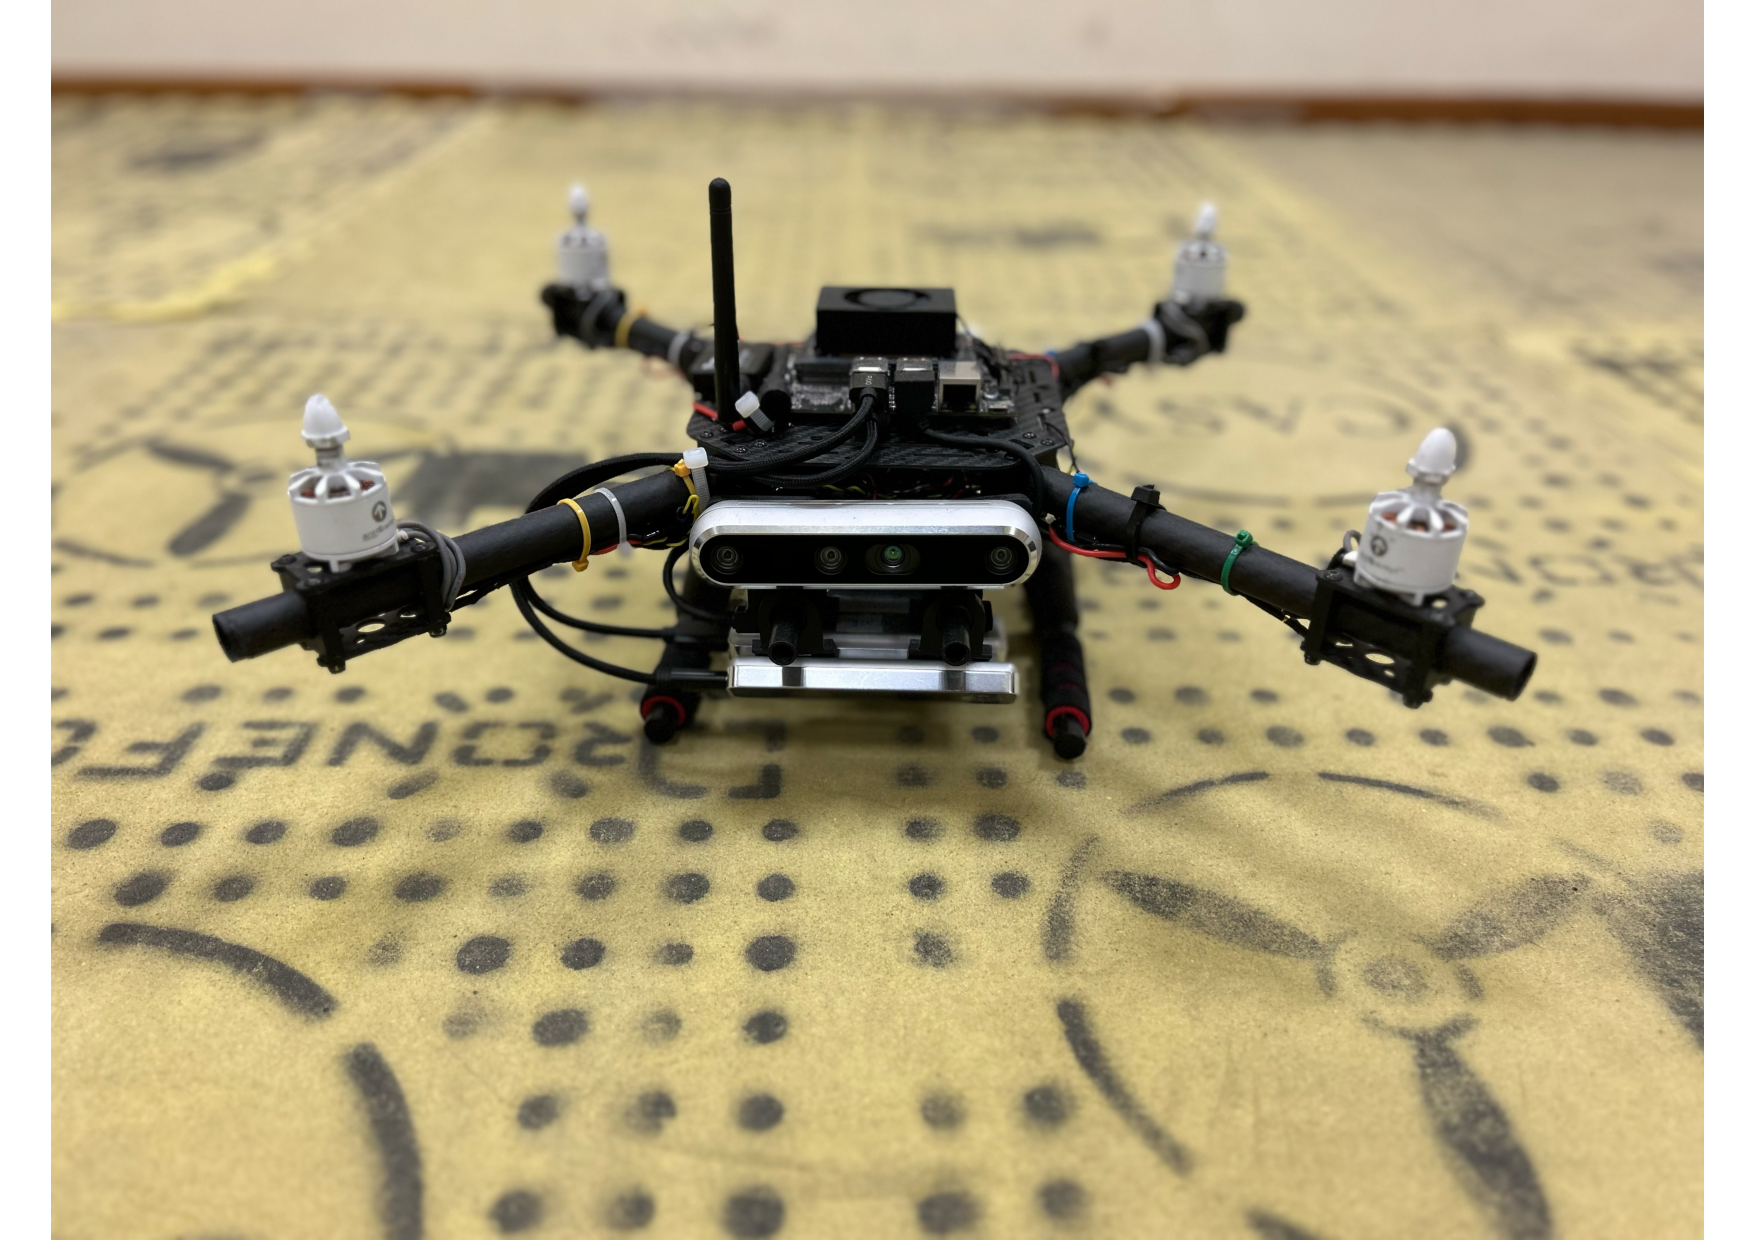
\includegraphics[width=0.8\textwidth]{Figs/Chapter1/drone.pdf}
	\caption{Developed drone used during the Leonardo drone contest.}
	\label{FIG:DRONE-PLATFORM}
\end{figure}
%%%%%%%%%%
The quadcopter deployed during the Leonardo drone contest (see~\figref{FIG:DRONE-PLATFORM}) is a commercial drone 
\emph{Holybro X500} customized for our particular application, of dimension $750 \times 750 \times 370$ millimeters,
with a weight of $1530$ grams, and is powered with a $6200$ \emph{mAh} battery. The quadcopter is endowed with a
\emph{Pixhawk 4}~\cite{meier2011pixhawk} computational unit running the \emph{PX4 Autopilot}~\cite{meier2015px4}.
Besides this unit, the UAV carries a \emph{Jetson Xavier NX} companion computer responsible for running all
control, planning, localisation, and perception algorithms. All the developed algorithms are tightly integrated
inside a ROS network and exchange messages with the Pixhawk computational unit via \emph{MAVLink} interface~\cite{koubaa2019micro}.
The chosen sensor suite consists of a $9$-axis Inertial Measurement Unit (IMU), inclusive of accelerometers, gyroscopes, and
magnetometers, and two stereo cameras pointing backward and forward, respectively.
The sensor suite is intentionally poor and GPS free, to let the robot navigate in GPS-denied environments such as indoor areas,
and to keep the overall platform cost low.
The overall quadcopter comprising of all sensors and computational units weights $1960$ grams and has a payload of $500$ grams
at $60\%$ of throttle.

%----------------------------------------------------------------------------------------
\section{Contributions}%
\label{SEC:CONTRIBUTIONS}
The contribution of this thesis is twofold, on one side it is meant to present and describe a practical software solution
to the problem of autonomous navigation in unknown, or partially known, environments.
Such a solution has been extensively tested and validated in real scenario experiments and presented as a final UAV architecture
during the Leonardo drone contest (see~\secref{SEC:DRONE-CONTEST}).
The proposed solution is often built upon existing stat-of-the-art algorithms properly modified and robustified to cope with
the strong real-time and reliability requirements imposed by the contest.
A reader only interested in the aforementioned architecture hardly finds a smooth discussion of all software modules.
The thesis presentation is in fact intentionally left unstructured, although the chapters sequence remark the
localisation-planning-control pipeline, each chapter decomposes the problem at hand and in addition to providing a
practical solution, it aspires to present innovative ideas and contributions.
This is the second contribution of this thesis that, for each aspect of autonomous navigation, tries to improve
the current state-of-the-art by leveraging on solutions which reduce, or eliminate, the major limitations of the
most popular algorithms.

%------------------------------------------------
\chapter{Quadrotor Modeling and Control}%
\label{CH:MODELING-AND-CONTROL}

In this chapter we briefly collect and review the ``golden standards'' in quadcopter modeling and control, borrowing the formalism and the
results from~\cite{tal2020accurate, faessler2017differential, kai2017nonlinear, mellinger2011minimum, richter2016polynomial, sun2022comparative, falanga2018pampc}.
The chapter unfolds as follows, in~\secref{SEC:QUADROTOR-MODELING} we develop the quadrotor dynamical model, in~\secref{SEC:DIFFERENTIAL-FLATNESS}
we describe a very useful property of the developed model known as \emph{differential flatness}.
Then in~\secref{SEC:QUADROTOR-CONTROL} %and~\secref{SEC:TRAJECTORY-GENERATION}
we briefly describe two possible quadcopter control approaches.
%and how the reference trajectories can be generated.
This chapter is intentionally poor in terms of scientific contribution as it is meant to introduce the reader to the complex world
of quadcopter motion planning and control.

%----------------------------------------------------------------------------------------
\section{Quadrotor Modeling}%
\label{SEC:QUADROTOR-MODELING}
Let $\II = \{ e^{\II}_1, e^{\II}_2, e^{\II}_3 \}$ denotes a right-hand inertial frame stationary with respect to the earth and
such that $e^{\II}_3$ denotes the vertical direction downwards into the earth.
Let the vector $\bs{\xi} = \lp x, y, z \rp\T \in \R^3$ denotes the position of the centre of mass of the object in the frame $\II$
relative to a fixed origin $O_{\II} \in \R^3$. Let $\BB = \{ e^{\BB}_1, e^{\BB}_2, e^{\BB}_3 \}$ be a body-fixed reference frame
whose center coincides with the center of mass of the vehicle and such that $e^{\BB}_3$ is in the opposite direction of thrust generation.
The attitude of the body-fixed frame is represented by a rotation matrix $R \in SO(3) : \BB \mapsto \II$, with $SO(3)$ the Special Orthogonal
group of dimension $3$.
Applying the Newton-Euler equations to the system, it is possible to retrieve the translational and rotational kinematics
\begin{equation}%
\label{EQ:QUADROTOR-KINEMATICS}
    \begin{split}
        \dot{\bs{\xi}} & = \bs{v}, \\
        \dot{R} & = RS\lp \bs{\omega} \rp,
    \end{split}
\end{equation}
with $\bs{\omega} \in \R^3$ and $\bs{v} \in \R^3$ denoting the vector of coordinates of the angular velocity and the linear 
vehicle velocity with respect to $\II$, while $S\lp \bs{\omega} \rp$ denotes the skew-symmetric matrix associated with the
vector $\bs{\omega}$, and the translational and rotational dynamics
\begin{equation}%
\label{EQ:QUADROTOR-DYNAMICS}
    \begin{split}
        \dot{\bs{v}} & = m^{-1}fRe^{\II}_3 - ge^{\II}_3, \\
        \dot{\bs{\omega}} & = -S(\bs{\omega})\bs{\omega} + J^{-1}\bs{\tau},
    \end{split}
\end{equation}
with $m \in \R$ and $J \in \R^{3 \times 3}$ being the quadrotor mass and inertia matrix with respect to the frame $\BB$,
$g \in \R$ the gravity acceleration, $f \in \R$ the collective thrust generated by the four rotors, and $\bs{\tau} \in \R^3$
the torque vector expressed in the frame $\BB$.
The system inputs are the collective thrust $f$ and the torque vector $\bs{\tau}$ which are directly generated by the rotation
of the four rotors. In particular, each rotor has an angular speed $\omega_i$ and produces a force, $F_i$, and moment, $M_i$, according to
\begin{equation*}
    F_i = k_F \omega^2_i, \hspace{0.5cm} M_i = k_M \omega^2_i,
\end{equation*}
therefore the control input to the system can be expressed as
\begin{equation*}
    \begin{pmatrix}
        f \\ \tau_x \\ \tau_y \\ \tau_z
    \end{pmatrix} =
    \begin{pmatrix}
        k_F & k_F & k_F & k_F \\
        0 & k_FL & 0 & -k_FL \\
        -k_FL & 0 & k_FL & 0 \\
        k_M & -k_M & k_M & -k_M
    \end{pmatrix}
    \begin{pmatrix}
        \omega_1^2 \\ \omega_2^2 \\ \omega_3^2 \\ \omega_4^2
    \end{pmatrix},
\end{equation*}
with $L \in \R$ the distance from the axis of rotation of the rotors to the center of the quadrotor.
For further details about the modeling of the constants $k_F \in \R$ and $k_M \in \R$ the reader is referred to~\cite{kai2017nonlinear}.
Equations~\eqref{EQ:QUADROTOR-KINEMATICS} and~\eqref{EQ:QUADROTOR-DYNAMICS} express the system dynamics with the aid of the rotational
matrix $R$, the same equation can be equivalently expressed using the quaternion dynamics as
\begin{equation}%
    \label{EQ:QUATERNION-QUADROTOR-DYNAMICS}
    \begin{split}
        \dot{\bs{\xi}} & = \bs{v}, \\
        \dot{\bs{q}} & = 0.5 \Lambda(\bs{\omega})\bs{q}, \\
        \dot{\bs{v}} & = m^{-1}fR(\bs{q})e^{\II}_3 - ge^{\II}_3, \\
        \dot{\bs{\omega}} & = -S(\bs{\omega})\bs{\omega} + J^{-1}\bs{\tau},
    \end{split}
\end{equation}
with
\begin{equation*}
    R(\bs{q}) =
    \begin{pmatrix}
        1 - 2(q_y^2 + q_z^2) & 2(q_x q_y - q_z q_w) & 2(q_x q_z + q_y q_w) \\
        2(q_x q_y + q_z q_w) & 1 - 2(q_x^2 + q_z^2) & 2(q_y q_z - q_x q_w) \\
        2(q_x q_z - q_y q_w) & 2(q_y q_z + q_x q_w) & 1 - 2(q_x^2 + q_y^2)
    \end{pmatrix},
\end{equation*}
and the matrix $\Lambda \in \R^{4 \times 4}$ defined as
\begin{equation*}
    \Lambda(\bs{\omega}) = \begin{pmatrix}
        0 & -\omega_x & -\omega_y & -\omega_z \\
        \omega_x & 0 & \omega_z & -\omega_y \\
        \omega_y & -\omega_z & 0 & \omega_x \\
        \omega_z & \omega_y & -\omega_x & 0
    \end{pmatrix}.
\end{equation*}
In the aforementioned relation $\bs{q} \in \mathbb{H}$ is the normed quaternion attitude vector.
Overall the state of the system is given by the position and velocity of the center of mass and the orientation
(locally parameterized by Euler angles) and the angular velocity
\begin{equation*}
    \bs{\xx} = \lp x, y, z, v_x, v_y, v_z, \phi, \theta, \psi, \omega_x, \omega_y, \omega_z \rp\T.
\end{equation*}

%----------------------------------------------------------------------------------------
\section{Differential Flatness}%
\label{SEC:DIFFERENTIAL-FLATNESS}
In this section we recall the results of~\cite{mellinger2011minimum} showing that the quadrotor dynamics~\eqref{EQ:QUADROTOR-KINEMATICS}-\eqref{EQ:QUADROTOR-DYNAMICS}
is differentially flat~\cite{van1998real}, i.e. the states and the inputs can be written as algebraic functions of four carefully selected
flat outputs and their derivatives. This is a fundamental result as it can ease a lot the process of trajectory generation and 
optimisation, since any smooth trajectory (with reasonably bounded derivatives) in the space of flat outputs can be followed by
the underactuated quadrotor. Let $\flatoutput = \lp x, y, z, \psi \rp\T$ the selected set of flat outputs, with
$\bs{\xi} = \lp x, y, z \rp\T$ coordinates of the center of mass in the world coordinate system and with $\psi$ the yaw angle,
and define $\flatoutput(t)$ as a smooth curve in the space of flat outputs
\begin{equation*}
    \flatoutput(t) : \lps 0, T_F \rps \mapsto \R^3 \times SO(2),
\end{equation*}
then the objective is to show that the state of the system and its control inputs can be rewritten in terms of $\sigma(t)$ and its derivatives.
First of all, the position and velocity of the center of mass are simply the first three terms of $\flatoutput$ and $\dot{\flatoutput}$.
In order to reconstruct $R$ as a function of the selected flat outputs, let us define it as $R =\ ^{\II}R_{\CC}\ ^{\CC}R_{\BB}$
where $^{\II}R_{\CC}$ represents the yaw rotation to the intermediate frame $\CC$ and $^{\CC}R_{\BB}$ represents the effect of roll and pitch.
In this setting, considering~\eqqref{EQ:QUADROTOR-DYNAMICS}, we can write
\begin{equation}%
    \label{EQ:FLAT-THRUST}
    e_3^{\BB} = \frac{m}{f} \lp \ddot{\flatoutput}_x, \ddot{\flatoutput}_y, \ddot{\flatoutput}_z + g \rp,
\end{equation}
which defines the body frame $z$-axis of the quadrotor.
From the yaw angle, $\flatoutput_4 = \psi$, we can derive the unit vector
\begin{equation*}
    e_1^{\CC} = \lp \sin\lp \flatoutput_4 \rp, \cos\lp \flatoutput_4 \rp, 0 \rp\T,
\end{equation*}
while $e_1^{\BB}$ and $e_2^{\BB}$ can be determined as
\begin{equation*}
    e_2^{\BB} = \frac{e_3^{\BB} \times e_1^{\CC}}{\norm{e_3^{\BB} \times e_1^{\CC}}}, \hspace{0.5cm} e_1^{\BB} = e_2^{\BB} \times e_3^{\BB},
\end{equation*}
provided that $e_3^{\BB} \times e_1^{\CC} \ne 0$.
Finally, the rotational matrix $R$ is uniquely determined as
\begin{equation*}
    R = \lp e_1^{\BB}, e_2^{\BB}, e_3^{\BB} \rp.
\end{equation*}
Now, take the first derivative of~\eqqref{EQ:QUADROTOR-DYNAMICS}
\begin{equation*}
    \ddot{\bs{v}} = m^{-1} \lp \dot{f}e_3^{\BB} + \bs{\omega} \times f e_3^{\BB} \rp,
\end{equation*}
projecting this equation along $e_3^{\BB}$ and using the fact that $\dot{f} = e_3^{\BB} \cdot m\ddot{\bs{v}}$,
we can define the vector $\bs{h} \in \R^3$ as
\begin{equation*}
    \bs{h} = \bs{\omega} \times e_3^{\BB} = \frac{m}{f} \lp \ddot{\bs{v}} - \lp e_3^{\BB} \cdot \ddot{\bs{v}} \rp e_3^{\BB} \rp.
\end{equation*}
In this settings, $\bs{h}$ is the projection of $\frac{m}{f} \ddot{\bs{v}}$ along the $e_1^{\BB}-e_2^{\BB}$ plane.
Thus, decoposing $\bs{\omega}$ into its components $\bs{\omega} = pe_1^{\BB} + qe_2^{\BB} + re_3^{\BB}$, we can write
\begin{equation*}
    \begin{split}
        p & = - \bs{h} \cdot e_2^{\BB}, \\
        q & = \bs{h} \cdot e_1^{\BB}, \\
        r & = \dot{\flatoutput}_4 e_3^{\II} \cdot e_3^{\BB}.
    \end{split}
\end{equation*}
Finally, the components of the angular acceleration $\bs{\alpha}$ are found by computing the second of derivative of~\eqqref{EQ:QUADROTOR-DYNAMICS}
and following the same procedure as above.
Having $\flatoutput$, $\bs{\omega}$, and $\bs{\alpha}$ at hand we can exploit~\eqqref{EQ:QUADROTOR-DYNAMICS} and~\eqqref{EQ:FLAT-THRUST}
to directly compute the inputs $f$ and $\bs{\tau}$.

%----------------------------------------------------------------------------------------
\section{Quadrotor Control}%
\label{SEC:QUADROTOR-CONTROL}
The literature is cluttered with works about the stabilisation and control of aerial vehicles such as quadcopters.
In the first stage, given the unstable nature of the quadrotors, the initial works were focused on achieving stable hovering and
near-hover flights. Thanks to the small-angle assumptions in these conditions, linear control methods such as PID and LQR
demonstrate sufficiently good performance~\cite{khatoon2014pid, dong2013modeling}.
However, as increased the necessity to push these platforms toward the boundaries of their dynamical capabilities, 
these assumptions were no longer valid. In particular, the nonlinearities coming from the attitude dynamics were no longer negligible,
for this reason researchers started developing controllers based on feedback linearization~\cite{voos2009nonlinear},
backstepping~\cite{madani2006backstepping}, and geometric properties~\cite{lee2010geometric}.
Once the differential flatness property has been revealed~\cite{mellinger2011minimum}, the differential flatness-based
controller becomes the most used regulator for trajectory tracking, as it showed the best tracking performance at
relatively high speeds~\cite{faessler2017differential, tal2020accurate}.
Besides that, recently, some studies started using Model Predictive Controls (MPCs), jointly with the full quadrotor dynamics,
to compute optimal control inputs able to both stabilise the quadcopter flight and track a given reference
trajectory~\cite{bicego2020nonlinear, foehn2021time, torrente2021data}.
These methods either directly use the optimized single rotor thrust commands~\cite{bicego2020nonlinear}
or send intermediate states from the solution (such as the angular rates) to a low-level controller~\cite{foehn2021time, torrente2021data}.
A recent study~\cite{foehn2021time} demonstrates the ability of the full-model MPC with a PID low-level controller in tracking a
pre-planned race trajectory at speed up $20 m/s$ which surpasses the top speed of $12.9 m/s$ reported in~\cite{tal2020accurate} using
a differential flatness-based controller, in spite of a much larger tracking error.

In this chapter, we briefly review these two main used control techniques based on the flatness property explained in~\secref{SEC:DIFFERENTIAL-FLATNESS}
and on the MPC tool. In the particular case of the Leonardo drone contest, we employed a non-linear model predictive controller encoding
the full quadrotor dynamics~\eqref{EQ:QUATERNION-QUADROTOR-DYNAMICS}.  

\subsection{Differential Flatness-Based Controller}
Let define the errors on position and velocity as
\begin{equation*}
    \bs{\ee}_{\bs{\xi}} = \bs{\xi} - \bs{\xi}_{\text{ref}}, \hspace{0.5cm} \bs{\ee}_{\bs{v}} = \bs{v} - \bs{v}_{\text{ref}},
\end{equation*}
then the desired force vector is
\begin{equation*}
    F_{\text{des}} = - K_{\bs{\xi}} \bs{\ee}_{\bs{\xi}} - K_{\bs{v}} \bs{\ee}_{\bs{v}} + mg e_3^{\II} + m\dot{\bs{v}}_{\text{ref}},
\end{equation*}
where $K_{\bs{\xi}}$ and $K_{\bs{v}}$ are positive definite gain matrices.
In order to compute the desired force for the quadrotor, that correspond to the first input $f$, we simply project the desired
force vector onto the actual body frame $z$-axis
\begin{equation*}
    f = F_{\text{des}} \cdot e_3^{\BB}.
\end{equation*}
To determine the other three inputs, we must consider the rotation errors.
First, observe that the desired $e_3^{\BB}$ direction is along the desired thrust vector
\begin{equation*}
    e_{3_{\text{des}}}^{\BB} = \frac{F_{\text{des}}}{\norm{F_{\text{des}}}},
\end{equation*}
thus the desired rotation is given by
\begin{equation*}
    R_{\text{des}} e_3 = e_{3_{\text{des}}}^{\BB},
\end{equation*}
with $e_3 = \lp 0, 0, 1\rp\T$.
Knowing the specified yaw angle along the trajectory, $\psi(t)$, we can compute $e_{1_{\text{des}}}^{\BB}$ and
$e_{2_{\text{des}}}^{\BB}$ as
\begin{equation*}
    e_{1_{\text{des}}}^{\CC} = \lp \cos\lp \psi \rp, \sin\lp \psi \rp, 0 \rp\T,
\end{equation*}
and 
\begin{equation*}
    e_{2_{\text{des}}}^{\BB} = \frac{e_{3_{\text{des}}}^{\BB} \times e_{1_{\text{des}}}^{\CC}}{\norm{e_{3_{\text{des}}}^{\BB} \times e_{1_{\text{des}}}^{\CC}}},
    \hspace{0.5cm} e_{1_{\text{des}}}^{\BB} = e_{2_{\text{des}}}^{\BB} \times e_{3_{\text{des}}}^{\BB}.
\end{equation*}
provided that $e_{3_{\text{des}}}^{\BB} \times e_{1_{\text{des}}}^{\CC} \ne 0$.
Next, define the error in orientation
\begin{equation*}
    \bs{\ee}_{R} = 0.5 \lp R_{\text{des}}\T R - R\T R_{\text{des}} \rp^{\land},
\end{equation*}
where $R_{\text{des}} = \lp e_{1_{\text{des}}}^{\BB}, e_{2_{\text{des}}}^{\BB}, e_{3_{\text{des}}}^{\BB}\rp$ and $^{\land}$
represents the \emph{vee map} which takes elements of $so(3)$ to $\R^3$.
The angular velocity error is simply the difference between the actual and desired angular velocity in body frame
\begin{equation*}
    \bs{\ee}_{\bs{\omega}} = \bs{\omega} - \bs{\omega}_{\text{ref}},
\end{equation*}
then the desired moments can be computed as
\begin{equation*}
    \bs{\tau} = -K_R \bs{\ee}_R -K_{\bs{\omega}} \bs{\ee}_{\bs{\omega}},
\end{equation*}
where $K_R$ and $K_{\bs{\omega}}$ are diagonal gain matrices.

\subsection{Nonlinear Model Predictive Controller}
Model predictive control generates control commands by solving a finite-time Optimal Control Problem (OCP)
in a receding horizon fashion. Given a reference trajectory, the cost function is the error between the predicted states
and the reference states inside the time horizon, meaning that multiple reference points in the time horizon are used.
In order to perform numerical optimizations, we discretize the states and inputs into $N$ equal intervals over
the time horizon $\rho \in \lps t, t+h\rps$ of size $\Delta_t = h/N$ with $h$ denoting the horizon length,
yielding a constrained nonlinear optimization problem
\begin{equation*}
    \begin{split}
        \bs{\uu} = \arg \min_{\bs{\uu}} & \sum_{k=0}^{N-1} \lp \norm{\bs{\xx}_k - \bs{\xx}_{k, \text{ref}}}_{Q} + 
                                                         \norm{\bs{\uu}_k - \bs{\uu}_{k, \text{ref}}}_{R}\rp +
                                                         \norm{\bs{\xx}_N - \bs{\xx}_{N, \text{ref}}}_{Q_N}\\
        & 
        \begin{split}
        sub. to. \hspace{0.2cm} & \bs{\xx}_{k+1} = \xfun \lp \bs{\xx}_k, \bs{\uu}_k \rp, \\
        & \bs{\xx}_0 = \bs{\xx}_{\text{init}}, \\
        & \bs{\uu} \in \lps \bs{\uu}_{\text{min}}, \bs{\uu}_{\text{max}} \rps, \\ 
        & \bs{\omega} \in \lps \bs{\omega}_{\text{min}}, \bs{\omega}_{\text{max}} \rps,
        \end{split}
    \end{split}
\end{equation*}
where the state vector is defined as $\bs{\xx} = \lp \bs{\xi}\T, \bs{v}\T, \bs{q}\T, \bs{\omega}\T \rp\T$, the input
vector as $\bs{\uu} = \lp f, \bs{\tau}\T \rp\T$, and $Q$, $R$, and $Q_N$ are positive definite matrices that shape as
\begin{equation*}
    Q = \text{diag} \lp Q_{\bs{\xi}}, Q_{\bs{v}}, Q_{\bs{q}}, Q_{\bs{\omega}} \rp, \hspace{0.2cm}
    R = \text{diag} \lp Q_{f}, Q_{\bs{\tau}} \rp, \hspace{0.2cm}
    Q_N = Q.
\end{equation*}
The reference state vector $\bs{\xx}_{\text{ref}}$ and input $\bs{\uu}_{\text{ref}}$ can be obtained from a trajectory generator procedure as described in the next chaptes,
while the function $f \lp \bs{\xx}_k, \bs{\uu}_k \rp$ is the discretized version of the full nonlinear quadrotor model~\eqref{EQ:QUATERNION-QUADROTOR-DYNAMICS}.
\begin{remark}
    In the above optimization problem, the following abuse of notation is used when calculating quaternion error
    \begin{equation*}
        \bs{q} - \bs{q}_{\text{ref}} = \bs{q} \otimes \bs{q}_{\text{ref}}^{-1}
    \end{equation*}
\end{remark}
The above MPC solves the full nonlinear model of a quadrotor, instead of resorting to a cascaded structure, or linear assumptions.
The solution presented during the Leonardo drone contest resorts on this control thecnique, where the quadratic nonlinear optimization problem is solved
by a Sequential Quadratic Programming (SQP) algorithm executed in real-time.
The algorithm has been implemented using ACADO~\cite{verschueren2018towards} toolkit with qpOASES~\cite{ferreau2014qpoases} as solver.

%----------------------------------------------------------------------------------------
% \section{Trajectory Generation}%
% \label{SEC:TRAJECTORY-GENERATION}

%% TODO: Add GP-MPC Applied to Rover
% \section{Data-Driven Model Predictive Control}
% %%%%%%%%%%
% \begin{figure}[!t]
% 	\centering
% 	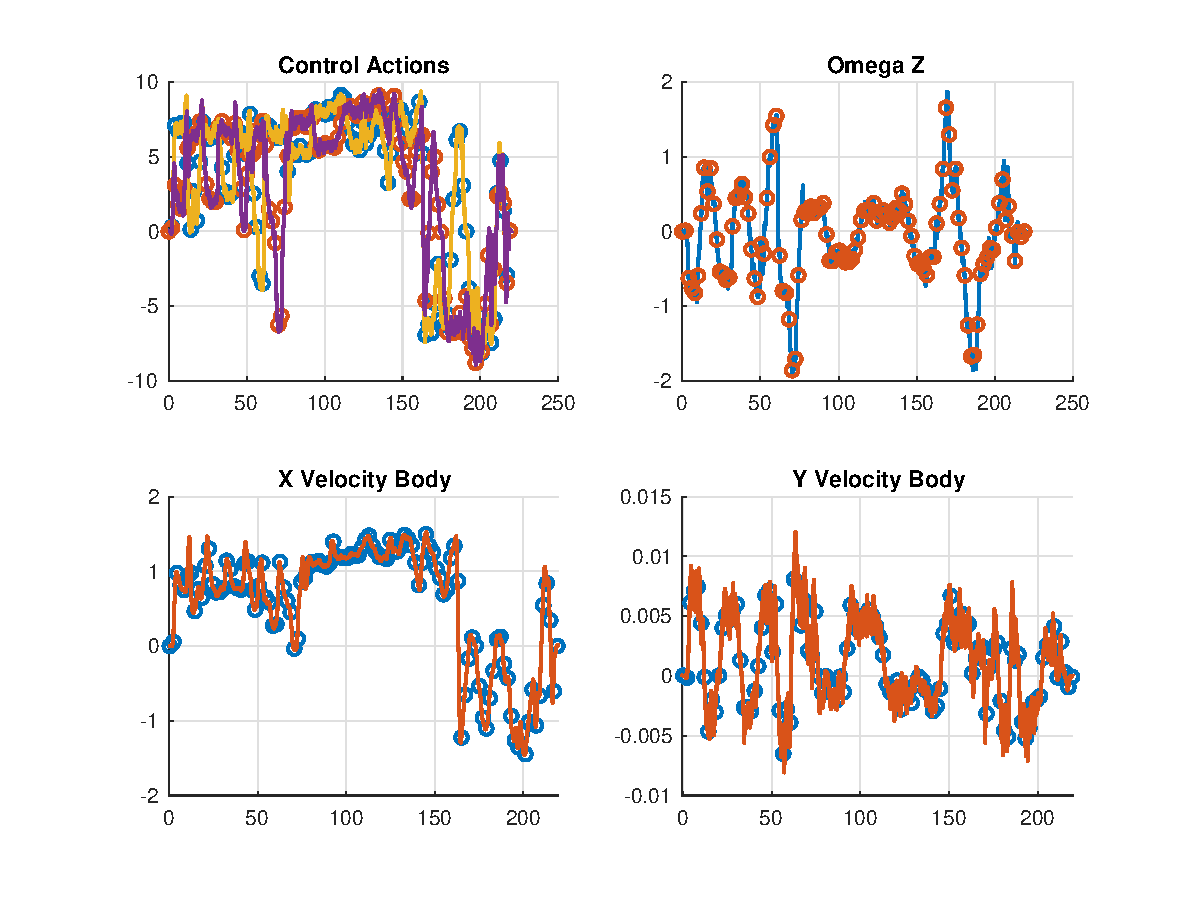
\includegraphics[width=1.\textwidth]{Figs/Chapter2/mpc_gp_sampled_quantities.eps}
% 	\caption{Caption here.}
% 	% \label{FIG:}
% \end{figure}
% %%%%%%%%%%
% %%%%%%%%%%
% \begin{figure}[!t]
% 	\centering
% 	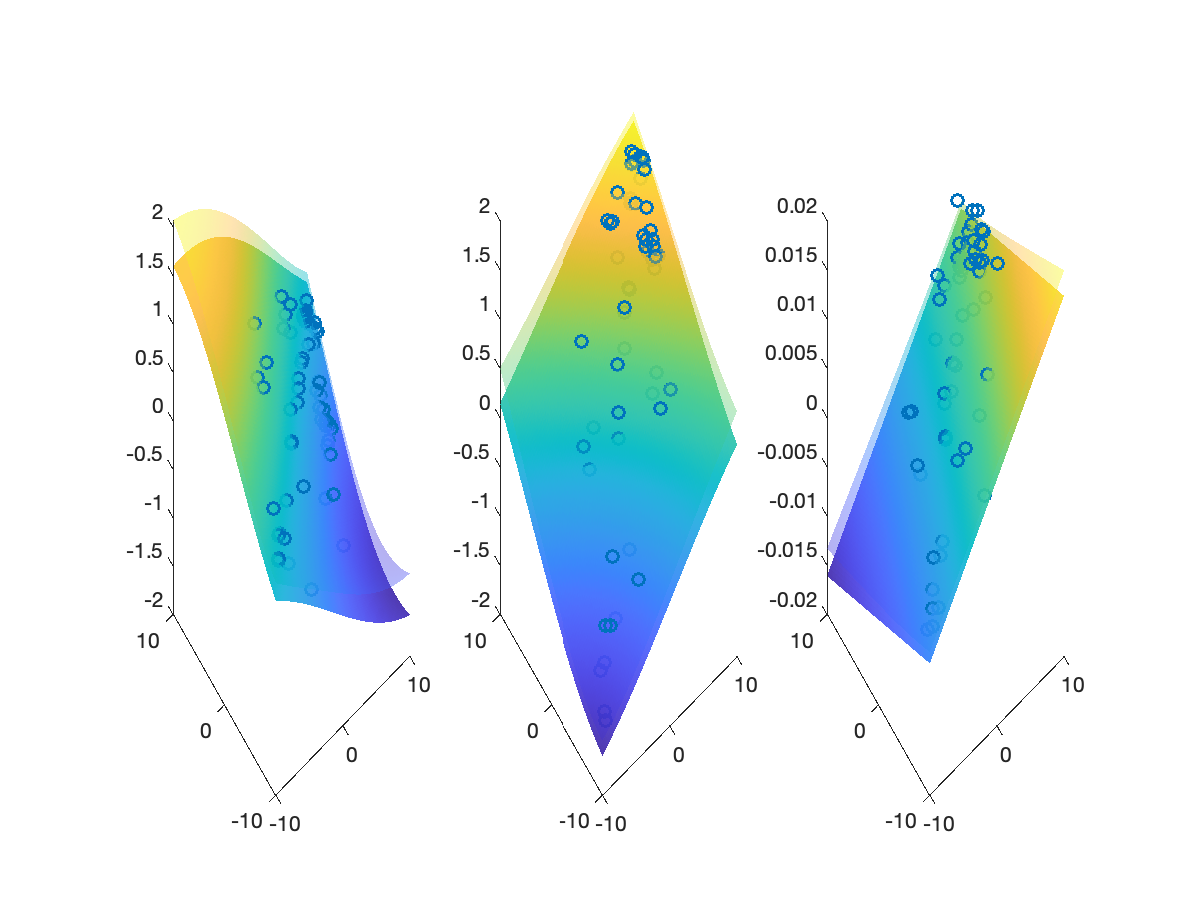
\includegraphics[width=1.\textwidth]{Figs/Chapter2/mpc_gp_regression_nl.eps}
% 	\caption{Caption here.}
% 	% \label{FIG:}
% \end{figure}
% %%%%%%%%%%
% %%%%%%%%%%
% \begin{figure}[!t]
% 	\centering
% 	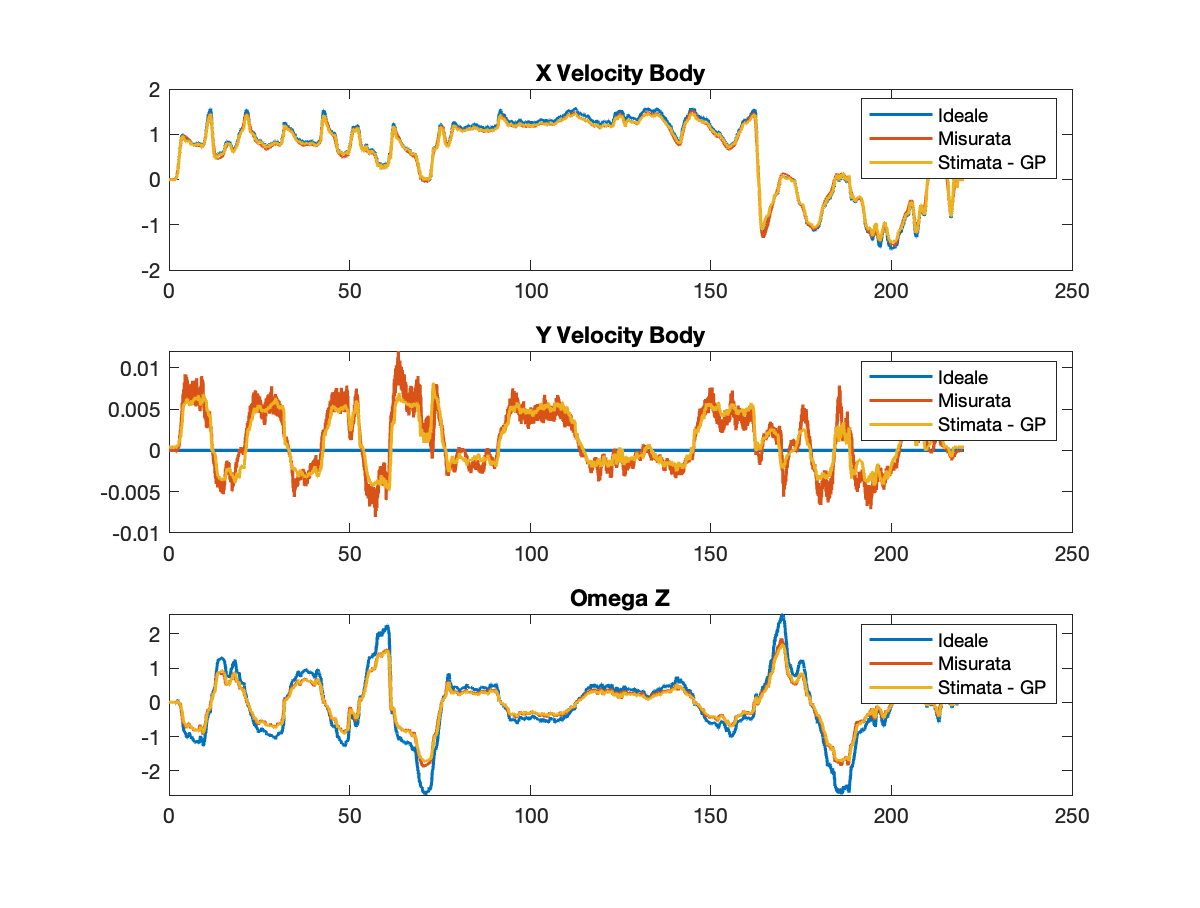
\includegraphics[width=1.\textwidth]{Figs/Chapter2/mpc_gp_test_samedata.eps}
% 	\caption{Caption here.}
% 	% \label{FIG:}
% \end{figure}
% %%%%%%%%%%
% %%%%%%%%%%
% \begin{figure}[!t]
% 	\centering
% 	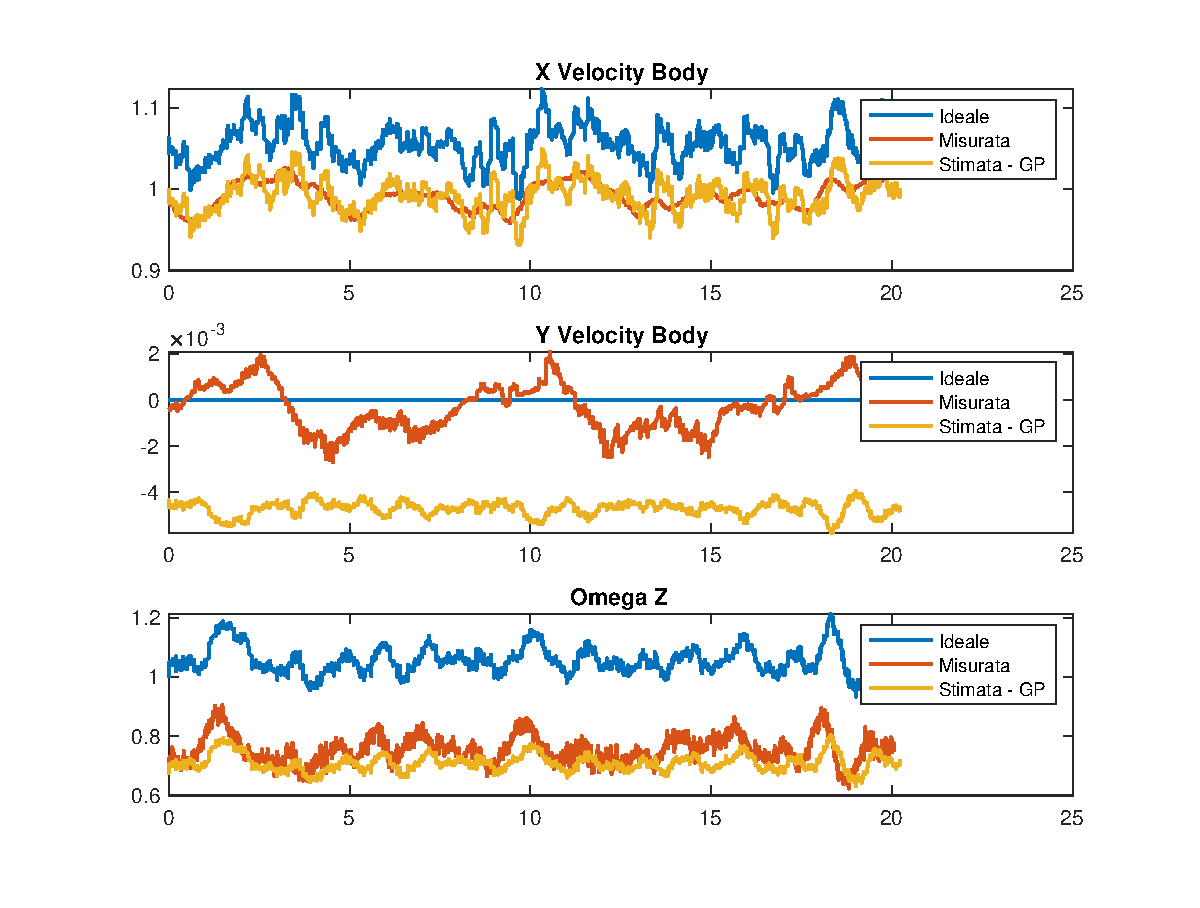
\includegraphics[width=1.\textwidth]{Figs/Chapter2/mpc_gp_test_differentdata.eps}
% 	\caption{Caption here.}
% 	% \label{FIG:}
% \end{figure}
% %%%%%%%%%%
% %%%%%%%%%%
% \begin{figure}[!t]
% 	\centering
% 	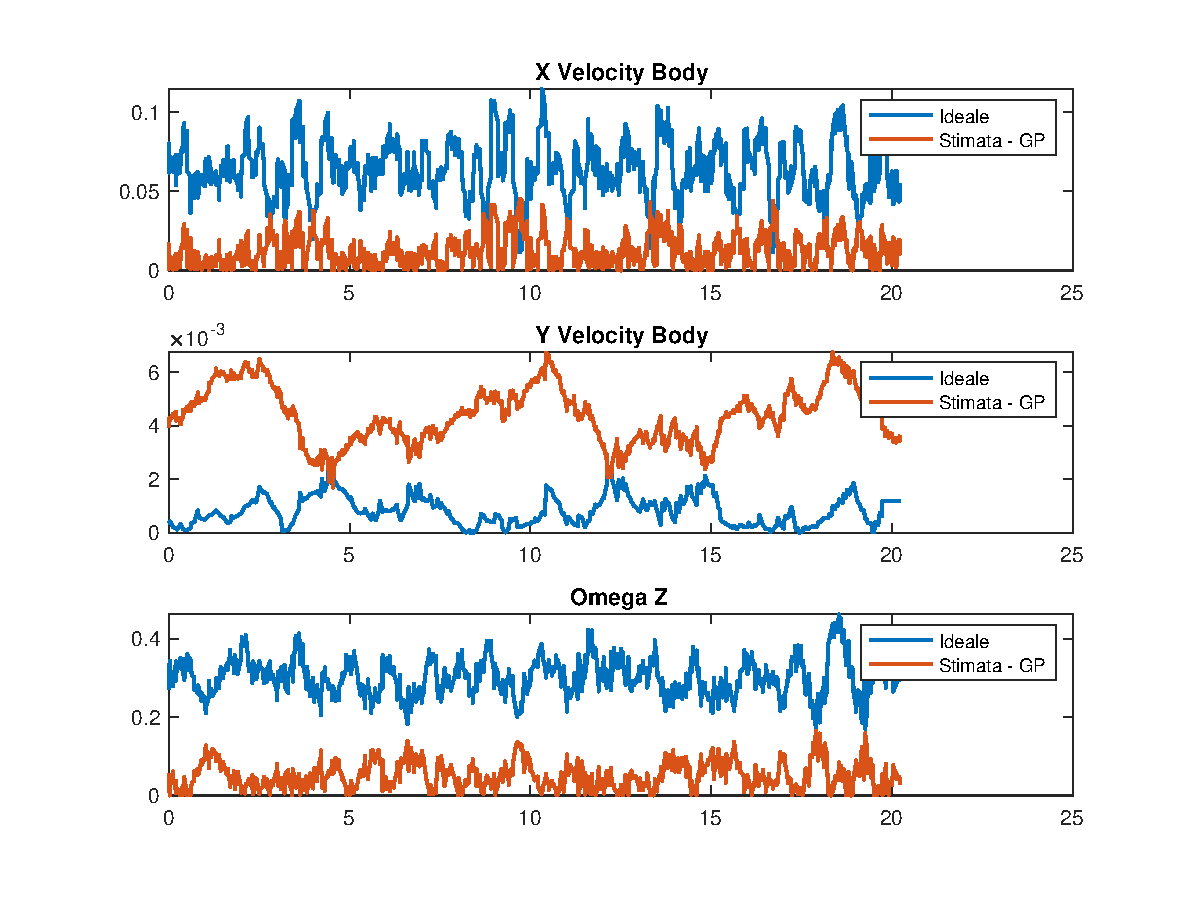
\includegraphics[width=1.\textwidth]{Figs/Chapter2/mpc_gp_test_differentdata_errors.eps}
% 	\caption{Caption here.}
% 	% \label{FIG:}
% \end{figure}
% %%%%%%%%%%

%------------------------------------------------
\cleardoublepage % Empty page before the start of the next part

%------------------------------------------------
% \ctparttext{Introduction and contribution of the planning stack.
% the use of pointers, intead of pipes, makes the overall stack very efficient.}
\part{Autonomous Motion Planning}

\chapter{Environment Mapping and Localisation}%
\label{CH:MAPPING}

%----------------------------------------------------------------------------------------
\section{The Framework}%
\label{SEC:MANDL-FRAMEWORK}
The problem of Simultaneous Localisation And Mapping (SLAM) is related to the issue of concurrently estimating the robot position, in a
\emph{local} or \emph{global} reference system, and mapping the obstacles, or visual clues, present in the environment under exploration.
SLAM is the process by which a robot builds a map of the environment and, at the same time, uses this map to compute its location,
as the reader can conceive such a problem undergoes the so-called \emph{chicken-egg} dilemma as a map is needed to perform localisation,
but a pose estimation is necessary to build the map. To enable planning and navigation a reliable and resilient localisation is of fundamental
importance as it can provide the reference systems necessary to ground the onboard drone intelligence.
Such a problem has been widely studied and a large number of solutions have been presented along
the literature, for a large number of different sensors, starting from frame monocular~\cite{forster2014svo, mur2015orb, qin2018vins} and
stereo cameras~\cite{gomez2019pl, mur2017orb, campos2021orb}, to event cameras~\cite{vidal2018ultimate},
and LiDAR sensors~\cite{zhang2014loam, xu2021fast, xu2022fast, kim2021scan, caballero2021dll}.
In the specific case of the Leonardo drone contest (see~\secref{SEC:DRONE-CONTEST}), the autonomous robot was required to perform SLAM with some apriori information at hand,
as the environment under exploration was already mapped by means of user-friendly tools, and a three-dimensional geometrical reconstruction was
made available for the robot. In these settings, the only way to localise inside the precomputed environment reconstruction was to exploit the
endowed stereo camera to build a local pointcloud, via stereo matching, and match it with the provided 3D map, in a purely LiDAR SLAM
paradigm~\cite{zhang2014loam, xu2021fast, xu2022fast, kim2021scan, caballero2021dll}.
At the same time, visual SLAM approaches, as well as the build pointcloud, could have been used to enrich the initial map with new
details useful to improve the localisation stability.
Following the latter intuition, we choose to deploy two different SLAM solutions working in parallel on two different sets of data.
On one side, we employ state-of-the-art visual-inertial-based SLAM approaches to estimate the robot motion with respect to an \emph{odometry}
frame~\cite{mur2015orb, qin2018vins}, by means of hardware-calibrated stereo images, while, on the other hand, we borrow from the LiDAR
SLAM field the idea of pointcloud matching to precisely align the sensed pointcloud with the apriori provided map.

In this chapter we review and adapt a novel pointcloud matching algorithm, designed for LiDAR-based localisation, to the case of
quadrotor localisation in cluttered environments using limited FoV sensors, such as stereo cameras.
For further details the reader is referred to the original work~\cite{caballero2021dll}.

\subsection{Related Works}
The literature is cluttered with works trying to solve both the problems of LiDAR odometry and SLAM, although
very few of them deeply discuss the problem of map-based localisation, considering it a sub-class of problem strictly related to the SLAM one.
A recent comprehensive review of LiDAR-based localisation solutions for ground vehicles can be found in~\cite{elhousni2020survey}.
The basic idea, on which most of the solutions are grounded, is to register (aka match) the current LiDAR reading into a local submap, being it
composed by the last LiDAR measure or a collection of data from previously registered points.
As the reader can conceive, matching every point of the LiDAR data with every point of the current map is a process that quickly grows and reaches
infeasibility due to the limited computation capabilities available, especially onboard drones.
To overtake this limitation, most state-of-the-art solutions make use of geometric features such as corners or planes directly extracted from the sensors
pointcloud~\cite{zhang2014loam, liu2019precise, choy2019fully}.
The key idea is to select points or areas that are easy to identify and match when reviewed again from a different perspective, point of view, or distance.
LOAM~\cite{zhang2014loam} exploits exactly this idea, as it extracts point features on sharp edges and planar surfaces and matches them between consecutive scans.
On the other hand~\cite{dube2018incremental} uses a similar approach, pointcloud segments and descriptors are used to perform localisation;
while MULLS~\cite{pan2021mulls} tries to increase the localisation accuracy by combining a feature-based front-end SLAM with a multi-cetric ICP for map alignment.
Although feature-based LiDAR-to-map registration approaches show very good results with low computational burden, they may fail in poor texture scenes, or
when multiple occlusions happen.
Iterative Closest Points (ICP)-based approaches~\cite{chen1992object} showed better performance and robustness with respect to the aforementioned issues,
as their use the raw pointcloud for registration, and no features or interest points are extracted.
This accuracy and stability come at the price of a high computational burden, especially when dealing with large pointcloud maps.
Moreover, the ICP convergence strongly depends on the quality of the provided initial pose estimation.
In the literature can be found a bunch of works aiming to approximate the neighbors search procedure~\cite{muja2009fast, elseberg2012comparison}, which turns out
to be the major computational bottleneck. While many ICP variants have been proposed to improve the 
global robustness against noise or bad initialization by means of new criteria as Branch-and-Bound in GO-ICP~\cite{yang2015go},
or reformulating the ICP problem as Expectation-Maximization in EM-ICP~\cite{granger2002multi},
or as a Truncated Lest Squares in TEASER~\cite{yang2020teaser}.
The Normal Distribution Transform (NDT) was the first approach to propose nearest-neighbor-free solution for pointcloud registration~\cite{magnusson2007scan, hong2017probabilistic}
allowing for very high accuracy while avoiding the computational burden induced by ICP approaches.
The NDT is used to encode both scan and map using a probabilistic representation.
Registration is then performed between these representations and not the original scans.
Such a representation allows for numerical optimization methods, and does not require expensive nearest-neighbor search procedures.
Recently,~\cite{caballero2021dll} proposed a direct approach for registration, where the raw pointcloud is registered inside the map
in a nearest-neighbor-free fashion. The registration is reformulated as a non-linear least square optimisation problem which aims to
minimise the scan points distance to the current environment map continuously maintained as a Euclidean Signed Distance Field (ESDF).

%----------------------------------------------------------------------------------------
\section{An Optimization-based Localization Approach}
\subsection{Problem Formulation}
Let $\MM = \{ e^{\MM}_1, e^{\MM}_2, e^{\MM}_3 \}$ denotes a right-hand inertial frame associated with the provided three-dimensional reconstruction,
and let $\SF = \{ e^{\SF}_1, e^{\SF}_2, e^{\SF}_3 \}$ be a sensor-fixed reference frame, rigidly attached to the body-fixed one $\BB$
by means of a static transformation $^{\BB}T_{\SF} = \lps ^{\BB}R_{\SF}, \{\bs{t}_{\SF}\}_{\BB} \rps \in SE(3)$, with $SE(3)$ the Special Euclidean group
of dimension $3$. Assume that the endowed sensor, being a stereo-frame camera in the Leonardo drone contest case, streams as output a pointcloud
$\{\PC^k\}_{\SF} = \{ \{\bs{p}^k_0\}_{\SF}, \{\bs{p}^k_1\}_{\SF}, \dots, \{\bs{p}^k_{N_p^k}\}_{\SF} \}$ at each timestamp $k \in \R_{\ge 0}$, consisting of
$N_p^k$ points $\{\bs{p}^k_i\}_{\SF} \in \R^{3}$ expressing the obstacles position in the sensor reference frame $\SF$.
Moreover, assume that a map of the environment is also available as a pointcloud $\{\PC^k\}_{\MM} = \{ \{\bs{p}^k_0\}_{\MM},
\{\bs{p}^k_1 \}_{\MM}, \dots, \{\bs{p}^k_{N_m^k} \}_{\MM} \}$, where each point $\{\bs{p}^k_i \}_{\MM}$ is static inside the interval $\lps k, k+1 \rps$.
In this setting, the localisation goal is to find the transformation $^{\MM}T_{\SF} = \lps ^{\MM}R_{\SF}, \{\bs{t}_{\SF}\}_{\MM} \rps \in SE(3)$
that better aligns $\{\PC^k\}_{\SF}$ with $\{\PC^k\}_{\MM}$. In other terms, the goal is to find out the minimiser of the optimisation problem
\begin{equation}
    \label{EQ:LOCALISATION-OPTIMISATION-COMPLEX}
    \argmin_{^{\MM}T_{\SF}} \sum_{i = 0}^{N_p^k} \norm{^{\MM}T_{\SF} \{\bs{p}^k_i\}_{\SF} - 
                            \argmin_{\{\bs{p}^k \}_{\MM}} \norm{^{\MM}T_{\SF} \{\bs{p}^k_i\}_{\SF} - \{\bs{p}^k_j \}_{\MM}}^2}^2,
\end{equation}
where 
\begin{equation*}
    \argmin_{\{\bs{p}^k \}_{\MM}} \norm{^{\MM}T_{\SF} \{\bs{p}^k_i\}_{\SF} - \{\bs{p}^k_j \}_{\MM}}^2
\end{equation*}
represents the \emph{map} point closest to $^{\MM}T_{\SF} \{\bs{p}^k_i\}_{\SF}$.
Solving the aforementioned problem needs to deal with two major challenges, first how to determine the closest map point, and
then how to solve a massively overdetermined non-linear optimization problem.
ICP solutions work by iteratively searching for pairs of nearby points in the two pointclouds and minimising the sum of all
point-to-point distances, while NDT approaches model the pointclouds as combinations of normal distributions instead of individual points,
describing the probability of finding a point at a certain position. The latter piecewise smooth representation allows for standard numerical optimisation methods for registration.
Since the major bottleneck in registration is represeted by the nearest neighbor search, NDT solutions generally work better, with high performance.
For this reason,~\cite{caballero2021dll} follows the same NDT idea, and converts the registration process in a non-linear optimization problem where
pointclouds are modeled as Euclidean distance fields. Let $d^k\lp \bs{p} \rp : \R^3 \mapsto \R$ be the ESDF build up with the map points
$\{\PC^k\}_{\MM}$ at time $k$, then~\eqref{EQ:LOCALISATION-OPTIMISATION-COMPLEX} boils down to
\begin{equation}
    \label{EQ:LOCALISATION-OPTIMISATION-SIMPLE}
    \argmin_{^{\MM}T_{\SF}} \sum_{i = 0}^{N_p^k} d^k \lp ^{\MM}T_{\SF} \{\bs{p}^k_i\}_{\SF} \rp^2.
\end{equation}
The map $d^k\lp \bs{p} \rp$ is everywhere continuous and smooth, except to the object boundaries where the gradient is discontinuous~\cite{jones20063d},
so the aforementioned optimisation problem can be solved using off-the-shelf non-linear least squares solvers (eg. Ceres~\cite{agarwal2022ceres}).
\begin{remark}
    Due to the high nonlinearities encoded in~\eqref{EQ:LOCALISATION-OPTIMISATION-SIMPLE}, its convergence to the global optimum is ensured only in front of
    good enough initial conditions. To overtake this problem, a state-of-the-art visual-inertial-based SLAM approach has been employed to
    estimate the robot motion between two different time instants $k$ and $k+1$, in order to supply~\eqref{EQ:LOCALISATION-OPTIMISATION-SIMPLE}
    with a very good initial condition.
\end{remark}
\begin{remark}
    When dealing with~\eqref{EQ:LOCALISATION-OPTIMISATION-SIMPLE}, it is of fundamental importance to keep care about possible outliers.
    In particular, the sensed pointcloud may contain objects not mapped yet, such as dynamic obstacles that can cross the environment, or
    previously unmapped static obstacles, or may contain points that fall outside the map bounds.
    At the same time, the sensed pointcloud may be affected by noise and can contain many points that do not belong to any object in the scene.
    To overtake these problems three actions have been taken to improve the solver convergence
    \begin{enumerate}
        \item The sensed pointcloud is pre-elaborated with a bunch of downsampling and outliers removal filters.
        \item A robust Cauchy kernel is applied to each loss factor in~\eqref{EQ:LOCALISATION-OPTIMISATION-SIMPLE}, in order to penalize large costs
              induced by outliers and not matched points (in the nearest neighbor sense).
        \item If a point lies outside the map, the ESDF returns a zero value, producing both error and gradient equal to zero to avoid affecting the optimization process.
    \end{enumerate}
\end{remark}

\subsection{Signed Distance Field Computation}
As emerges from the previous section,~\cite{caballero2021dll} encodes the ESDF inside the optimisation problem~\eqref{EQ:LOCALISATION-OPTIMISATION-COMPLEX}
in place of the nearest neighbor search, to speed-up its solution.
This choice has the advantage to avoid heavy nearest neighbor searches, at the expense of ESDF computation, which can turn out to be
very computationally expensive for large environments. As a matter of fact,~\cite{caballero2021dll} proposes to build-up the Euclidean field
offline, and assume the environment to be static, so the precomputed map is always valid.
Such an assumption is clearly not satisfied in the Leonardo drone contest settings (\secref{SEC:DRONE-CONTEST}), thus we require to build and
adapt the signed distance online to account for environments modifications.
Although along the literature there exist several different approaches to compute ESDFs, both in
discrete~\cite{oleynikova2017voxblox, han2019fiesta}, and continuous settings~\cite{popovic2017multiresolution, stork2020ensemble, wu2021faithful},
none of these is able to cope with prior map information, so we propose a novel structured approach able to account for previous maps
and to locally modify the computed ESDF to cope with environment modifications.
Unlike state-of-the-art approaches, our method assumes a bounded map and is able to add and remove newly sensed obstacles, but is unable
to remove previously already mapped objects.

The proposed ESDF computation follows two steps.
In the first offline stage it builds up the distance field of the apriori mapped environment, to do so the overall environment is
discretised with a fixed resolution $\Delta = \lps \Delta_x, \Delta_y, \Delta_z \rps$, then each cell grid $\bs{\xi}_i \in \R^3$
is filled with the squared distance of the closest map point $\{\bs{p}^0 \}_{\MM}$
\begin{equation*}
    \min_{\{\bs{p}^0 \}_{\MM}} \norm{\bs{\xi}_i - \{\bs{p}^0_j \}_{\MM}}^2.
\end{equation*}
The latter nearest neighbor search is performed via FLANN KDTree search~\cite{muja2009flann}.
\begin{remark}
    The built FLANN KDTree is kept maintained in memory and used later for ESDF online adaptation.
\end{remark}
The second step is performed online, at each new sensor update, the incoming cloud $\{\PC^k\}_{\SF}$ is downsampled and
filtered against possible outliers, then it is converted in map coordinate via the estimated transformation $^{\MM}T_{\SF}$
and inserted inside an octree probability occupancy map~\cite{hornung2013octomap}, build-up with the same discretisation resolution $\Delta$.
The latter insertion is fundamental to robustify the approach both in terms of sensor noise and possible localisation errors.
All previously free cell grids branded as \emph{occupied}, and all previously occupied cells branded as \emph{free} are grouped into
two vectors and used for the distance field update.
\begin{itemize}
    \item[] \emph{From free to occupied.} \\
    A new (very small) FLANN KDTree is build out of the provided point vector, then each ESDF cell grid is updated with the minimum
    between the current cell value and the distance computed over the last built KDTree.
    \item[] \emph{From occupied to free.} \\
    Two new (very small) FLANN KDTrees are build out of the provided point vector, and the current occupied voxels from the occupancy map.
    Then each ESDF cell grid is updated with the minimum between the original map distance and the one evaluated on the occupancy map KDTree,
    only if the current cell value matches with the distance evaluated on the point vector KDTree. 
\end{itemize}
The first step explains the insertion procedure, which turns out to be very easy, as each cell grid is replaced with the new minimum 
distance, while the second step analyzes the removal procedure.
In the latter step, the point vector KDTree is used to identify each map cell affected by the removal, then it is updated with the minimum
between the original map distance and the distance evaluated on the new sensed obstacles.
\begin{remark}
    Due to the discrete nature of the adopted ESDF, the map $d^k\lp \bs{p} \rp$ presents discontinuities at the cell borders, losing the
    required smoothness to let~\eqref{EQ:LOCALISATION-OPTIMISATION-SIMPLE} converge properly.
    To overtake this limitation we approximate the real value of $d^k\lp \bs{p} \rp$ via trilinear interpolation.
\end{remark}
\begin{remark}
    The overall approach can be speeded-up by restricting the occupancy points insertion to only those that do not belong to previously mapped obstacles
    (i.e. belong to new scene objects).
\end{remark}
\begin{remark}
    The proposed approach is not able to deal with the removal of previously mapped obstacles that have been moved, leaving the previously occupied
    space free. This represents a strong limitation in the case of high dynamic scene, where obstacles may continuously change their location, but
    on the other hand, this assumption leads to a conservative solution suitable for our case of study.
\end{remark}

%----------------------------------------------------------------------------------------
\section{Contributions}
This chapter is devoted to discuss the problem of localisation and mapping in dynamic scenarios where some apriori information,
in the format of three-dimensional geometrical reconstruction, of the navigating environment was provided.
The discussion unfolds by first reviewing the current state-of-the-art solutions both in terms of SLAM, occupancy mapping, and ESDF reconstruction,
then we propose the adaptation of the most promising solution, to the quadcopter navigation case, where stereo-frame cameras are used to 
retrieve a pointcloud reconstruction of the surroundings. The selected solution is then extended to dynamic environment scenarios via
a novel structured approach to continuously update the computed ESDF. The proposed solution has the limitation of obstacle removal, as it
is not able to remove objects scene already mapped inside the initial geometrical reconstruction.
The proposed localisation approach has been successfully developed and deployed inside the Leonardo drone contest.

%------------------------------------------------
\chapter{Environment Exploration}%
\label{CH:EXPLORATION}

%----------------------------------------------------------------------------------------
\section{The Framework}%
\label{SEC:EXPLORATION-FRAMEWORK}
The ability to autonomously plan and execute informative trajectories in previously unknown, or partially known,
environments is a fundamental requirement for mobile robots. As a matter of fact, they started to be employed
in a huge number of different applications which require the ability to efficiently collect new information
about the surroundings, such as surface inspection, object search, weed recognition, search and rescue missions, and others.
The problem of Informative Path Planning (IPP), jointly with the problem of environment exploration, has been extensively
studied in literature and a wide variety of approaches have been proposed so far. The majority of recent works had
focused on novel hybrid approaches leveraging the interplay between the concepts of \emph{local} and \emph{global}
exploration~\cite{selin2019efficient,schmid2020efficient}. In particular, the major issue behind such works is related
to how efficiently combine the two local and global exploration steps, and how to plan highly informative global
paths out of the current environment information. A limited number of papers focused on improving the local exploration
step~\cite{selin2019efficient}. On the other hand, the necessity to push the autonomous platform always toward unknown
frontiers limited the research of solutions where the environment is a priori known, or partially known, and the agent
should perform patrolling-like operations~\cite{dang2018autonomous}. In this chapter, we present two novel approaches
aiming, in the first stage, to push the current state-of-the-art toward more smooth and resilient solutions for local
exploration in cluttered and possibly varying environments, and, in the second stage, to adapt global exploration tools
to the problem of fast environment patrolling and object search.

\subsection{Related Works}%
\label{SEC:EXPLORATION-RELATED-WORKS}
Although the number of solutions presented in the literature is quite variegated, the majority of them can be classified as
\emph{frontier-based} or \emph{sampling-based} methods. The former class was pioneered in~\cite{yamauchi1997frontier} and
later more comprehensively developed in~\cite{julia2012comparison}. The key idea is to guide the agent toward the borders
between free and unmapped space (aka frontiers), since these points may represent those with higher potential information gain.
Exploration is then carried out by extracting the map frontiers and by navigating through them sequentially.
Several works propose to extend it by adding constraints to ensure low localization errors~\cite{stachniss2005information}.
The basic frontier-based approach has been also extended to high-speed flight for fast exploration in~\cite{cieslewski2017rapid}.
In this case, the authors propose to extract frontiers only inside the current Field-Of-View (FoV) and select the one leading
to the minimal change in velocity. In recent years, other works focused on rapid exploration~\cite{zhou2021fuel}, by planning
global coverage paths and optimising them with respect to the robot dynamics, and on the reformulation of the frontier information
gain as a differentiable function~\cite{deng2020robotic}, allowing paths to be optimised with gradient information. On the other hand,
\emph{sampling-based} methods typically sample random viewpoints to explore the space in a Next-Best-View (NBV)
fashion~\cite{connolly1985determination, maver1993occlusions}. Much of the work in this domain can be traced back
to~\cite{gonzalez2002navigation}, where the NBV problem has been moved for the first time from the computer graphic field to the
robotic domain, with the introduction of the notion of reconstruction gain. The concept of NBV exploration has been afterward extended
by~\cite{bircher2016receding}, where the building of a Rapidly-Exploring Random Tree (RRT) allows one to weigh both the amount of
information gained at the viewpoints and during the agent motion to reach each viewpoint. Unlike frontier-based methods, which
are difficult to adapt to other tasks, the sampling-based ones have the advantage to allow any kind of gain formulation.
Thanks to that, the original NBV algorithm was extended to consider the uncertainty of localisation~\cite{papachristos2017uncertainty, tovar2006planning}
and the visual importance of different objects~\cite{dang2018visual}. On the other hand, sampling-based methods suffer from stacking
in local minima, leading to a premature ending of the exploration procedure in unlucky scenarios. For this reason, the recent trend is
to merge the two frontiers and sampling-based approaches in a local-global exploration fashion. The pioneer of this idea
was~\cite{charrow2015information}, which makes use of a frontier method to detect global goals and supplements these with motion primitives
for local exploration. More recent approaches, instead, leverage the capabilities of sampling-based methods and employ additional planning
stages to escape from local minima~\cite{selin2019efficient,dang2019graph}. Other approaches focus on memorising previously visited places
and sampled information under the format of roadmaps~\cite{witting2018history, xu2021autonomous}. Similarly, the work presented
in~\cite{schmid2020efficient} continuously maintains and expands a single RRT of candidate paths. Although the literature has seen some
impressive works in the field of NBV, there are very few works concentrating on fast exploration. Even if previous solutions are able to
quickly plan global coverage paths~\cite{schmid2020efficient, xu2021autonomous, kompis2021informed}, the problem of efficient trajectory
planning is rarely addressed. Both under the perspective of local exploration and the patrolling, or object finding, problem.

\subsection{Problem Definition}%
\label{SEC:EXPLORATION-PROBLEM-DEFINITION}
The problem addressed in this chapter consists of exploring, as fast as possible, a bounded 3D volume $\V \subset \R^3$.
Each point $ \xx = \lp x, y, z \rp \in \V$ of this space can take only two values, i.e. \emph{free} or \emph{occupied},
and  the problem of exploration ideally consists of clustering the volume $\V$ in the free
$\V_{\text{free}} = \{ \xx \in \V \mid \Gamma(\xx) = \text{free} \}$ or occupied
$\V_{\text{occ}} = \{ \xx \in \V \mid \Gamma(\xx) = \text{occ} \}$ volumes, with a mapping function
$\Gamma(\xx): \V \mapsto \left\{ \text{free}, \text{occ} \right\}$.
Since this operation is subjected to the agent constraints and its sensing capabilities, it may happen that some map point
cannot be observed by construction. These points will remain unmapped and, for this reason, we introduce a further set
$\V_{\text{res}}$ collecting the residual points that cannot be observed. Thus, the exploration will be considered complete
when $\V_{\text{free}} \cup \V_{\text{occ}} = \V \setminus \V_{\text{res}}$. Due to the nature of the problem, it has to be
solved in real-time by planning suitable safe trajectories through the free space which is not known a priori.

%----------------------------------------------------------------------------------------
\section{Large-Scale Environments Exploration}%
\label{SEC:EXPLORATION-LARGE-SCALE}
In this section, we propose a novel solution to the aforementioned exploration problem (\secref{SEC:EXPLORATION-PROBLEM-DEFINITION})
in a setting where timing is the major issue during the task of completely unknown environment exploration. The basic idea behind the
proposed solution is that efficient local procedures allow for a very high speed up in the overall task. Although the global-local
paradigm is fundamental to ensure consistency and completeness of the exploration procedure, it is not the key to compute efficient 
exploration paths, due to the fact that the switching between local and global may lead to a waste of time, requiring the agent 
to change direction very frequently. On the other hand, optimising local trajectories with respect to the agent capabilities and
the locally gathered information of the environment under exploration may lead to faster motions, low energy consumption, and lower
waste of time. This is especially true when dealing with Unmanned Aerial Vehicles (UAVs), whose high maneuverability motivates solutions
able to stress the quadrotor to fully exploit both its computational and dynamical capabilities.
Similarly to~\cite{selin2019efficient} and~\cite{bircher2016receding}, the core of the proposed solution consists of an RRT-inspired~\cite{lavalle1998rapidly}
sampling-based exploration algorithm that aims to directly plan highly informative feasible trajectories in known space, leading to an
optimal local exploration procedure. The obtained tree is executed one node at a time, in a receding-horizon fashion.
Unlike previous works, our algorithm employs a B\acuteacc ezier curve parameterisation to grow and maintain a tree of possible trajectory
segments. The proposed approach weights both potential information gain and trajectory cost during the selection of the next goal.
Moreover, the planned trajectory does not constrain the end velocity to zero, thus the exploration can be performed quickly
by avoiding ``stop-and-go'' like behaviors. Motivated by the promising results obtained using hybrid approaches~\cite{selin2019efficient},
we allow adaptability of the proposed solution by letting the tree be easily extended with global exploration routines.
In particular, we implemented efficient rewiring procedures in order to keep in memory and continuously refine the same tree, following
the ideas of roadmaps memorisation~\cite{xu2021autonomous} and continuous tree expansion~\cite{schmid2020efficient}.
We show that the combination of the planning of both path and the associated timing law leads to a solution outperforming the state-of-the-art approaches
in this field, which usually plans point-to-point trajectories requiring stopping the robot at each exploration step.

\subsection{B\acuteacc ezier Trajectory Parameterisation}%
\label{SEC:EXPLORATION-TRAJECTORY-PARAMETERISATION}
In this framework, instead of using traditional polynomial functions, we adopt the Bernstein polynomial basis and define trajectories as
piecewise B\acuteacc ezier curves. A B\acuteacc ezier curve is completely defined by its degree $\order$ and a set of $\cpnumber = \order+1$
control points $\CP = \lps \bs{\cpoint}_0 \cdots \bs{\cpoint}_{\order} \rps$, with $\bs{\cpoint}_i \in \R$. The curve can be evaluated, for any
$ \splinevar \in [0, 1]$, as
\begin{equation}
	\label{EQ:BEZIER-SIMPLE}
	\bs{\spline} \lp \splinevar \rp = \sum_{i=0}^{\order} \basis_i^{\order}\lp \splinevar \rp \bs{\cpoint}_i,
\end{equation}
where the basis functions $\basis_i^{\order} \lp \splinevar \rp$ are $\order$th degree
\emph{Bernstein basis polynomials}~\cite{farouki2012bernstein, biagiotti2008trajectory} of the form
\begin{equation*}
	\basis_i^{\order}\lp \splinevar \rp = \frac{\order!}{i!(\order - i)!} \splinevar^i {(1 - \splinevar)}^{\order - i}.
\end{equation*}
A gentle introduction to B\acuteacc ezier curves can be found in~\appref{SEC:SPLINES-APPENDIX}, to seek of clarence we report here the major
properties required to properly understand the subsequent analysis. The aforementioned polynomials enjoy a partition-of-unity property
(i.e. $\sum_{i=0}^{\order} \basis_i^{\order} \lp \splinevar \rp = 1$ for all $\splinevar$), by which the curve defined by~\eqqref{EQ:BEZIER-SIMPLE}
is constrained inside the convex hull generated by its control points $\CP$. Moreover, a $\order$-degree B\acuteacc ezier curve is always
$\order$ times differentiable and its derivatives preserve a B\acuteacc ezier structure of lower degree. In particular,
$\spline' \lp \splinevar \rp := d\spline/d\splinevar$ is a B\acuteacc ezier curve of order $\order-1$ whose control points $\CP'$ can be
evaluated as $\bs{\cpoint}'_i = \order \lp \bs{\cpoint}_{i+1} - \bs{\cpoint}_i \rp$ $\forall i = 0, \dots, \order-1.$ The overall quadrotor reference
trajectory can be expressed through the evolution of its \emph{flat outputs}~\cite{mellinger2011minimum}, as explained in~\secref{SEC:DIFFERENTIAL-FLATNESS},
$\flatoutput = {\lps \rr, \yaw \rps}\T$, where $\rr = {\lps x, y, z \rps}\T \in \R^3$ represents the coordinates of the
center of mass in the world coordinate system, while $\yaw \in \R$ is the yaw angle. Both the quantities $\rr$ and $\yaw$ are expressed as
$\segnumber$-segments piecewise B\acuteacc ezier curves of order $\order_{\rr}$ and $\order_{\yaw}$, respectively
\begin{equation*}
	\rr \lp t \rp=
	\begin{cases}
		\sum_{i=0}^{\order_{\rr}} \basis_i^{\order_{\rr}}(\clock_1) \rr^1_i & \hspace{-0.2cm} t \in [T_0, T_1],\\
		\sum_{i=0}^{\order_{\rr}} \basis_i^{\order_{\rr}}(\clock_2) \rr^2_i & \hspace{-0.2cm} t \in [T_1, T_2],\\
		\hspace{0.2cm} \vdots & \vdots \\
		\sum_{i=0}^{\order_{\rr}} \basis_i^{\order_{\rr}}(\clock_{\segnumber}) \rr^{\segnumber}_i & \hspace{-0.2cm} t \in [T_{\segnumber-1}, T_{\segnumber}],\\
	\end{cases}
\end{equation*}
\begin{equation*}
	\yaw \lp t \rp=
	\begin{cases}
		\sum_{i=0}^{\order_{\yaw}} \basis_i^{\order_{\yaw}}(\clock_1) \yaw^1_i & \hspace{-0.2cm} t \in [T_0, T_1],\\
		\sum_{i=0}^{\order_{\yaw}} \basis_i^{\order_{\yaw}}(\clock_2) \yaw^2_i & \hspace{-0.2cm} t \in [T_1, T_2],\\
		\hspace{0.2cm} \vdots & \vdots \\
		\sum_{i=0}^{\order_{\yaw}} \basis_i^{\order_{\yaw}}(\clock_{\segnumber}) \yaw^{\segnumber}_i & \hspace{-0.2cm} t \in [T_{\segnumber-1}, T_{\segnumber}],\\
	\end{cases}
\end{equation*}
with $\clock_i = \frac{t-T_{i-1}}{T_{i}-T_{i-1}}$. The quantities $\rr_i^j \in \R^3$ and $\yaw_i^j \in \R$ describe the $i^{th}$ control
point of the $j^{th}$ trajectory segment of $\rr(t)$ and $\yaw(t)$ respectively, while $T_{j-1}$ and $ T_j$ are the start and end time of
the $j^{th}$ trajectory segment. Note that the introduced time scaling does not affect the spatial path described by the B\acuteacc ezier
curve, but strongly affects its derivatives as 
\begin{align*}
	{\rr'}^j_i & = \frac{\order_{\rr}(\rr^j_{i+1}-\rr^j_i)}{T_{j-1}-T_j} \hspace{0.2cm} \forall i=0,\dots,\order_{\rr}-1 , \\
	{\yaw'}^j_i & = \frac{\order_{\yaw}(\yaw^j_{i+1}-\yaw^j_i)}{T_{j-1}-T_j} \hspace{0.2cm} \forall i=0,\dots,\order_{\yaw}-1 .
\end{align*}
\begin{figure}[!t]
	\begin{minipage}{.45\linewidth}
		\centering
		\subfloat[]{%
			\label{FIG:EXPLORATION-BEZIER-CURVE-A}%
			\includegraphics[scale=.85]{Figs/Chapter4/bezier_conservative.pdf}}
	\end{minipage}
	\begin{minipage}{.45\linewidth}
		\centering
		\subfloat[]{%
			\label{FIG:EXPLORATION-BEZIER-CURVE-B}%
			\includegraphics[scale=.85]{Figs/Chapter4/bezier_envelope.pdf}}
	\end{minipage}
	\caption{Representation of a fifth-degree B\acuteacc ezier curve with
	(a) the classical sphere used for collision checking~\cite{tang2020real}
	(b) the proposed multiple spheres envelope.
	The $\mathcal{O}$ shaded gray area represents a generic obstacle.}\label{fig:BEZIER-CURVE}
\end{figure}
The \emph{convex hull containment} property is a powerful tool to verify both the trajectory feasibility in terms of dynamic constraints,
such as velocity or acceleration bounds, and to check for collisions. \figref{FIG:EXPLORATION-BEZIER-CURVE-A} reports the classical
condition used for collision checking with B\acuteacc ezier curves~\cite{tang2020real}, where the overall curve is constrained inside a
\emph{safe} sphere. The aforementioned approach often results in being too conservative, as a matter of fact the considered sphere
is far to be tight over the convex hull, and thus over the curve itself. For this reason we formulate a new proposition that represents
a less conservative tool to verify collision (see \figref{FIG:EXPLORATION-BEZIER-CURVE-B}).
\begin{proposition}%
	\label{PROPOSITION:EXPLORATION-ENVELOPE-CONTAINMENT}
	Let $\rr \lp \splinevar \rp$ be a B\acuteacc ezier curve of order $\order$, with control points $\CP= \lps \rr_0, \dots, \rr_{\order} \rps$.
	Moreover, let $\ri_i \in \R$  and $\cc_i \in \R^3$ with $i=0, \dots, \order$ be respectively the radii and centre of $\order$ spheres
	($\mathcal{C}_0 \dots \mathcal{C}_{\order}$), defined as:
	\begin{equation*}
		\begin{split}
			\cc_i & = (\rr_i + \cc)/2, \\
			\ri_i & = \norm{\rr_i - \cc_i},
		\end{split}
	\end{equation*}
	with $\cc$ be the centre of the convex hull generated by $\CP$, i.e. $\cc = \sum_{i=0}^{\order} \rr_i/\order$.
	Then the curve $\rr \lp \splinevar \rp$ is entirely contained inside the spheres envelope, namely
	\begin{equation*}
		\rr \lp \splinevar \rp \in \bigcup_{i=1}^{\order} \mathcal{C}_i \hspace{0.5cm} \forall \splinevar \in [0,1].
	\end{equation*}
\end{proposition}
\begin{proof}
    The proof follows from the fact that $\cc$ belongs to the convex hull and that the spheres envelope composed by
	$\mathcal{C}_i$ and $\mathcal{C}_{i+1}$ always contains the convex hull edge $\overline{\rr_i\rr_{i+1}}$.
	The first statement is true by construction, since $\cc$ is a linear combination of $\rr_i$, while the second one
	follows from the triangle inequality
	\begin{equation*}
		\norm{\rr_i - \rr_{i+1}} \le \norm{\rr_i - \cc} + \norm{\rr_{i+1} - \cc}. \qedhere
	\end{equation*} 
\end{proof}
\propref{PROPOSITION:EXPLORATION-ENVELOPE-CONTAINMENT} states that the convex hull containment property can be reformulated taking
into account a set of $\order$ spheres. Since this set of spheres results to be tighter around the curve with respect to a single big
safe ball, the use of this proposition in formulating a new collision condition results in a less conservative approach.
The following proposition states the sufficient condition for non-collision as a corollary of~\propref{PROPOSITION:EXPLORATION-ENVELOPE-CONTAINMENT}.
\begin{proposition}%
	\label{PROPOSITION:EXPLORATION-COLLISION-FREE}
	Let $\rr \lp \splinevar \rp$ be a B\acuteacc ezier curve of order $\order$, with control points $\CP= \lps \rr_0, \dots, \rr_{\order} \rps$.
	Moreover, let $\cc_i$ and $\ri_i$ with $i=0,\dots,\order$ be the centre and radii of $\order$ spheres defined as
	in~\propref{PROPOSITION:EXPLORATION-ENVELOPE-CONTAINMENT}. The curve $\rr \lp \splinevar \rp$ is said to be collision-free,
	with a safety bound of $d^{\text{safe}} \in \R_{+}$, if the condition
	\begin{equation*}
		\ri_i - d^{\text{obs}}_{\cc_i} - d^{\text{safe}} > 0 \hspace*{0.5cm} \forall i = 0, \dots, \order
	\end{equation*}
	holds, where $d^{\text{obs}}_{\cc_i}$ represents the Euclidean distance of $\cc_i$ from the closest obstacle.
\end{proposition}
From now on, we use fifth-order B\acuteacc ezier curves to represent the quadrotor position ($\order_{\rr} = 5$),
while the yaw trajectory is parameterised using third-order B\acuteacc ezier curves ($\order_{\yaw} = 3$).

\subsection{Tree Structure}%
\label{SEC:EXPLORATION-TREE-STRUCTURE}
The proposed algorithm works by growing and maintaining, at each iteration, a tree $\tree = \lp \nodes, \edges \rp$ of possible trajectories.
Such tree consists of a set of nodes $\nodes = \{\node_1, \dots, \node_{\dd{\node}}\}$ and a set of edges
$\edges = \{\edge_i, \dots , \edge_{\dd{\edge}}\}$. Each node $\node_i$ is completely defined by the following five quantities
\begin{equation*}
	\node_i = \left\{ g_i, c_i, \delta_i, \CP^{\rr}_i, \CP^{\yaw}_i \right\}
\end{equation*}
where $g_i = g \lp \node_i \rp$ represents the amount of information gained if that node is executed, and $c_i = c \lp \node_i \rp$
is the cost associated to the node execution. $\CP^{\rr}_i$ and $\CP^{\yaw}_i$ are the two sets of control points defining the
trajectories $\rr_i(t)$ and $\yaw_i(t)$, while $\delta_i$ is the execution time. Two nodes $\node_{i-1}$ and $\node_{i}$ are connected
by an edge $\edge_{i-1}$ only if the first $(\order_{\rr/\yaw}+1)/2$ control points of the latter node satisfy some continuity criterion with
the last $(\order_{\rr/\yaw}+1)/2$ control points of the former one. This constraint is required to ensure continuity among all trajectory
segments of the tree. In particular, since $\order_{\rr} = 5$ and $\order_{\yaw} = 3$, we enforce continuity up to the third derivative along
$\rr(t)$ and continuity up to the second derivative along $\yaw(t)$, namely
\begin{align}
	\label{EQ:EXPLORATION-FIRST-COND}
	&\rr^{i}_0  = \rr^{i-1}_5,\\
	\label{EQ:EXPLORATION-SECOND-COND}
	&\frac{1}{\delta_{i}}(\rr^{i}_1 - \rr^{i}_0)  = \frac{1}{\delta_{i-1}}(\rr^{i-1}_5 - \rr^{i-1}_4),\\
	\label{EQ:EXPLORATION-THIRD-COND}
	&\frac{1}{\delta_{i}^2}(\rr^{i}_2 - 2\rr^{i}_1 + \rr^{i}_0)  = \frac{1}{\delta_{i-1}^2}(\rr^{i-1}_5 - 2\rr^{i-1}_4 + \rr^{i-1}_3),\\
	\label{EQ:EXPLORATION-FOURTH-COND}
	&\yaw^{i}_0  = \yaw^{i-1}_3,\\
	\label{EQ:EXPLORATION-FIFTH-COND}
	&\frac{1}{\delta_{i}}(\yaw^{i}_1 - \yaw^{i}_0)  = \frac{1}{\delta_{i-1}}(\yaw^{i-1}_3 - \yaw^{i-1}_2).
\end{align}
The aim is to plan sub-optimal trajectories by maximising a user-specified utility function $\loss \lp \RR \lp \node_i \rp \rp$,
with $\RR \lp \node_i \rp$ be the sequence of nodes connecting $\node_i$ to the tree root, which properly combines gains and costs
of all nodes in $\RR \lp \node_i \rp$. In this context, the tree root is defined as the tree node which is about to be executed by the
flying agent. It results that the agent behavior strongly depends on the choice of functions $g \lp \node_i \rp$, $c \lp \node_i \rp$
and $\loss \lp \RR \lp \node_i \rp \rp$. The proposed algorithm is agnostic with respect to these functions. Therefore, the user can specify
any formulation of them by ensuring that the following criteria are satisfied~\cite{schmid2020efficient}:
\begin{enumerate}
	\item $g \lp \node_i \rp$ should be a function that depends on the trajectory end position only ($g \lp \rr^i_5, \yaw^i_3 \rp$),
	\item all node gains should be mutually independent,
	\item $c \lp \node_i \rp$ is required to be an intrinsic property of the trajectory ($c\lp\CP^{\rr}_i, \CP^{\yaw}_i, \delta_i\rp$).
\end{enumerate}

\subsection{Tree Update}%
\label{SEC:EXPLORATION-TREE-UPDATE}
The tree, initially composed by just one root node, is iteratively expanded by randomly sampling viewpoints inside a sphere centred on
the current \emph{best node} ($\node_{\text{best}}$), namely the one among all tree nodes that maximise the utility function $\loss(\cdot)$.
In particular, the sphere is centred exactly on the last control point of $\CP^{\rr}_{\text{best}}$, i.e. $\rr^{\text{best}}_5$, while
its radius ($r_{\text{sp}}$) is a user chosen value defined as a parameter for the algorithm. The sampled viewpoint is retained only if
it belongs to a known and free part of the environment under exploration and, at the same time, it is far enough from the mapped obstacles.
Such viewpoint is considered as the last control point of the next trajectory segment ($\rr^{i}_5$). Moreover, due to
Condition~\eqref{EQ:EXPLORATION-FIRST-COND}, also the control point $\rr^{i}_0$ is already defined to ensure position continuity.
As regards the heading trajectory, the first control point ($\yaw^i_0$) is established through Condition~\eqref{EQ:EXPLORATION-FOURTH-COND},
while the last one ($\yaw^i_3$) is chosen as the value that maximise the potential information gain $g(\rr_5^i, \yaw)$, namely
\begin{equation*}
	\yaw_i^3 = \arg \max_{\yaw} \ g(\rr_5^i, \yaw),
\end{equation*}
in a similar way as done in~\cite{selin2019efficient}. The choice of the remaining points ($\CP^{\rr}_i\lps 1:4 \rps$,
$\CP^{\yaw}_i \lps 1:2 \rps$) and the trajectory duration ($\delta_i$) is performed concurrently. In particular, the interval of
admissible trajectory duration $\Delta = [\delta_{\text{min}}, \delta_{\text{max}}]$ is uniformly discretised as
\begin{equation*}
	\Delta_{\text{d}} = \left\{ \delta_{\text{min}},\  \delta_{\text{min}} + \Delta_{\delta}, \  \delta_{\text{min}} + 2\Delta_{\delta},\  \dots, \ \delta_{\text{max}} \right\},
\end{equation*}
with $\Delta_{\delta} = \frac{\delta_{\text{max}} - \delta_{\text{min}}}{r}$, leading to $r+1$ possible time intervals.
For any $\delta \in \Delta_{\text{d}}$, the control points $\rr^{i}_1$ and $\rr^{i}_2$ are computed exploiting Condition~\eqref{EQ:EXPLORATION-SECOND-COND}
and Condition~\eqref{EQ:EXPLORATION-THIRD-COND}. If the obtained points do not satisfy~\propref{PROPOSITION:EXPLORATION-COLLISION-FREE}
the current $\delta$ is discarded, otherwise also the points $\rr^{i}_3$ and $\rr^{i}_4$, as well as $\yaw^i_1$
(Condition~\eqref{EQ:EXPLORATION-FIFTH-COND}) and $\yaw^i_2$ are computed.  Note that the quantities $\rr^{i}_3$, $\rr^{i}_4$ and
$\yaw^i_2$ are not constrained by any conditions~\eqref{EQ:EXPLORATION-FIRST-COND}--\eqref{EQ:EXPLORATION-FIFTH-COND}, thus these points
are computed by optimising the induced cost $c(\CP_i^{\rr}, \CP_i^{\yaw}, \delta_i)$. In the same way as before, if the computed points
violate~\propref{PROPOSITION:EXPLORATION-COLLISION-FREE}, or the induced velocity or acceleration exceed the dynamic bounds,
the current $\delta$ is discarded. Once all $\delta \in \Delta_{\text{d}}$ have been considered, the one leading to the optimal value
of $c_i$ is selected with the corresponding computed control points and the node is added to the tree.
The tree growth continues until it became impossible to find a new node with higher information gain $g(\cdot)$ and the number
of sampled nodes goes beyond a given threshold ($n_{\text{max}}$). Once the tree expansion is terminated, the branch leading to
the best node is extracted and only the first node of such branch ($\node_\text{opt}$) is executed.

It may happen that the tree growth procedure takes too much time, or it may result impossible to find a
valid candidate as next trajectory segment. In order to handle these issues, at each iteration two trajectory segments are computed.
The first one corresponds to the execution of the best branch, while the second one is a \emph{safe} trajectory,
linked via Constraints~\eqref{EQ:EXPLORATION-FIRST-COND}--\eqref{EQ:EXPLORATION-FIFTH-COND} to the first committed segment.
The \emph{safe} trajectory constrains the final velocity to be zero, as well as the final acceleration, and it is executed every time
the algorithm fails in planning a new node.
\begin{figure}[!t]
	\centering
	\includegraphics[trim={20cm 10cm 23cm 10cm}, clip = true, scale=.18]{Figs/Chapter4/full_exploration.jpg}
	\caption{Qualitative evaluation of the proposed method in a real-world experiment.
			The B\acuteacc ezier-based exploration succeeded in fast planning motion inside the unknown area
			without forcing zero end velocities and successfully avoiding the two obstacles
			placed at the center. In the figure, blue lines represent the reference trajectory, while in red
			are depicted the planned \emph{safe} maneuvers.}%
	\label{FIG:EXPLORATION-REAL-SCENARIO-RESULTS}
\end{figure}
\subsection{Reconstruction Gain, Trajectory Cost \& Total Utility}%
\label{SEC:EXPLORATION-COST-FUNCTIONS}
The algorithm presented in~\secref{SEC:EXPLORATION-TREE-UPDATE} is used to plan spatial trajectories by maximising
the total utility function $\loss(\cdot)$. As a consequence, since this function combines both node gain and cost,
the choice of functions $g(\cdot)$ and $c(\cdot)$, as well as $\loss(\cdot)$ itself, is crucial for the success of the exploration
procedure and of its performance. In this context, the reconstruction gain is defined as the amount of space that can be discovered
if the agent is located in the considered position ($\rr$) and oriented with a given heading angle ($\yaw$).
The function $g(\cdot)$ can be computed by casting rays outward from the sensor and summing up all the unmapped volume elements that
the ray crosses. Although there exist very efficient procedures useful to compute $g(\cdot)$, such as sparse
ray-casting~\cite{selin2019efficient}, its explicit evaluation is still the bottleneck for most of the exploration algorithms proposed
within the literature. The work~\cite{selin2019efficient}, motivated by the continuous nature of the reconstruction gain over its domain,
tries to overtake this problem by modelling it as a realisation of a Gaussian process~\cite{rasmussen2003gaussian}.
The idea is to infer, when possible, the gain value using previously sampled data, avoiding its explicit computation at each exploration
iteration. This approach has the limitation that when the process returns a \emph{poor} (in terms of resulting variance) estimation,
the gain must be explicitly re-computed, leading to a higher overhead due to the double computation. In this work we show that it is
possible to completely avoid the gain explicit computation in real-time, during the planning procedure, and it can be left as a background
thread. Unlike previous approaches, we propose to evaluate $g(\cdot)$ exclusively through Gaussian Process inference.
The motivating assumption is that in previously unexplored areas the reconstruction gain evaluates as the sensor FoV volume.
Therefore we impose a GP prior $g(\rr) \sim \mathcal{GP}(V_{\text{fov}}, k(\rr, \rr', \tau))$ consisting of a constant mean function,
equivalent to the sensor FoV volume, and a \emph{squared-exponential} kernel
\begin{equation*}
	\kf(\rr, \rr', \tau) = \exp \lp - \frac{\norm{\rr - \rr'}^2_2 }{2\tau^2} \rp,
\end{equation*}
where $\tau$ is a hyper-parameter known as \emph{characteristic length-scale}, iteratively estimated by minimising the associated log-likelihood
function~\cite{rasmussen2003gaussian}. The proposed approach alternates between gain prediction, using the currently sampled data and
the current estimation of the hyper-parameter, and correction, where $\tau$ is estimated by minimising the log-likelihood over the data.

In autonomous exploration applications, where classical RRT algorithms are employed, the trajectory cost is usually associated with node
distance~\cite{selin2019efficient, bircher2016receding}, or execution time~\cite{schmid2020efficient}. The former penalises long trajectories,
while the latter pushes the agent near its dynamical limits in order to execute the task as fast as possible. Recent studies about frontier
exploration~\cite{cieslewski2017rapid} have shown great results in terms of execution time and traveled distance. In these works, viewpoints
are selected considering minimal variations in velocity. Encouraged by the success of these algorithms and keeping in mind the necessity
to end the exploration as fast as possible, we propose a trajectory cost that weight execution time and total control effort.
The overall trajectory cost is formalised as
\begin{equation*}
	c \lp \CP^{\rr}_{i}, \CP^{\yaw}_{i}, \delta_{i} \rp =
		\mu_1 \delta_i + \mu_2 c_{\rr} \lp \CP^{\rr}_{i}, \delta_{i} \rp + \mu_3 c_{\yaw} \lp \CP^{\yaw}_{i}, \delta_i \rp,
\end{equation*}
where $\mu_{1:3}$ are tuning parameters, while $c_{\rr} \lp \cdot \rp$ and $c_{\yaw} \lp \cdot \rp$ take the following form
\begin{align}
	\label{EQ:EXPLORATION-TRAJ-COST-RR}
	c_{\rr} \lp \CP^{\rr}_i, \delta_i \rp & = \int_0^{\delta_i}  \norm{\frac{d^k \rr^i(\frac{\tau}{\delta_i})}{d\tau^k}}^2 d\tau, \\
	\label{EQ:EXPLORATION-TRAJ-COST-YAW}
	c_{\yaw} \lp \CP^{\yaw}_i, \delta_i \rp & = \int_0^{\delta_i}  \norm{\frac{d^p \yaw^i(\frac{\tau}{\delta_i})}{d\tau^p}}^2 d\tau.
\end{align}
In this particular case we selected $k = 2$ and $p = 1$, leading to trajectories with minimal accelerations and angular velocities.
Minimising the angular velocity has several benefits in terms of mapping reconstruction accuracy, due to the fact that
the captured data present low blur effect, especially when working with RGBD cameras. Note that the three components of
$\rr(\cdot) = [\ri_x(\cdot), \ri_y(\cdot), \ri_z(\cdot)]$ are decoupled inside the cost function, thus~\eqqref{EQ:EXPLORATION-TRAJ-COST-RR}
can be rewritten as
\begin{equation}%
	\label{EQ:EXPLORATION-COST-RR-DECOUPLED}
	c_{\rr} \lp \CP^{\rr}_i, \delta_i \rp = \sum_{j}^{x,y,z} \int_0^{\delta_i} \frac{d^k \ri^i_{j}(\frac{\tau}{\delta_i})}{d\tau^k}^2 d\tau.
\end{equation}
The Bernstein basis parameterisation is closed with respect to operations of derivative, power elevation and integral~\cite{farouki2012bernstein},
thus~\eqqref{EQ:EXPLORATION-TRAJ-COST-YAW} and~\eqqref{EQ:EXPLORATION-COST-RR-DECOUPLED} can be evaluated in closed form just acting on
the trajectory control points in the following way
\begin{align*}
    c_{\rr} \lp \CP^{\rr}_i, \delta_i \rp & =
	\begin{bmatrix}
		\rr^i_0 & \cdots & \rr^i_{n_{\rr}}
	\end{bmatrix}
	\basis_{\rr} \lp \delta_{i} \rp
	\begin{bmatrix}
		\rr^i_0 & \cdots & \rr^i_{n_{\rr}}
	\end{bmatrix}\T, \\
	c_{\yaw} \lp \CP^{\yaw}_i, \delta_i \rp & =
	\begin{bmatrix}
		\yaw^i_0 & \cdots & \yaw^i_{n_{\yaw}}
	\end{bmatrix}
	\basis_{\yaw} \lp\delta_i \rp
	\begin{bmatrix}
		\yaw^i_0 & \cdots & \yaw^i_{n_{\yaw}}
	\end{bmatrix}\T,
\end{align*}
where $\basis_{\rr}(\delta_{i})$ and $\basis_{\yaw}(\delta_{i})$ are the matrix form of the B\acuteacc ezier curves
$c_{\rr}(\cdot)$ and $c_{\yaw}(\cdot)$~\cite{qin2000general}. We take advantage of this property during the planning stage,
when selecting the remaining free points $\rr_3^i$, $\rr_4^i$ and $\yaw_2^i$. These are computed solving the following optimisation problem
\begin{equation*}
	\min_{\rr^i_3, \rr^i_4, \yaw^i_2} 
	\begin{bmatrix}
		\rr^i_0 \\ \vdots \\ \rr^i_{n_{\rr}} \\ \yaw^i_0 \\ \vdots \\ \yaw^i_{n_{\yaw}}
	\end{bmatrix}\T
	\begin{bmatrix}
		\mu_2 \basis_{\rr}(\delta_{i}) \\
		\mu_3 \basis_{\yaw}(\delta_i)
	\end{bmatrix}
	\begin{bmatrix}
		\rr^i_0 \\ \vdots \\ \rr^i_{n_{\rr}} \\ \yaw^i_0 \\ \vdots \\ \yaw^i_{n_{\yaw}}
	\end{bmatrix},
\end{equation*}
which results in an unconstrained QP problem, solvable by equalising the gradient to zero in a similar way as done in~\cite{richter2016polynomial}.
Finally, the total utility function, responsible to merge gains and costs of the tree nodes in only one utility value, has been chosen 
borrowing the idea of~\cite{schmid2020efficient} that proposes a total utility function based on the notion of efficiency
\begin{equation*}
	\loss \lp \RR(\node_i) \rp = \frac{\sum_{\node_l \in \RR \lp \node_i \rp} g_l}{\sum_{\node_l \in \RR \lp \node_i \rp} c_l}.
\end{equation*}

\subsection{Implementation Details}%
\label{SEC:EXPLORATION-IMPLEMENTATION-DETAILS}
%%%%%%
\begin{figure}[!t]
	\centering
	\includegraphics[scale=.9]{Figs/Chapter4/alg_scheme.pdf}
	\caption{The overall scheme of the proposed exploration system.}%
	\label{FIG:EXPLORATION-ALG-SCHEME}
\end{figure}
%%%%%%
The overall structure of the proposed framework is shown in \figref{FIG:EXPLORATION-ALG-SCHEME}. The planning framework is built on top
of a reliable UAV control scheme and an occupancy map integrator whose construction is out of the scope of this chapter.
The solution relies on three different threads running in parallel.
\begin{enumerate}
	\item \emph{Exploration Module}.\\
	This thread acts as the exploration supervisor and is in charge of computing the reference trajectories to be executed from
	the UAV platform. The exploration module continuously grows and maintains the trajectories tree via random sampling and by
	reevaluating each sampled non-executed node at each new iteration. Since the tree is executed in a receding-horizon fashion,
	every time a new trajectory is commissioned, a bunch of previously planned trajectories may become infeasible due to continuity
	issues. To handle this problem an activation flag is added as a node property. Note that at each sampling, only the active branches
	are taken into consideration. Furthermore, the explorer node also keeps care about possible \emph{deadline violations}.
	In these cases the executed safe trajectory is added to the tree and rewired to all nearby active nodes.
	This prevent us to lose previous sampled possible promising trajectories.
	\item \emph{Gaussian Regressor}.\\
	This thread receives all sampled points from the exploration module and implements a policy to allow the cache of only the most
	informative ones. In particular, a new point is retained only if it belongs to a new and not explored area. The implementation of a
	R-tree structure allows for fast point insertion and retrieval, moreover it eases the insertion condition check. In order to be
	consistent with the exploration task, and the evolution of the known map, all cached points are reevaluated periodically via
	explicit gain computation. Such a module is in charge to train the Gaussian process parameters used by the explorer.
	\item \emph{Information Gain Evaluator}.\\
	This thread receives the evaluating point and computes explicitly the information gain via sparse ray-casting as in~\cite{selin2019efficient}.
\end{enumerate}
The architectural subdivision of the implemented algorithm in three different threads allows fast computing high informative trajectories
\graffito{The implemted code is open-source and completely available at the GitHub repository github.com/casy-lab/BezierFastExploration.}
without the explicit gain computation bottleneck. The whole algorithm has been implemented as a ROS network and paired with the PX4
autopilot both for the software-in-the-loop simulations and the real-world tests. As a map representation we use OctoMap~\cite{hornung2013octomap}.
%%%%%%%%%
{
\renewcommand{\arraystretch}{1.35}
\begin{table}[b!]
    \centering
    \begin{tabular}{||c|c||c|c||}
        \hline
        \hline
        Max Vel. & $1.5 m/s$ & Max Acc. & $1.5 m/s^2$ \\
        \hline
        Sampled Nodes & $40$ & Max Length & $3 m$ \\
        \hline
        Min Range & $0.3 m$ & Max Range & $5.0 m$ \\
        \hline
        Camera FoV & $115\times60$ deg & Map Res. & $0.2 m$ \\
        \hline
        $\mu_1$ $\mu_2$ $\mu_3$ & $0.5$ $0.1$ $0.1$ & Time Res. & $0.5 s$ \\
        \hline
        Min Time & $1s$ & Max Time & $5s$ \\
        \hline
        \hline
    \end{tabular}
    \caption{Parameters used in simulations.}%
	\label{TAB:EXPLORATION-SIMULATION-PARAMETERS}
\end{table}
%%%%%%%%%
%%%%%%%%%
\begin{table}[b!]
    \centering
    \begin{tabular}{||c|c||c|c||}
        \hline
        \hline
        Max Vel. & $0.5 m/s$ & Max Acc. & $0.5 m/s^2$ \\
        \hline
        Sampled Nodes & $20$ & Max Length & $3 m$\\
        \hline
        Min Range & $0.3 m$ & Max Range & $3.0 m$ \\
        \hline
        Camera FoV & $87\times58$ deg & Map Res. & $0.2 m$ \\
        \hline
        $\mu_1$ $\mu_2$ $\mu_3$ & $0.5$ $0.1$ $0.1$ & Time Res. & $0.5 s$ \\
        \hline
        Min Time & $1s$ & Max Time & $5s$ \\
        \hline
        \hline
    \end{tabular}
    \caption{Parameters used in the real-world experiments.}%
	\label{TAB:EXPLORATION-REAL-PARAMETERS}
\end{table}
}
%%%%%%%%%%%
\subsection{Experimental Evaluation}%
\label{SEC:EXPLORATION-EXPERIMENTAL-EVALUATION}
The proposed approach has been evaluated via Gazebo-based simulations, exploiting the environment RotorS~\cite{furrer2016rotors} along with
the provided 3DR Iris quadrotor model, endowed of a depth sensor. The algorithm performance have been also qualitatively evaluated in
real-world scenario tests. In all tests the agent starts in the origin with zero yaw angle. The agent performs an initial rotation
of $360$ degrees around the initial hovering point in order to be sure to start the exploration with some initial information at hand.
%%%%%%%%%%
\begin{figure}[!t]
	\begin{center}
		\begin{minipage}{.4\linewidth}
			\centering
			\subfloat[]{%
				\label{FIG:EXPLORATION-SIM-TEST-A}%
				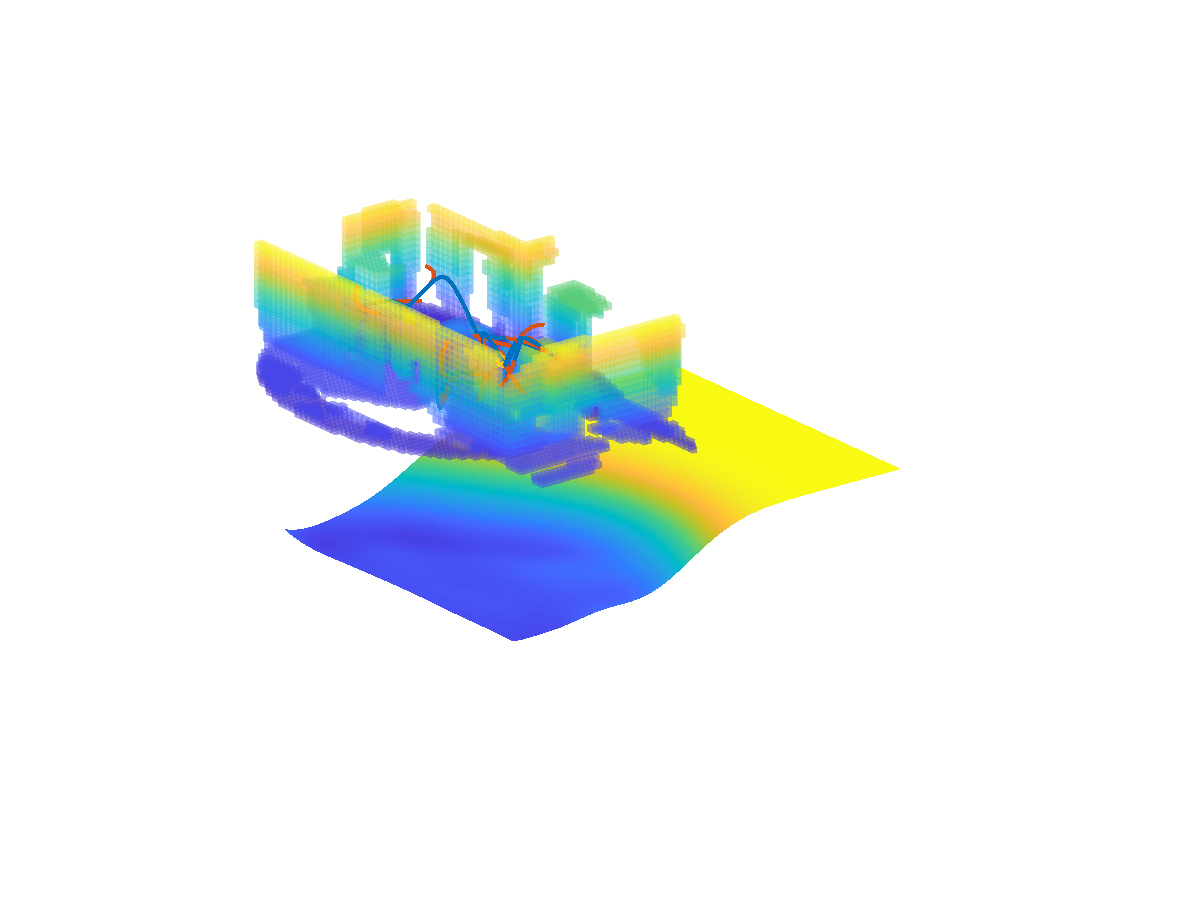
\includegraphics[trim={3cm 1.5cm 3cm 1cm}, clip = true, width = 1.2\textwidth]{Figs/Chapter4/exploration_100s.eps}}
		\end{minipage}
		\begin{minipage}{.4\linewidth}
			\centering
			\subfloat[]{%
				\label{FIG:EXPLORATION-SIM-TEST-B}%
				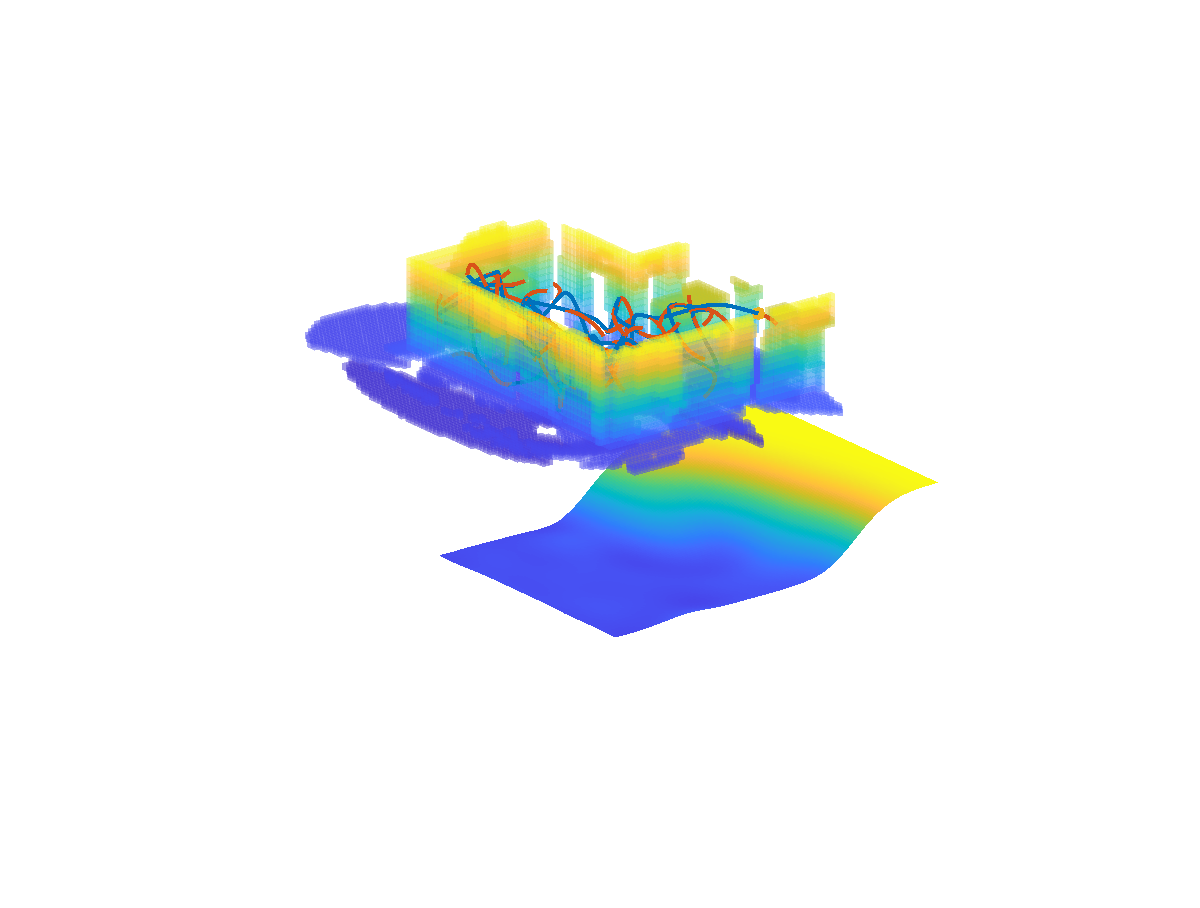
\includegraphics[trim={5cm 1.5cm 3cm 1cm}, clip = true, width = 1.2\textwidth]{Figs/Chapter4/exploration_200s.eps}}
		\end{minipage}
		\begin{minipage}{.4\linewidth}
			\centering
			\subfloat[]{%
				\label{FIG:EXPLORATION-SIM-TEST-C}%
				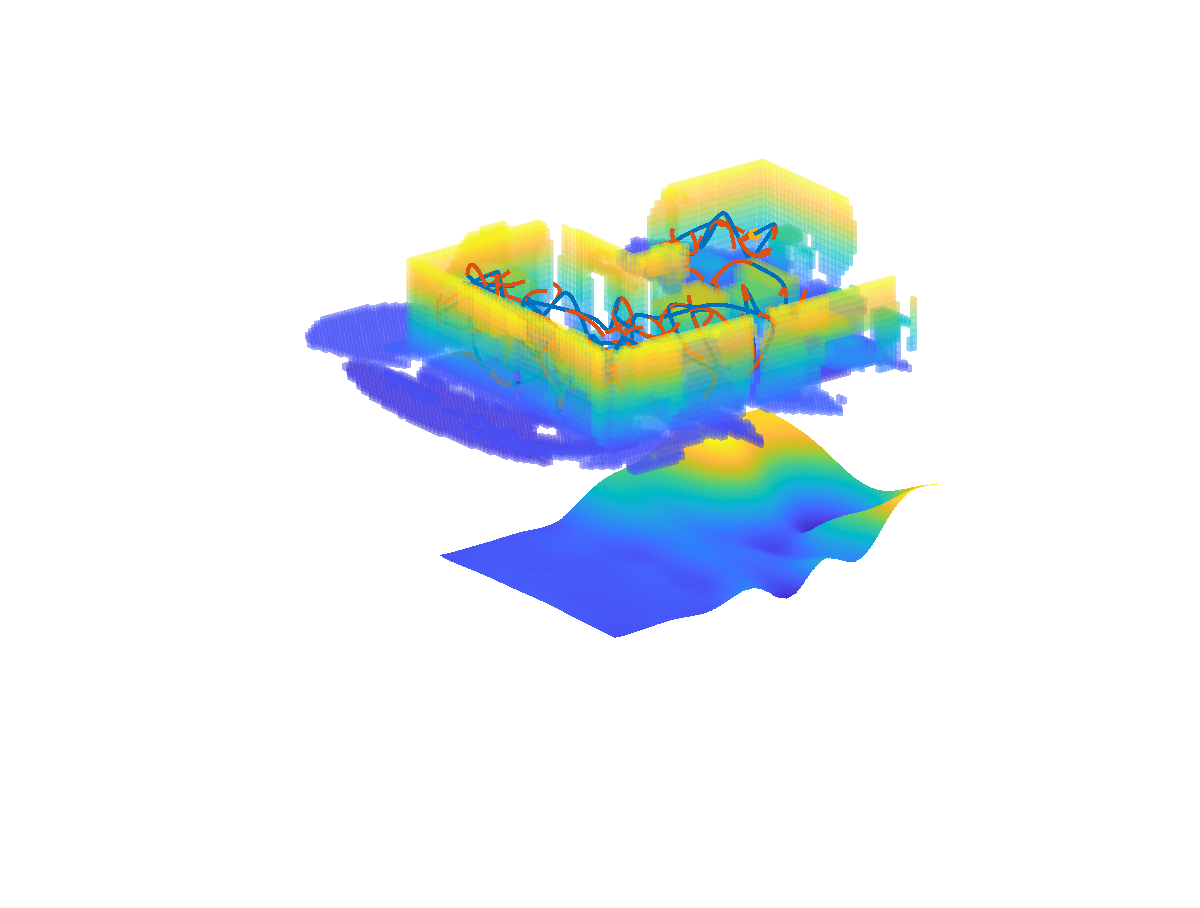
\includegraphics[trim={5cm 1.5cm 3cm 1cm}, clip = true, width = 1.2\textwidth]{Figs/Chapter4/exploration_300s.eps}}
		\end{minipage}
	\end{center}
	\caption{Results of the simulation tests. The exploration algorithm runs over a map of $20\times10\times3$
	meters and was able to complete the exploration after only $400$ seconds. In the image, in order,
	(a) exploration state at $100$ seconds, (b) exploration state at $200$ seconds, and (c) exploration state at $300$ seconds.
	At the bottom of each time snapshot, a visual representation of the Gaussian inferred information gain is reported.
	}\label{FIG:EXPLORATION-SIM-TEST}
\end{figure}
%%%%%%%%%%
%%%%%%%%%%
\begin{figure}[!t]
	\begin{center}
		\begin{minipage}{.4\linewidth}
			\centering
			\subfloat[]{%
				\label{FIG:EXPLORATION-REAL-TEST-A}%
				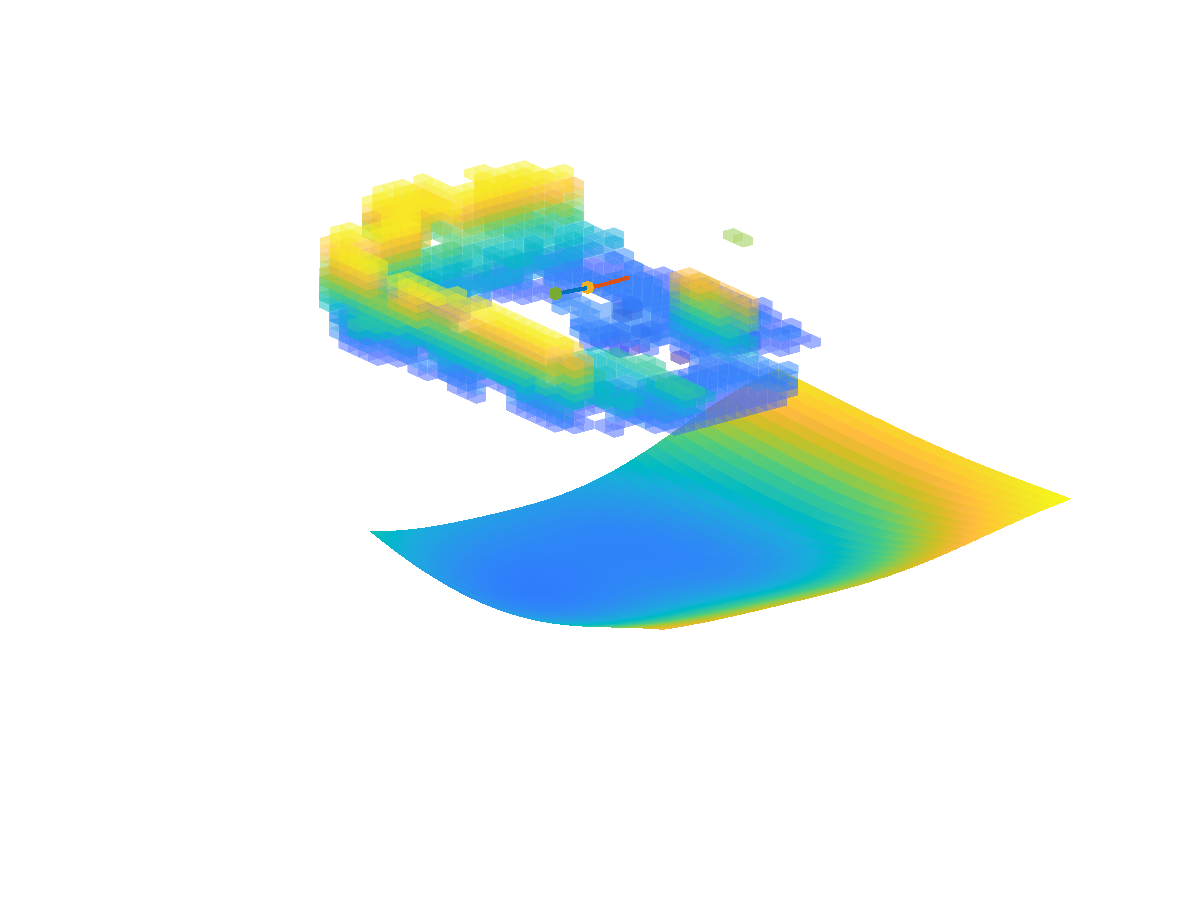
\includegraphics[trim={5cm 1.5cm 2cm 2.2cm}, clip = true, width = 1\textwidth]{Figs/Chapter4/20s.eps}}
		\end{minipage}
		\begin{minipage}{.4\linewidth}
			\centering
			\subfloat[]{%
				\label{FIG:EXPLORATION-REAL-TEST-B}%
				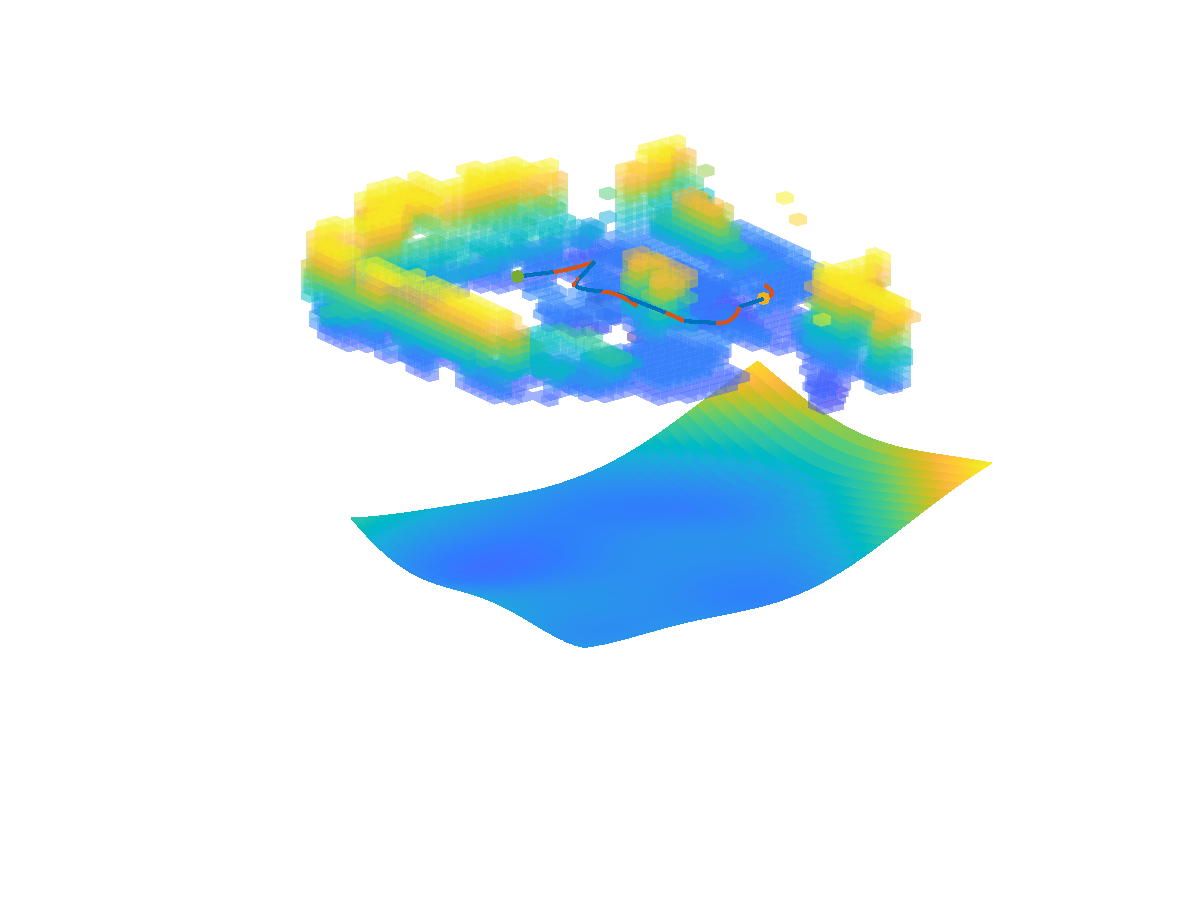
\includegraphics[trim={5cm 1.5cm 3cm 2.2cm}, clip = true, width = 1\textwidth]{Figs/Chapter4/57s.eps}}
		\end{minipage}
		\begin{minipage}{.4\linewidth}
			\centering
			\subfloat[]{%
				\label{FIG:EXPLORATION-REAL-TEST-C}%
				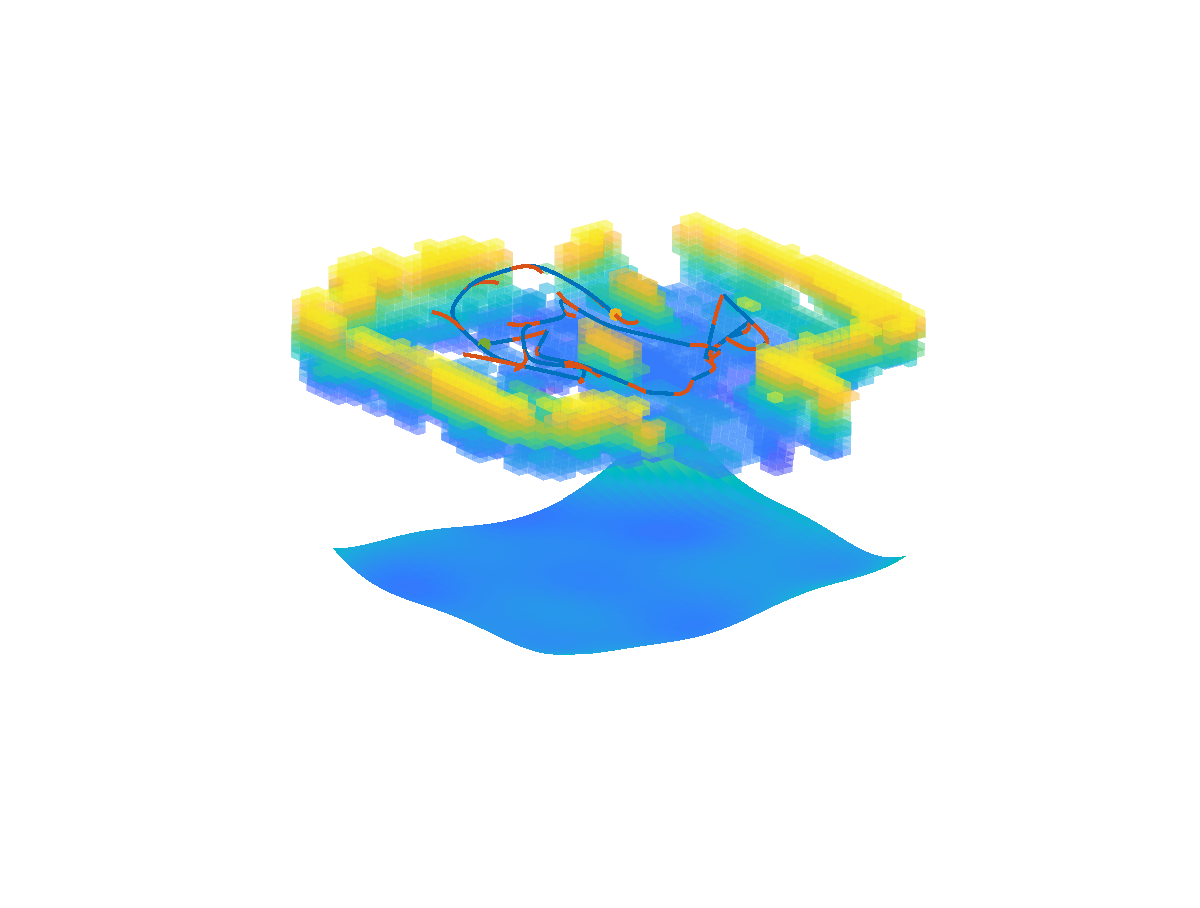
\includegraphics[trim={5cm 1.5cm 3cm 2.2cm}, clip = true, width = 1\textwidth]{Figs/Chapter4/167s.eps}}
		\end{minipage}
	\end{center}
	\caption{Results of the real-world exploration test. The exploration algorithm was run using only integrated onboard
	sensors and computational capabilities. In the image, in order, (a) exploration state at $20$ seconds,
	(b) exploration state at $57$ seconds, and (c) exploration state at $167$ seconds.
	At the bottom of each time snapshot, a visual representation of the Gaussian inferred information gain is reported.
	}\label{FIG:EXPLORATION-REAL-TEST}
\end{figure}
%%%%%%%%%%
The parameters used during the simulation tests are reported in~\tabref{TAB:EXPLORATION-SIMULATION-PARAMETERS}.~\figref{FIG:EXPLORATION-SIM-TEST}
shows the obtained simulation results when agent is required to map an $20\times10\times3$
urban canyon. In particular, in~\figref{FIG:EXPLORATION-SIM-TEST}, the blue lines represent the reference trajectory, the red
ones are the planned safe motions (both executed and non-executed), while the bottom surface represents the current Gaussian
process state. It can be noticed that, the Gaussian process is constantly kept updated with the current map information and it
results to be consistent, at each time instant, with the exploration task. In order to evaluate the performances against the
state-of-the-art solutions, the proposed algorithm has been compared with the \emph{Autonomous Exploration Planner} (AEP)
described in~\cite{selin2019efficient}.~\figref{FIG:EXPLORATION-COMPARED-ALGOROTHMS} compares the amount of explored volume
over time by both the approaches. The blue line represents the average of explored area obtained deploying our approach over $10$
experiments, with the associated standard deviation represented in shaded blue. Conversely, the line and shade red reports the
results obtained via AEP, with the global exploration module disabled, on the same number of experiments. It can be noticed that
both algorithms achieve comparable results at the beginning of the exploration, where most of the volume needs to be explored,
then our solution tends to get higher exploration rate, thanks to the ability to fast plan the next trajectory. Moreover, it is
worth noting that our solution provides more consistency between different tests, as the variance is narrower with respect to the AEP,
thus guaranteeing better repeatability of the experiment and a mitigation of the worst case scenarios.
\figref{FIG:EXPLORATION-TRAVELLED-DISTANCE} depicts the overall travelled distance on same experiments. Since our solution plans
trajectories by never stopping the UAV motion, this leads to an overall travelled distance $2$ times higher than the AEP solution.
%%%%%%%%%%%
\begin{figure}[!t]
	\centering
	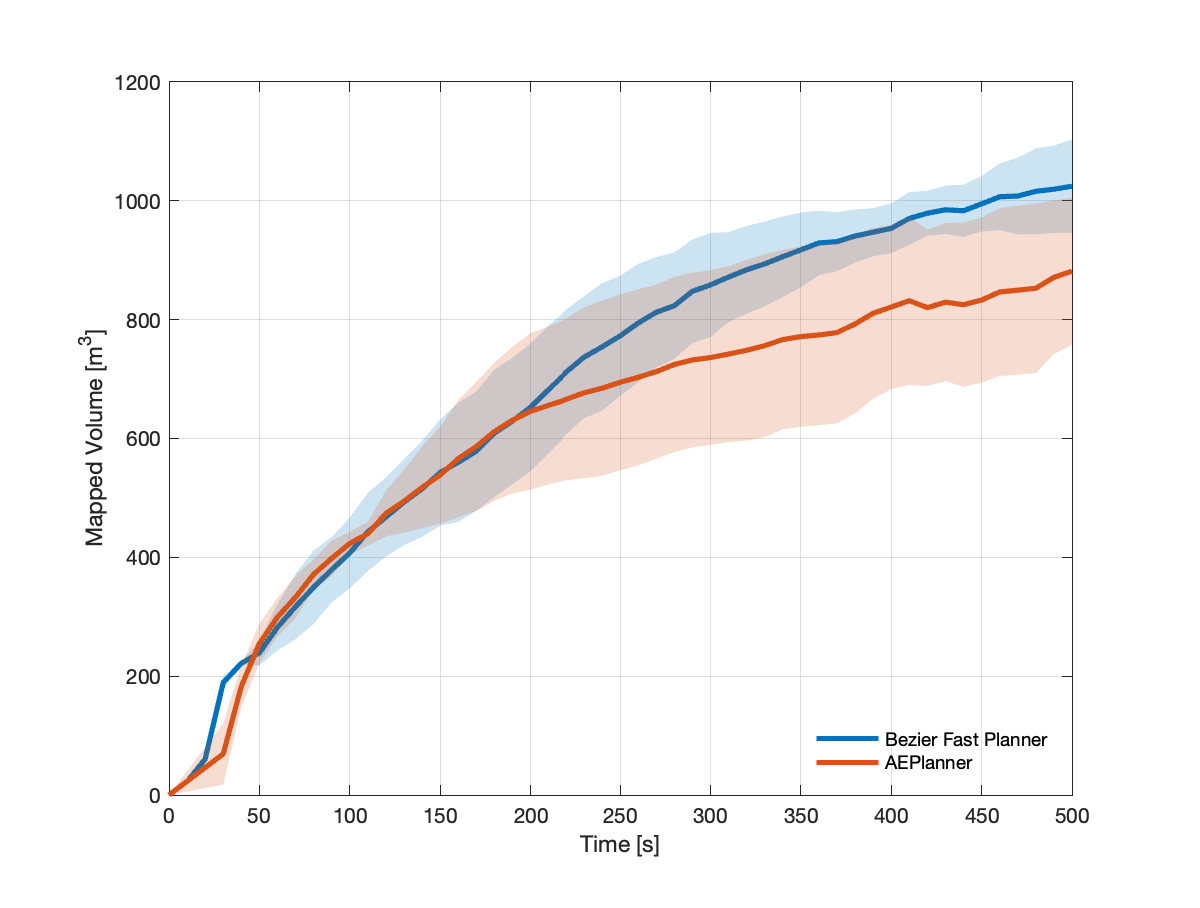
\includegraphics[trim={0cm 0cm 0cm 1cm}, clip = true, scale=.4]{Figs/Chapter4/mapped_volume.eps}
	\caption{Exploration progress for the urban $20 \times 10 \times 3$ canyon. Mean and standard deviation over $10$
	experiments are shown. Notice that due to the employing of pierced nets as maps borders makes the overall explored
	volume higher than the real volume.}%
	\label{FIG:EXPLORATION-COMPARED-ALGOROTHMS}
\end{figure}
\begin{figure}[!t]
	\centering
	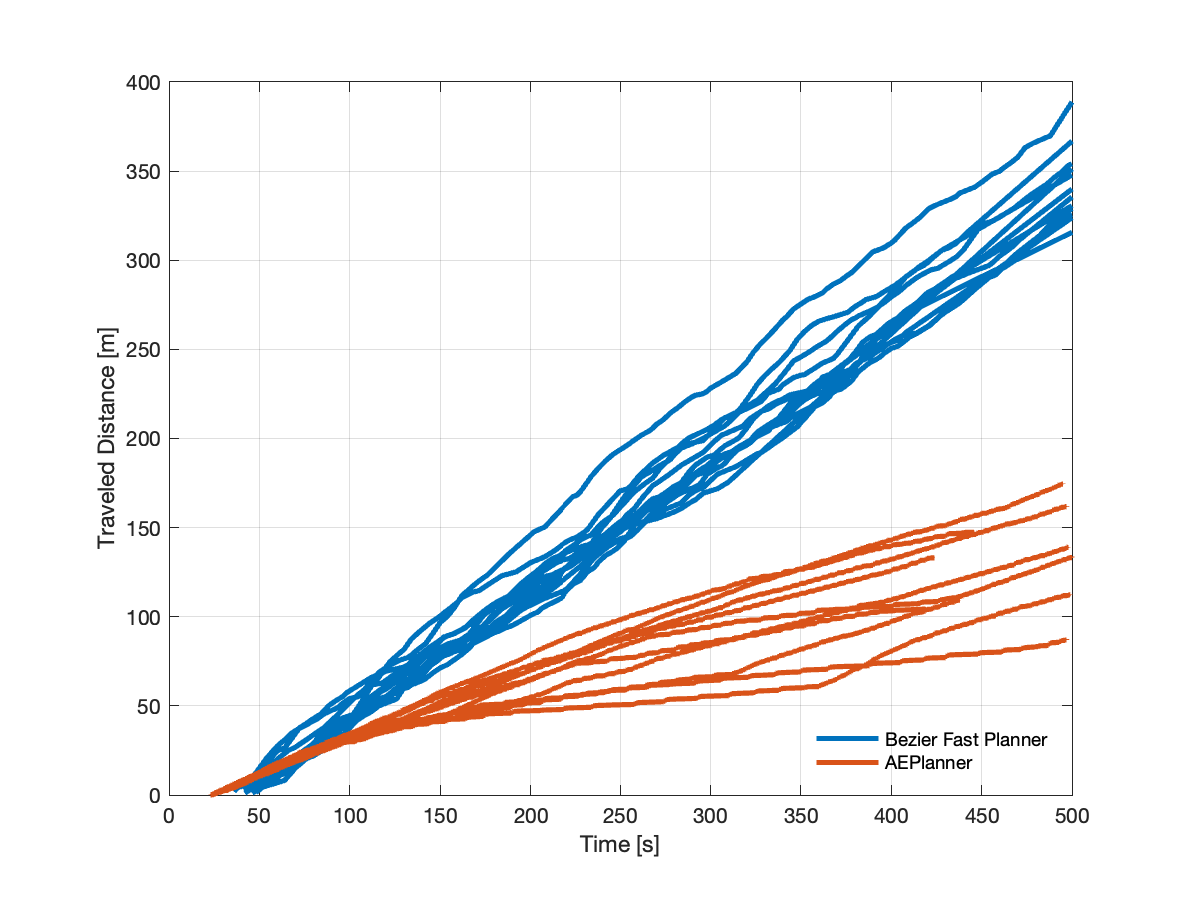
\includegraphics[scale=.4]{Figs/Chapter4/traveled_distance.eps}
	\caption{Overall traveled distance in the urban canyon. The traveled distances over $10$ experiments are shown.}%
	\label{FIG:EXPLORATION-TRAVELLED-DISTANCE}
\end{figure}
%%%%%%%%%%%
The solution has been tested using a real UAV inside an indoor scenario using our office spaces.
The obtained results are depicted in~\figref{FIG:EXPLORATION-REAL-TEST}. The used parameters are reported
in~\tabref{TAB:EXPLORATION-REAL-PARAMETERS}. The available area was $9\times6\times2.5$ meters and it was successfully
mapped in $170$ seconds, the maximum camera range was saturated at $3$ meters in order to stress navigation trajectories around
obstacles. The used UAV was powered by the PX4 autopilot and endowed with a depth Intel RealSense D455 camera, mounted frontally.
Visual odometry, used to localize the UAV in the indoor scenario, was provided by an Intel Realsense T265 tracking camera. 

%----------------------------------------------------------------------------------------
\section{Patrolling: A Different Exploration Perspective}%
\label{SEC:SEARCH-PATROLLING-PERSPECTIVE}
In this section, we review a novel and different solution to the exploration problem stated in~\secref{SEC:EXPLORATION-PROBLEM-DEFINITION},
in the setting where the environment is completely known and the only goal is to find out interesting points, or objects,
inside the explored area. In this framework, the general exploration problem can be specialised by considering a third attribute, jointly
with \emph{free} and \emph{occupied}, namely \emph{interest}. A subset of the overall volume $\V \in \R^3$ will be categorised as
$\V_{\text{int}} = \{ \xx \in \V \mid \Gamma(\xx) = \text{int} \}$, thus the exploration task will be considered complete when
$\V_{\text{free}} \cup \V_{\text{occ}} \cup \V_{\text{int}} = \V \setminus \V_{\text{res}}$, with $\V_{\text{free}}$, $\V_{\text{occ}}$,
and $\V_{\text{res}}$ defined as in~\secref{SEC:EXPLORATION-PROBLEM-DEFINITION}.
Let us suppose to completely apriori known the set $\V_{\text{free}}$, then the exploration goal reduces to correctly classify
$\V \setminus \V_{\text{res}} \setminus \V_{\text{free}}$ between $\V_{\text{occ}}$ and $\V_{\text{int}}$.
The proposed approach is based on the idea that the employed software pipeline used to recognise the objects of interest may fail
in doing that, and the probability of failure is jointly linked with the capability of the endowed sensor. Moreover, the autonomous
platform may not be able to perform the commissioned motion due to environment modifications, or unexpected and unmapped obstacles.
The stochastic nature of the problem at hand, along with the stochasticity of the adopted pipeline, embraces a purely probabilistic
approach, so the locations of the objects are expressed in a likelihood form, that in the following takes the name of
\emph{probabilistic map}.

Similar to the algorithm described in~\secref{SEC:EXPLORATION-LARGE-SCALE}, the core of the proposed solution consists of an RRT of
possible and feasible motions. Unlike the previous approach, here we do not constrain the tree to directly represents pieces of
possible trajectories. In this case, the tree is built to describe possible collision-free paths inside the environment, while the
computation of the associated timing laws is left as next step, during the \emph{trajectory optimisation} stage. In this view,
the timing law is selected to ensure trajectory feasibility in terms of induced maximum velocity and acceleration.
The tree expansion is supplied with the aforementioned probabilistic map, which is copied and kept updated on each new sampled
node. The extension of the node attributes set with a copy of the current likelihood map allows for time consistency.
The map in each node is in fact constantly kept updated, allowing for cost increase or decrease if the exploration time grows, or 
if a particular node has been visited, respectively.
The remainder of this section unfolds as follows~\secref{SEC:SEARCH-MAP-STRATEGY} and~\secref{SEC:SEARCH-COMPLEXITY-REDUCTION}
deeply analyze the aforementioned mapping strategy, bridging the gap between discrete and continuous maps, and proposing a novel
mapping framework. In~\secref{SEC:SEARCH-TREE-STRUCTURE} the tree structure is briefly described, along with the adopted growth
policy,~\secref{SEC:SEARCH-TRAJECTORY-OPTIMISATION} introduces the used time allocation procedure and how the final trajectory is iteratively
refined before its commissioning. Finally,~\secref{SEC:SEARCH-EXPERIMENTAL-RESULTS} reports the obtained results when the proposed
approach is exploited to perform target search in a completely known environment.

\subsection{Mapping Strategy}%
\label{SEC:SEARCH-MAP-STRATEGY}
%%%%%%%%%%%
\begin{figure}[!t]
	\centering
	\includegraphics[width=0.8\textwidth]{Figs/Chapter4/camera_fov.pdf}
	\caption{Probabilistic adopted camera model.}
	\label{FIG:SEARCH-CAMERA-MODEL}
\end{figure}
%%%%%%%%%%%
In this solution we employ a discrete occupancy-based mapping approach~\cite{hornung2013octomap} to store information about occupied
and free spaces, while interesting environment features, or objects, are stored by following a continuous probability mapping paradigm.
In particular, Gaussian processes are used to infer the belief of features existence. This approach allows to increase the map
reliability by introducing spatial correlations between data while maintaining the memory consumption low, and to formulate an information
gain that trades-off between target re-observation and exploration for new ones.
In a probabilistic framework, the target positions are usually represented through a set of discrete random variables defined over a
discretization of the search space ($\E \subset \R^3$). This approach leads to a discrete occupancy map ($\M$) where each grid cell is associated with
an independent Bernoulli random variable ($\bernoulli_i$) whose Probability Mass Function (PMF) represents the probability of target
occupancy~\cite{popovic2020informative}
\begin{equation*}
	\Prob \lp \bernoulli_i = k \rp =
	\begin{cases}
		\prob_i &\text{if } k=1, \\
		1 - \prob_i &\text{if } k=0.
	\end{cases}
\end{equation*}
The value of $\prob_i$ for each $\bernoulli_i \in \M$ inside the sensor FoV is updated, at each new sensor measurement,
via the Bayes formula
\begin{equation*}
	\Prob \lp \bernoulli_i \mid z^{1:t}, s^{1:t} \rp = \frac{\Prob \lp z^{t} \mid \bernoulli_i, s^t \rp
													   \Prob \lp \bernoulli_i \mid z^{1:t-1}, s^{1:t-1} \rp}{\Prob \lp z^t \rp},
\end{equation*}
where $z^t$ is the current observation at sensor position $s^t$. The aforementioned relation is usually rewritten in
log-likelihood notation, where products are replaced by additions, allowing for faster updates~\cite{hornung2013octomap}
\begin{equation}
	\label{EQ:SEARCH-LOG-LIKELIHOOD}
	\like \lp \bernoulli_i \mid z^{1:t}, s^{1:t} \rp = \like \lp \bernoulli_i \mid z^{1:t-1}, s^{1:t-1} \rp +
													   \like \lp z^t \mid \bernoulli_i, s^t \rp,
\end{equation}
with
\begin{equation*}
	\like \lp \bernoulli_i \rp = \log \lp \frac{\Prob \lp \bernoulli_i = 1 \rp}{1-\Prob \lp \bernoulli_i = 1 \rp} \rp.
\end{equation*}
In~\eqqref{EQ:SEARCH-LOG-LIKELIHOOD} the quantities $\like \lp \bernoulli_i \mid z^{1:t-1}\rp$ and
$\like \lp \bernoulli_i \mid z^{1:t}\rp$ represent the prior and posterior probability, respectively.
While, $\like \lp z^t \mid \bernoulli_i \rp$ is the observation likelihood that strongly depends on the adopted probabilistic
sensor model. In our specific case, we employ a downward-facing monocular camera to detect targets on the ground,~\figref{FIG:SEARCH-CAMERA-MODEL}
shows the probabilistic model for such type of sensor. The probability to retrieve correct measures decreases approaching the FoV boundaries,
as well as the maximum distance allowed. This kind of behavior is well described by a modified logistic function of the kind
\begin{equation*}
	\Prob \lp z^t = 1 \mid \bernoulli_i, s^t \rp = 0.5 + \frac{\prob_{\text{max}}}{1 + \exp \lp \norm{x_i - s^t}_{W} - c \rp},
\end{equation*} 
where $x_i \in \M$ represents the grid cell associated with $\bernoulli_i$, while $s^t \in \R^3$ is the current sensor position.
The weight matrix $W \in \R^{3 \times 3}$, and the parameters $\prob_{\text{max}}$ and $c$ are responsible to shape the function
over the camera field of view.

Despite the power of discrete maps, in our solution we choose to adopt a continuous mapping strategy.
Continuous maps allow to incorporate spatial correlations of input data and, potentially, require lower memory to maintain the overall map.
These advantages are not for free since continuous maps present a higher computational complexity. Gaussian processes are well suited for
this purpose since can encode spatial correlations in a probabilistic way and, with a careful choice of training points, take low
computational and storage memory. With this idea in mind, the log-likelihood of occupancy is treated, in this case, as a continuous
function over the search space $\like:\E \subset \R^3 \mapsto \R$. The key idea is to model such function as a realization of a Gaussian
process. A GP model is completely defined by a mean function $\prior \lp \xx \rp: \E \mapsto \R$ and a covariance function
$\kf \lp \xx, \xx' \rp: \E \times \E \mapsto \R$
\begin{align*}
	\like \lp \xx \rp \sim \GP \lp \prior \lp \xx \rp, \kf \lp \xx,\xx' \rp \rp.
\end{align*}
Although there are many possible choices for mean and covariance functions, usually the structure of $\prior$ and $\kf$ are assumed to be
known up to certain hyper-parameters ($\prior \lp \cdot, \param_{\prior} \rp$, $\kf \lp \cdot, \param_{\kf} \rp$).
In the particular case of target search, the mean function should be chosen on the basis of some a prior notions about the target existence,
thus it is a priori fixed and does not depend on any hyper-parameter. In those cases in which no prior information is available,
the mean function is simply $\prior \lp \xx \rp = 0$  $\forall \xx \in \E$, that corresponds to an occupancy probability of $0.5$.
The covariance function, aka \textit{kernel}, influences the GP behavior when fed with training data points.
The results presented afterward are obtained using a \textit{Matérn $3/2$ kernel}, that takes the form
\begin{equation*}
	\kf  \lp \xx, \xx', \param \rp = \lp 1 + \frac{\sqrt{3} d}{\param} \rp \exp \lp - \frac{\sqrt{3} d }{\param} \rp, 
\end{equation*}
where $d = \norm{\xx - \xx'}^2_2$, while $\param$ is a hyper-parameter known as \textit{characteristic length-scale}~\cite{rasmussen2003gaussian}.
The Matérn $3/2$ kernel is very common in geostatistical analysis, due to its capability to capture discrete targets~\cite{meera2019obstacle},
thus it results very suitable also for this particular application. Given $\nsample$ noisy observations $\yy^{1:\nsample} \in \R^{\nsample}$
and the respective sampling locations $\xx^{1:\nsample} \in \R^{\nsample \times 3}$, the posterior distribution of $\like$ is a Gaussian distribution,
whose mean and variance can be evaluated as
\begin{align}%
	\label{EQ:SEARCH-POST-MEAN}
	\pmu \lp \xx \rp & = \prior \lp \xx \rp + \kv \lp \xx \rp\T \lps \km + \nn I \rps^{-1}
						 \lp \yy^{1:\nsample} - \prior \lp \xx^{1:\nsample} \rp \rp, \\
	\label{EQ:SEARCH-POST-VARIANCE}
	\pvar \lp \xx \rp & = \kf \lp \xx,\xx \rp - \kv \lp \xx \rp\T \lps \km + \nn I \rps^{-1} \kv \lp \xx \rp.
\end{align}
To deal with the unknown hyper-parameter, we follow an empirical Bayes approach~\cite{benevento2020multi}, where the prediction steps are
alternated with parameters estimation steps via maximum likelihood
\begin{equation*}
	\param = \arg\max_{\param}  \prob \lp \yy^{1:\nsample} \mid \xx^{1:\nsample}; \param \rp.
\end{equation*}
Under the Gaussian process prior, the quantity $\prob \lp \yy^{1:\nsample} \mid \xx^{1:\nsample}; \param \rp$ can be evaluated in closed
form as log-likelihood (dropping the apex $^{1:\nsample}$)
\begin{equation*}
	\begin{split}
		& \log \lp \prob \lp \yy \mid \xx; \param \rp \rp = \\
		& \hspace{1cm} -\frac{1}{2} \lp \prior \lp \xx \rp - \yy \rp \T \lps \km + \nn I \rps^{-1} \lp \prior \lp \xx \rp - \yy \rp\\
		& \hspace{1cm} -\frac{1}{2} \log \lp \lb \km + \nn I \rb \rp - \frac{\nsample}{2}\log \lp 2\pi \rp.
	\end{split}
\end{equation*}

\subsection{Complexity Reduction \& Spatial Partitioning}%
\label{SEC:SEARCH-COMPLEXITY-REDUCTION}
%%%%%%%%%%
\begin{figure}[!t]
	\centering
	\includegraphics[width=0.6\textwidth]{Figs/Chapter4/map_discretization.pdf}
	\caption{2-Dimensional example of the adopted environment discretization.
			 In this particular case, the presence of a target makes the likelihood level increases in that area, leading to a
			 finer adopted discretization.}
	\label{FIG:SEARCH-SPACE-DISCRETIZATION}
\end{figure}
%%%%%%%%%%
Exact GP inference is expensive due to matrix inversion, whose computational complexity scales with the number of training points as
$\mathcal{O} \lp \nsample^3 \rp$. Moreover, after training, the computation of posterior mean~\eqref{EQ:SEARCH-POST-MEAN} and
variance~\eqref{EQ:SEARCH-POST-VARIANCE} costs $\mathcal{O}\lp \nsample \rp$ and $\mathcal{O} \lp \nsample^2 \rp$ respectively,
per testing point. This makes the application of GP regression in real-time challenging, in particular for large environments.
The common approach to deal with this issue was to divide the environment into regions and train several experts, one for each
region~\cite{kim2013continuous}. This approach was effective, but the complexity problem still persists as long as the number of
observations per region increases. Recently, approaches that leverage on \textit{approximate regression} have shown great success
thanks to their good scaling capabilities~\cite{quinonero2005unifying, wilson2015kernel, gardner2018product}.
To reduce the GP complexity, the adopted approach leverages on the Subset of Regressors (SoR) method~\cite{quinonero2005unifying}
to compute an approximation of the gram matrix $\km$ and the kernel vector $\kv$, jointly with a spatial partitioning and a targeted choice
of the training points. In particular, a set of $\ninducing$ \textit{inducing variables} ($\uu^{1:\ninducing} \in \R^{\ninducing\times3}$)
are arbitrarily selected out of the training points set ($\xx^{1:\nsample}$), then the covariance quantities can be approximated as
\begin{equation}%
	\label{EQ:SEARCH-SOR-APPROX}
	\begin{split}
		\km & \sim \km_{\xx\uu}  \km_{\uu\uu}^{-1} \km_{\uu\xx},\\
		\kv \lp \xx \rp & \sim \km_{\xx\uu} \km_{\uu\uu}^{-1} \kv_{\uu} \lp \xx \rp.
	\end{split}
\end{equation}
Where $\km_{\uu} \in \R^{\ninducing \times \ninducing}$ and $\kv_{\uu} \in \R^{\ninducing}$ are the covariance matrix and vector computed
along the inducing points, while $\km_{\xx\uu} \in \R^{\nsample \times \ninducing}$ is the cross-covariance between $\xx^{1:\nsample}$ and
$\uu^{1:\ninducing}$, with entries
\begin{equation*}
	\km^{i,j}_{\xx\uu} = \kf \lp \xx^i, \uu^j \rp \text{ with } i \in \lps 1, \nsample \rps \text{ and } j \in \lps 1, \ninducing \rps.
\end{equation*}
Plugging~\eqqref{EQ:SEARCH-SOR-APPROX} in~\eqqref{EQ:SEARCH-POST-MEAN} and~\eqqref{EQ:SEARCH-POST-VARIANCE} leads to
\begin{align*}
		\pmu \lp \xx \rp & = \prior \lp \xx \rp + \kv_{\uu} \lp \xx \rp\T \lps \km_{\uu\xx}\km_{\xx\uu} + \nn \km_{\uu\uu} \rps^{-1} \km_{\uu\xx} \cdot \\
						& \hspace{5cm} \cdot \lp \yy^{1:\nsample} - \prior \lp \xx^{1:\nsample} \rp \rp, \\
		\pvar \lp \xx \rp & = \kv_{\uu} \lp \xx \rp\T \lps \km_{\uu\xx}\km_{\xx\uu} + \nn \km_{\uu\uu} \rps^{-1} \kv_{\uu} \lp \xx \rp.
\end{align*}
The SoR approximation method allows to reduce the computation complexity of the training procedure up to $\mathcal{O} \lp \nsample \ninducing^2 \rp$,
while the evaluation complexity of predictive mean and variance is kept constant ($\mathcal{O} \lp \nsample \rp$ and $\mathcal{O} \lp \nsample^2 \rp$,
respectively). The hyper-parameter estimation is carried out by maximizing the log-likelihood function evaluated just on the inducing points
($\log \lp \prob \lp \yy^{1:\ninducing} \mid \uu^{1:\ninducing}; \param \rp \rp$).
In order to further decrease the map computation complexity, we propose a novel methodology to proper select the expert training points.
A good approach should trade-off between process complexity and map precision. To achieve that, the 3-dimensional environment is discretized
with a very coarse resolution, then we let this discretization be flexible in areas where higher precision is required.
The discretization level is then dependent on the local likelihood value: higher is the probability of target existence and finer is the adopted
discretization. In particular, the probability range $[0,1]$ is divided into $q$ intervals, each of which corresponds to a given map resolution.
Note that those intervals are such that a discretization level and the consecutive one differ of a factor equal to $2$.
This leads to a quad-tree space discretization (see~\figref{FIG:SEARCH-SPACE-DISCRETIZATION}). Training points are store in memory only when a
measure of them is retrieved, each new point inherits the current local GP value, then is updated at each new sensor measurement
through~\eqqref{EQ:SEARCH-LOG-LIKELIHOOD}. The adopted hierarchical structure allows to select the inducing variables as those training
points obtained from the coarsest discretization, associated with null probability. Moreover, when a training point gets a promotion to the
upper discretization level, that point is also promoted to inducing variable, while a set of new training points are added to still be
compliant with the associated discretization level.

\subsection{Tree Structure \& Update}%
\label{SEC:SEARCH-TREE-STRUCTURE}
The proposed algorithm works by iteratively growing an RRT, $\tree = \lp \nodes, \edges \rp$, of possible feasible motions,
whose each node $\node_i \in \nodes$ is described by means of six quantities
\begin{equation*}
	\node_i = \left\{ g_i, c_i, \rr_i, \yy_i^{1:\nsample}, \xx_i^{1:\nsample}, \uu_i^{1:\ninducing} \right\},
\end{equation*}
where $g_i = g\lp \node_{i-1}, \node_i \rp$ and $c_i = c\lp \node_{i-1}, \node_i \rp$ are the information gain and the cost,
respectively, associated with the execution of node $\node_i$, i.e. navigate from $\node_{i-1}$ to $\node_i$.
The quantity $\rr_i \in \R^3$ describes the node position, while $\yy_i^{1:\nsample}$, $\xx_i^{1:\nsample}$,
and $\uu_i^{1:\ninducing}$ represent the parameterisation of the likelihood map, at the time of node creation.
As already mentioned, unlike the approach described in~\secref{SEC:EXPLORATION-LARGE-SCALE}, here the adopted tree does not directly
represent a set of possible trajectories, but instead describes a set of feasible paths through the environment.
As a matter of fact, the aforementioned node description does not take into account neither a trajectory parameterisation, nor a
possible execution time. In this sense, two nodes $\node_{i-1}$ and $\node_i$ are connected by an edge $\edge_{i-1}$ if the straight path
connecting $\rr_{i-1}$ and $\rr_i$ is collision-free, no other continuity constraints are required.
Although the nodes present a slight different structure, the aim of this tree is the same of the one build in~\secref{SEC:EXPLORATION-TREE-STRUCTURE}.
Basically, the goal is to compute sub-optimal paths that maximise a given utility function $\loss \lp \RR \lp \node_i \rp \rp$, with
the latter that combines gains and costs of all nodes in $\RR \lp \node_i \rp$. It results that the final agent behavior strongly depends
on the chosen functions $g \lp \node_{i-1}, \node_i \rp$, $c \lp \node_{i-1}, \node_i \rp$ and $\loss \lp \RR \lp \node_i \rp \rp$.
Unlike general planners, who exploit RRT structures to plan flyable trajectories, in this case the tree expansion logic
must be designed around the aforementioned loss functions, with particular attention to the gain $g \lp \node_{i-1}, \node_i \rp$.
Tailoring the algorithm behavior on $g$ allows for keeping the exploration task consistent during the motion, and avoids cases
in which the agent gets stuck in little areas, without exploring the overall environment. This is particularly true when the
chosen utility function presents many local minima, which are difficult to escape.
In this respect, we formulate a new information gain index that takes into account the amount of improvement, in the current
likelihood map, brought by the execution of the considered node. In particular, consider two nodes $N_{i-1}$ and $N_i$,
with their respective map parameterisation $\pmu_{i-1} \lp \yy_{i-1}^{1:\nsample}, \xx_{i-1}^{1:\nsample}, \uu_{i-1}^{1:\ninducing}, \xx \rp$
and $\pmu_{i} \lp \yy_{i}^{1:\nsample}, \xx_{i}^{1:\nsample}, \uu_{i}^{1:\ninducing}, \xx \rp$, the gain associated with the
node $\node_i$ can be evaluated as
\begin{equation*}
	g_i \lp \node_i, \node_{i-1} \rp = \int_{\E} \frac{\exp \lp \pmu_{i-i} \lp \cdot, \xx \rp \rp}{1 + \exp \lp \pmu_{i-i} \lp \cdot, \xx \rp \rp} -
								  	   \frac{\exp \lp \pmu_i \lp \cdot, \xx \rp \rp}{1 + \exp \lp \pmu_i \lp \cdot, \xx \rp \rp} d\xx,
\end{equation*}
where the quantities $\yy_{i}^{1:\nsample}$, $\xx_{i}^{1:\nsample}$, and $\uu_{i}^{1:\ninducing}$ are computed out of the corresponding
values of the $\node_{i-1}$ node via~\eqqref{EQ:SEARCH-LOG-LIKELIHOOD}, along the path connecting $\rr_{i-1}$ to $\rr_i$.
Note that, unlike previous works in this field~\cite{popovic2020informative, schmid2020efficient}, here the information gain is not
a function of the node end-position only, thus allows us to consider also frustrum overlap between consecutive poses and the amount of
information gained while moving from $\node_{i-1}$ to $\node_i$.
On the other hand, the node execution cost is fixed as the intra-node Euclidean distance $c_i \lp \node_i, \node_{i-1} \rp = \norm{\rr_{i-1} - \rr_i}$,
while the total utility function as been designed following the same idea of efficiency stated in~\secref{SEC:EXPLORATION-COST-FUNCTIONS}
\begin{equation*}
	\loss \lp \RR(\node_i) \rp = \frac{\sum_{\node_l \in \RR \lp \node_i \rp} g_l}{\sum_{\node_l \in \RR \lp \node_i \rp} c_l}.
\end{equation*}
With these notion at hand, we can now proceed to the design of the core of the algorithm. The chosen tree updating procedure is
as simple as it is effective, and it is designed to cope with the multi-modal nature of the chosen utility function, as well as
the possibility to inject prior notions about the obstacles occupancy. The tree, initially composed of just one root node, is
iteratively expanded via random sampling of the next node position $\rr_i$. In particular, we constrain the sample points to lie
inside a circular crown of radii $R_{\text{min}}$ and $R_{\text{max}}$, centered on the current best node ($\node_{\text{best}}$),
namely the one among all tree nodes that maximise the utility function $\loss \lp \cdot \rp$. In order to escape from local minima
and let the tree grow in all directions, the best node is reevaluated each $n_{\text{sample}}$ samples, ensuring that every expanded
node presents exactly $n_{\text{sample}}$ childs. This choice, jointly with the circular crown constraint, allows the algorithm to
expand the tree without getting stuck in little areas, with many local minima.
Each sampled viewpoint is retained only if it belongs to a known and free part of the environment and, at the same time, the line
connecting it with the respective father is far enough from the mapped obstacles. The tree expansion continues until
the number of sampled nodes goes beyond a given threshold $n_{\text{max}}$, then the path connecting the root node to the best one
is extracted and completely executed. It may happen that, the autonomous robot is not able to complete the commissioned path due 
to unexpected obstructions, in this case the algorithm keeps track of the executed nodes and reinitialize the tree with the 
final executed node as root.

\subsection{B-Spline Trajectory Optimisation}%
\label{SEC:SEARCH-TRAJECTORY-OPTIMISATION}
As already pointed out in previous sections, the built tree does not directly represent flyable trajectories, but just feasible paths
through the environment's obstacles. For the purpose of control, a timing law is essential to ensure the dynamic feasibility of the resulting
reference. In the specific case of a quadcopter, such a reference can be computed just in terms of heading angle $\yaw$ and space position
$\rr = \lps x, y, z \rps \in \R^3$, following the concept of differential flatness~\cite{mellinger2011minimum}. The latter property can
be used only if the heading trajectory is guarante to be at least a class $\CC^1$ function, while $\rr$ must be at least class $\CC^3$.
Contrary to the solution presented in~\secref{SEC:EXPLORATION-LARGE-SCALE}, here we enforce the use of B-splines as time parameterisation
tool for the planned collision-free path. B-splines are a generalization of B\acuteacc ezier curves which allows for a more compact
representation, especially when dealing with long trajectory segments. Unlike B\acuteacc ezier curves, B-splines are defined by a
set of control points $\CP = \lps \bs{\cpoint}_0, \dots, \bs{\cpoint}_{\cpnumber} \rps$, and a set of time knots
$\bs{\splinevar} = \lps \splinevar_0, \dots, \splinevar_{\cpnumber + \order + 1} \rps$, as
\begin{equation*}
	\bs{\spline} \lp \splinevar \rp = \sum_{i=0}^\cpnumber \basis_i^\order \lp \splinevar \rp \bs{\cpoint}_i,
\end{equation*}
with $\order$ order of the spline and $\basis_i^\order$ basis functions, recursively computed via the De-Boor formula~\cite{de1978practical}.
B-splines and B\acuteacc ezier curves share several properties, among all, the most important ones at the time being, are the
(a) convex hull containment and (b) closure with respect to differentiation. These two properties allow to easily formulate
a constrained quadratic programming problem and solve it for the final trajectory control points. A deeper analysis of B-spline properties and
their evaluation is reported in~\secref{SEC:SPLINES-APPENDIX}. In the specific case of patrolling, since we are using a downward-facing camera, the
heading trajectory loses importance, thus we consider it as a constant reference in time, and focus only on solving the optimisation problem
for the $x$, $y$, and $z$ components. Suppose to discretize the node sequence $\RR \lp \node_{\text{best}} \rp$ with a given resolution $\Delta_{\rr}$,
leading to a sequence of waypoints, $\rr_0, \cdots, \rr_{\cpnumber}$, moreover let $\order = 7$ and fix the knot vector as
\begin{equation*}
	\bs{\splinevar} =
	\begin{bmatrix}
		0_{0:7}, & \Delta_{\splinevar}, & 2\Delta_{\splinevar}, & \dots, & (\cpnumber-\order)\Delta_{\splinevar}, & T_{0:7}
	\end{bmatrix},
\end{equation*}
with $T = \sum_{i=0}^{\cpnumber-1} \norm{\rr_i - \rr_{i+1}}/v_{\text{max}}$ and $\Delta_{\splinevar} = T/(\cpnumber - \order + 1)$.
Then, the problem of feasible trajectory generation can be solved via the constrained quadratic programming
\begin{equation}%
	\label{EQ:SEARCH-OPTIMISATION-PROBLEM}
	\begin{split}
	\min_{\bs{\cpoint}_{0}, \dots, \bs{\cpoint}_{\cpnumber}} &
				\lambda_1 \int_0^{T} \norm{\frac{d^3 \bs{\spline} \lp \splinevar \rp}{d \splinevar^3}}^2 d \splinevar
				+ \lambda_2 \sum_{i=0}^{\cpnumber} \norm{\bs{\cpoint}_i - \rr_i}^2, \\
	\text{sub.to.} \hspace{0.3cm} &
				\bs{\cpoint}_i' \le v_{\text{max}} \hspace{0.3cm} \forall i = 0, \dots, \cpnumber-1, \\
				& \bs{\cpoint}_i'' \le a_{\text{max}} \hspace{0.3cm} \forall i = 0, \dots, \cpnumber-2, \\
				& \bs{\cpoint}_0 = \rr_0, \hspace{0.3cm} \bs{\cpoint}_{\cpnumber} = \rr_{\cpnumber}, \\
				& \bs{\cpoint}_0' = v_{\text{init}}, \hspace{0.3cm} \bs{\cpoint}_0'' = a_{\text{init}},
	\end{split}
\end{equation}
with $\lambda_{1,2} \in \R$ tuning parameters and $v_{\text{max}}$, $a_{\text{max}}$, $v_{\text{init}}$, and $a_{\text{init}}$ provided as
inputs. The aforementioned optimisation problem, framed in the context of quadcopter control, tries to compute minimal effort trajectories that
propagate in time close to the sampled waypoints. The B-spline properties are used here to constrain the dynamical quantities to strictly
remain inside the imposed structural limits and to shape the curve along the selected viewpoints.
Note that no final velocity nor acceleration constraints have been imposed, letting the algorithm select the optimal ones on its own.
This choice is motivated by the discussion carried out in~\secref{SEC:EXPLORATION-LARGE-SCALE}, where emerges that constraining the robot
to stop at each exploration step may degrade the algorithm performance.
As in the case of B\acuteacc ezier curves (see~\secref{SEC:EXPLORATION-COST-FUNCTIONS}), the loss function in
problem~\eqref{EQ:SEARCH-OPTIMISATION-PROBLEM} can be fully decomposed along the tree axis, yielding
\begin{equation*}
	\begin{split}
	\min_{\bs{\cpoint}_{0}, \dots, \bs{\cpoint}_{\cpnumber}} &
				\sum_{j}^{x,y,z} \lps \lambda_1 \int_0^{T} \lp \frac{d^3 \bs{\spline}_j \lp \splinevar \rp}{d \splinevar^3} \rp^2 d \splinevar
				+ \lambda_2 \sum_{i=0}^{\cpnumber} \lp \bs{\cpoint}_{j,i} - \rr_{j,i} \rp^2 \rps, \\
	\text{sub.to.} \hspace{0.3cm} &
				\text{Same of problem~\eqref{EQ:SEARCH-OPTIMISATION-PROBLEM}}.
	\end{split}
\end{equation*}
% For an eventually interested reader, a deeper analysis about this optimisation technique, how it can be implemented,
% extended and adapted to other use cases is reported in~\secref{SEC:TRAJECTORY-GENERATION}.

\subsection{Experimetal Results \& Future Directions}%
\label{SEC:SEARCH-EXPERIMENTAL-RESULTS}
%%%%%%%%%%
\begin{figure}[!t]
	\begin{center}
		\begin{minipage}{.4\linewidth}
			\centering
			\subfloat[]{%
				\label{FIG:SEARCH-RESULTS-MAP-A}%
				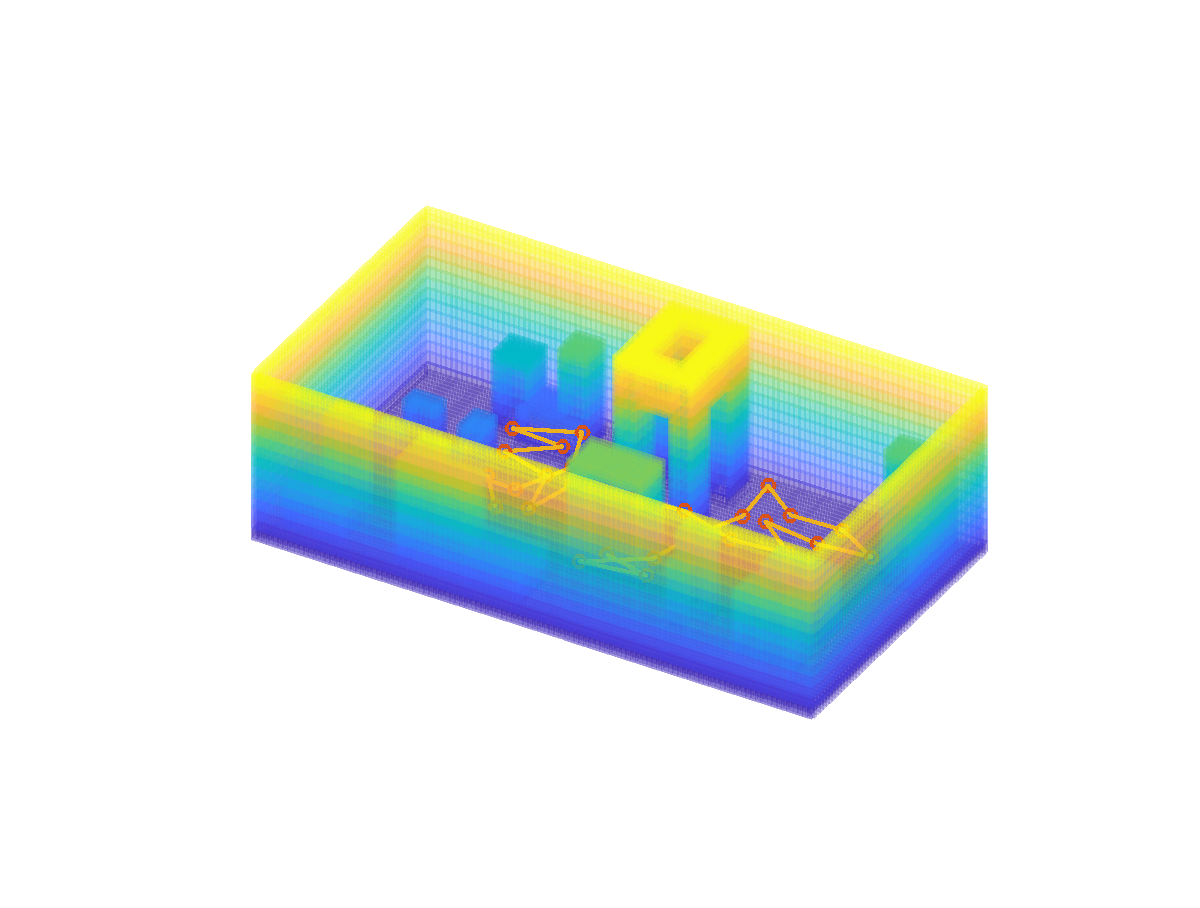
\includegraphics[trim={3.5cm 1.5cm 3cm 2.2cm}, clip = true, width = 1\textwidth]{Figs/Chapter4/search_map_1steps.eps}}
		\end{minipage}
		\begin{minipage}{.4\linewidth}
			\centering
			\subfloat[]{%
				\label{FIG:SEARCH-RESULTS-MAP-B}%
				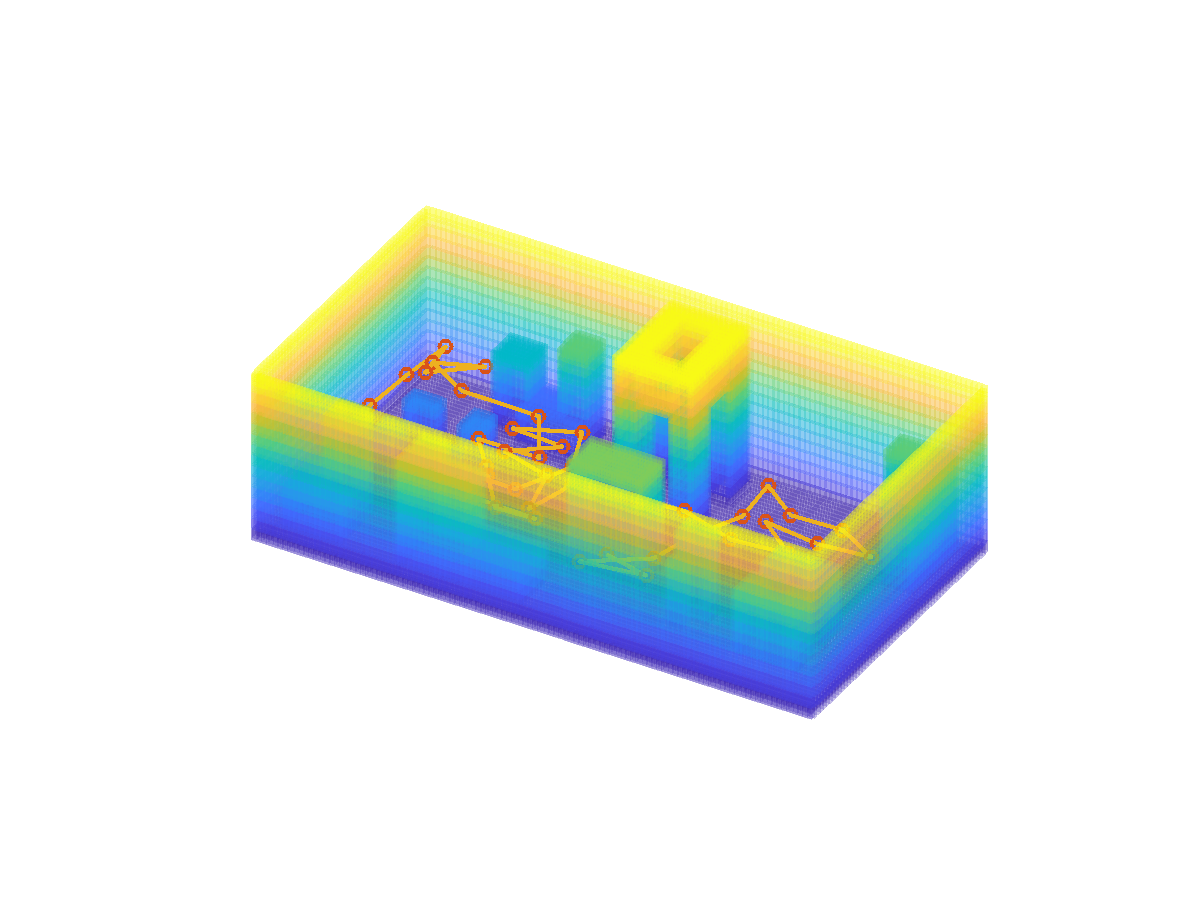
\includegraphics[trim={3.5cm 1.5cm 3cm 2.2cm}, clip = true, width = 1\textwidth]{Figs/Chapter4/search_map_2steps.eps}}
		\end{minipage}
		\begin{minipage}{.4\linewidth}
			\centering
			\subfloat[]{%
				\label{FIG:SEARCH-RESULTS-MAP-C}%
				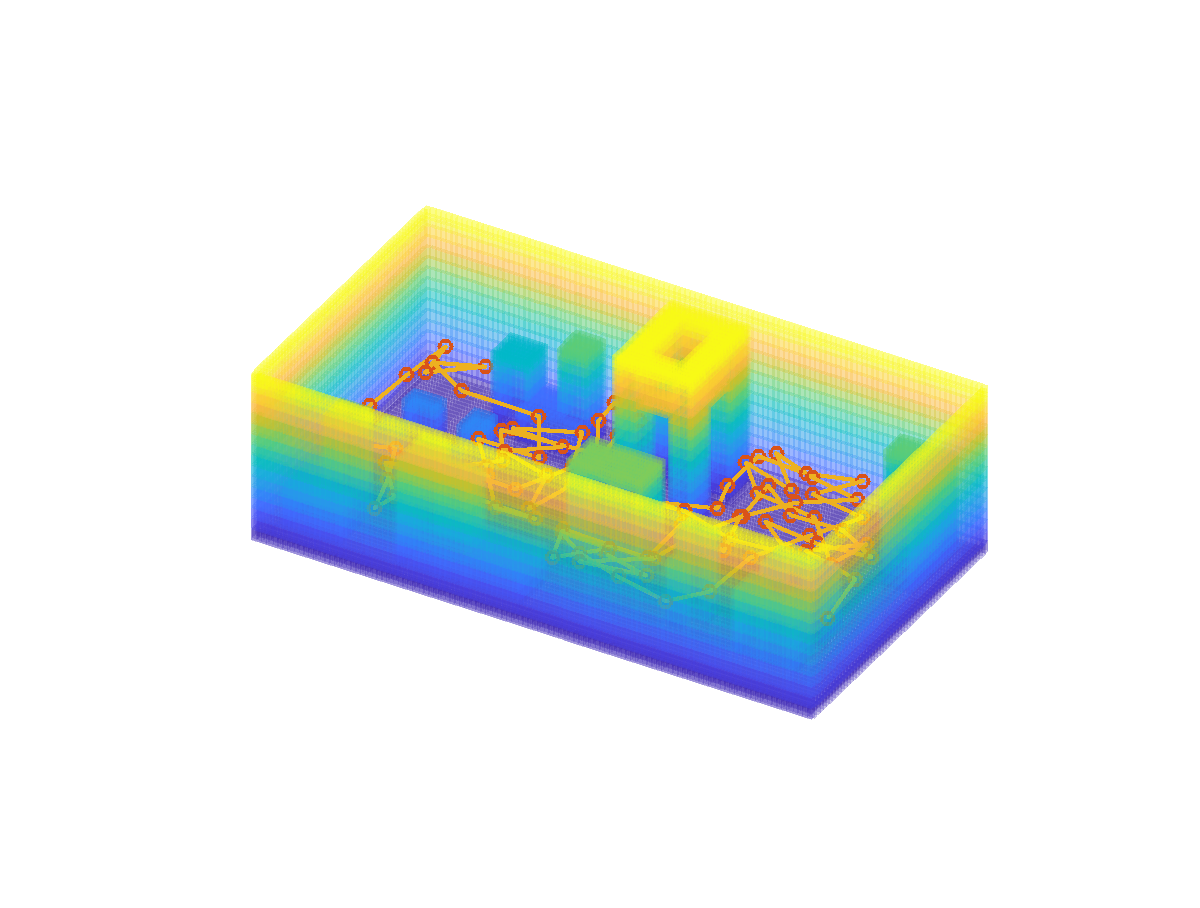
\includegraphics[trim={3.5cm 1.5cm 3cm 2.2cm}, clip = true, width = 1\textwidth]{Figs/Chapter4/search_map_5steps.eps}}
		\end{minipage}
	\end{center}
	\caption{Results of the proposed search algorithm. The figure depicts the simulated environment along with the built
	tree of possible viewpoints. Red circles represent the tree nodes, while the yellow connecting lines its edges.
	In the image, in order, (a) exploration state after only one step, (b) after two steps, and (c) after five steps.
	Note how the tree grows toward previously unexplored areas.}\label{FIG:SEARCH-RESULTS-MAP}
\end{figure}
%%%%%%%%%%
The proposed approach has been tested on a synthetic urban canyon scenario, similar to the one proposed during the Leonardo drone
contest during the third year (see~\secref{SEC:DRONE-CONTEST}). In this scenario, the $10 \times 20 \times 3$ meters map was already completely
known in advance and the flying agent was required to find as fast as possible a single moving unmanned ground robot. Thanks to these experiment
settings the explorer was initialized with a prior guess of probability distribution that equalizes to zero near and over the known
obstacles. The obtained results are reported in~\figref{FIG:SEARCH-RESULTS-MAP},~\ref{FIG:SEARCH-RESULTS-TRAJECTORY}, and~\ref{FIG:SEARCH-RESULTS-COST}.
In particular,~\figref{FIG:SEARCH-RESULTS-MAP} depicts the built tree, where red circles represent nodes and the yellow connecting lines the
tree edges, along with a discrete representation of the environment map. Overlapping~\figref{FIG:SEARCH-RESULTS-MAP} with~\figref{FIG:SEARCH-RESULTS-TRAJECTORY}
the blue continuous line represents the final trajectory followed by the drone during the exploration task. Finally,~\figref{FIG:SEARCH-RESULTS-COST}
reports the used probability map. In all the figures, in order, has been depicted the exploration state after one, two, and five steps.
Note how the agent tends to explore quickly previously unseen areas, while the probability increases over time in not visited areas and
decreases a lot after one agent visit. The proposed solution has been successfully employed during the Leonardo challenge, where
the drone was able to find out the ground agent in almost a couple of minutes, with a maximum velocity of $0.5m/s$ and starting always
from random initial positions. The algorithm was able to run completely real-time with only onboard computation and sensing capabilities.
For a complete list of the used parameters, please refer to~\tabref{TAB:SEARCH-PARAMETERS}.

In this section, we proposed a novel solution to the exploration problem in the setting where target search is the only final goal.
This approach is in contrast with the one described in~\secref{SEC:EXPLORATION-LARGE-SCALE} under different aspects, first it plans paths
instead of directly flyable trajectories, this approach may lead to degraded performances in all those cases in which the environment
is not a priori known, constraining the agent to perform several stops before starting a new exploration step. On the other hand, the latter
solution allows for continuous mapping of the target probability, which is constantly kept updated during the tree expansion.
Future research directions in this field may aim to fill the gap between these two solutions and try to solve both the problem of
environment exploration and target finding concurrently. At the same time, we wish to import the local-global paradigm even in this
class of problems, which currently is not considered yet.
%%%%%%%%%%
\begin{figure}[!t]
	\begin{center}
		\begin{minipage}{.4\linewidth}
			\centering
			\subfloat[]{%
				\label{FIG:SEARCH-RESULTS-TRAJECTORY-A}%
				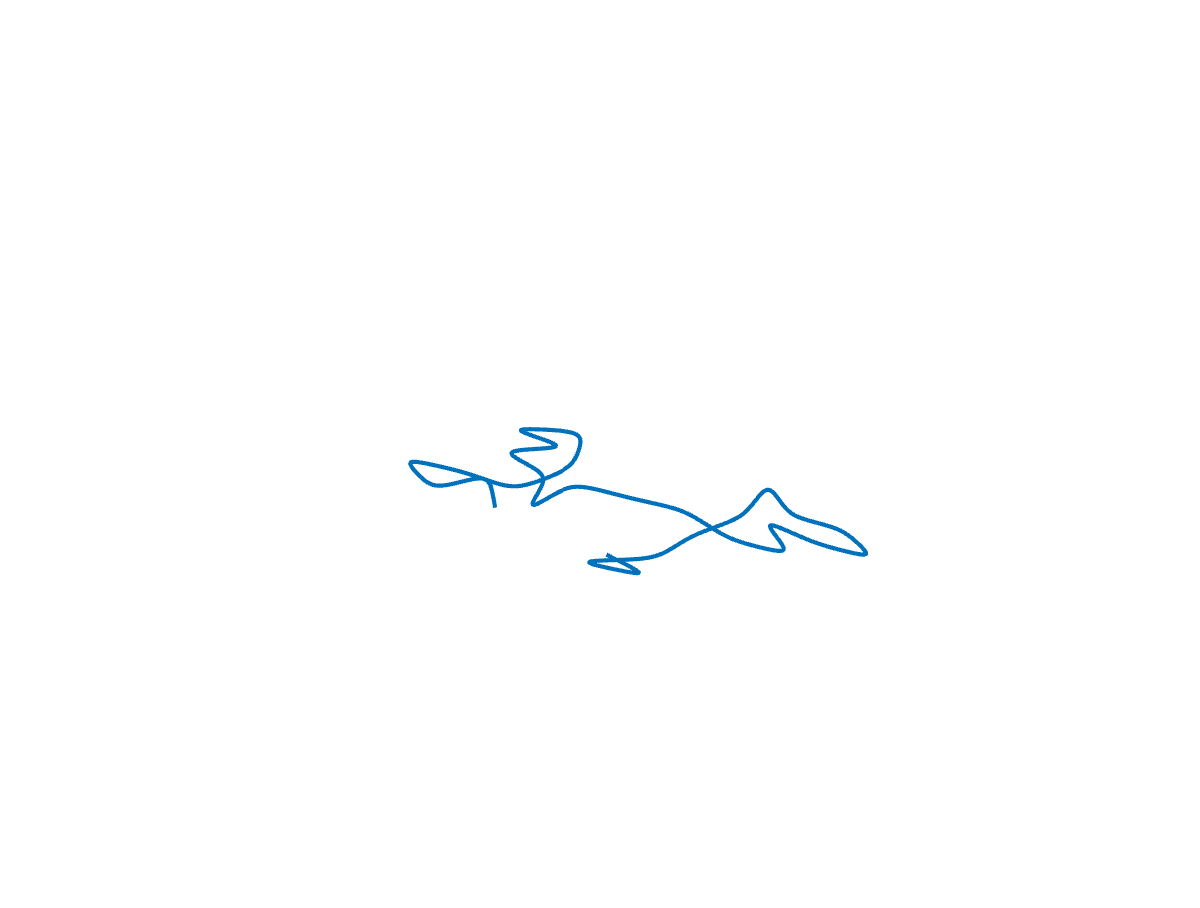
\includegraphics[trim={3.5cm 3cm 3cm 4cm}, clip = true, width = 1\textwidth]{Figs/Chapter4/search_traj_1steps.eps}}
		\end{minipage}
		\begin{minipage}{.4\linewidth}
			\centering
			\subfloat[]{%
				\label{FIG:SEARCH-RESULTS-TRAJECTORY-B}%
				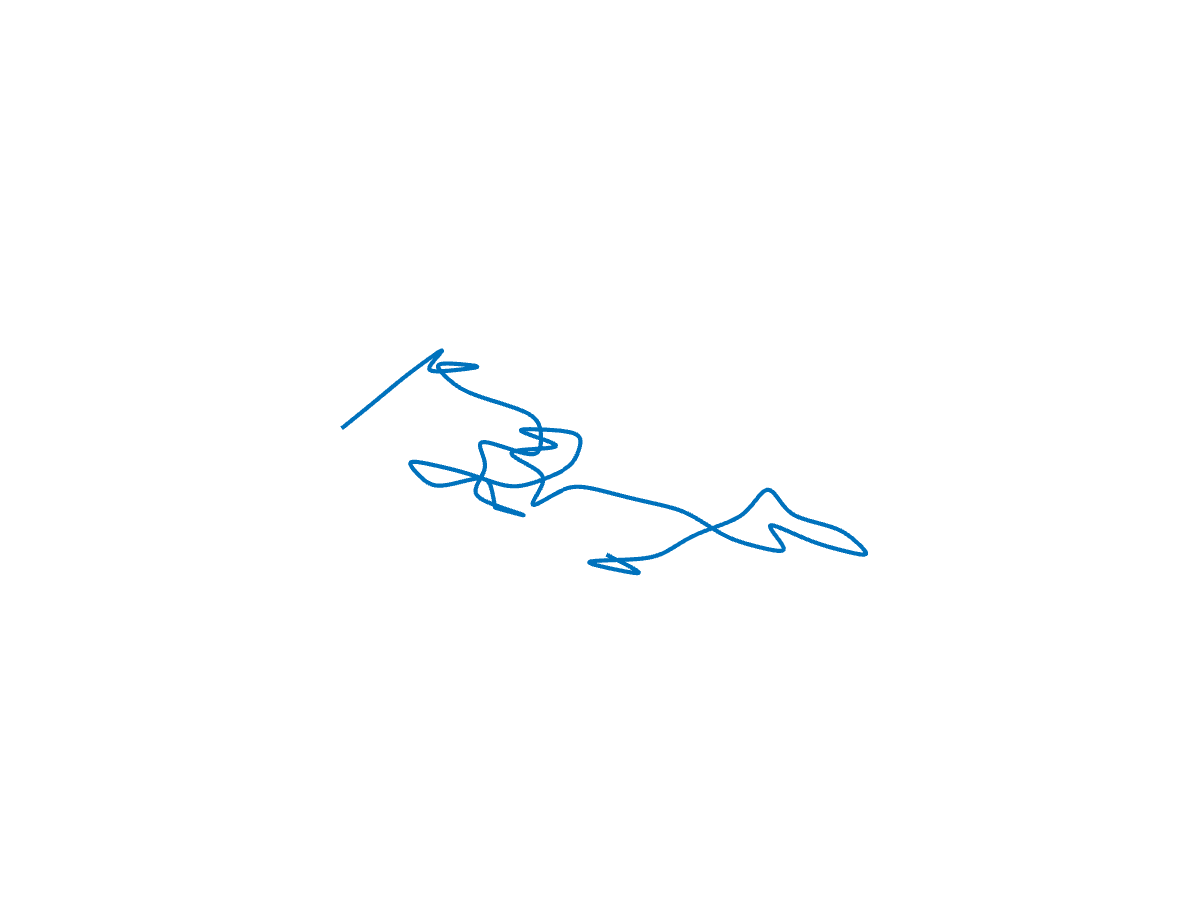
\includegraphics[trim={3.5cm 3cm 3cm 4cm}, clip = true, width = 1\textwidth]{Figs/Chapter4/search_traj_2steps.eps}}
		\end{minipage}
		\begin{minipage}{.4\linewidth}
			\centering
			\subfloat[]{%
				\label{FIG:SEARCH-RESULTS-TRAJECTORY-C}%
				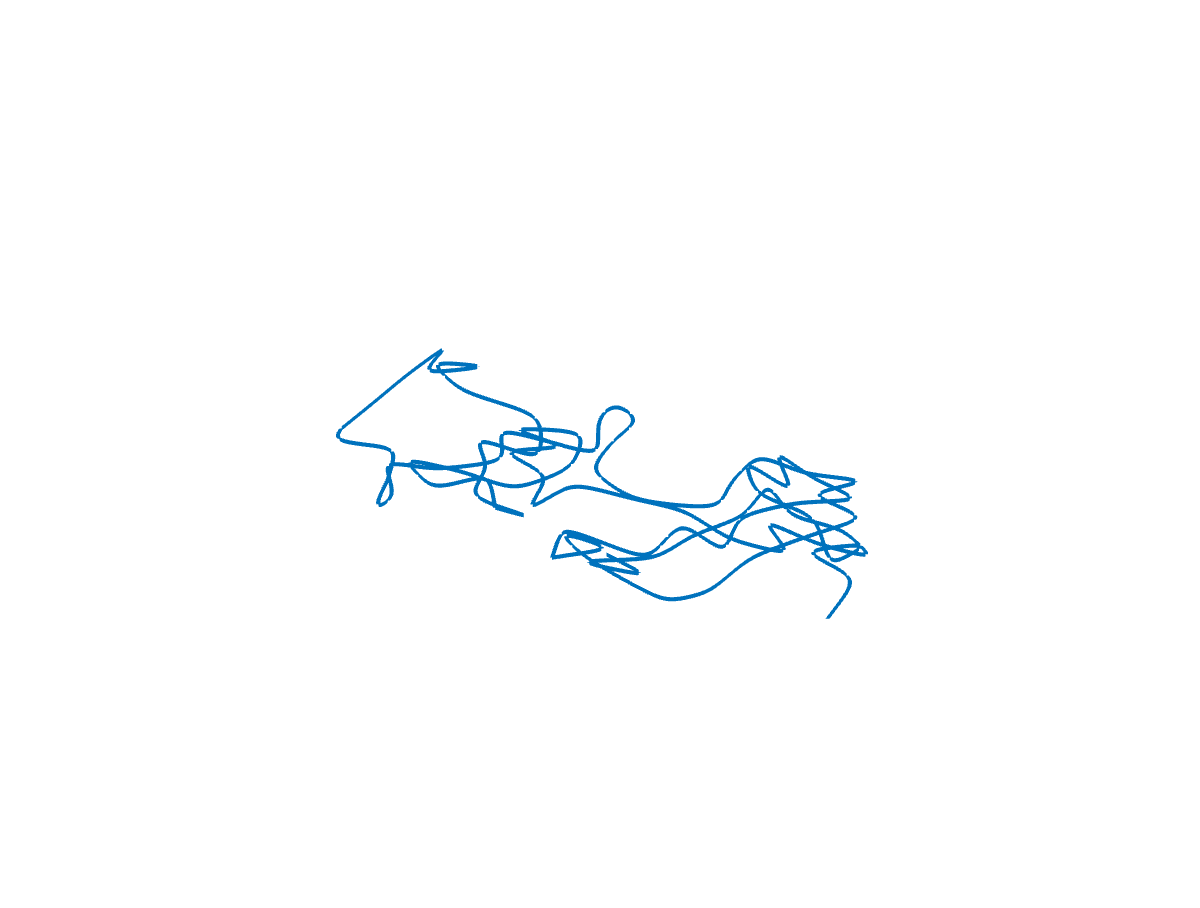
\includegraphics[trim={3.5cm 3cm 3cm 4cm}, clip = true, width = 1\textwidth]{Figs/Chapter4/search_traj_5steps.eps}}
		\end{minipage}
	\end{center}
	\caption{Results of the proposed search algorithm. The figure depicts the planned reference trajectory after (a) one exploration step,
	(b) two exploration steps, and (c) five exploration steps. The reported trajectory is built on top of the viewpoints tree reported
	in~\figref{FIG:SEARCH-RESULTS-MAP}.}\label{FIG:SEARCH-RESULTS-TRAJECTORY}
\end{figure}
%%%%%%%%%%
%%%%%%%%%%
\begin{figure}[!t]
	\begin{center}
		\begin{minipage}{.4\linewidth}
			\centering
			\subfloat[]{%
				\label{FIG:SEARCH-RESULTS-COST-A}%
				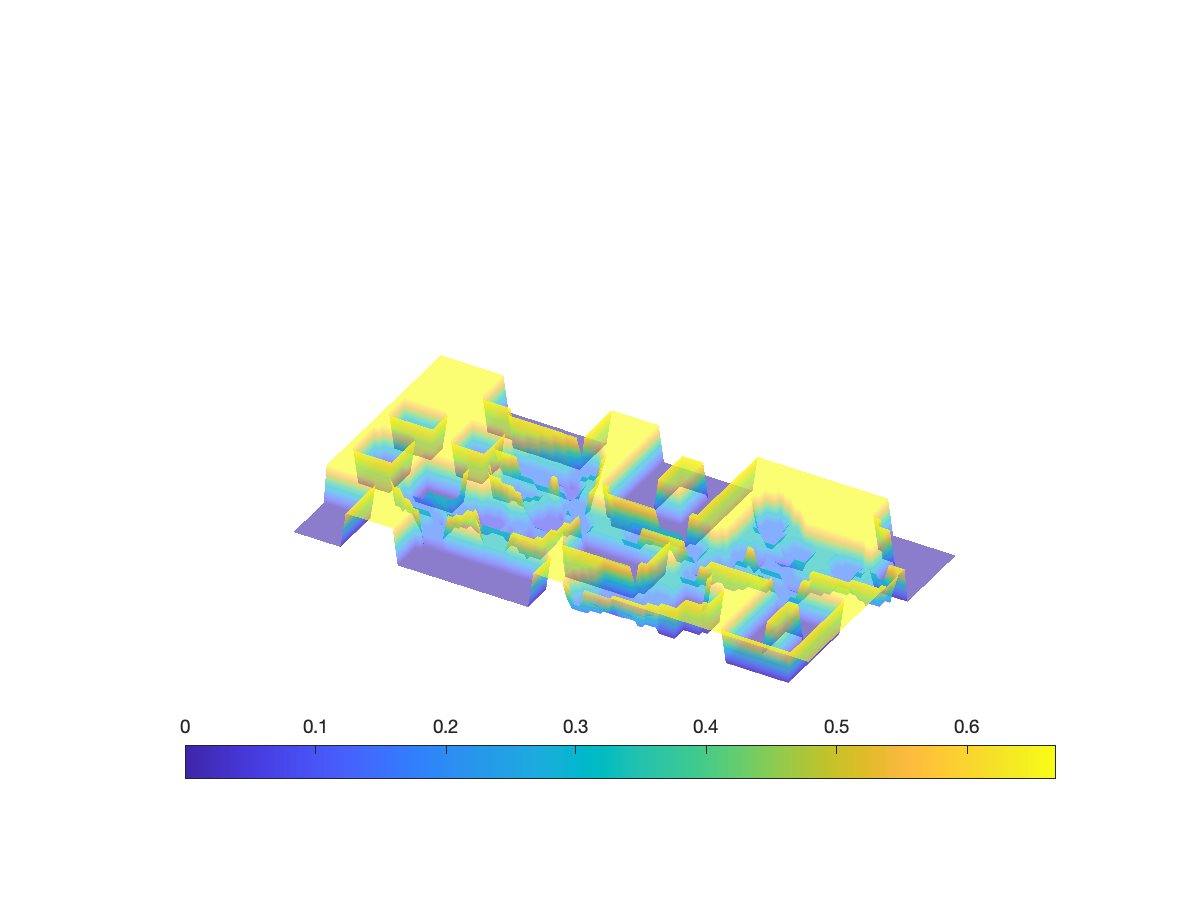
\includegraphics[trim={3.5cm 1.5cm 2cm 4cm}, clip = true, width = 1\textwidth]{Figs/Chapter4/search_cost_1steps.eps}}
		\end{minipage}
		\begin{minipage}{.4\linewidth}
			\centering
			\subfloat[]{%
				\label{FIG:SEARCH-RESULTS-COST-B}%
				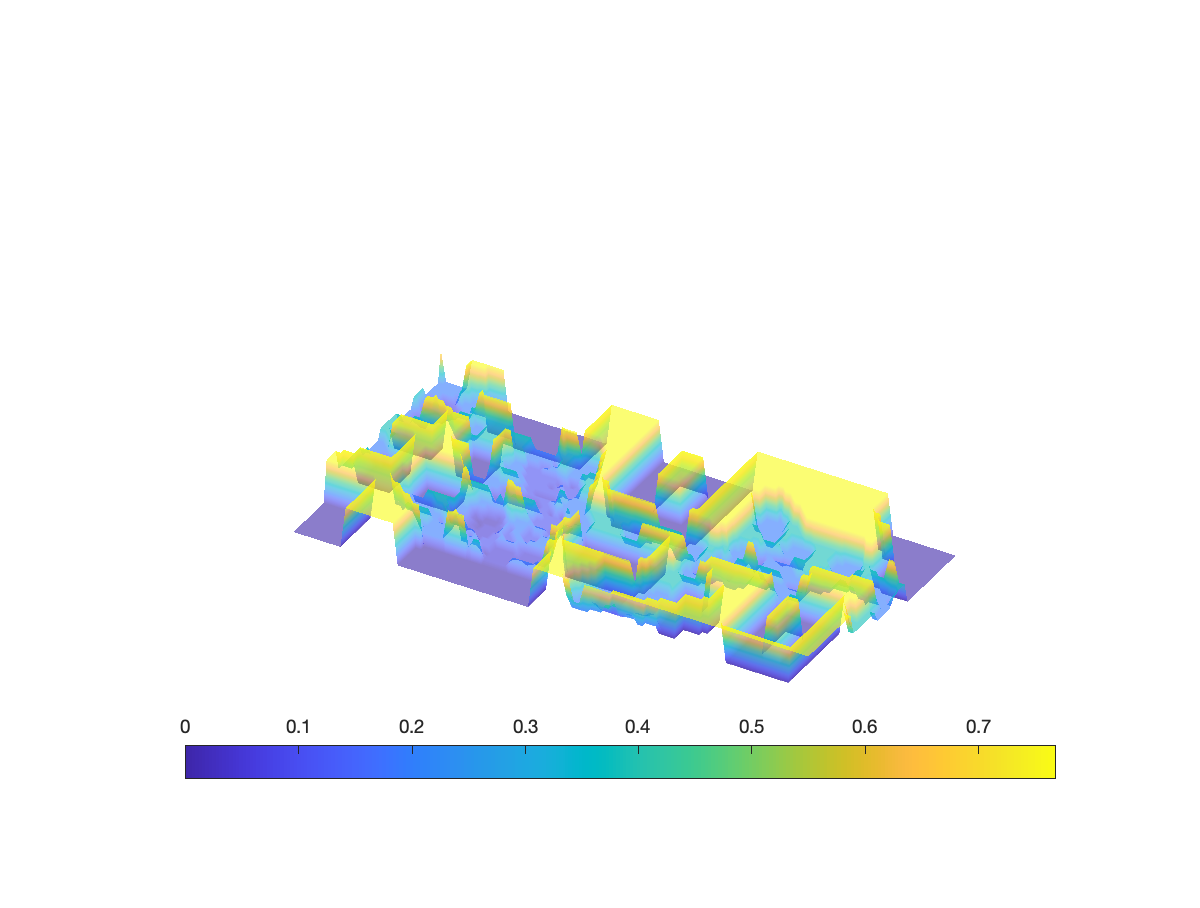
\includegraphics[trim={3.5cm 1.5cm 2cm 4cm}, clip = true, width = 1\textwidth]{Figs/Chapter4/search_cost_2steps.eps}}
		\end{minipage}
		\begin{minipage}{.4\linewidth}
			\centering
			\subfloat[]{%
				\label{FIG:SEARCH-RESULTS-COST-C}%
				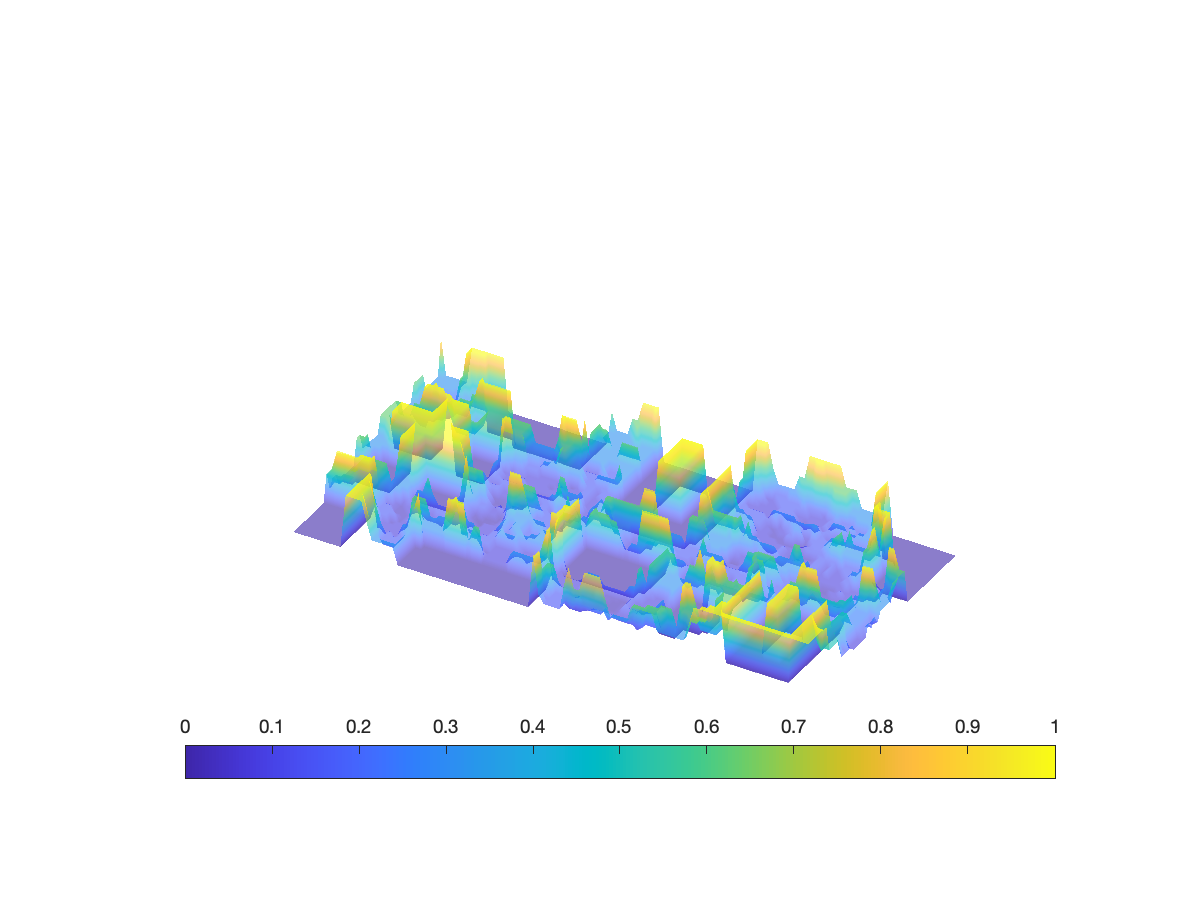
\includegraphics[trim={3.5cm 1.5cm 2cm 4cm}, clip = true, width = 1\textwidth]{Figs/Chapter4/search_cost_5steps.eps}}
		\end{minipage}
	\end{center}
	\caption{Results of the proposed search algorithm. The figure depicts the costmap state during the searching task after
	(a) one exploration step, (b) two exploration steps, and (c) five exploration steps.
	The reported costmap is used to build the tree of possible viewpoints reported in~\figref{FIG:SEARCH-RESULTS-MAP}.
	Note how the cost decreases a lot after each agent visit, how it increases in time in not visited areas, and how the cost
	is almost zero on obstacle cells. The latter property can be easily integrated into the algorithm thanks to its flexibility to
	apriori knowledge about probability distributions.}\label{FIG:SEARCH-RESULTS-COST}
\end{figure}
%%%%%%%%%%
%%%%%%%%%
{
\renewcommand{\arraystretch}{1.35}
\begin{table}[b!]
    \centering
    \begin{tabular}{||c|c||c|c||}
        \hline
        \hline
        $n_{\text{max}}$ & $1500$ & $n_{\text{sample}}$ & $60$ \\
        \hline
        $R_{\text{min}}$ & $0.5m$ & $R_{\text{max}}$ & $4.0m$ \\
        \hline
        $v_{\text{max}}$ & $0.5m/s$ & $a_{\text{max}}$ & $0.5 m/s^2$ \\
        \hline
        $p^{\text{inc}}$ & $1.01$ & $p_{\text{max}}^{\text{dec}}$ & $0.5$ \\
		\hline
		$W$ & $\lps 5, 0; 0, 5 \rps$ & $c$ & $0.0$ \\
		\hline
		$\lambda_1$ & $1.0$ & $\lambda_2$ & $10.0$ \\
        \hline
        \hline
    \end{tabular}
    \caption{Parameters used to test the object search algorithm.}%
	\label{TAB:SEARCH-PARAMETERS}
\end{table}}
%%%%%%%%%

%----------------------------------------------------------------------------------------
\section{Contributions}
This chapter is devoted to reviewing two original approaches to the problem of rapid exploration in two different contexts.
In the first stage, the focus is on the robot's capabilities and the employed algorithm is meant to carry out the exploration task
as fast as possible pushing the drone on the boundaries of its dynamical limits. While in the second stage, the focus is on the
exploration for target search. In this second case, the proposed solution mixes a continuous mapping paradigm with the random
nature of RRTs. It results in two approaches able to sequentially build high informative trajectories, or paths, in unknown, partially
known or completely known environments. In both cases, Gaussian processes have been used to fast infer the node's information gain, and
both approaches have been validated with real scenario tests. As previously mentioned, we propose, as future work to bridge the gap
between these two solutions and try to solve both the problems of environment exploration and target searching concurrently, by
planning directly sub-optimal and feasible trajectories.
We believe that the introduction of these solutions opens a new research frontier able to cope with the gap between the learning theory,
from supervised to unsupervised techniques, and the robotic world, where the limited computational power does not allows for
online network training or big data processing.

%------------------------------------------------
\chapter{Trajectory Planning}%
\label{CH:PLANNING}

%----------------------------------------------------------------------------------------
\section{The Framework}
In the previous chapter, we tracked the problem of autonomous environment \emph{exploration} from a very practical point of view,
providing a couple of possible solutions to efficiently compute high informative trajectories. Here, we moved to a slightly different
problem as the environment to navigate is completely known and the main objective is to move the autonomous agent from an initial
position, to a final one, without getting in collision with the mapped obstacles and without the necessity to gather information about
the surroundings. In these settings, the planned trajectory is required only to be \emph{safe} in the sense that does not collide with
any obstacles and develops inside known and free environment areas, and to fully satisfy the agent dynamical capabilities.
As the trajectory is not meant to gather as much data as possible, it can be designed to optimise whatever user-defined loss function,
from the overall travel time, to control effort, or high derivatives. In the Leonardo drone contest case, a trajectory planning module
was required to navigate the environment and reach a goal position smoothly and quickly, so the quadrotor is steered in a way that
the localisation and the collision avoidance (see later in~\chref{CH:AVOIDANCE}) parts can work as well as possible.

In this chapter, after a brief literature review, we analyze and adapt a state-of-the-art solution to the trajectory planning problem.
The proposed solution has been successfully implemented and deployed during the Leonardo drone contest.
For further details the reader is referred to the original work~\cite{zhou2019robust}.

\subsection{Related Works}
Although the literature is cluttered with possible solutions to the problem of trajectory planning, most of them can be classified
solely into two categories: \emph{hard-constrained} and \emph{soft-constrained} methods.
Hard-constrained methods reformulate the planning problem as a convex optimisation one, where collisions are avoided by constraining
the planned path to be inside a set of convex flight corridors.
This idea was pioneered by~\cite{mellinger2011minimum} who proposes to generate minimum-snap trajectories
via Quadratic Programming (QP) approach, and by~\cite{richter2016polynomial} who, in turn, presented a closed-form approach
to the minimum-snap trajectory generation problem.
Both the latter approaches parametrise the overall trajectory as $n$-segments piecewise polynomial curve,
and ensure the trajectory safety by iteratively adding intermediate waypoints.
Similar approaches generate safe trajectories via convex optimisation~\cite{chen2015real, gao2016online, liu2017planning, ding2018trajectory, ding2019efficient, gao2018online},
but, unlike the pioneer solutions, here the problem is solved in a two-steps pipeline. First, a sequence of cubes~\cite{gao2018online},
spheres~\cite{gao2019flying}, or polyhedrons~\cite{liu2017planning}, are fitted inside the free and navigable space, then the
reconstructed flight corridors are used as convex constraints inside the optimisation problem.
The works of~\cite{ding2018trajectory, ding2019efficient} proposed a B-Spline-based search able to generate trajectories used as 
an initial guess for the subsequent optimisation step.
Thanks to the convex reformulation, hard-constrained methods guarantee global optimality at the expense of all possible nonconvex
costs and constraints, such as distance from obstacles and conservative kinodynamic constraints, leading often to unsafe and
conservative paths.
On the other hand, soft-constrained methods reformulate trajectory planning as a non-linear optimisation problem able to keep
smoothness, feasibility, and safety into account.
In~\cite{zucker2013chomp} the authors generate discrete-time trajectories minimizing both smoothness and risk of collision via
gradient descent methods, while in~\cite{kalakrishnan2011stomp} the optimisation is solved in a gradient-free fashion.
The work of~\cite{oleynikova2016continuous} extended the latter approaches to continuous-time polynomial trajectories, thanks to the
continuous-time formulation it avoids numeric differentiation errors leading to a more accurate representation.
However, the approach proposed by~\cite{oleynikova2016continuous} suffers from low success rate, being the proposed optimisation problem
solved without a good initial guess.
As a matter of fact, the success rate considerably improved when~\cite{gao2017gradient} proposes to solve the same problem
with a collision-free path used as an initial condition. The latter path is obtained via sampling-based path searching methods.
In~\cite{usenko2017real} the trajectory is parameterized as an uniform B-Spline, whose intrinsic continuity allows to reduce
the overall number of constraints.
Soft-constrained solutions make use of gradient information to push the final trajectory far from obstacles, but may suffer from
local minima and do not have any guarantee of success rate and kinodynamic feasibility.
The work of~\cite{zhou2019robust} proposes a novel soft-constrained method where the B-Spline parameterisation is used to both
speed-up the cost computation and simplify the collision checking thanks to its convex hull containment property (see~\appref{SEC:SPLINES-APPENDIX}).

%----------------------------------------------------------------------------------------
\section{Quadrotor Trajectory Generation}
In this section we review a trajectory planning approach first proposed by~\cite{zhou2019robust}.
The considered approach aims to efficiently compute minimum effort safe trajectories, balancing both the induced control effort and
the overall trajectory time. This soft-constrained approach develops in two steps, first a collision-free suboptimal trajectory
is computed via \emph{hybrid-state} A$^{\star}$ search, then the obtained solution is iteratively refined via non-linear
optimisation. In this second step the B-Spline formulation is adopted to improve the algorithm convergency rate.

\subsection{Hybrid-State A$^{\star}$}
The first step consists of raw trajectory planning via A$^{\star}$ graph search, unlike the standard A$^{\star}$ formulation, here
the proposed solution expands and optimises a graph of possible kinodynamic feasible trajectories (from this property the \emph{hybrid-state} attribute).
In this settings, the A$^{\star}$ optimisation is applied to a tree $\tree = \lp \NN, \EE \rp$ consisting of a set of nodes
$\NN = \left\{ N_1, \dots, N_{n_{N}} \right\}$ and a set of edges $\EE = \left\{ E_1, \dots, E_{n_{E}} \right\}$, where each node
is completely defined by the following six quantities
\begin{equation*}
	\NN_i = \left\{ \bs{x}_i, \bs{u}_i, \delta^t_i, \chi_i, g_i, h_i \right\},
\end{equation*}
where $\bs{x}_i$ and $\bs{u}_i$ represent the current quadrotor state and the applied input used to reach that state,
$\delta^t_i$ is the amount of time for which $\bs{u}_i$ is applied, $\chi_i$ is an unique integer indexing $\bs{x}_i$ over a voxel grid,
and $\lp g_i, h_i \rp$ are two costs associated with the current node useful for the graph optimisation, in particular $g_i$ is the
\emph{true} trajectory cost, while $h_i$ represents a heuristic estimating the cost-to-go to reach the goal state.
The graph edges are generated by motion primitives respecting the quadrotor dynamics, instead of standard straight lines.
As in~\secref{SEC:EXPLORATION-LARGE-SCALE}, here we enforce the differential flatness property commonly used in quadrotor planning,
and express the final state trajectory through the evolution of only the three axis-wise positions
so $\bs{x} = \lp p_x, p_y, p_z \rp \in \R^3$, where each component can be designed as a time-parameterized polynomial function
\begin{equation}
	\label{EQ:POLYNOMIAL-EXPANSION}
	p_j \lp t \rp = \sum_{k=0}^{n} a_kt^k.
\end{equation}
The aformentioned formulation correspond to a Linear Time-Invariant (LTI) system, letting
$\bs{z} = \lp \bs{x}\T, \bs{x}^{{\lp 1 \rp}\T}, \dots, \bs{x}^{{\lp n-1 \rp}\T} \rp\T \in \R^{3n}$  the state vector,
and $\bs{u} =  \bs{x}^{\lp n \rp} \in \mathcal{U} = \lps \bs{u}_{\text{min}}, \bs{u}_{\text{max}}\rps \subset \R^{3}$ the control input,
then the state-space model can be defined as
\begin{equation*}
	\dot{\bs{z}} = A \bs{z} + B \bs{u},
\end{equation*}
with $A \in \R^{3n \times 3n}$ and $B \in \R^{3n \times 3}$ matrices in prime form.
The complete solution for the state equation, giving the quadrotor trajectory from the initial condition $\bs{z}_0$, is expressed as
\begin{equation}
	\label{EQ:MOTION-PRIMITIVE}
	\bs{z}\lp t \rp = \exp \lp At \rp\bs{z}_0 + \int_{0}^{t} \exp \lp A \lp t-\tau \rp \rp B \bs{u}\lp \tau \rp d\tau.
\end{equation}
In these settings, a set of motion primitive, leading to a set of possible graph edges for each node, can be efficiently computed
by propagating~\eqqref{EQ:MOTION-PRIMITIVE} for a fixed time step $\delta^t$, applying a set of discretised control inputs
$\mathcal{U}_{\text{D}} \subset \mathcal{U}$. From a practical point of view, the set $\lps \bs{u}_{\text{min}}, \bs{u}_{\text{max}} \rps$
can be uniformly discretised in $r$ steps along each axis, yielding to $r^3$ possible motion primitives.
The graph search then unfolds as a classical A$^{\star}$ search, for each node a set of edges and children nodes are generated via motion
primitive propagation, then each child is checked against dynamical feasibility and possible collision with map obstacles, and only those
nodes considered as feasible are retained for future expansions.
To speed-up the search a voxel grid discretisation is imposed over the trajectory space so all children nodes whose associated index $\chi$
matches in the list of already expanded cells are culled out from the open set.

In order to let the adopted search effective, we need an admissible and informative loss formulation for both the true trajectory cost
and the estimated cost-to-go. Under this perspective, since the main trajectory planning objective is to generate motions balancing both
control effort and overall traveling time, the natural loss formulation is
\begin{equation}
	\label{EQ:PLANNING-LOSS}
	\loss = T + \rho \int_0^T \norm{\bs{u} \lp \tau \rp}^2 d \tau,
\end{equation}
where $T$ is the total trajectory time, $\bs{u}$ is the control action, and $\rho \in \R_{>0}$ is a weight coefficient balancing between
minimum time and minimum effort trajectories.
Under the loss function~\eqref{EQ:PLANNING-LOSS}, the true cost $g_i$, representing the trajectory cost form the start position, can be
computed summing up the cost of all primitives applied so far
\begin{equation*}
	g_i = g_{i-1} + \lp 1 + \rho\norm{\bs{u}_i}^2 \rp \delta_i^t.
\end{equation*}
As regards the heuristic cost-to-go $h_i$, we need an estimation of $\loss$ from the current state $\bs{x}_i$ to the goal one.
To retrieve this estimation, we compute a closed-form trajectory, from $\bs{x}_i$ to the goal state, that minimizes the cost $\loss$
by applying the Pontryagins minimum principle~\cite{mueller2015computationally}.
In particular, letting $n = 3$ in~\eqqref{EQ:POLYNOMIAL-EXPANSION}, then the optimal trajectory $p\lp t \rp$ minimising $\loss$ can
be computed as
\begin{equation}
	\label{EQ:OPTIMAL-TRAJECTORY}
	p^{\star}_{\mu} = \frac{1}{6}\alpha_{\mu}t^3 + \frac{1}{2}\beta_{\mu}t^2 + v_{\mu_0}t + p_{\mu_0} \hspace*{0.5cm} \text{with } \mu = x,y,z,
\end{equation}
where the parameters $\alpha_{\mu}$ and $\beta_{\mu}$ follow the relation
\begin{equation*}
	\begin{pmatrix}
		\alpha_{mu} \\ \beta_{\mu}
	\end{pmatrix} = \frac{1}{T^{{\star}^3}}
	\begin{pmatrix}
		-12 & 6T^{\star} \\ 6T^{\star} & -12T^{{\star}^2}
	\end{pmatrix}
	\begin{pmatrix}
		p_{\mu_{\text{goal}}} - p_{\mu_0} - v_{\mu_{\text{goal}}}T^{\star} \\
		v_{\mu_{\text{goal}}} - v_{\mu_{0}}
	\end{pmatrix},
\end{equation*}
and $p_{\mu_0}$, $p_{\mu_{\text{goal}}}$, $v_{\mu_0}$, and $v_{\mu_{\text{goal}}}$ represent the initial and goal position and velocity, respectively.
The optimal time $T^{\star}$ can be compute by deriving~\eqqref{EQ:OPTIMAL-TRAJECTORY} and plugging it inside~\eqqref{EQ:PLANNING-LOSS}
\begin{equation*}
	T^{\star} = \argmin_{T > 0} \sum_{\mu \in \{ x,y,z \}} \frac{1}{3} \alpha_{\mu}^2T^3 + \alpha_{\mu}\beta{\mu}T^2 + \beta_{\mu}^2T.
\end{equation*}
The optimal cost $\loss^{\star} = \loss \lp p^{\star}, T^{\star}\rp$ is then used in place of $h_i$ as cost-to-go estimation.
\begin{remark}
	The choice $n = 3$ leads to \emph{minimum jerk} trajectories as the control action $\bs{u} = \bs{x}^{\lp 3 \rp}$. 
\end{remark}
\begin{remark}
	The computed optimal trajectory $p^{\star}$ contributes to the planning procedure more than only providing an admissible heuristic.
	As a matter of fact, $p^{\star}$ is useful twice as it can be used to stop the search in advance, provided that the computed trajectory
	satisfies all dynamical and collision constraints. Moreover, such an analytic expansion is of fundamental importance as, due to the
	control discretisation, it is difficult to have a primitive end exactly in the goal state.
\end{remark}

\subsection{B-Spline Trajectory Optimisation}
The second step of the proposed trajectory planning method consists of a trajectory optimisation procedure.
This step is fundamental in smoothing the initial trajectory produced by the path searcher, which is suboptimal due to the control discretisation,
and to push the final trajectory away from the obstacles, since the distance information in the free space is ignored at search time.
Here, as in~\secref{SEC:SEARCH-TRAJECTORY-OPTIMISATION}, to speed-up the solver and improve the planner success rate, we enforce the use of
B-Spline curves (see~\secref{SEC:SPLINES-APPENDIX}) as time parameterisation for the quadrotor trajectory.
As already mentioned in~\secref{SEC:SEARCH-TRAJECTORY-OPTIMISATION}, B-splines are defined by a set of control points
$\CP = \lps \bs{\cpoint}_0, \dots, \bs{\cpoint}_{\cpnumber} \rps$, and a set of time knots
$\bs{\splinevar} = \lps \splinevar_0, \dots, \splinevar_{\cpnumber + \order + 1} \rps$, as
\begin{equation*}
	\bs{\spline} \lp \splinevar \rp = \sum_{i=0}^\cpnumber \basis_i^\order \lp \splinevar \rp \bs{\cpoint}_i,
\end{equation*}
with $\order$ order of the spline and $\basis_i^\order$ basis functions, recursively computed via the De-Boor formula~\cite{de1978practical}.
The use of B-Spline in trajectory optimisation is attractive thanks to its convex hull containment property, which allows approximating
the collision condition of the overall trajectory by directly conditioning its control points $\CP$ lying to a free non-necessary convex
environment area. Moreover, by evaluating the control points distance from the obstacles we can directly assess the trajectory safeness.
Another useful property is represented by the closure with respect to integration and derivation, so the derivatives $\bs{\spline}^{\lp d \rp}$
of a B-Spline still maintain a B-Spline structure with control points
\begin{equation*}
	\bs{\cpoint}_i^{\lp d \rp} = \order \frac{\bs{\cpoint}_{i+1}^{\lp d-1 \rp} - \bs{\cpoint}_i^{\lp d-1 \rp}}{\splinevar^{\lp d-1 \rp}_{i+\order+1} - \splinevar^{\lp d-1 \rp}_{i+1}}.
\end{equation*}
These properties, jointly with the differential flatness one, can be used to ease the trajectory optimisation procedure as both the
collision and dynamics constraints can be refurmulated linearly in terms of the trajectory control points, which are then used as
decision variables. For this purpose, we fix an uniformly distributed knot vector of the form
\begin{equation*}
	\bs{\splinevar} =
	\begin{bmatrix}
		0_{0:7}, & \Delta_{\splinevar}, & 2\Delta_{\splinevar}, & \dots, & (\cpnumber-\order)\Delta_{\splinevar}, & T_{0:7}
	\end{bmatrix},
\end{equation*}
with $\Delta_{\splinevar} = T/(\cpnumber - \order + 1)$, and $T$ the total trajectory time computed in the search phase.
Then we formulate the trajectory optimisation step as an uncostrained optimisation problem of the form
\begin{equation}
	\label{EQ:PLANNING-OPTIMISATION}
	\min_{\bs{\cpoint}_0, \bs{\cpoint}_1, \dots, \bs{\cpoint}_{\cpnumber}} \lambda_{\text{s}} \loss_{\text{s}} + 
	\lambda_{\text{c}} \loss_{\text{c}} + \lambda_{\text{f}} \lp \loss_{\text{v}} + \loss_{\text{a}} \rp,
\end{equation}
where $\lambda_{\text{s}} \in \R_{<0}$, $\lambda_{\text{c}} \in \R_{<0}$, and $\lambda_{\text{f}} \in \R_{<0}$ are
weight coefficients balacing between trajectory smoothness $\loss_{\text{s}}$, distance from obstacles $\loss_{\text{c}}$,
velocity feasibility $\loss_{\text{v}}$, and acceleration feasibility $\loss_{\text{a}}$.
Each cost is formulated taking into account the B-Spline parameterisation and properties.
The smoothness cost $\loss_{\text{s}}$ tries to pursue the same goal carried out by the searcher to minimise the overall control
effort, thus with $n = 3$, $\loss_{\text{s}}$ reads to
\begin{equation*}
	\loss_{\text{s}} = \int_0^{T} \norm{\frac{d^n \bs{\spline} \lp \splinevar \rp}{d \splinevar^n}}^2 d \splinevar,
\end{equation*}
which can be computed in closed form for B-Spline parameterisation (see~\secref{SEC:SPLINES-APPENDIX}).
The collision cost $\loss_{\text{c}}$ is formulated as the repulsive force of the obstacles acting on each control point
\begin{equation*}
	\loss_{\text{c}} = \sum_{i = 0}^{\cpnumber}
	\begin{cases}
		\begin{matrix}
			\lp d \lp \bs{\cpoint}_i \rp - d_{\text{thr}} \rp^2 & d \lp \bs{\cpoint}_i \rp \le d_{\text{thr}}, \\
			0 & d \lp \bs{\cpoint}_i \rp > d_{\text{thr}},
		\end{matrix}
	\end{cases}
\end{equation*}
where $d \lp \bs{\cpoint}_i \rp$ is the distance of $\bs{\cpoint}_i$ from the closer mapped obstacle, and $d_{\text{thr}}$
is a minimum distance considered as \emph{safe}.
Finally the velocity and acceleration feasibility cost is formulated as
\begin{equation*}
	\loss_{\text{v}} = \sum_{\mu = \{ x,y,z \}} \sum_{i = 0}^{\cpnumber - 1}
	\begin{cases}
		\begin{matrix}
			\lp \bs{\cpoint}_i^{{\lp 1 \rp}^2} - v_{\text{max}}^2 \rp^2 & \bs{\cpoint}_i^{{\lp 1 \rp}^2} \le v_{\text{max}}^2, \\
			0 & \bs{\cpoint}_i^{{\lp 1 \rp}^2} < v_{\text{max}}^2,
		\end{matrix}
	\end{cases}
\end{equation*}
\begin{equation*}
	\loss_{\text{a}} = \sum_{\mu = \{ x,y,z \}} \sum_{i = 0}^{\cpnumber - 2}
	\begin{cases}
		\begin{matrix}
			\lp \bs{\cpoint}_i^{{\lp 2 \rp}^2} - a_{\text{max}}^2 \rp^2 & \bs{\cpoint}_i^{{\lp 2 \rp}^2} \le a_{\text{max}}^2, \\
			0 & \bs{\cpoint}_i^{{\lp 2 \rp}^2} < a_{\text{max}}^2,
		\end{matrix}
	\end{cases}
\end{equation*}
where $v_{\text{max}}$ and $a_{\text{max}}$ are the axis-wise maximum velocity and acceleration, respectively.
\begin{remark}
	The problem~\eqref{EQ:PLANNING-OPTIMISATION} does not ensure neither safety, nor dynamical feasibility as the constraints
	has been softly injected inside the cost. Nevertheless, there exists a local optimal close to the initial trajectory planned by
	the searcher, so the problem~\eqref{EQ:PLANNING-OPTIMISATION} quickly converges to the local optimal solution if initialised with a
	good and feasible initial condition.
\end{remark}

\subsection{Experimental Results}
\begin{figure}[!t]
	\begin{center}
		\begin{minipage}{.45\linewidth}
			\centering
			\subfloat[]{%
				\label{FIG:PLANNING-RESULTS-MAP-TRAJECTORY-A}%
				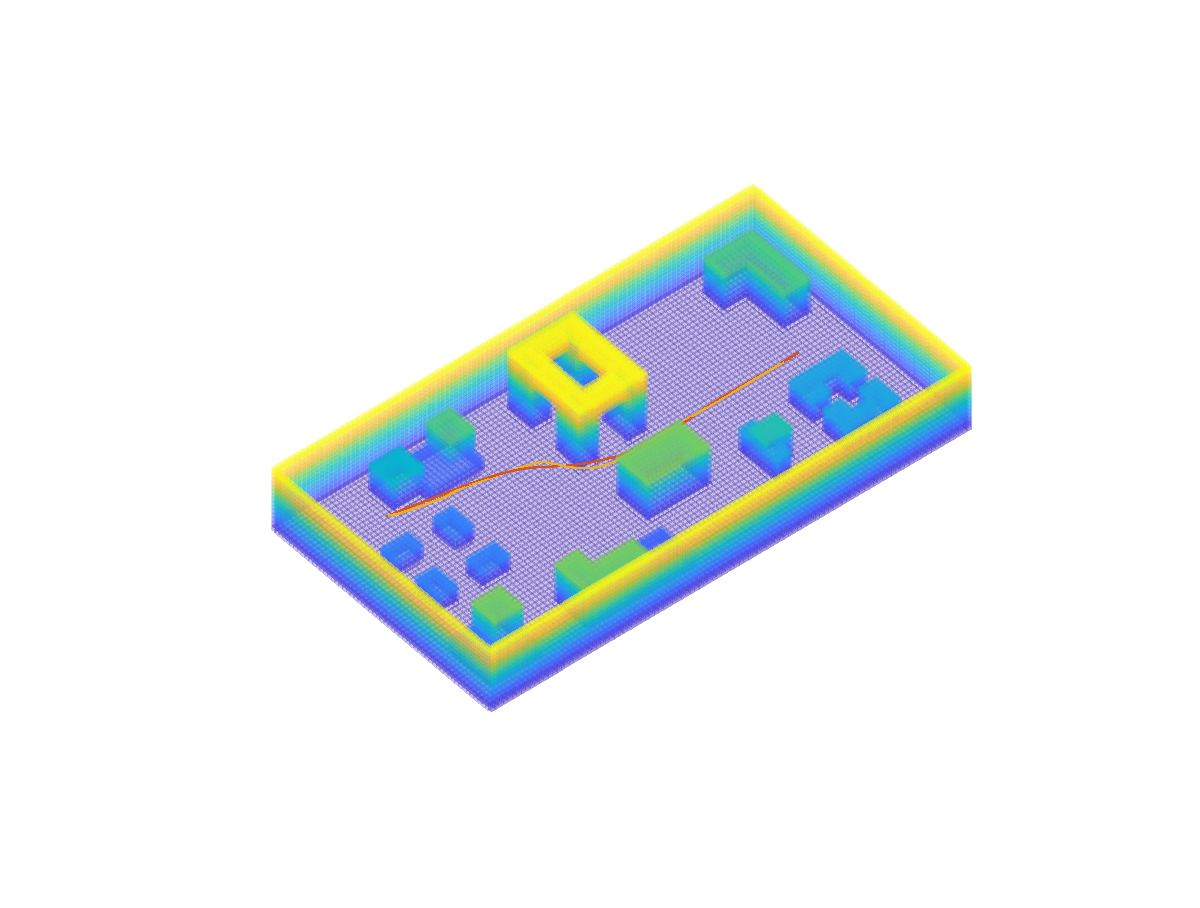
\includegraphics[trim={3.5cm 2.5cm 3cm 2.5cm}, clip = true, width = 1.05\textwidth]{Figs/Chapter5/planning-full.eps}}
		\end{minipage}
		\begin{minipage}{.45\linewidth}
			\centering
			\subfloat[]{%
				\label{FIG:PLANNING-RESULTS-MAP-TRAJECTORY-B}%
				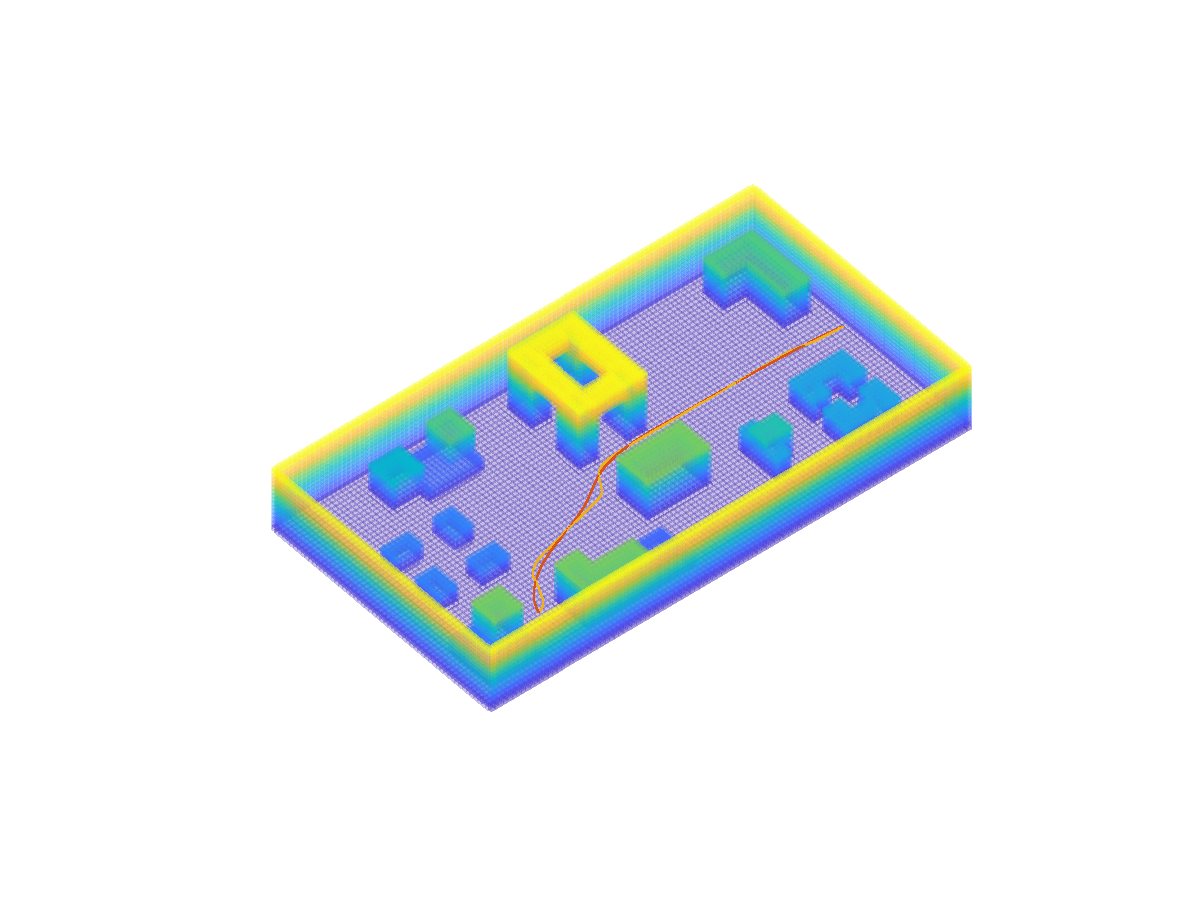
\includegraphics[trim={3.5cm 2.5cm 3cm 2.5cm}, clip = true, width = 1.05\textwidth]{Figs/Chapter5/planning-full-2.eps}}
		\end{minipage}
	\end{center}
	\caption{Results of the proposed trajectory planning algorithm. The figure depicts the simulated environment along with the planned
	trajectory by the searcher (yellow line), and the output of the trajectory optimisation step (red line). Notice how the optimised
	trajectory smoothly follows the yellow path without colliding with the environment obstacles.}%
    \label{FIG:PLANNING-RESULTS-MAP-TRAJECTORY}
\end{figure}
\begin{figure}[!t]
	\begin{center}
		\begin{minipage}{.45\linewidth}
			\centering
			\subfloat[]{%
				\label{FIG:PLANNING-RESULTS-TRAJECTORY-A}%
				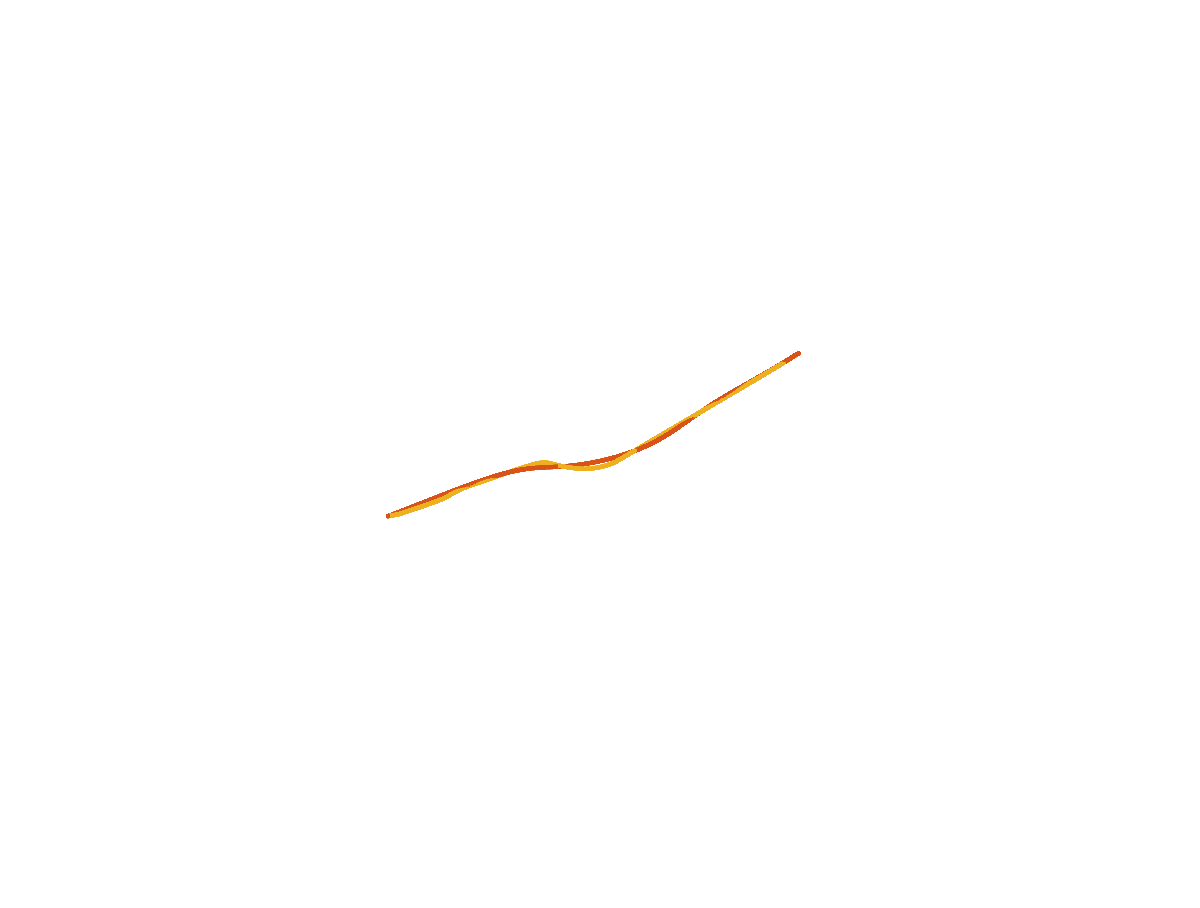
\includegraphics[trim={3.5cm 2.5cm 3cm 2.5cm}, clip = true, width = 1.05\textwidth]{Figs/Chapter5/planning-traj.eps}}
		\end{minipage}
		\begin{minipage}{.45\linewidth}
			\centering
			\subfloat[]{%
				\label{FIG:PLANNING-RESULTS-TRAJECTORY-B}%
				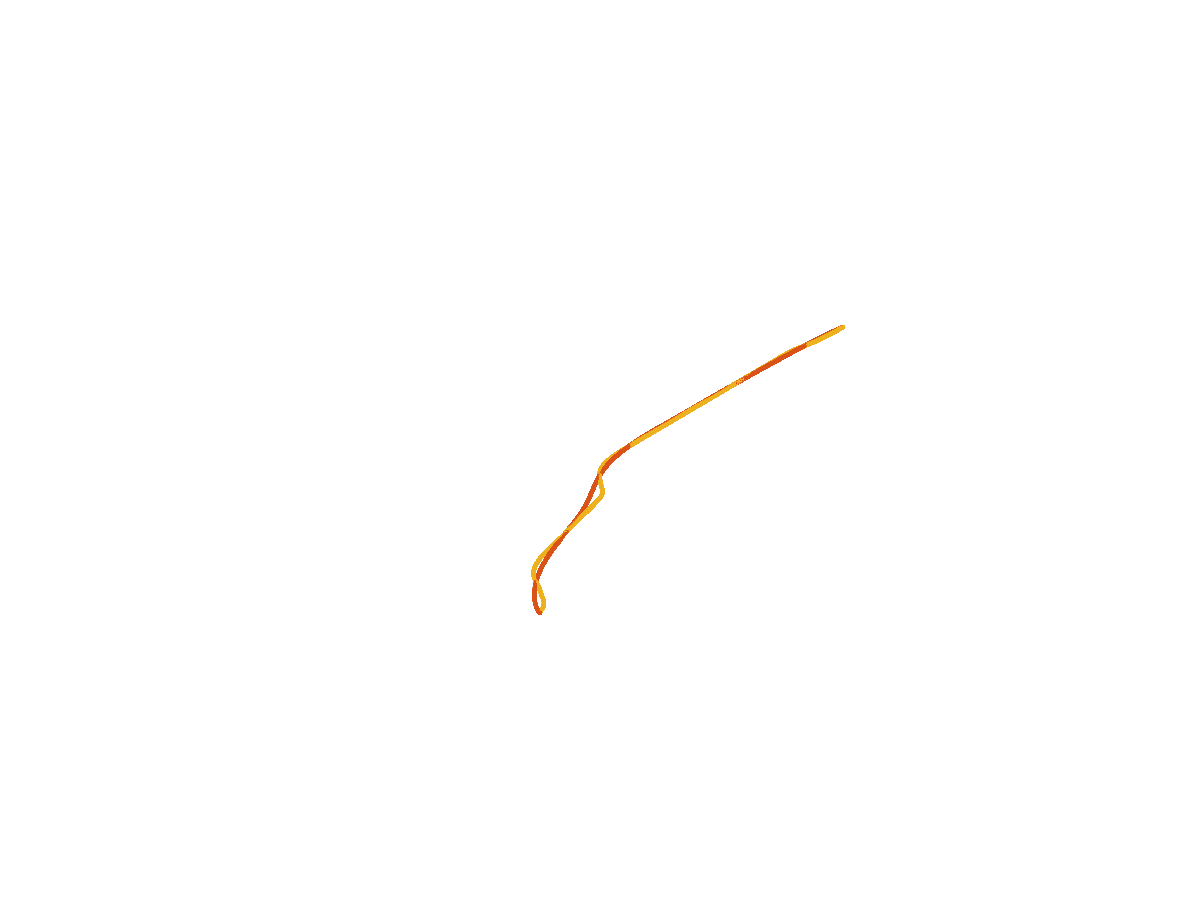
\includegraphics[trim={3.5cm 2.5cm 3cm 2.5cm}, clip = true, width = 1.05\textwidth]{Figs/Chapter5/planning-traj-2.eps}}
		\end{minipage}
	\end{center}
	\caption{Results of the proposed trajectory planning algorithm. The picture reports the same results displayed in~\figref{FIG:PLANNING-RESULTS-MAP-TRAJECTORY}
	without the environment map for better visualisation.}%
    \label{FIG:PLANNING-RESULTS-TRAJECTORY}
\end{figure}
The results obtained applying the proposed approach are reported in Figures~\ref{FIG:PLANNING-RESULTS-TRAJECTORY-A} and~\ref{FIG:PLANNING-RESULTS-TRAJECTORY-B},
where the yellow lines represent the trajectories computed by the path searcher, while the red lines are the outputs of the trajectory optimisation step.
As the reader can observe, both yellow and red lines lie to the free part of the environment, ensuring safeness of the overall trajectory,
moreover the yellow path presents sharp turns which are not present in the red one.
This latter property is the smoothing effect introduced by the optimiser, that, unlike the search part,
makes use of a continuous set of possible inputs $\bs{u}$.

%----------------------------------------------------------------------------------------
\section{Contributions}
The chapter is devoted to discuss the problem of trajectory planning in completely known and mapped environments.
The discussion unfolds by first reviewing the current state-of-the-art solutions then we review and implement one of the most promising
approach to the problem of quadrotor trajectory planning in cluttered environments. The proposed solution has been deeply analyzed,
implemented, and deployed during the Leonardo drone contest with great results. Moreover, the implemented solution has been fully
integrated inside a complete navigation pipeline which makes use, and thus may be affected by noise and errors, of a localisation,
mapping, planning, replanning, and control pipeline. The implemented solution has been tested in a bunch of different scenarios where
the surrounding map was continuously kept updated and the planning procedure may, sometimes, not have a feasible solution.

%------------------------------------------------
\chapter{Trajectory Replanning for Obstacle Avoidance}%
\label{CH:AVOIDANCE}

%----------------------------------------------------------------------------------------
\section{The Framework}
React to the unknown, avoid previously unseen obstacles, and replan trajectories in real-time are three basics capabilities
that take part inside the set of elementary abilities that an autonomous robot must master before being able to start moving in
real-world environments, cluttered of objects, people, animals, cars, and hopefully other robots, which may behave unpredictably.
Due to the importance of the problem at hand, a huge number of solutions have been presented in the literature, first in a pure
path planning approach~\cite{mehdi2015collision}, where the timing law is not considered during the planning stage and its computation
is left as a posteriori task, later in a direct trajectory planning framework~\cite{ding2019efficient}, where the path and timing law
are concurrently computed, letting the planner to exploit the full robot capabilities and to shape the path in order to ease the
time allocation for a final feasible trajectory. Although we saw very impressive works in this field, very few of them try to
approach the planning, or replanning, problem from a numeric point of view, and even fewer try to use consolidated control system
theory to guarantee the convergence of the planning algorithm. It results that, although the proposed solutions work well in 
simulations, or in not-too-complex environments, their failure rate in real environments is very high. Besides that, careful
parameters tuning is often required, yielding to a very poor generalization. With the aforementioned problems in mind, we try to
contribute by firstly analyzing, and implementing on our flight platform, a carefully selected state-of-the-art replanning algorithm,
to test its performance in real-world scenarios, then we try to perturb the current trend of purely algorithmic solutions
by proposing two numerical and control-oriented approaches.
In this chapter, we aim to review three different avoidance techniques starting from a purely algorithmic solution, borrowed from
the state of the art, to more numerical and control-oriented ones, which instead represent original unpublished works.
The core concept behind the proposed solutions is represented by the idea that treating the problem of obstacle avoidance numerically
allows assessing its performances via stability analysis tools, borrowed from the control theory field, which ensures convergence in
all cases where some conditions are fulfilled, unlike purely algorithmic approaches where the convergence to a correct solution is not
guaranteed at all. Although the reader hardly finds in this thesis the aforementioned stability analysis, the algorithm presentation, as well
as the research carried out in this field, is oriented in this direction.

\subsection{Related Works}
The trajectory replanning framework is a large field of study that may embrace several different solutions, often quite variegated
with different inputs and outputs, and suitable for different environmental conditions where only static obstacles are present,
where moving objects may suddenly appear, or where other robotic agents move, with the possibility to networking and share motion
information. Due to this variety, the referring literature is as large as to be unmanageable, even focusing on a specific problem,
so we choose to mention here the most important works which motivated this thesis more. In particular, we first focused on the problem
of static obstacles avoidance, then moved to the case with moving objects, overlooking the multi-agent case, being that a specialization
of the more general one where objects move with a priori unknown pattern.
In this field, the first sharp split in the research direction was caused by the introduction of the B\acuteacc ezier curves as a new trajectory
parameterisation approach, pioneer of this idea was~\cite{choe2015trajectory}, where this parameterisation was used to plan fixed-wing aircraft
trajectories. The good properties of such curves allowed for easy arc length computation and collision checking, thanks to which the approaches
developed with this tool outperform classical solutions based on polynomial trajectories~\cite{oleynikova2016continuous, richter2016polynomial}.
The work~\cite{choe2015trajectory} introduced also a novel concept of time allocation as curve composition, allowing to use the same curve properties
not only for spatial paths but also to shape the associated timing law. This innovative idea dropped into obsolescence due
to the complexity of evaluating high-order derivatives. As a matter of fact, further works in this field, which exploit the B\acuteacc ezier curves
properties, were devoted only to modifying the current agent path, ensuring dynamic continuity, but without keeping into account the possibility of
locally changing the allocated timing law~\cite{mehdi2015collision, mehdi2019collision}.
B\acuteacc ezier curves were subsequently used in an uncountable number of works, together with their strict brother, the B-splines.
The work of~\cite{gao2019flying} proposes to use B\acuteacc ezier curves to plan trajectories inside the pointclouds retrieved from LiDAR
sensor updates, while~\cite{zhou2021raptor} makes use of B-splines to ensure trajectory feasibility during optimisation.
The works of ~\cite{park2022online} and~\cite{park2020efficient} exploit the convex hull containments property to avoid collisions, constraining the planned curve inside a set
of convex safe corridors iteratively updated in time, while~\cite{tordesillas2021mader} used B-splines to represent both robot and
obstacle dynamics, a carefully selected and optimized set of separation planes was used to keep the planned path safe.
A new recent trend was finally introduced by~\cite{ding2019efficient}, who first proposed a novel sampling-based approach meant for
directly planning B-spline trajectories. The basic idea was to translate the classic robot pose sampling, into a higher dimensional space
where each sample configuration represents directly a piece of possible trajectory, allowing for dynamical considerations.
Although some state-of-the-art works may consider time allocation as an active part of the problem at hand~\cite{ding2019efficient, park2020efficient, tordesillas2021mader}
there is no explicit optimization procedure that allows its computation yet, losing a set of degrees of freedom especially useful in highly cluttered environments.
Besides the approaches just analyzed, which consider a time-parameterised trajectory as algorithm output, there exist other solutions
that try to elevate the problem abstractness to a higher level, considering velocity, or acceleration, as algorithm output, allowing for
easier control algorithms at the plant side.
In this field, it is worth mentioning the works of~\cite{cieslewski2017rapid} and~\cite{falanga2020dynamic} which select the robot velocity
on the basis of a reconstructed map of the environment in the former case, and on the basis of event camera updates in the latter one.
Furthermore, learning-based techniques obtained impressive results when trained to compute safe velocity commands~\cite{loquercio2018dronet, loquercio2021learning}.
Finally, other approaches take into consideration the full robot dynamics via model predictive control~\cite{penin2018vision}, or
control barrier functions~\cite{wang2017safety, singletary2021comparative, khan2022gaussian} solutions.
The latters, although more complicated, allow the use of control system tools to verify stability, ensuring convergence to a feasible solution
under a set of well-specified assumptions.

\subsection{Problem Definition}%
\label{SEC:REPLANNING-PROBLEM-DEFINITION}
The problem of trajectory replanning is strictly linked to the problem of planning, with the only difference that, in the former case,
is supposed a prior notion of a dynamically feasible trajectory, which may become unfeasible due to possible collisions when new
sensor readings become available. Let $\lp \xx \lp t \rp, \uu \lp t \rp \rp$ be an initial feasible state trajectory, solution of 
\begin{equation*}
    \dot{\xx} = \xfun \lp \xx, \uu \rp,
\end{equation*}
and satisfying $\xx \in \xset$ and $\uu \in \uset$. Where $\xfun \lp \cdot \rp$ represents the robot dynamics, while $\xset \in \R^{\dd{\xx}}$
and $\uset \in \R^{\dd{\uu}}$ are the allowed sets for $\xx$ and $\uu$, respectively. Then the problem of replanning can be formalized as the
computation of the tuple $\lp \xx\s \lp t \rp, \uu\s \lp t \rp \rp$ as a solution of the optimisation problem
\begin{equation}%
    \label{EQ:REPLANNING-OPTIMISATION-PROBLEM}
    \begin{split}
        \min_{\xx', \uu'} & \norm{\xx - \xx'} + \norm{\uu - \uu'}, \\
        \text{subj. to} \hspace{0.3cm} & \xx' \in \xset', \hspace{0.3cm} \uu' \in \uset', \\
        & \dot{\xx}' = \xfun \lp \xx', \uu' \rp,
    \end{split}
\end{equation}
with $\xset'$ and $\uset'$ the new allowed sets computed after the integration of the new sensor readings.
Note that~\eqref{EQ:REPLANNING-OPTIMISATION-PROBLEM} addresses the problem of replanning by looking for a new feasible trajectory
that lies as close as possible to the original one. This choice is motivated by the idea that if an initial trajectory was provided, it
was optimal for the task at hand, and computed by minimising a precise index.
Although problem~\eqref{EQ:REPLANNING-OPTIMISATION-PROBLEM} embraces a large number of use cases addressed in the literature, it misses the
case where the safe set $\xset$ is not fixed in time, thus in the environment are present moving objects, or other agents.
In this view, let us suppose to have the knowledge of how these objects, or agents, move, having at hand an estimation of their current
trajectory in terms of $\rr_o = \lp x_o, y_o, z_o \rp$ position. Moreover, let $\Gamma \lp \xx \rp$ the map able to extract, from the
current state trajectory, only the $x,y,z$ components expressing the agent position in space. Thus problem~\eqref{EQ:REPLANNING-OPTIMISATION-PROBLEM}
can be rewritten as
\begin{equation*}
    \begin{split}
        \min_{\xx', \uu'} & \norm{\xx - \xx'} + \norm{\uu - \uu'}, \\
        \text{subj. to} \hspace{0.3cm} & \xx' \in \xset', \hspace{0.3cm} \uu' \in \uset', \\
        & \dot{\xx}' = \xfun \lp \xx', \uu' \rp, \\
        & \norm{\Gamma \lp \xx \lp t \rp \rp - \rr_o \lp t \rp} > d_{\text{safe}} \hspace{0.3cm} \forall t \in \R_{+},
    \end{split}
\end{equation*}
with $d_{\text{safe}} \in \R_{\ge 0}$ expressing the minimum distance intra-agent, or between the considered agent and the moving obstacle.
In the particular case of a quadcopter, its differential flatness property allows to ease the optimisation procedure by directly
optimise on the space of its flat outputs $\flatoutput =  \lp x, y, z, \yaw \rp = \lp \rr, \yaw \rp$.
For more details about this property please refer to~\secref{SEC:DIFFERENTIAL-FLATNESS}.

%----------------------------------------------------------------------------------------
\section{On Flight Trajectory Replanning}%
\label{SEC:REPLANNING-ALGORITHM}
In this section we review and adapt a purely algorithm solution to the problem stated in~\secref{SEC:REPLANNING-PROBLEM-DEFINITION},
in particular we focused on the solution proposed by~\cite{zhou2021raptor} being the state-of-the-art work that shows the most
promising results. We borrowed from~\cite{zhou2021raptor} the core idea, while the algorithm implementation, as well as its integration
inside our operative framework has been completely developed internally. The reviewed solution has been successfully coupled with a
fast and reliable perception stack, that allows to detect possible collisions and triggers the replanning system, as well as the control
layer. Moreover, we proposed a novel solution, exploiting the B-spline properties, to fast link the replanned trajectory with
the previously provided one, ensuring continuity up to the adopted spline order. Experimental results show how the proposed stack is
effective in fast replanning colliding trajectories, and how continuity is always guaranteed.

The proposed replanning system takes the outputs of a global planning procedure,
along with the perception, or mapping, output, and the current robot position, and deforms the global reference trajectory locally
to avoid previously unknown obstacles. The replanning works in two steps. Firstly, a set of local guiding paths are generated through
the free space, although may there exists an infinite number of possible paths we restrict the final choice only to those dinstictive paths
considered as \emph{topologically different}, by pruning the ones bringing more detour from the initial planned trajectory.
Secondly, a B-spline-based Path-Guided Optimisation (GTO) step is in charge to build a set of locally optimal trajectories out from the
found paths. The \quotopen best\quotclosed trajectory is then extracted and executed.

\subsection{Collision Perception \& Replanning Trigger}
In order to check the trajectory safeness, we employ two different data structures (a) an Euclidean Signed Distance Field (ESDF), which
is in charge to represent the known environment obstacles, and is continuously updated with new sensor readings, and (b) a ktree structure
built on the last pointcloud computed via stereo image matching. The necessity to employ two different data structures may seem as an
useless redundancy, since them are actually representing the same information, but is of fundamental importance to maintain the time consistency of
the data. As a matter of fact, the integration of new measurements inside any map structure is costly and cannot be made completely real-time, 
moreover checking the current trajectory in the sensor frame may improve the solution robustness against position estimation errors and
sensor noise. The same structures are then later used to generate the topological paths, and to steer the path-guided optimisation away
from the detected obstacles.
The perception layer works by continuously checking, at each new sensor reading, the currently running trajectory for possible collisions
inside both the current pointcloud, via ktree nearest search, and inside the current reconstructed ESDF. In particular,
the running trajectory is checked for collisions in a sliding time window of fixed-dimension $T_{\text{max}}$, at a fixed resolution
of $\Delta_T$. The initial time of the window is chosen in order to correspond exactly to the current robot position, while $T_{\text{max}}$
results from a tradeoff between algorithm performances, sensor range, and the robot capabilities.
If a collision is detected very close to the current position, let's say there exists a minimum allowed time $t_{\text{min}}$, then an
emergency stop procedure is triggered, and the robot tries to apply all efforts in slowing down and stop as fast as possible.
On the other hand, if a collision is detected on a feasible time, the replanning procedure is triggered.
In order to let the solution be resilient versus sensor noise and false detections, we inject a lower bound $N_{\min}$ of consecutive detections
before considering the current trajectory unsafe.

\subsection{Topological Path Searching}
The core of the proposed solution is a Gradient-based Trajectory Optimisation (GTO) which allows to formulate locally optimal and safe trajectories in real-time.
GTO methods, which typically formulate trajectory generation as non-linear optimization problems, trading off smoothness, safety and dynamic feasibility, are shown
to be particularly effective in local replanning~\cite{zhou2020robust, oleynikova2016continuous, gao2017gradient, usenko2017real}, but
previous works~\cite{schulman2014motion} showed that GTO methods are very sensitive to unfavorable initialization, which may even lead to 
unfeasible solutions. Typical GTO methods incorporate the gradients of a ESDF in a collision cost to push the trajectory out of obstacles.
Yet there are some \quotopen valleys\quotclosed or \quotopen ridges\quotclosed in the ESDF, around which the gradients differ greatly.
Consequently, if a trajectory is in collision and crosses such regions, the gradients of ESDF will change abruptly at some points.
This can make gradients of the collision cost push different parts of the trajectory in opposing directions and fail the optimisation.
Normally, such points, which correspond to the space that has an identical distance to the surfaces of nearby obstacles,
are difficult to avoid, especially in complex environments. Therefore, optimization depending solely on the ESDF fails inevitably at times.
To solve the problem, it is essential to introduce extra information that can produce an objective function whose gradients consistently
deform the trajectory to the free space. For this reason, we adopt a sampling-based topological path searching to find a collection of
distinctive paths, later used inside the proposed GTO method reformulated as a GPO.

Whereas there exists an infinite number of possible paths, we restrict the GPO procedure to apply to a subset of distinctive paths, that
are considered topologically different. In this sense, we employ the notion of \emph{Uniform Visibility Deformation} (UVD) firstly introduced in~\cite{zhou2021raptor},
which provides a constructive method to assess the sampled paths equivalency.
\begin{definition}
    Two trajectories $\spline_1 \lp \splinevar \rp$, $\spline_2 \lp \splinevar \rp$ parameterized by $\splinevar \in \lps 0,1 \rps$ and satisfying
    $\spline_1 \lp 0 \rp = \spline_2 \lp 0 \rp$, $\spline_1 \lp 1 \rp = \spline_2 \lp 1 \rp$, belong to the same uniform visibility deformation class,
    if for all $\splinevar$, the line $\overline{\spline_1 \lp \splinevar \rp \spline_2 \lp \splinevar \rp}$ is collision-free.
\end{definition}
The proposed solution works by building a roadmap capturing an abundant set of paths from different UVD classes.
Unlike standard roadmap planning algorithms, which create maps containing many redundant loops, the adopted method generates a more
compact roadmap where each UVD class contains just one or a few paths.
The final roadmap is iteratively created as a graph connecting a series of nodes, randomly sampled in the $x,y,z$ configuration space.
Each sampled node can be recognised as a \emph{guard} or a \emph{connector}. Guards are responsible for exploring different parts of the
free space, while connectors connect two guards to create a feasible piece of path.
Any two guards $g_1 \in \R^3$ and $g_2 \in \R^3$ of the graph cannot be visible to each other, i.e. the line $\overline{g_1 g_2}$ is in collision,
thus every time a sampled point is invisible to all other guards, a new guard is created. On the other hand, if a sampled point is visible at least from
two guards, a new connector is created and all possible paths, connecting the latter node to all visible guards, are generated.
Finally, if a sampled node is visible from only one guard is discarded.
The newly generated paths are added to the global roadmap only if belong to a different UVD class, or the counterpart of the same class
represents a longer path.
In the beginning, the roadmap graph is initialized with exactly two guards, representing the starting and goal points.
The start position is computed as the point corresponding to half of the detected collision time $t_{\text{coll}}$
(i.e. $t_{\text{start}} = 0.5t_{\text{coll}}$), while the goal is selected as the point far at least $d_{\text{obs}}$ from the
detected collision point, at time $t_{\text{goal}}$. In this setting, halving the collision time turns out to be effective to
instantiate enough time for the replanning procedure, while the robot is moving, and $d_{\text{obs}}$ is provided as an input
parameter. We stress the fact that $d_{\text{obs}}$ is representative of a priori notion about the surrounding environment,
being it ideally the maximum obstacle size that the robot should avoid. A wrong tuning of $d_{\text{obs}}$ may lead to further
unnecessary replanning procedure, which may even fail if the guessed value is too far from the real one. The graph growth continues
until a limit of time $\Delta_{\text{max}}$ of a limit of sampling nodes $N_{\text{max}}$ is reached. With the roadmap at hand,
a depth-first search algorithm, augmented by a visited node list, is applied to search for all the possible paths between the
start and goal node, in a similar way as done in~\cite{rosmann2017integrated}.

\subsection{Path Shortening and Optimisation}%
\label{SEC:REPLANNING-OPTIMISATION}
The extracted paths may present two distinctive pathologies, on the first stage they may present very high detours from the original trajectories,
and in the second stage may be redundant in the UVD sense, even if redundant connections between two guards are avoided.
In order to correct these unwanted pathologies, we firstly search for topologically equivalent shortcut path for each one, then
we check the equivalence between any two paths and only preserve topologically distinct ones.
In particular, to perform shortening, each found path is discretised with a fixed resolution $d_{\text{res}}$ and a new path
is generated by adding the discretised points, one to each other, only if the considered point is not visible from the last added point.
The aforementioned procedure generates shorter, but infeasible, paths, due to not visibility condition.
To solve this problem, all infeasible points of the new paths are pushed away from obstacles in the direction of the ESDF gradient, of
a fixed distance $d_{\text{safe}}$. Then the generated paths are checked for equivalence to preserve only topologically distinct ones.
It is worth to remark that the number of distinctive paths grows exponentially with the number of obstacles, and in case of complex environments,
it is computationally intractable to use all paths. For this reason, we only select the first $N_{\text{paths}}$ shortest paths.

Once a set of topologically different short paths, connecting the start and goal node, have been collected, a PGO procedure is employed to
optimise all found paths and allocate a feasible timing law. The optimisation procedure is efficiently performed using B-spline parameterisation and
by parallelizing the computation load on all available cores.
The proposed PGO method follows a two steps approach, the first phase is devoted to generate a \emph{warmup trajectory} by deforming the
current one toward the selected path, that lies on the free and flyable space. While, in the second phase the obtained solution is
iteratively refined via nonlinear optimisation to push it away from obstacles and to guarantee its dynamical feasibility.
Going down in the details, the trajectory segment in collision is reparameterized as a $\order$-degree B-spline $\spline \lp \splinevar \rp$
with control points $\CP = \lps \bs{\cpoint}_0, \dots, \bs{\cpoint}_{\cpnumber} \rps$ and knot vector
\begin{equation*}
	\bs{\splinevar} =
	\begin{bmatrix}
		0_{0:\order}, & \Delta_{\splinevar}, & 2\Delta_{\splinevar}, & \dots, & (\cpnumber-\order)\Delta_{\splinevar}, & T_{0:\order}
	\end{bmatrix},
\end{equation*}
where $\cpnumber$ is given by the chosen discretisation resolution $d_{\text{res}}$, while $T$ correspond with the time elapsed from
the selected initial to the goal point. In this setting, the first phase correspond to the solution of the following optimisation problem
\begin{equation}%
    \label{EQ:REPLANNING-FIRST-PHASE}
	\min_{\bs{\cpoint}_{0}, \dots, \bs{\cpoint}_{\cpnumber}}
				\lambda_1 \int_0^{T} \norm{\frac{d^3 \bs{\spline} \lp \splinevar \rp}{d \splinevar^3}}^2 d \splinevar
				+ \lambda_2 \sum_{i=0}^{\cpnumber} \norm{\bs{\cpoint}_i - \rr_i}^2,
\end{equation}
with $\lambda_1, \lambda_2 \in \R_+$, and $\rr_i$ with $i = 0, \dots, \cpnumber$ represents the discretised points obtained from the 
collected topological paths. In problem~\eqref{EQ:REPLANNING-FIRST-PHASE}, the first loss term aims to improve the final trajectory
smoothness, while the second one penalizes its distance from the guiding path. Both the terms can be simplified in their formulation using
the B-spline properties (\secref{SEC:SPLINES-APPENDIX}), yielding to an unconstrained quadratic programming problem, that can be
easily solved in closed form. The first phase outputs a smooth trajectory in the vicinity of the guiding path.
Since the path is already collision-free, usually the warmup trajectory is also so. Even though it is not completely collision-free,
its major part will be attracted to the free space. At this stage, the gradients of ESDF along the trajectory vary smoothly,
and the gradients of the objective function push the trajectory to the free space in consistent directions.
In the second phase, we adopt a nonlinear optimisation framework to further refine the warmup trajectory into a smooth, safe,
and dynamically feasible one.
\begin{equation}%
	\label{EQ:REPLANNING-SECOND-PHASE}
	\begin{split}
	\min_{\bs{\cpoint}_{0}, \dots, \bs{\cpoint}_{\cpnumber}} &
				\lambda_1 \int_0^{T} \norm{\frac{d^3 \bs{\spline} \lp \splinevar \rp}{d \splinevar^3}}^2 d \splinevar
				+ \lambda_2 \sum_{i=0}^{\cpnumber} \mathcal{F} \lp \bs{\cpoint}, d_{\text{safe}}\rp, \\
	\text{sub.to.} \hspace{0.3cm} &
				\bs{\cpoint}_i' \le v_{\text{max}} \hspace{0.3cm} \forall i = 0, \dots, \cpnumber-1, \\
				& \bs{\cpoint}_i'' \le a_{\text{max}} \hspace{0.3cm} \forall i = 0, \dots, \cpnumber-2, \\
				& \bs{\cpoint}_0 = \rr_0, \hspace{0.3cm} \bs{\cpoint}_{\cpnumber} = \rr_{\cpnumber}, \\
				& \bs{\cpoint}_0' = v_{\text{init}}, \hspace{0.3cm} \bs{\cpoint}_0'' = a_{\text{init}},
	\end{split}
\end{equation}
where $\mathcal{F} \lp \bs{\cpoint}, d_{\text{safe}} \rp$ shapes as
\begin{equation*}
    \mathcal{F} \lp \bs{\cpoint}, d_{\text{safe}} \rp =
    \begin{cases}
        0 & \text{if } d \lp \bs{\cpoint} \rp \ge d_{\text{safe}}, \\
        \lp d \lp \bs{\cpoint} \rp - d_{\text{safe}} \rp^2 & \text{if } d \lp \bs{\cpoint} \rp < d_{\text{safe}}.
    \end{cases}
\end{equation*}
In the aforementioned equation, $d \lp \bs{\cpoint} \rp$ is the distance of $\bs{\cpoint}$ from the closest obstacle evaluated using both
the ESDF map and the ktree built out of the current sensor reading.
Once all topological paths as been time parameterised and optimised, the trajectory leading to the minimum cost is extracted and executed.
Although the proposed PGO has one more step of optimization compared with previous methods, it can generate better trajectories within
shorter time. The first-phase takes only negligible time, but generate a warmup trajectory that is easier to be further refined,
which improve the overall efficiency.

\subsection{B-Spline Trajectory Injection}
%%%%%%%%%%
\begin{figure}[!t]
	\begin{center}
		\begin{minipage}{.45\linewidth}
			\centering
			\subfloat[]{%
				\label{FIG:REPLANNING-RESULTS-TRAJECTORY-A}%
				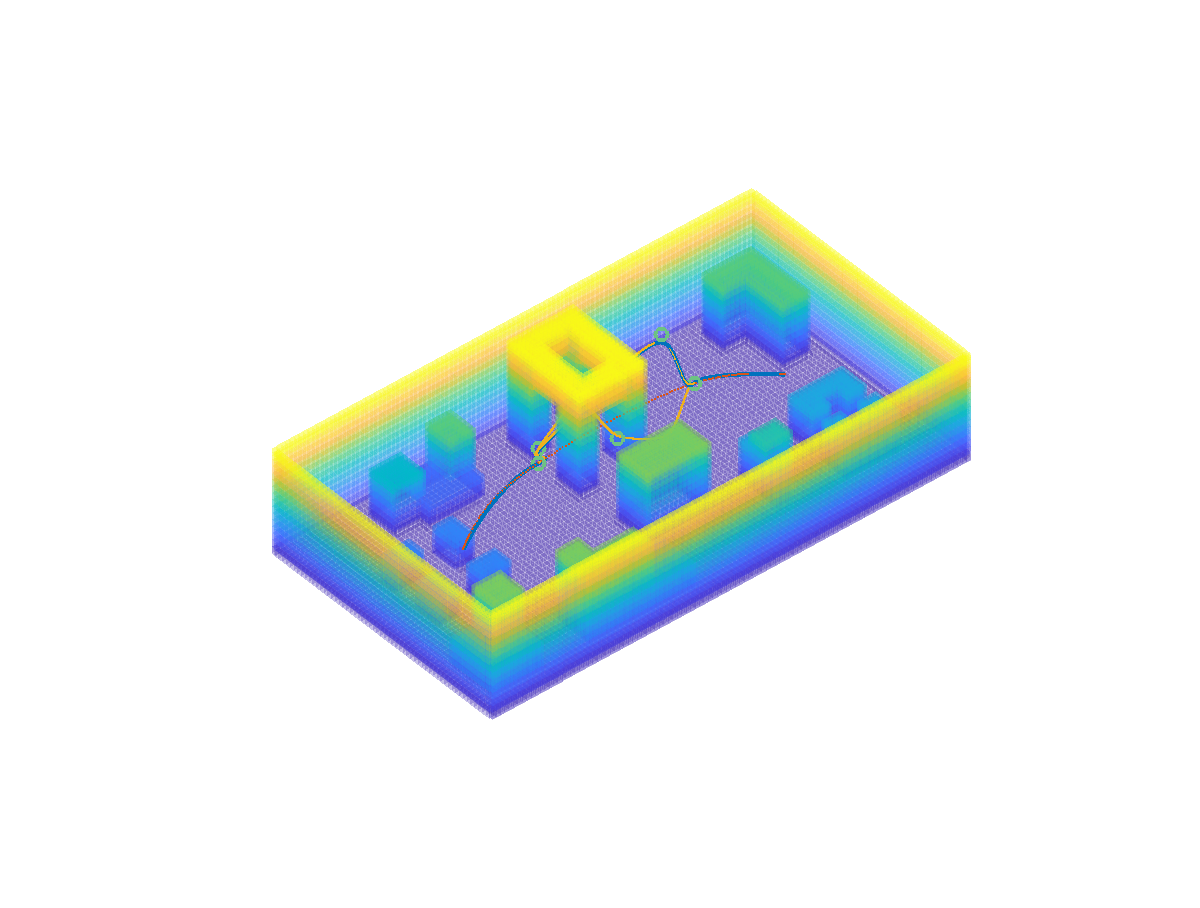
\includegraphics[trim={3.5cm 2.5cm 3cm 2.5cm}, clip = true, width = 1.05\textwidth]{Figs/Chapter6/replan_3d_traj_1.eps}}
		\end{minipage}
		\begin{minipage}{.45\linewidth}
			\centering
			\subfloat[]{%
				\label{FIG:REPLANNING-RESULTS-TRAJECTORY-B}%
				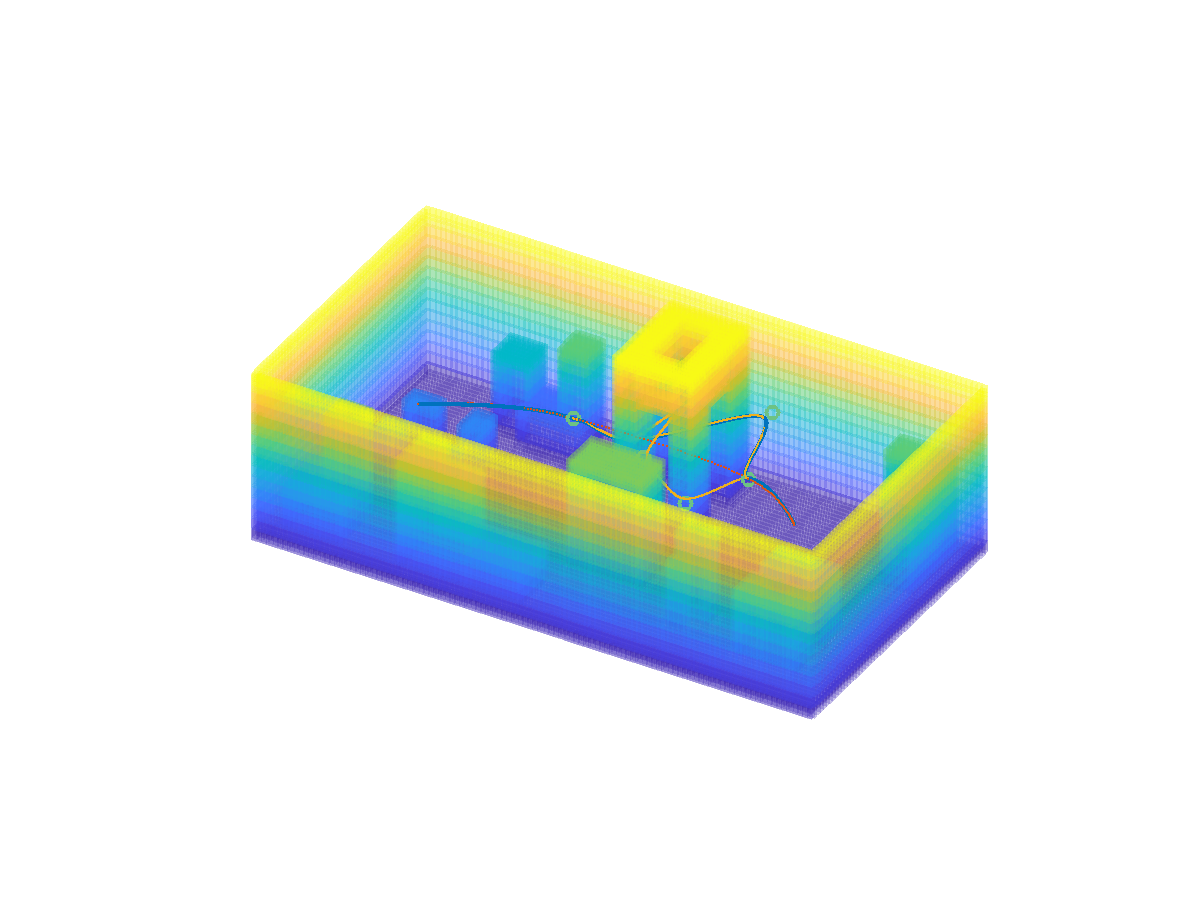
\includegraphics[trim={3.5cm 2.5cm 3cm 2.5cm}, clip = true, width = 1.05\textwidth]{Figs/Chapter6/replan_3d_traj.eps}}
		\end{minipage}
	\end{center}
	\caption{Results of the reviewed approach in the synthetic environment adopted in the Leonardo drone contest.
    The solution was able to replan feasible and safe trajectories in real-time, without forcing the quadcopter to an emergency stop.
    In the figure, the red path represents the initial colliding trajectory, the yellow points are the optimised hypothesis for replanned
    trajectory, and the blue path represents the final choice. Images (a) and (b) depict the same simulation, captured from two different
    points of view.}%
    \label{FIG:REPLANNING-RESULTS-TRAJECTORY}
\end{figure}
%%%%%%%%%%
The optimisation problem~\eqref{EQ:REPLANNING-SECOND-PHASE} yields to locally optimal trajectories guaranteed to be continuous up to
the second derivative, with the initial colliding trajectory. This is a fundamental feature since the tree segments, namely the first initial
trajectory, the replanned piece, and the final one, must be executed one after each other, consecutively.
Some issues may arise when the replanning procedure is called several times, during the execution of a previously replanned segment.
Indeed, the replanner may commission an even large number of trajectory pieces, that quickly become intractable for the reference generator.
Moreover, if the application at hand requires a higher level of continuity, this new requirement must be encoded inside~\eqref{EQ:REPLANNING-SECOND-PHASE}
which at the end may take too much time to solve.
In this section we propose a novel method to join the new replanned segment with a previously computed B-spline trajectory.
The proposed method is as simple as effective, it ensures continuity up to the spline order and outputs only one trajectory,
allowing for any replanning procedure as required by the surrounding environment.
The key idea comes from the B-spline property to be shaped, at each time instant $\splinevar \in \lps 0, T \rps$, by only $\order+1$
control points. It follows that, splitting the control points vector exactly in the correspondence of the final $(\order+1)$th control point
that spans the curve at time $t_{\text{start}}$ and the first control point that spans the curve at $t_{\text{goal}}$, allows for
inserting the new set of points, identifing the replanned curve, without loosing any spline continuity feature.
Finding the splitting points can be easily done by checking the knot span for the first $u_i \ge t_{\text{start}}$ and 
$u_j \ge t_{\text{goal}}$, then converting the found value in terms of the corresponding control point indeces $i_{\text{cp}}$
and $j_{\text{cp}}$ as
\begin{equation*}
    \begin{split}
        i_{\text{cp}} & = i - \left \lceil \order/2 \right \rceil - 2, \\
        j_{\text{cp}} & = j - \left \lceil \order/2 \right \rceil - 1. \\
    \end{split}
\end{equation*}
Giving two control points sequences $\CP^1 = \lps \bs{\cpoint}^1_0, \dots, \bs{\cpoint}^1_{\cpnumber^1} \rps$ and
$\CP^2 = \lps \bs{\cpoint}^2_0, \dots, \bs{\cpoint}^2_{\cpnumber^2} \rps$, with the corresponding knot vectors
$\bs{\splinevar}^1 = \Big[ 0_{0:\order}, \Delta^1_{\splinevar}, \dots,$ $(\cpnumber^1-\order)\Delta^1_{\splinevar}, T^1_{0:\order} \Big]$
and $\bs{\splinevar}^2 = \lps 0_{0:\order}, \Delta^2_{\splinevar}, \dots, (\cpnumber^2-\order)\Delta^2_{\splinevar}, T^2_{0:\order} \rps$,
representing the initial and replanned trajectory respectively, then the composed curve with control points
\begin{equation*}
    \CP = \lps \bs{\cpoint}^1_0, \dots, \bs{\cpoint}^1_{i_{\text{cp}}}, \bs{\cpoint}^2_0, \dots, \bs{\cpoint}^2_{\cpnumber^2}, \bs{\cpoint}^1_{j_{\text{cp}}}, \dots, \bs{\cpoint}^1_{\cpnumber^1} \rps,
\end{equation*}
and knot vector
\begin{equation*}
    \bs{\splinevar} =
    \begin{bmatrix}
        0_{0:\order}, & \Delta^1_{\splinevar}, & 2\Delta^1_{\splinevar}, & \dots, & ((\cpnumber^2 + \cpnumber^1 - j_{\text{cp}} + i_{\text{cp}}) - \order)\Delta^1_{\splinevar}, & T_{0:\order}
    \end{bmatrix},
\end{equation*}
preserves the path described by the consecution of the aforementioned three segments, ensuring continuity up to the chosen spline order.

\subsection{Experimental Results}
%%%%%%%%%%
\begin{figure}[!t]
	\begin{center}
		\begin{minipage}{.45\linewidth}
			\centering
			\subfloat[]{%
				\label{FIG:REPLANNING-RESULTS-VELOCITY-A}%
				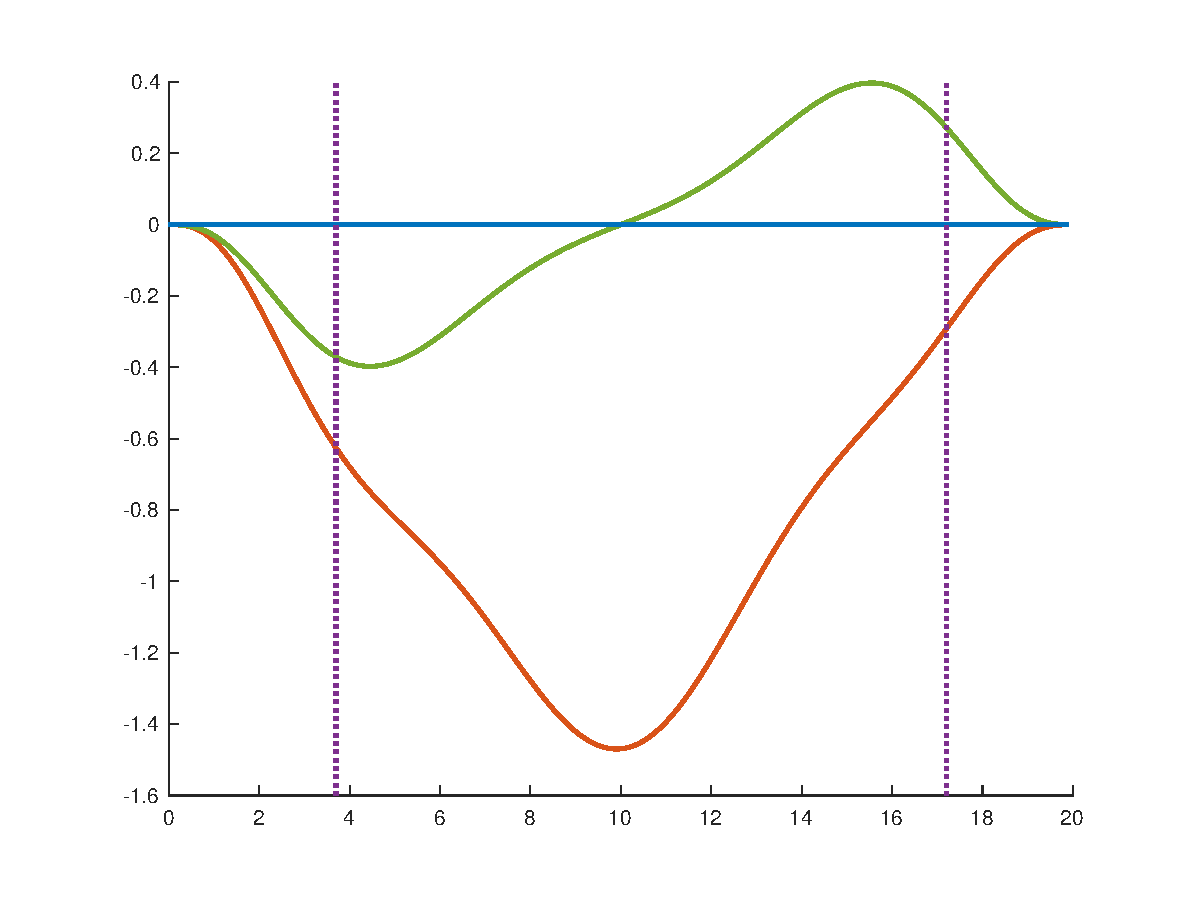
\includegraphics[width = 1.05\textwidth]{Figs/Chapter6/replan_init_vel.eps}}
		\end{minipage}
		\begin{minipage}{.45\linewidth}
			\centering
			\subfloat[]{%
				\label{FIG:REPLANNING-RESULTS-VELOCITY-B}%
				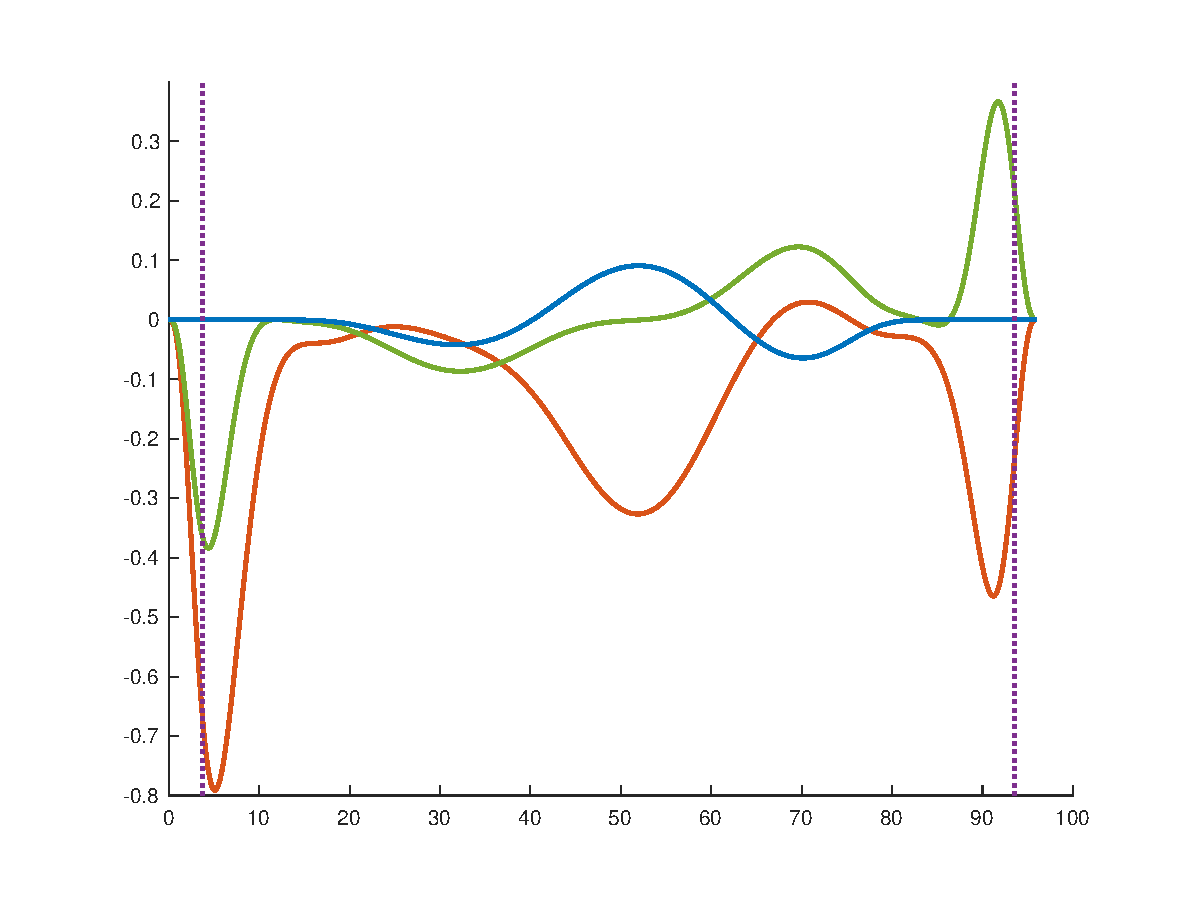
\includegraphics[width = 1.05\textwidth]{Figs/Chapter6/replan_post_vel.eps}}
		\end{minipage}
	\end{center}
	\caption{Initial velocity trajectory (a) and replanned one (b).
    In the images, the red line represents the velocity along the x-axis, the green one is the velocity along the y-axis,
    and the blue represents the velocity along the z-axis. The two vertical purple lines mark the initial and final cutting
    points, where the initial trajectory is broken and reconnected with the replanned one. Note that the velocity continuity
    is completely preserved. In both cases the velocity is kept below the safe level of $1.5m/s$.}%
    \label{FIG:REPLANNING-RESULTS-VELOCITY}
\end{figure}
%%%%%%%%%%
%%%%%%%%%%
\begin{figure}[!t]
	\begin{center}
		\begin{minipage}{.45\linewidth}
			\centering
			\subfloat[]{%
				\label{FIG:REPLANNING-RESULTS-ACCELERATION-A}%
				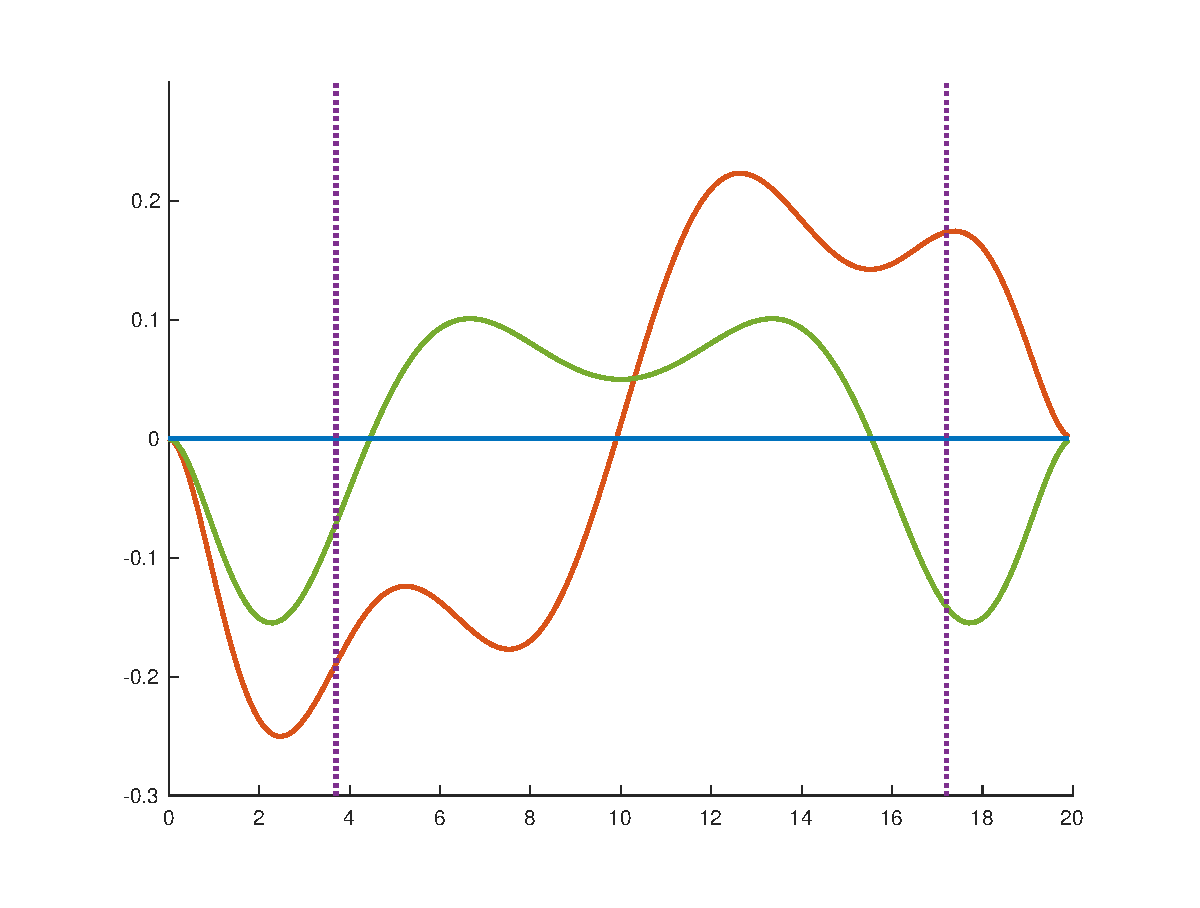
\includegraphics[width = 1.05\textwidth]{Figs/Chapter6/replan_init_acc.eps}}
		\end{minipage}
		\begin{minipage}{.45\linewidth}
			\centering
			\subfloat[]{%
				\label{FIG:REPLANNING-RESULTS-ACCELERATION-B}%
				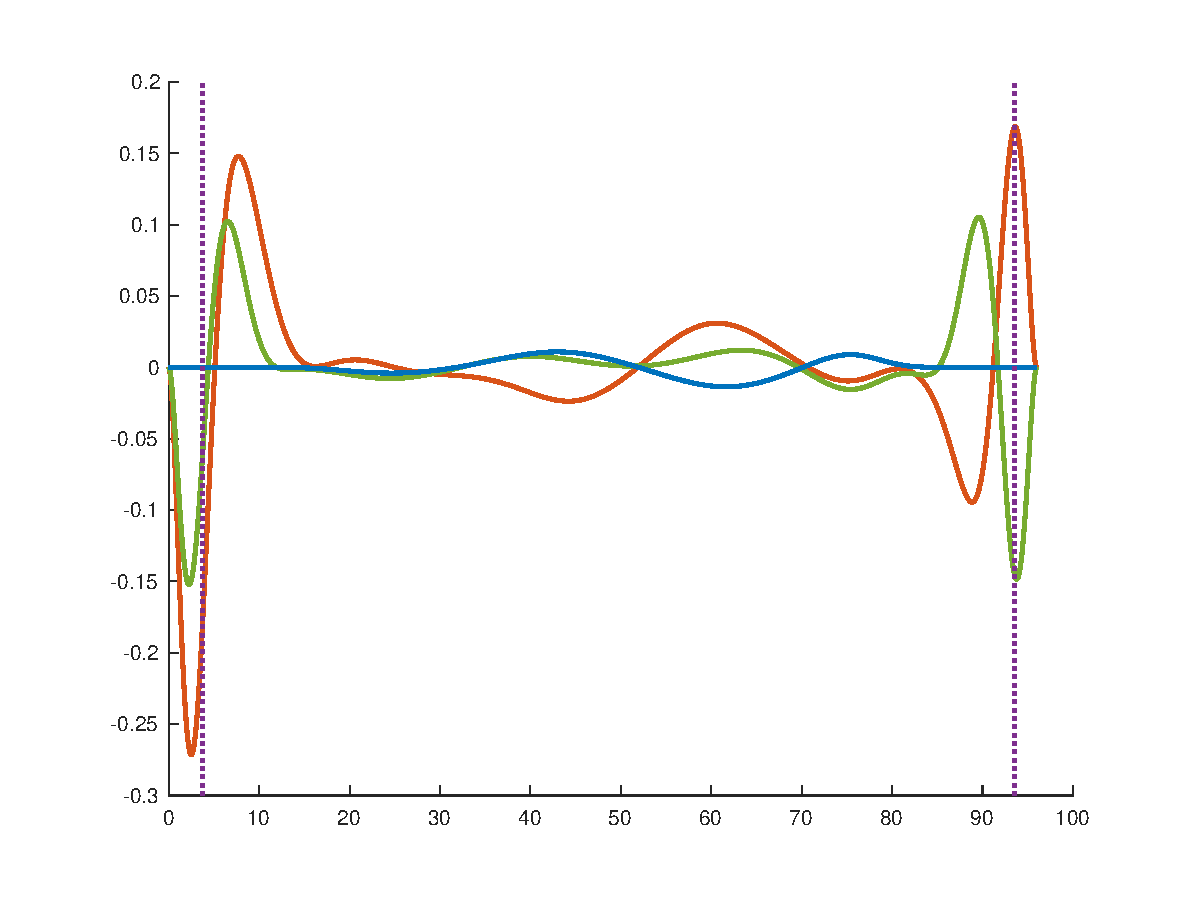
\includegraphics[width = 1.05\textwidth]{Figs/Chapter6/replan_post_acc.eps}}
		\end{minipage}
	\end{center}
	\caption{Initial acceleration trajectory (a) and replanned one (b).
    In the images, the red line represents the acceleration along the x-axis, the green one is the acceleration along the y-axis,
    and the blue represents the acceleration along the z-axis. The two vertical purple lines mark the initial and final cutting
    points, where the initial trajectory is broken and reconnected with the replanned one. Note that the acceleration continuity
    is completely preserved. In both cases the acceleration is kept below the safe level of $0.5m/s$.}%
    \label{FIG:REPLANNING-RESULTS-ACCELERATION}
\end{figure}
%%%%%%%%%%
%%%%%%%%%%
\begin{figure}[!t]
	\begin{center}
		\begin{minipage}{.45\linewidth}
			\centering
			\subfloat[]{%
				\label{FIG:REPLANNING-RESULTS-JERK-A}%
				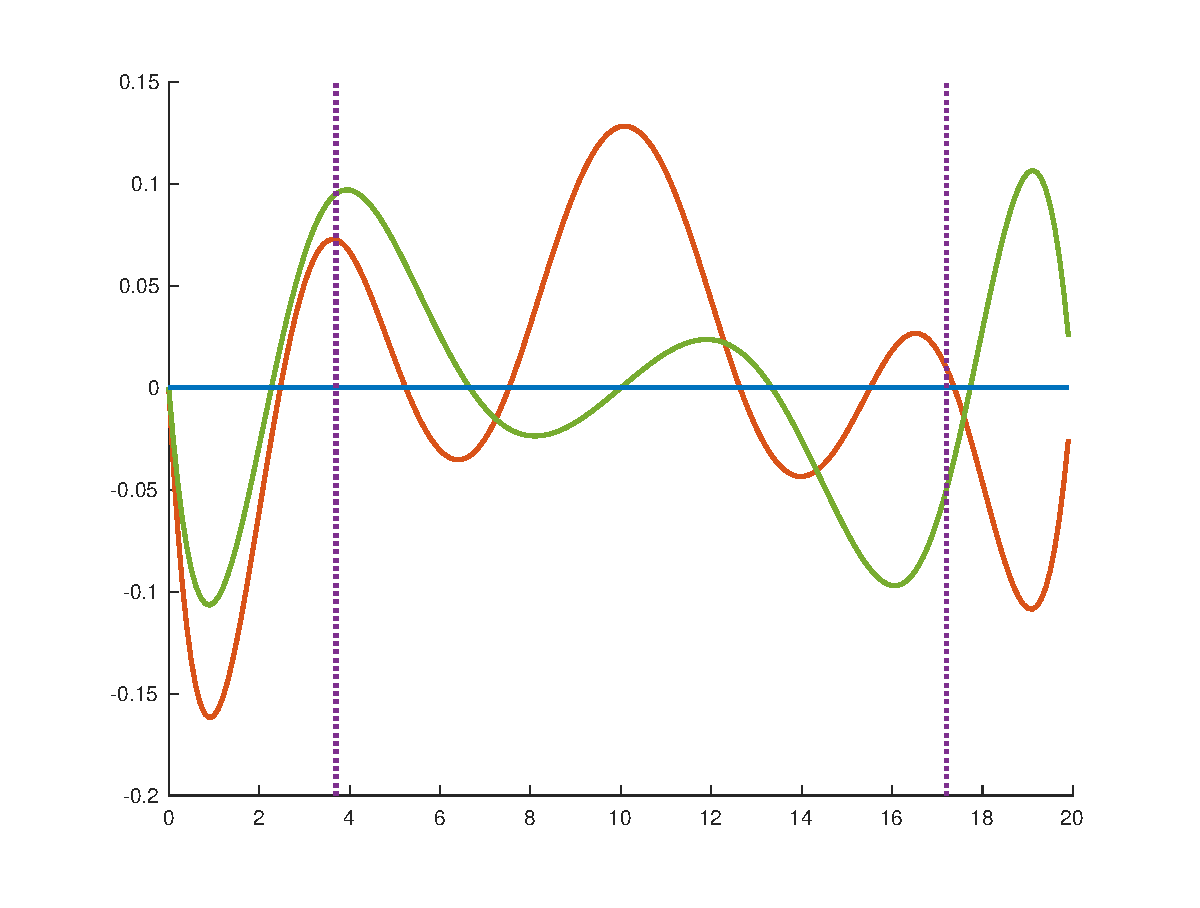
\includegraphics[width = 1.05\textwidth]{Figs/Chapter6/replan_init_jerk.eps}}
		\end{minipage}
		\begin{minipage}{.45\linewidth}
			\centering
			\subfloat[]{%
				\label{FIG:REPLANNING-RESULTS-JERK-B}%
				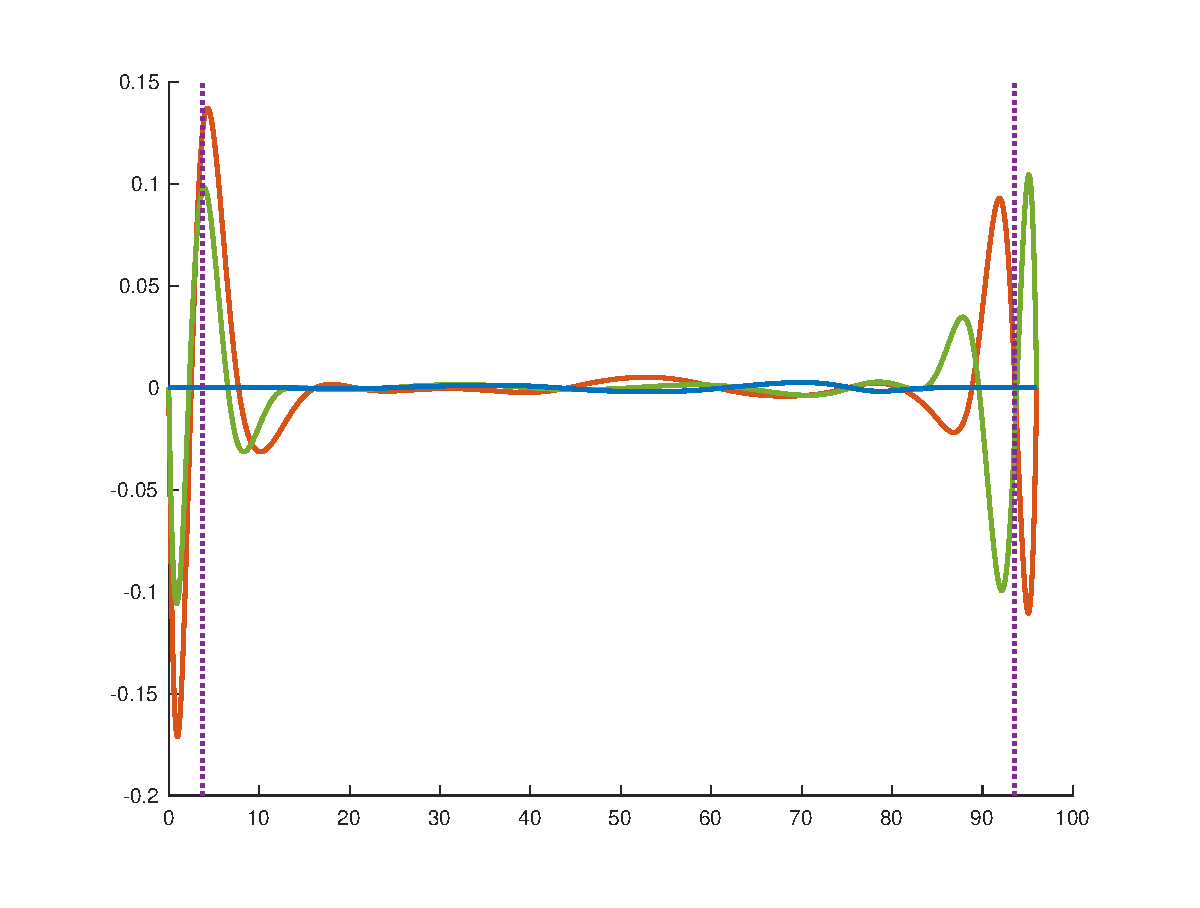
\includegraphics[width = 1.05\textwidth]{Figs/Chapter6/replan_post_jerk.eps}}
		\end{minipage}
	\end{center}
	\caption{Initial jerk trajectory (a) and replanned one (b).
    In the images, the red line represents the jerk along the x-axis, the green one is the jerk along the y-axis,
    and the blue represents the jerk along the z-axis. The two vertical purple lines mark the initial and final cutting
    points, where the initial trajectory is broken and reconnected with the replanned one. Note that the jerk continuity
    is completely preserved. No jerk limits have been fixed in this simulation.}%
    \label{FIG:REPLANNING-RESULTS-JERK}
\end{figure}
%%%%%%%%%%
%%%%%%%%%%
\begin{figure}[!t]
	\begin{center}
		\begin{minipage}{.45\linewidth}
			\centering
			\subfloat[]{%
				\label{FIG:REPLANNING-RESULTS-EXPLORATION-A}%
				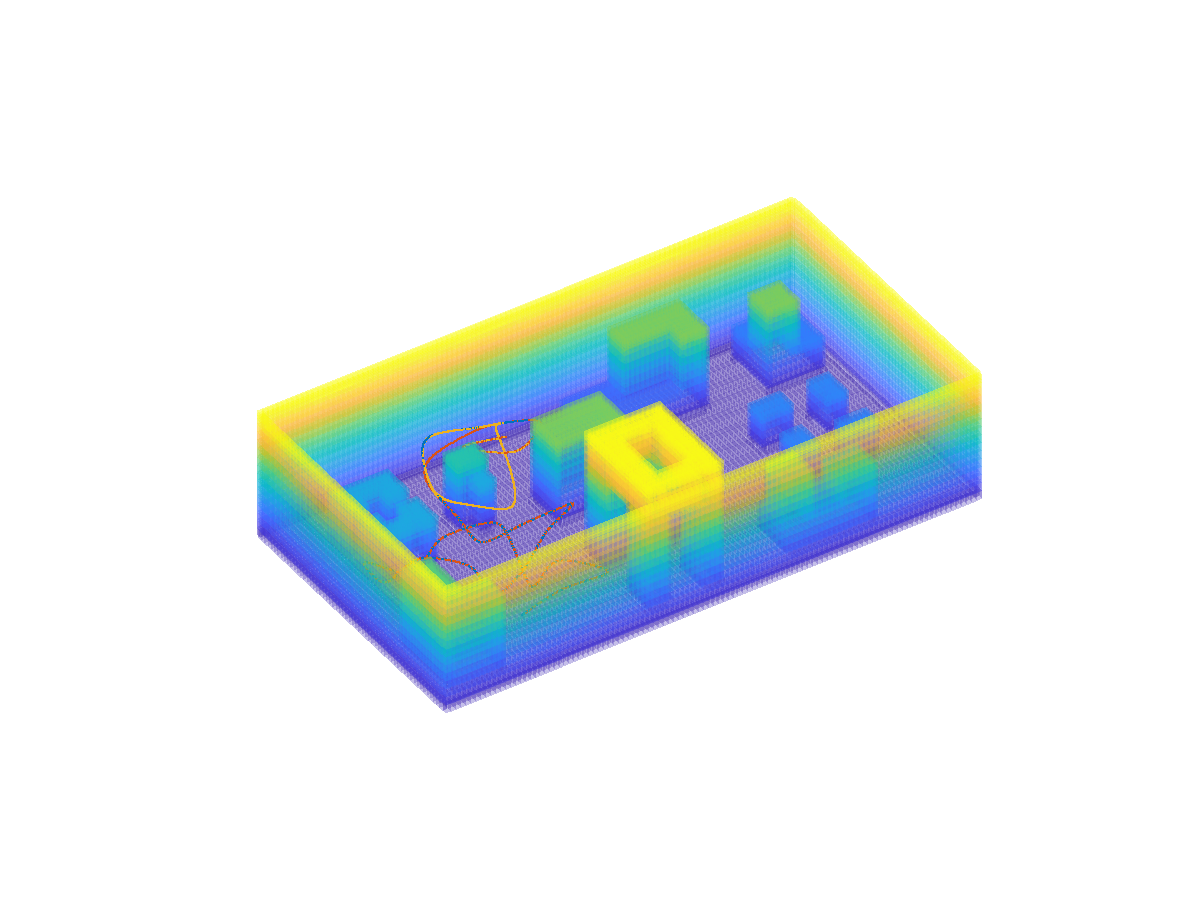
\includegraphics[trim={3.5cm 2.5cm 3cm 2.5cm}, clip = true, width = 1.05\textwidth]{Figs/Chapter6/replan_3d_traj_exploration_1.eps}}
		\end{minipage}
		\begin{minipage}{.45\linewidth}
			\centering
			\subfloat[]{%
				\label{FIG:REPLANNING-RESULTS-EXPLORATION-B}%
				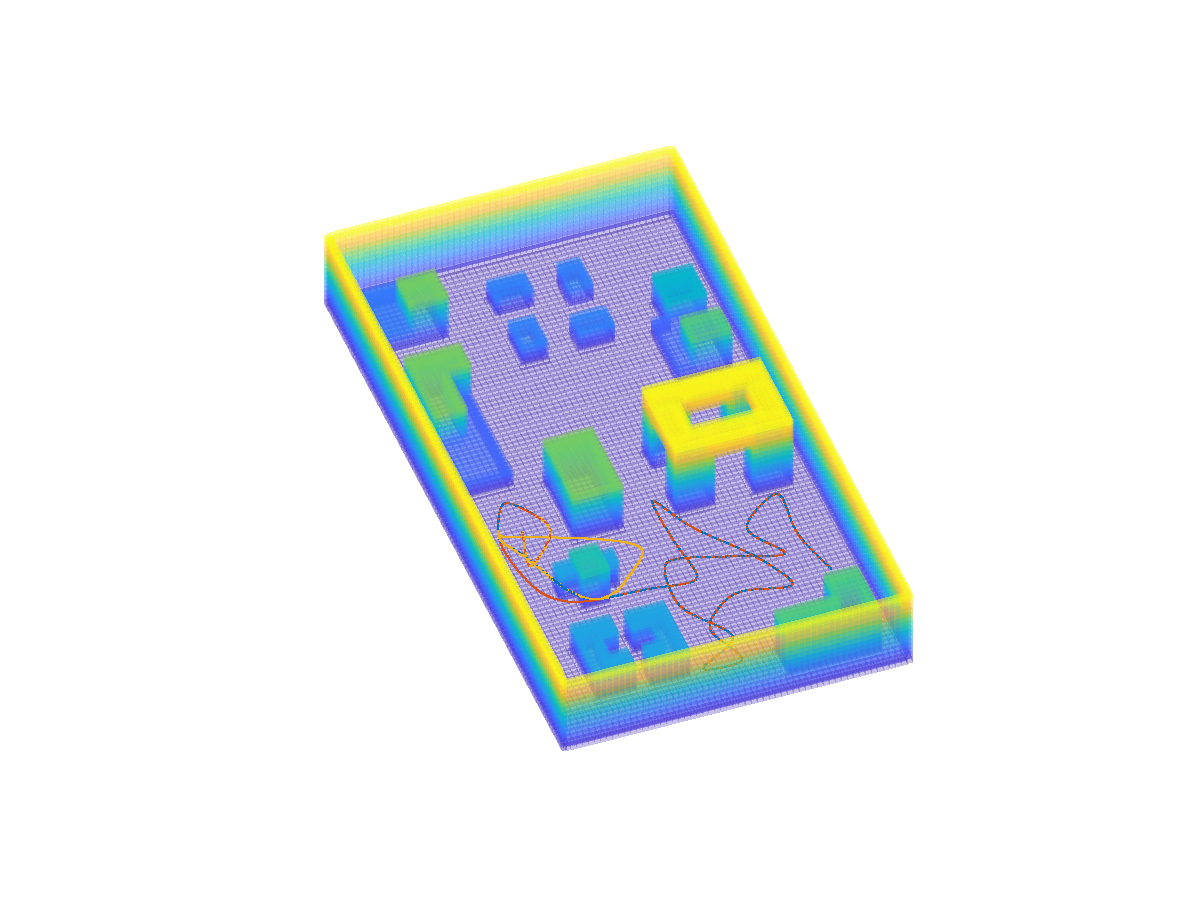
\includegraphics[trim={3.5cm 2.2cm 3cm 2.2cm}, clip = true, width = 1.05\textwidth]{Figs/Chapter6/replan_3d_traj_exploration.eps}}
		\end{minipage}
	\end{center}
	\caption{The reviewed approach applied to the specific case of exploration. In the image the trajectory has been replanned without a real
    collision in order to test its performance against previously unseen static obstacles, which may appear during the exploration task.
    As emerges from the figure, the replanning stack was able to successfully replan the exploring trajectory.}%
    \label{FIG:REPLANNING-RESULTS-EXPLORATION}
\end{figure}
%%%%%%%%%%
The proposed approach has been successfully applied to the synthetic environment proposed during the Leonardo drone challenge (see~\secref{SEC:DRONE-CONTEST}),
in two meaningful contexts. In the first stage, we supposed that the robot was performing a point-to-point trajectory to reach a particular area,
the committed initial trajectory was computed without the obstacles knowledge, leading to an unsafe motion. Next, we recreated the same 
exploration settings of~\secref{SEC:EXPLORATION-PROBLEM-DEFINITION}, where the robot was performing an exploration task driven by the
algorithm proposed in~\secref{SEC:SEARCH-PATROLLING-PERSPECTIVE}. In this second case, the initial trajectory was computed using the
environment knowledge, thus the performed trajectory was not in collision with obstacles, in order to trigger the replanning procedure
we inject a false sensor update containing an obstacle exactly on the motion direction.
The obtained results are reported in~\figref{FIG:REPLANNING-RESULTS-TRAJECTORY} for the first case, and in~\figref{FIG:REPLANNING-RESULTS-EXPLORATION}
for the exploration case. In both the images is reported the environment occupancy map, the initial trajectories, the optimised ones, and the sampled nodes.
In particular, the red continuous line represents the initial colliding motion, which requires replanning, in~\figref{FIG:REPLANNING-RESULTS-TRAJECTORY}
the collision is particularly clear, while in~\figref{FIG:REPLANNING-RESULTS-EXPLORATION} the red path is not colliding with any obstacles due to the
false measurement injected. The green circles represent the topologically different sampled and then shortened paths, the yellow lines are the 
trajectories obtained after path-guided optimisation, and the blue line is the final selected trajectory.
As the reader can notice, the blu line is always overlapped to the red one in the beginning end at the end, while is overlapped to the
yellow one inside the replanned segment. Figures~\ref{FIG:REPLANNING-RESULTS-VELOCITY},~\ref{FIG:REPLANNING-RESULTS-ACCELERATION},
and~\ref{FIG:REPLANNING-RESULTS-JERK} show the behavior of velocity, acceleration, and jerk before and after replanning.
In the images, the red lines are the quantities along the x-axis, the green ones are the same quantities along the y-axis, and the
z-axis is shown in blue. The purple vertical lines remark the start and goal points, where the initial colliding trajectory has been broken.
Note how the continuity is preserved, among the different trajectory segments, up to the chosen trajectory order $\order$.
A full list of parameters used to carry out the aforementioned simulations is reported in~\tabref{TAB:REPLANNING-PARAMETERS}.
%%%%%%%%%
{
\renewcommand{\arraystretch}{1.35}
\begin{table}[b!]
    \centering
    \begin{tabular}{||c|c||c|c||}
        \hline
        \hline
        $v_{\text{max}}$ & $1.5m/s$ & $a_{\text{max}}$ & $0.5m/s^2$ \\
        \hline
        $T_{\text{max}}$ & $2.0s$ & $\Delta_T$ & $0.1s^2$ \\
        \hline
        $T_{\text{min}}$ & $0.5s$ & $N_{\text{min}}$ & $3$ \\
        \hline
        $d_{\text{obs}}$ & $4m$ & $\Delta_{\text{max}}$ & $0.1s$ \\
        \hline
        $N_{\text{max}}$ & $3000$ & $d_{\text{res}}$ & $0.2m$ \\
        \hline
        $d_{\text{safe}}$ & $0.5m$ & $p$ & $7$ \\
        \hline
        $\lambda_1$ & $1.0$ & $\lambda_2$ & $10.0$ \\
        \hline
        \hline
    \end{tabular}
    \caption{Parameters used to test the replanning algorithm.}%
	\label{TAB:REPLANNING-PARAMETERS}
\end{table}}
%%%%%%%%%

%----------------------------------------------------------------------------------------
\section{Spatio-Temporal Curves Separation}%
\label{SEC:SPATION-TEMPORAL-SEPARATION} 
Despite the effectiveness of the replanning algorithm described in~\secref{SEC:REPLANNING-ALGORITHM}, it may fail in environments where
are present moving objects, as these are all treated as static obstacles. This simplifying assumption can be fatal to the replanning procedure
as the final trajectory may still be unsafe during the next time instant.
In this view, we proposed a novel approach to the replanning problem described in~\secref{SEC:REPLANNING-PROBLEM-DEFINITION}, in the
setting where the safe set is not fixed in time, thus moving obstacles may cross the robot motion.
The proposed solution is grounded on the assumption to have a priori knowledge of the surrounding environment, as well as an estimation
of the obstacle to which the agent may collides. We stress the fact that, even if we especially focus on the particular case of one single
moving obstacle, the proposed approach can easily extended to the multi-objects or multi-agent ones, where some of them are static.

Motivated by the success of GTO approaches~\cite{zhou2020robust, oleynikova2016continuous, gao2017gradient, usenko2017real}, and inspired by
the flexibility of B\acuteacc ezier curves in trajectory planning~\cite{gao2019flying, mehdi2015collision, park2020efficient}, we propose
a novel optimisation-based replanning paradigm where the B\acuteacc ezier parameterisation is employed twice in expressing the path and the associated timing law.
The final trajectory recalls the same structure chosen in~\secref{SEC:EXPLORATION-TRAJECTORY-PARAMETERISATION}, where the piecewise
structure allows for splitting the planning problem in several segments, and considering one environment area, or obstacle collision, at a time.
In the next sections we firstly remark how the double parameterisation is the key to fast plan optimal avoiding trajectories and state 
the final trajectory equations (\secref{SEC:ST-PARAM-COMPOSITION}), then we formulate the proposed solution as a single step optimisation
problem (\secref{SEC:ST-SEPARATION}).

\subsection{Spatio-Temporal Parameterisation \& Composition}%
\label{SEC:ST-PARAM-COMPOSITION}
%%%%%%%%%%
\begin{figure}[!t]
	\centering
	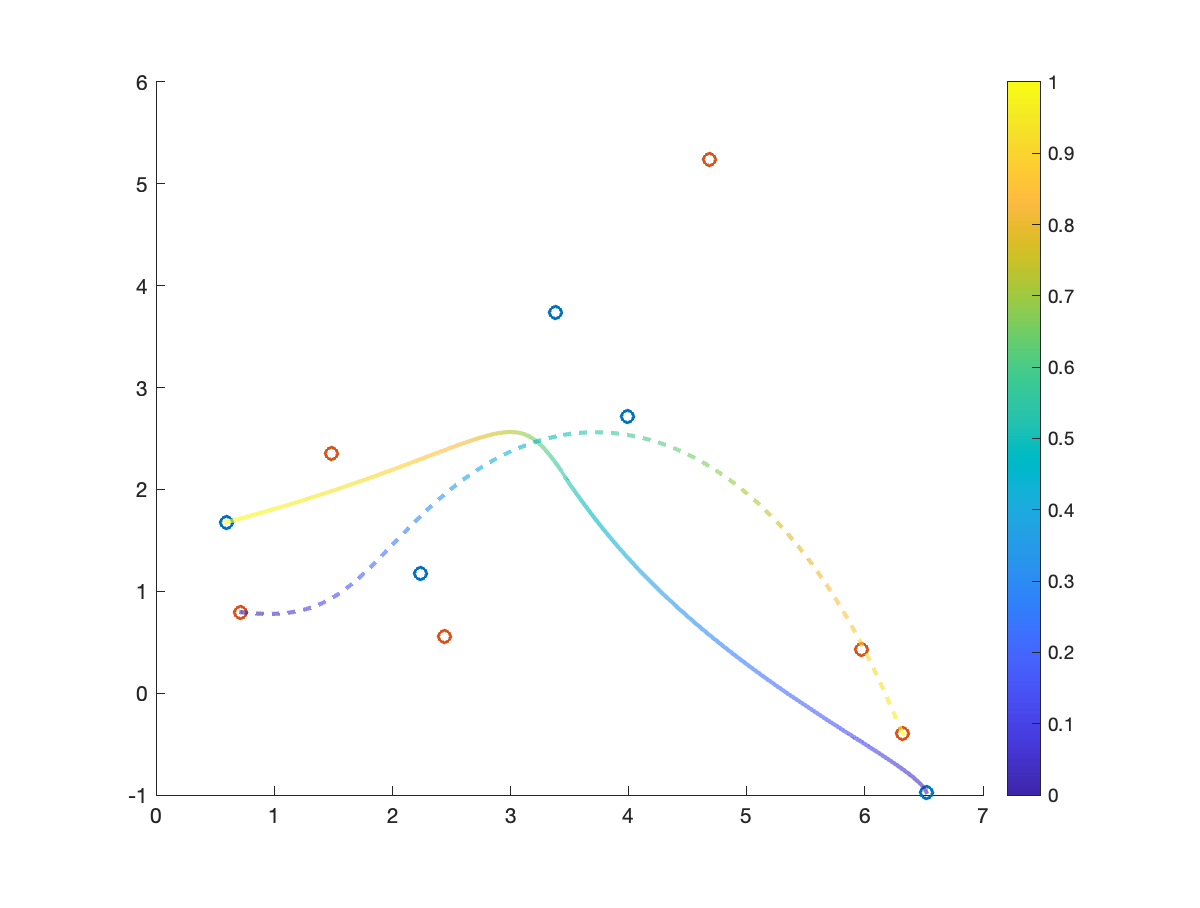
\includegraphics[width=0.6\textwidth]{Figs/Chapter6/st_bezier_timetraj_coll.eps}
	\caption{Example of two colliding B\acuteacc ezier curves. In the figure, the blue circles represent the randomly sampled
    control points of the continuous curve, while the red ones are the randomly sampled control points of the dotted one.
    The two curves are obtained as the composition of two B\acuteacc ezier curves of order $5$ for the position and $3$ for
    the timing law. The color shadows represent the time behavior of the two curves, normalized inside the interval $\lps 0, 1\rps$.}
	\label{FIG:ST-BEZIER-COLLIDING-TRAJ}
\end{figure}
%%%%%%%%%%
%%%%%%%%%%
\begin{figure}[!t]
	\centering
	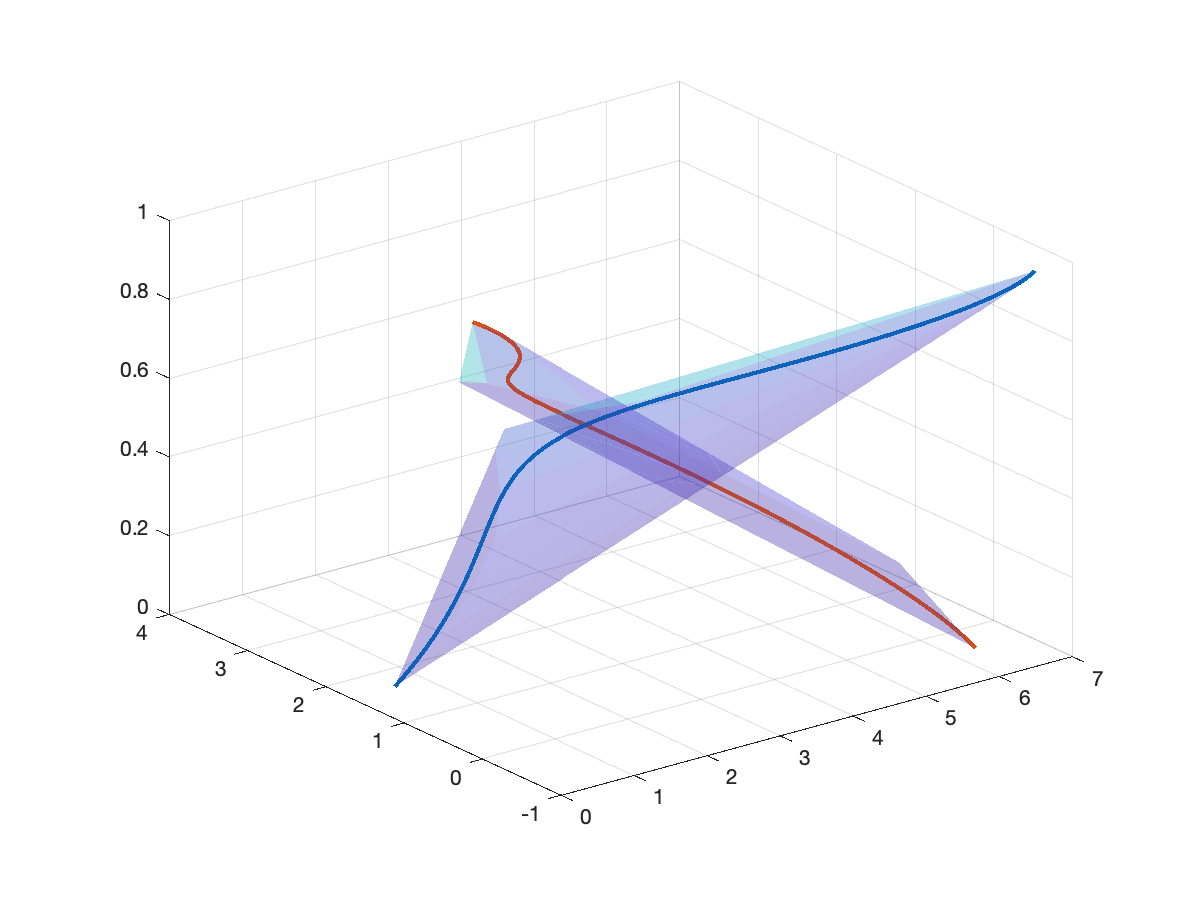
\includegraphics[width=0.6\textwidth]{Figs/Chapter6/st_bezier_convexhull_coll.eps}
	\caption{Convex hull representation of~\figref{FIG:ST-BEZIER-COLLIDING-TRAJ}. The third dimension is represented by the time,
    normalized inside the interval $\lps 0, 1\rps$.}
	\label{FIG:ST-BEZIER-COLLIDING-CONVEX}
\end{figure}
%%%%%%%%%%
The key idea behind the proposed solution is to parametrise both path and timing law by means of two B\acuteacc ezier curves.
In order to understand how this choice may helps during the planning stage, let us consider the example reported in~\figref{FIG:ST-BEZIER-COLLIDING-TRAJ}.
In this 2-dimensional case, two $5$-order B\acuteacc ezier curves
\begin{equation*}
    \begin{split}
        \rr & = \sum_{i = 0}^{\order} \bs{\cpoint}_i \basis_i^{\order} \lp \splinevar \rp, \\
        \rr^{o} & = \sum_{i = 0}^{\order} \bs{\cpoint}_i^{o} \basis_i^{\order} \lp \splinevar^{o} \rp,
    \end{split}
\end{equation*}
with $\order = 5$ and $\bs{\cpoint}_i$, $\bs{\cpoint}_i^{o}$ randomly sampled in $\R^2$.
The timing laws fixing $\splinevar$ and $\splinevar^{o}$ are chosen as other two B\acuteacc ezier curves ensuring the contidition
$\splinevar \in \lps 0, 1 \rps$ for any $t \in \R_{\ge 0}$
\begin{equation*}
    \begin{split}
        \splinevar & = \sum_{i = 0}^{\order_{\splinevar}} \splinevar_i \basis_i^{\order_{\splinevar}} \lp t \rp, \\
        \splinevar^{o} & = \sum_{i = 0}^{\order_{\splinevar}} \splinevar_i^{o} \basis_i^{\order_{\splinevar}} \lp t \rp.
    \end{split}
\end{equation*}
In the aforementioned relation, $\order_{\splinevar} = 3$, while $\splinevar_0 = \splinevar_0^o = 0$ and 
$\splinevar_{\order_{\splinevar}} = \splinevar_{\order_{\splinevar}}^o = 1$ to constraining $\splinevar, \splinevar^o \in \lps 0,1 \rps$.
The remaining free points have been selected randomly in $\R$.
In this settings, $\rr$ is thought of as the robot trajectory, while $\rr^{o}$ as the obstacle one.~\figref{FIG:ST-BEZIER-COLLIDING-TRAJ}
depicts the curves behavior on the $\R^2$ plane and along time thanks the reported colormap, in particular $\rr$ is depicted as a continuous line,
with the blue circles as associated control points, while $\rr^o$ is represented as a dotted line, with the orange circles as control points.
The reader can immediately recognize a possible collision around $0.5/0.6$ seconds, where the two lines cross each other.
The replanning problem may be solved just by moving the path control points $\bs{\cpoint}_i$, leading to a very huge detour from the initial
planned trajectory, or by slowing down the agent until its motion is safe from possible collisions.
In this second case, instead of moving the position control points we require to change the timing law, making the agent trajectory slower
and with a higher execution time. Although very appealing, the latter solution is not feasible as long as the relation between
the timing law and the induced agent-obstacle distance is not clear.
In this framework, the B\acuteacc ezier curve properties help us in formalizing such a relation exploiting first the composition rule,
then the difference rule, and finally the product one. Although the reader can find a complete analysis in~\secref{SEC:SPLINES-APPENDIX},
we recall here these properties applied to the considered specific case.
Let us suppose we want formalize the agent-obstacle squared distance $d \lp t \rp$ as a B\acuteacc ezier curve, whose control points $d_i$ must
be function of the initial quantities $\bs{\cpoint}_i$, $\bs{\cpoint}_i^o$, $\splinevar_i$, and $\splinevar_i^o$.
Applying the composition rule to $\rr$ and $\splinevar$, and $\rr^o$ and $\splinevar^o$ leads to
\begin{equation}%
    \label{EQ:ST-BEZIER-COMPOSITION-A}
    \begin{split}
        \bs{\cpoint}_{\splinevar_i} & = \lambda_{0,j}^{\order} \hspace{0.3cm} j = 0, \dots, \order \order_{\splinevar}, \\
        \bs{\cpoint}_{\splinevar_i}^o & = \rho_{0,j}^{\order} \hspace{0.3cm} j = 0, \dots, \order \order_{\splinevar},
    \end{split}
\end{equation}
where
\begin{equation}%
    \label{EQ:ST-BEZIER-COMPOSITION-B}
    \begin{split}
        \lambda_{i,j}^k =
        \begin{pmatrix}
            k \order_{\splinevar} \\ j
        \end{pmatrix}^{-1}
        \sum_{l = \max \lp 0, j - \order_{\splinevar} \rp}^{\min \lp j, k \order_{\splinevar} - \order_{\splinevar} \rp} &
        \begin{pmatrix}
            k \order_{\splinevar} - \cpnumber_u \\ l
        \end{pmatrix}
        \begin{pmatrix}
            \order_{\splinevar} \\ j-l
        \end{pmatrix} \\
        & \lps \lp 1-\splinevar_{j-l} \rp \lambda_{i,l}^{k-1} + \splinevar_{j-l}\lambda_{i+1,l}^{k-1} \rps,
    \end{split}
\end{equation}
\begin{equation}%
    \label{EQ:ST-BEZIER-COMPOSITION-C}
    \begin{split}
        \rho_{i,j}^k =
        \begin{pmatrix}
            k \order_{\splinevar} \\ j
        \end{pmatrix}^{-1}
        \sum_{l = \max \lp 0, j - \order_{\splinevar} \rp}^{\min \lp j, k \order_{\splinevar} - \order_{\splinevar} \rp} &
        \begin{pmatrix}
            k \order_{\splinevar} - \cpnumber_u \\ l
        \end{pmatrix}
        \begin{pmatrix}
            \order_{\splinevar} \\ j-l
        \end{pmatrix} \\
        & \lps \lp 1-\splinevar^o_{j-l} \rp \rho_{i,l}^{k-1} + \splinevar^o_{j-l}\rho_{i+1,l}^{k-1} \rps,
    \end{split}
\end{equation}
for $k = 1, \dots, \order$, $i = 0, \dots, \order-k$, and $j = 0, \dots, k\order_{\splinevar}$ and setting
$\lambda_{i,0}^{0} = \bs{\cpoint}_i$. The obtained control points $\bs{\cpoint}_{\splinevar_i}$ and
$\bs{\cpoint}_{\splinevar_i}^o$ represent two new curves of order $\order \order_{\splinevar}$, encoding both
path and timing law, then the agent-obstacle distance, along the two axis, can be evaluated as
\begin{equation}%
    \label{EQ:ST-BEZIER-COMPOSITION-D}
    \bs{\cpoint}_{\Delta_i} = \bs{\cpoint}_{\splinevar_i} - \bs{\cpoint}_{\splinevar_i}^o \hspace{0.3cm} \forall i = 0, \dots, \order \order_{\splinevar}.
\end{equation}
The final step consists in converting the axis-wise distance, to a squared Euclidean one.
To do this, $\bs{\cpoint}_{\Delta_i} = \lps \bs{\cpoint}_{\Delta_i}^x, \bs{\cpoint}_{\Delta_i}^y\rps$
must be first decomposed alog the two axis, then each component must be squared up as
\begin{equation}%
    \label{EQ:ST-BEZIER-COMPOSITION-E}
    \lp \bs{\cpoint}_{\Delta_i}^k \rp^2 =
    \sum_{j = \max \lp 0, i-\order \order_{\splinevar}2 \rp}^{\min \lp \order \order_{\splinevar}, i \rp}
    \frac{
        \begin{pmatrix}
            \order \order_{\splinevar} \\ j
        \end{pmatrix}
        \begin{pmatrix}
            \order \order_{\splinevar} \\ i-j
        \end{pmatrix}
    }{
        \begin{pmatrix}
            2\order \order_{\splinevar} \\ i
        \end{pmatrix}
    }
    \bs{\cpoint}_{\Delta_j}^k \bs{\cpoint}_{\Delta_{i-j}}^k,
\end{equation}
with $k = x,y$ and $i = 0, \dots, 2\order \order_{\splinevar}$.
Finally, the squared Euclidean distance can be evaluated as a B\acuteacc ezier curve $d \lp t \rp$ of order $2\order \order_{\splinevar}$
with control points
\begin{equation}%
    \label{EQ:ST-BEZIER-COMPOSITION-F}
    d_i = \lp \bs{\cpoint}_{\Delta_i}^x \rp^2 + \lp \bs{\cpoint}_{\Delta_i}^y \rp^2.
\end{equation}
\begin{remark}
    Equations~\eqref{EQ:ST-BEZIER-COMPOSITION-A}-\eqref{EQ:ST-BEZIER-COMPOSITION-F} look complicated, but at the end, the relation
    between $d_i$ and $\bs{\cpoint}_i$, $\splinevar_i$, $\bs{\cpoint}_i^o$, and $\splinevar^o_i$ results to be a simple algebraic relation.
    Let define the map $\Gamma : \R^{2(\order+\order_{\splinevar})} \mapsto \R^{2 \order \order_{\splinevar}}$ as the function mapping the
    initial path and time control points to the final squared Euclidean distance.
\end{remark}
\begin{remark}
    Equations~\eqref{EQ:ST-BEZIER-COMPOSITION-A}-\eqref{EQ:ST-BEZIER-COMPOSITION-F} have been developed for a planar case,
    but the extension to the three-dimension case is straightforward, considering $\bs{\cpoint}, \bs{\cpoint}^o \in \R^3$ and
    $k = x,y,z$.
\end{remark}
The key idea behind the proposed approach lies in the possibility to separate the agent curve and the obstacle one both in space, and
time, letting the algorithm to select the optimal trade-off between moving the position control points, or the timing law ones.
The adopted B\acuteacc ezier parameterisation is crucial in this view since it allows to continuously keep separated the two curves, and
straightforwardly join them when is required. A graphical representation of this property is depicted in~\figref{FIG:ST-BEZIER-COLLIDING-CONVEX},
where is reported a convex hull representation of the colliding curves shown in~\figref{FIG:ST-BEZIER-COLLIDING-TRAJ}.
In~\figref{FIG:ST-BEZIER-COLLIDING-CONVEX} the two-dimensional curves are depicted in $\R^3$, with the time being the third axis.
This three-dimensional representation has been obtained enlarging the set of composed control points from~\eqqref{EQ:ST-BEZIER-COMPOSITION-A},
with $\splinevar_i$ and $\splinevar_i^o$. The resulting trajectories are still B\acuteacc ezier curves, thus the convex hull 
containment property still holds, and the obtained polyhedra can be used to verify collisions both in time and space.

We conclude this section by recalling the piecewise B\acuteacc ezier structure defined in~\secref{SEC:EXPLORATION-TRAJECTORY-PARAMETERISATION},
used here to represent the final quadcopter trajectory.
\begin{equation}%
    \label{EQ:ST-SEPARATION-PIECEWISE}
	\rr \lp t \rp=
	\begin{cases}
		\sum_{i=0}^{\order} \basis_i^{\order}(\splinevar_1 \lp \clock_1 \rp) \bs{\cpoint}^1_i & \hspace{-0.2cm} t \in [T_0, T_1],\\
		\sum_{i=0}^{\order} \basis_i^{\order}(\splinevar_2 \lp \clock_1 \rp) \bs{\cpoint}^2_i & \hspace{-0.2cm} t \in [T_1, T_2],\\
		\hspace{0.2cm} \vdots & \vdots \\
		\sum_{i=0}^{\order} \basis_i^{\order}(\splinevar_{\segnumber} \lp \clock_{\segnumber} \rp) \bs{\cpoint}^{\segnumber}_i & \hspace{-0.2cm} t \in [T_{\segnumber-1}, T_{\segnumber}],\\
	\end{cases}
\end{equation}
with $\clock_i = \frac{t-T_{i-1}}{T_{i}-T_{i-1}}$ and $\splinevar_j \lp \clock_j \rp = \sum_{i=0}^{\order_{\splinevar}} \basis_i^{\order_{\splinevar}}(\clock_j) \splinevar^j_i$.
From now on we suppose $\order = 5$ and $\order_{\splinevar} = 3$.

\subsection{Spatio-Temporal Separation}%
\label{SEC:ST-SEPARATION}
%%%%%%%%%%
\begin{figure}[!t]
	\begin{center}
		\begin{minipage}{.45\linewidth}
			\centering
			\subfloat[]{%
				\label{FIG:ST-BEZIER-2D-SETTING-A}%
				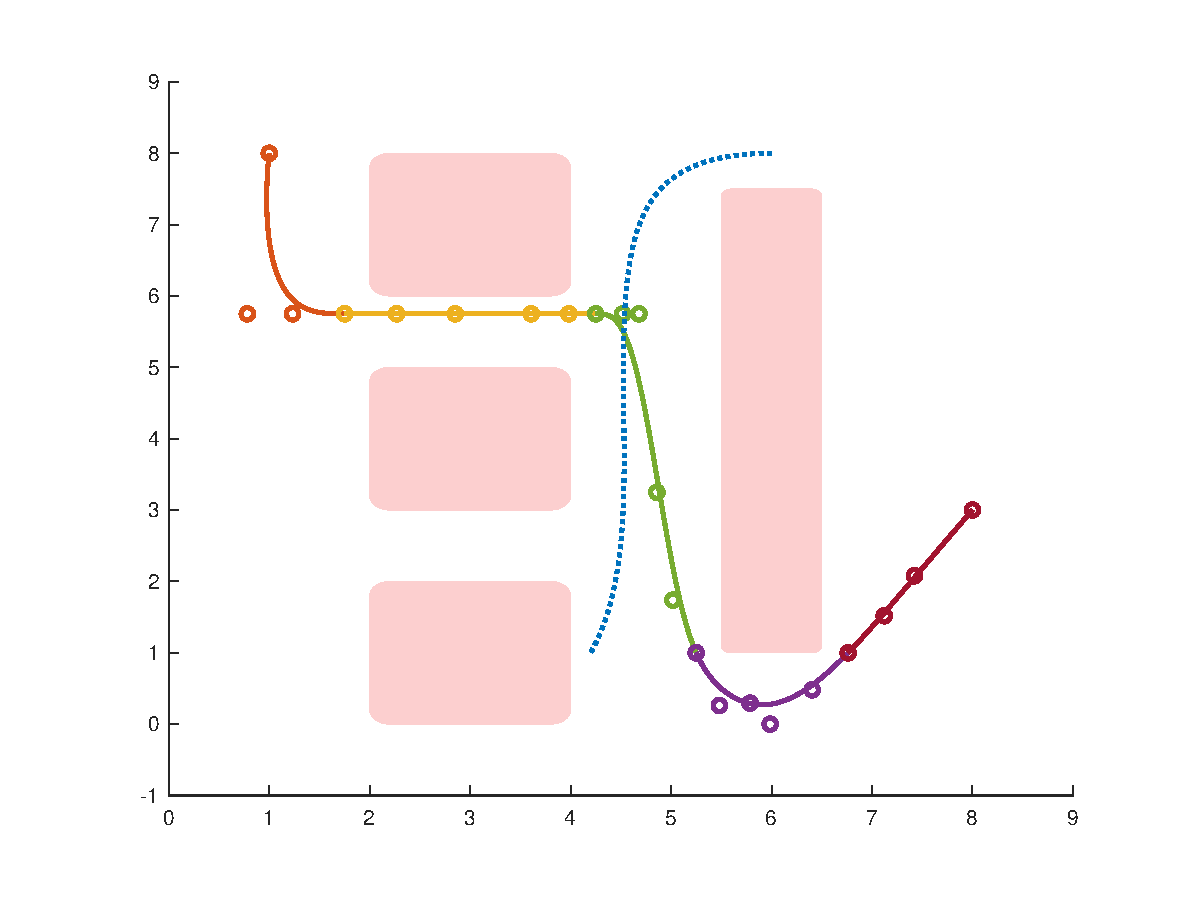
\includegraphics[width = 1.05\textwidth]{Figs/Chapter6/st_bezier_inital_setting_2d.eps}}
		\end{minipage}
		\begin{minipage}{.45\linewidth}
			\centering
			\subfloat[]{%
				\label{FIG:ST-BEZIER-2D-SETTING-B}%
				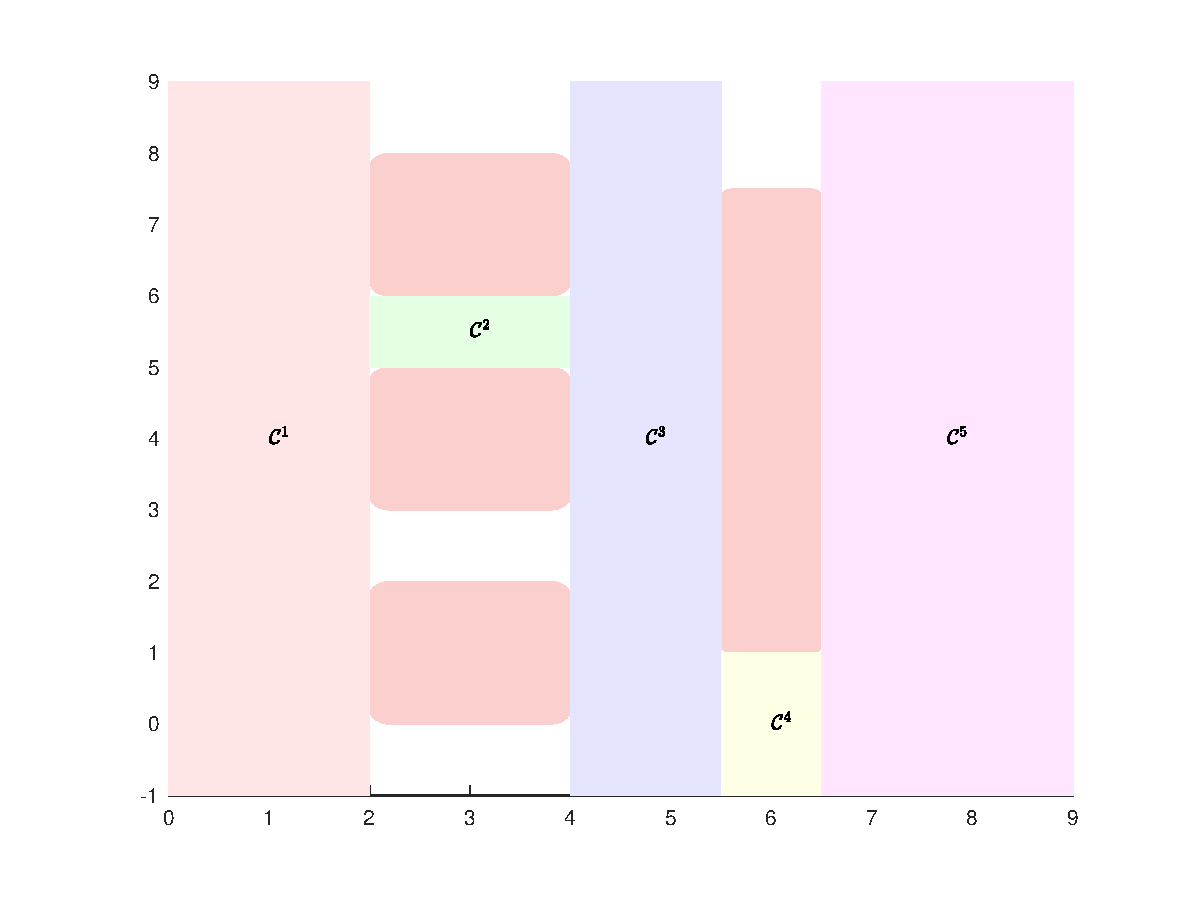
\includegraphics[width = 1.05\textwidth]{Figs/Chapter6/st_bezier_corridors_2d.eps}}
		\end{minipage}
	\end{center}
	\caption{Experimental setting used to test the proposed approach. Figure (a) depicts the initial trajectory planning made using the
    corridords depicted in image (b). The colored lines represent the initial agent trajectory, along with the respective selected control points,
    while the dotted blue line is the moving obstacle path, chosen in order to get in collision with the third green piece. The red 
    rectangles are environment obstacles assumed to be completely known.}%
    \label{FIG:ST-BEZIER-2D-SETTING}
\end{figure}
%%%%%%%%%%
%%%%%%%%%%
\begin{figure}[!t]
	\begin{center}
		\begin{minipage}{.45\linewidth}
			\centering
			\subfloat[]{%
				\label{FIG:ST-BEZIER-2D-INITIAL-A}%
				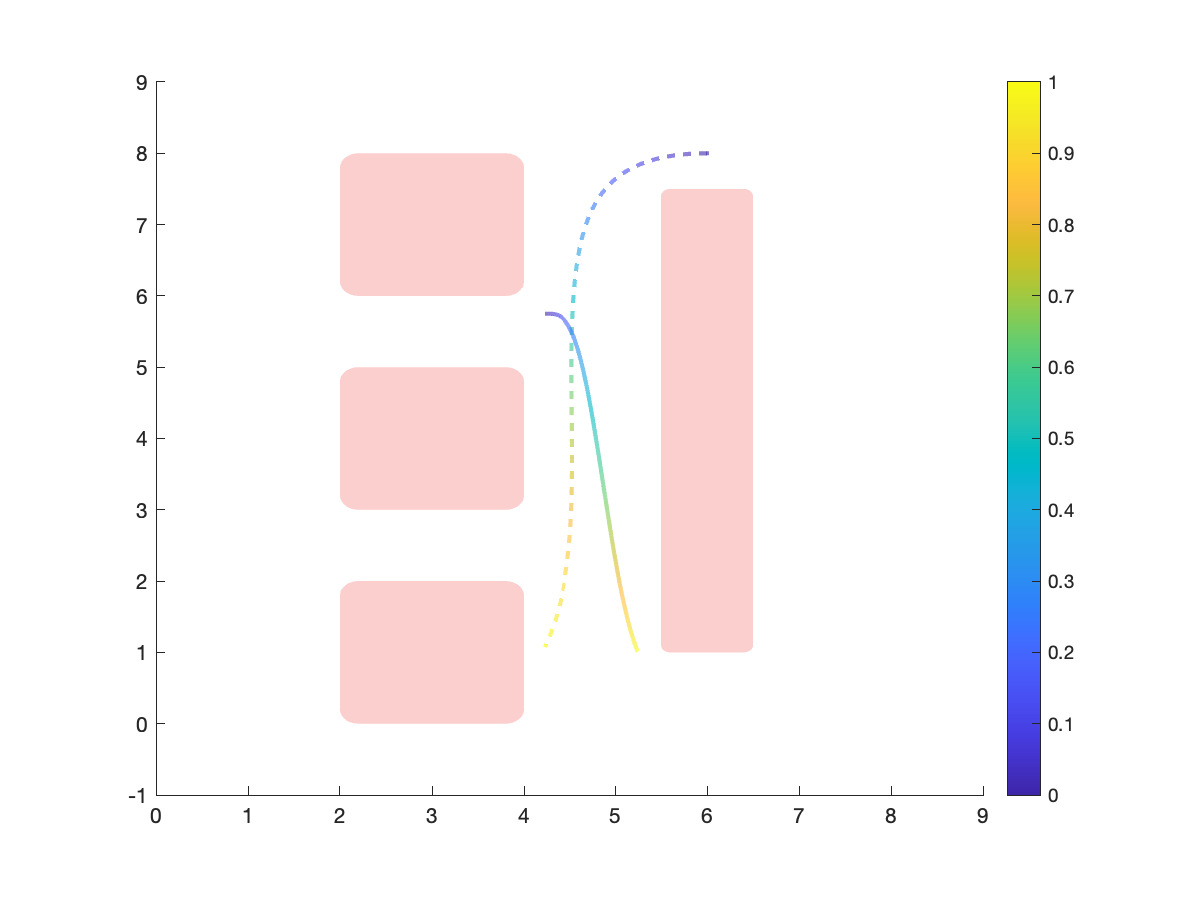
\includegraphics[width = 1.05\textwidth]{Figs/Chapter6/st_bezier_inital_2d.eps}}
		\end{minipage}
		\begin{minipage}{.45\linewidth}
			\centering
			\subfloat[]{%
				\label{FIG:ST-BEZIER-2D-INITIAL-B}%
				\includegraphics[width = 1.05\textwidth]{Figs/Chapter6/st_bezier_inital_distance_2d.eps}}
		\end{minipage}
	\end{center}
	\caption{Initial setting extrapolated from~\figref{FIG:ST-BEZIER-2D-SETTING}. In the left image, the two colliding pieces of
    trajectory are depicted with their behavior in time, normalized inside the interval $\lps 0,1 \rps$, while in the right image
    the blue line represents the agent-obstacle distance in time. The red dotted line, in the right image, is the chosen threshold
    for the minimum safe distance.}%
    \label{FIG:ST-BEZIER-2D-INITIAL}
\end{figure}
%%%%%%%%%%
With the previous analysis at hand, we propose here an optimisation-based approach to the replanning problem described
in~\secref{SEC:REPLANNING-PROBLEM-DEFINITION}, in the specific case where the obstacle trajectory $\rr_o \lp t \rp$ is known and
parameterised as a B\acuteacc ezier curve with control points $\cpoint_o^i$ for the path, and $\splinevar_o^i$ for the timing law.
In particular, let $\rr^j \lp t \rp$ the segment of~\eqqref{EQ:ST-SEPARATION-PIECEWISE} in (possible) collision with
the obstacle trajectory $\rr_o \lp t \rp$, then the problem of trajectory replanning can be solved as
\begin{equation}%
    \label{EQ:ST-SEPARATION-OPTIMISATION-PROBLEM}
    \begin{split}        
    \min_{
    \substack{\bs{\cpoint}_0, \dots, \bs{\cpoint}_{\order}; \\ \splinevar_0, \dots, \splinevar_{\order_{\splinevar}}}
    }
    & \loss
    \lp \bs{\cpoint}_0, \dots, \bs{\cpoint}_{\order}, \splinevar_0, \dots, \splinevar_{\order_{\splinevar}},
        \bs{\cpoint}^j_0, \dots, \bs{\cpoint}^j_{\order}, \splinevar^j_0, \dots, \splinevar^j_{\order_{\splinevar}} \rp \\
    \text{subj. to} \hspace{0.3cm} & \text{Continuity constraint}, \\
    & \text{Dynamical constraint}, \\
    & \text{Collision constraint},
    \end{split}
\end{equation}
with the constraints set depending on $\bs{\cpoint}^o_0, \dots, \bs{\cpoint}^o_{\order}, \splinevar^o_0, \dots, \splinevar^o_{\order_{\splinevar}}$.
The cost function $\loss \lp \cdot \rp$ can be chosen so as described in~\secref{SEC:REPLANNING-PROBLEM-DEFINITION}, recalling the
necessity to keep the replanned trajectory as close as possible to the original one
\begin{equation}%
    \label{EQ:ST-BEZIER-LOSS}
    \loss \lp \cdot \rp = \sum_{i=0}^{\order} \norm{\bs{\cpoint}_i - \bs{\cpoint}^j_i} + \sum_{i=0}^{\order_{\splinevar}} \lb \splinevar_i - \splinevar^j_i \rb,
\end{equation}
or so as described in~\secref{SEC:REPLANNING-OPTIMISATION}, including some trajectory regularisation terms.
In the following we briefly details and formulate the constraints in~\eqref{EQ:ST-SEPARATION-OPTIMISATION-PROBLEM}.
\begin{itemize}
    \item[\emph{Continuity}]\emph{constraint}.\\
    Belongs to this family of constraints all those conditions required to continuously connect the replanned trajectory segment with
    $\rr^{j-1}$ and $\rr^{j+1}$. In this context, we enforce continuity up to the third derivate, since higher order differentiations
    may complex the problem unnecessarily. Position continuity is easily obtained via control points matching as
    \begin{equation*}
        \begin{split}
            \splinevar_0 & = 0, \\
            \splinevar_{\order_{\splinevar}} & = 1, \\
            \rr_0 & = \rr_0^j, \\
            \rr_{\order} & = \rr_{\order}^j, \\
        \end{split}
    \end{equation*}
    where points denoted with apex $^j$ are the old control points.
    As regards velocity and acceleration continuity, we differentiate $\rr^j \lp t \rp$, with an eye to the composed stucture.
    \begin{equation*}
        \begin{split}
            \lp \rr_1 - \rr_0 \rp
            \lp \splinevar_1 - \splinevar_0 \rp & =
            \lp \rr^j_1 - \rr^j_0 \rp
            \lp \splinevar_1^j - \splinevar_0^j \rp, \\
            \lp \rr_{\order} - \rr_{\order-1} \rp
            \lp \splinevar_{\order_{\splinevar}} - \splinevar_{\order_{\splinevar}-1} \rp & =
            \lp \rr^j_{\order} - \rr^j_{\order-1} \rp
            \lp \splinevar_{\order_{\splinevar}}^j - \splinevar_{\order_{\splinevar}-1}^j \rp.
        \end{split}
    \end{equation*}
    \begin{equation*}
        \begin{matrix}
            \begin{matrix}
                \lp \rr_1 - \rr_0 \rp \lp \splinevar_2 - 2\splinevar_1 + \splinevar_0 \rp +
                \lp \rr_2 - 2\rr_1 + \rr_0 \rp \lp \splinevar_1 - \splinevar_0 \rp^2 = \\
                \lp \rr_1^j - \rr_0^j \rp \lp \splinevar_2^j - 2\splinevar_1^j + \splinevar_0^j \rp +
                \lp \rr_2^j - 2\rr_1^j + \rr_0^j \rp \lp \splinevar_1^j - \splinevar_0^j \rp^2,
            \end{matrix} \\
            \begin{matrix}
                \lp \rr_{\order} - \rr_{\order-1} \rp \lp \splinevar_{\order_{\splinevar}} - 2\splinevar_{\order_{\splinevar}-1} + \splinevar_{\order_{\splinevar}-2} \rp +
                \lp \rr_{\order} - 2\rr_{\order-1} + \rr_{\order-2} \rp \lp \splinevar_{\order_{\splinevar}} - \splinevar_{\order_{\splinevar}-1} \rp^2 = \\
                \lp \rr_{\order}^j - \rr_{\order-1}^j \rp \lp \splinevar_{\order_{\splinevar}}^j - 2\splinevar_{\order_{\splinevar}-1}^j + \splinevar_{\order_{\splinevar}-2}^j \rp +
                \lp \rr_{\order}^j - 2\rr_{\order-1}^j + \rr_{\order-2}^j \rp \lp \splinevar_{\order_{\splinevar}}^j - \splinevar_{\order_{\splinevar}-1}^j \rp^2.
            \end{matrix}
        \end{matrix}
    \end{equation*}

    \item[\emph{Dynamical}]\emph{constraint}.\\
    In the specific use case of quadcopter trajectory planning, differential flatness (\secref{SEC:DIFFERENTIAL-FLATNESS}) can be used to collapse
    the dynamics constraint to velocity and acceleration bounds.
    \begin{equation*}
        \begin{split}
            \order \order_{\splinevar} \lp \rr_{\splinevar_{i+1}} - \rr_{\splinevar_{i}} \rp / \lp T_{j+1} - T_j \rp & \le v_{\text{max}} \hspace{0.3cm} \forall i = 0, \dots, \order \order_{\splinevar}-1, \\
            \order \order_{\splinevar} \lp \order \order_{\splinevar} - 1 \rp \lp \rr_{\splinevar_{i+2}} - 2\rr_{\splinevar_{i+1}} + \rr_{\splinevar_{i}} \rp / \lp T_{j+1} - T_j \rp^2 & \le a_{\text{max}} \hspace{0.3cm} \forall i = 0, \dots, \order \order_{\splinevar}-2,
        \end{split}
    \end{equation*}
    with $\bs{\cpoint}_{\splinevar_{i}}$ be the $i$th control point of the composed curve~\eqref{EQ:ST-BEZIER-COMPOSITION-A}.
    Here we are exploiting the properties of closure with respect to composition and derivation, along with the convex hull containment one.
    In this context, as well as in the next collision constraint, the B\acuteacc ezier parameterisation plays a crucial role in
    simplifying the constraint formulation and dimensionality, leading to a manageable problem.

    \item[\emph{Collision}]\emph{constraint}.\\
    Finally, collision constraints are formulated as $n_{\text{c}}$ flght safe corridors for static obstacles avoidance,
    and as spatio-temporal distance for dynamic obstacle avoidance
    \begin{equation*}
        \begin{split}
            d_i & \ge d_{\text{safe}} \hspace{0.3cm} \forall i = 0, \dots, 2 \order \order_{\splinevar}, \\
            A^k \rr_i & \le b^k \hspace{0.3cm} \forall i = 0, \dots, \order, \hspace{0.3cm} \forall k = 0, \dots, n_{\text{c}}.
        \end{split}
    \end{equation*}
    In the aforementioned relation $d_i$ are the $2 \order \order_{\splinevar}$ control points defining the squared agent-obstacle
    distance, defined in~\eqqref{EQ:ST-BEZIER-COMPOSITION-F}, while $A^k$ and $b^k$ are $n_{\text{c}}$ convex polyhedra
    defining the safe regions free of static obstacles. In this setting, 
    \begin{equation*}
        \xset' = \bigcup_{k = 0}^{n_{\text{c}}} \left \{ \xx \in \R^{\dd{\xx}} : A^k \xx \le b^k \right \}.
    \end{equation*}
\end{itemize}
\begin{remark}
    The optimisation problem~\eqref{EQ:ST-SEPARATION-OPTIMISATION-PROBLEM} has been formulated for one agent only,
    colliding with a moving obstacle, the extension to the multi-agents case can be straightforwardly obtained by adding a new set
    of optimisation variables, describing the new agent trajectory.
\end{remark}

\subsection{Experimental Results}
%%%%%%%%%%
\begin{figure}[!t]
	\begin{center}
		\begin{minipage}{.45\linewidth}
			\centering
			\subfloat[]{%
				\label{FIG:ST-BEZIER-2D-U-RESULT-A}%
				\includegraphics[width = 1.05\textwidth]{Figs/Chapter6/st_bezier_u_opt_2d.eps}}
		\end{minipage}
		\begin{minipage}{.45\linewidth}
			\centering
			\subfloat[]{%
				\label{FIG:ST-BEZIER-2D-U-RESULT-B}%
				\includegraphics[width = 1.05\textwidth]{Figs/Chapter6/st_bezier_u_opt_distance_2d.eps}}
		\end{minipage}
	\end{center}
	\caption{Results of the proposed solution when used to optimise $\splinevar_i$ only.
    In the left image is depicted the same path as~\figref{FIG:ST-BEZIER-2D-INITIAL}, but with the new time behavior,
    normalized inside the interval $\lps 0,1 \rps$. The blue continuous line, in the right image, represents
    the new agent-obstacle distance, and the red dotted line is the fixed minimum safe distance.}%
    \label{FIG:ST-BEZIER-2D-U-RESULT}
\end{figure}
%%%%%%%%%%
%%%%%%%%%%
\begin{figure}[!t]
	\begin{center}
		\begin{minipage}{.45\linewidth}
			\centering
			\subfloat[]{%
				\label{FIG:ST-BEZIER-2D-PU-RESULT-A}%
				\includegraphics[width = 1.05\textwidth]{Figs/Chapter6/st_bezier_pu_opt_2d.eps}}
		\end{minipage}
		\begin{minipage}{.45\linewidth}
			\centering
			\subfloat[]{%
				\label{FIG:ST-BEZIER-2D-PU-RESULT-B}%
				\includegraphics[width = 1.05\textwidth]{Figs/Chapter6/st_bezier_pu_opt_distance_2d.eps}}
		\end{minipage}
	\end{center}
	\caption{Results of the proposed solution when used to optimise both $\bs{\cpoint}_i$ and $\splinevar_i$.
    In the left image is depicted the new path with the new time behavior, normalized inside the interval $\lps 0,1 \rps$.
    The blue continuous line, in the right image, represents the new agent-obstacle distance, and the red dotted line is the
    fixed minimum safe distance.}%
    \label{FIG:ST-BEZIER-2D-PU-RESULT}
\end{figure}
%%%%%%%%%%
%%%%%%%%%%
\begin{figure}[!t]
	\begin{center}
		\begin{minipage}{.45\linewidth}
			\centering
			\subfloat[]{%
				\label{FIG:ST-BEZIER-3D-INITIALY-A}%
				\includegraphics[width = 1.05\textwidth]{Figs/Chapter6/st_bezier_inital_setting_3d.eps}}
		\end{minipage}
		\begin{minipage}{.45\linewidth}
			\centering
			\subfloat[]{%
				\label{FIG:ST-BEZIER-3D-INITIAL-B}%
				\includegraphics[width = 1.05\textwidth]{Figs/Chapter6/st_bezier_inital_distance_3d.eps}}
		\end{minipage}
	\end{center}
	\caption{Initial three-dimensional testing scenario. In the left image, the two colliding pieces of
    trajectory are depicted with the considered collision sphere. In the right image, the blue line represents the
    agent-obstacle distance in time, and the red dotted line is the chosen threshold for the minimum safe distance.}%
    \label{FIG:ST-BEZIER-3D-INITIAL}
\end{figure}
%%%%%%%%%%
%%%%%%%%%%
\begin{figure}[!t]
	\begin{center}
		\begin{minipage}{.45\linewidth}
			\centering
			\subfloat[]{%
				\label{FIG:ST-BEZIER-3D-U-RESULT-A}%
				\includegraphics[width = 1.05\textwidth]{Figs/Chapter6/st_bezier_u_opt_3d.eps}}
		\end{minipage}
		\begin{minipage}{.45\linewidth}
			\centering
			\subfloat[]{%
				\label{FIG:ST-BEZIER-3D-U-RESULT-B}%
				\includegraphics[width = 1.05\textwidth]{Figs/Chapter6/st_bezier_u_opt_distance_3d.eps}}
		\end{minipage}
	\end{center}
	\caption{Results of the proposed solution when used to optimise $\splinevar_i$ only.
    In the left image is depicted the same path as~\figref{FIG:ST-BEZIER-3D-INITIAL}, but with the new time behavior,
    normalized inside the interval $\lps 0,1 \rps$. The blue continuous line, in the right image, represents
    the new agent-obstacle distance, and the red dotted line is the fixed minimum safe distance.}%
    \label{FIG:ST-BEZIER-3D-U-RESULT}
\end{figure}
%%%%%%%%%%
%%%%%%%%%%
\begin{figure}[!t]
	\begin{center}
		\begin{minipage}{.45\linewidth}
			\centering
			\subfloat[]{%
				\label{FIG:ST-BEZIER-3D-PU-RESULT-A}%
				\includegraphics[width = 1.05\textwidth]{Figs/Chapter6/st_bezier_pu_opt_3d.eps}}
		\end{minipage}
		\begin{minipage}{.45\linewidth}
			\centering
			\subfloat[]{%
				\label{FIG:ST-BEZIER-3D-PU-RESULT-B}%
				\includegraphics[width = 1.05\textwidth]{Figs/Chapter6/st_bezier_pu_opt_distance_3d.eps}}
		\end{minipage}
	\end{center}
	\caption{Results of the proposed solution when used to optimise both $\bs{\cpoint}_i$ and $\splinevar_i$.
    In the left image is depicted the new path with the new time behavior, normalized inside the interval $\lps 0,1 \rps$.
    The blue continuous line, in the right image, represents the new agent-obstacle distance, and the red dotted line is the
    fixed minimum safe distance.}%
    \label{FIG:ST-BEZIER-3D-PU-RESULT}
\end{figure}
%%%%%%%%%%
The proposed approach has been successfully applied in two different meaningful scenarios representing a two-dimensional
framework (\figref{FIG:ST-BEZIER-2D-INITIAL}), and a three-dimensional one (\figref{FIG:ST-BEZIER-3D-INITIAL}).
In both cases, the optimisation problem~\eqref{EQ:ST-SEPARATION-OPTIMISATION-PROBLEM} has been solved for $\splinevar_i$ only
and for both $\bs{\cpoint}_i$ and $\splinevar_i$. The obtained results are reported in Figures~\ref{FIG:ST-BEZIER-2D-U-RESULT}
and~\ref{FIG:ST-BEZIER-2D-PU-RESULT} for the two-dimensional case, and in Figures~\ref{FIG:ST-BEZIER-3D-U-RESULT}
and~\ref{FIG:ST-BEZIER-3D-PU-RESULT} for the three-dimensional one. In all figures the (a) image reports the resulting
trajectory along with its behavior in time, while image (b) depicts the agent-obstacle distance (blue line) with the fixed
minimum safe distance (red dotted line). In all simulations, we choose the loss function as in~\eqqref{EQ:ST-BEZIER-LOSS},
$d_{\text{safe}} = 0.25$, $v_{\text{max}} = 1.5m/s^2$, and $a_{\text{max}} = 0.5 m/s^2$.
The proposed solution succeeds, in each proposed scenario, to solve the trajectory replanning problem.
In the complete optimisation case, in Figures~\ref{FIG:ST-BEZIER-2D-PU-RESULT} and~\ref{FIG:ST-BEZIER-3D-PU-RESULT},
the algorithm is left free to trade-off between $\norm{\bs{\cpoint}_i - \bs{\cpoint}_i^j}$ and $\lb \splinevar_i - \splinevar_i^j \rb$
leading to a local optima with an higher final minimum distance.

%----------------------------------------------------------------------------------------
\section{Data-Driven Control Barrier Functions}
In this section, we detail a novel control-oriented approach to the replanning problem described in~\secref{SEC:REPLANNING-PROBLEM-DEFINITION},
focusing on the particular simplified case where only static obstacles may appear in a partially known environment.
The considered framework is well represented by~\eqqref{EQ:REPLANNING-OPTIMISATION-PROBLEM} with $\xset$ representing free and navigable
space, $\uset$ the set of all possible inputs, and $\xfun$ the considered system dynamics.
In this settings, the autonomous robot is pursuing an initial motion planned with only partial information about the surrounding
environment and concurrently is gathering information about it. The initial motion is then continuously refined with the collected
new information in order to ensure the robot safety at each time instant.
Motivated by this safety requirement, we ground the proposed solution on the notion of Control Barrier Function (CBF)~\cite{ames2016control}
which has been successfully demonstrated on many safety-critical applications~\cite{ames2016control, wang2017safe, hsu2015control}.
CBF applications ensure safety by enforcing the forward invariance of a \emph{safe set} described as a superlevel set of a candidate
function $\yfun$ which maps the system states to this notion of safety. In particular, the candidate function defines the hyper space
where the system is considered in a safe condition. Traditionally, these safety functions have been hand-designed. However,
depending on the application, designing such a candidate CBF is not straightforward in many practical settings. Consider, as an example,
the obstacle avoidance scenario, where the safe space is simply the free space, design the map $\yfun$ in this context requires
the complete environment knowledge, which is usually not completely a priori known.
Due to the aforementioned problem, we enforce the run-time adaptation of $\yfun$ via Gaussian process inference
exploiting real-time collected data, allowing for a constantly reshaping of the current motion with newly upcoming safe information.
The idea of learning the safe set from data is not new, in this sense Support Vector Machines (SVMs) were used in~\cite{srinivasan2020synthesis}
to parameterize CBFs with the help of sensor measurements. Neural networks were successfully used to regress the 
safety barrier function in~\cite{abate2020formal, zhao2020synthesizing, tsukamoto2020neural, gaby2021lyapunov}, while
a second-order cone program was formulated in~\cite{castaneda2021gaussian}, with GPs used for modeling the control input and the system uncertainties.
However, all these solutions are limited to offline training which limits their applicability in many practical scenarios.
Gaussian processes have been successfully used in~\cite{khan2021safety} and~\cite{khan2022gaussian} where the candidate function $\yfun$
is directly learned out of the collected data. The latter works, completely detach from a possible parameterised CBF and exploit the
GP regression in a completely data-driven scenario, without any a priori knowledge about the safe set.
However the quantity of collected data, required to build run-time the safe set, increases a lot with the system relative degree,
leading to poor, or even completely wrong, results.
Here we focused on the latter problem by formalising a new CBF-based solution that implements a Gaussian process regression 
requiring a limited number of samples whatever the system relative degree is. Then, the developed safety tool is successfully
implemented in the obstacle avoidance scenario.

We stress the fact that, unlike the approaches detailed in~\secref{SEC:REPLANNING-ALGORITHM} and~\secref{SEC:SPATION-TEMPORAL-SEPARATION},
the proposed solution does not require neither a resource consuming map building and maintenance, nor heavy 
random sampling procedure which may lead to very large set of samples, or possible trajectories, hard to handle.
The remain of this section unfolds as follow, in~\secref{SEC:CONTROL-BARRIER-FUNCTION} we briefly review key results on CBFs,~\secref{SEC:LEARNING-SAFE-SET}
describes a possible method to enforce the safe set learning, while in~\secref{SEC:PROPOSED-GAUSSIAN-CBF} and~\secref{SEC:CBF-RESULTS}
we formulate the proposed regulator and show the obtained results.

\subsection{Control Barrier Functions}%
\label{SEC:CONTROL-BARRIER-FUNCTION}
Consider the nonlinear control affine system
\begin{equation}%
    \label{EQ:CBF-INITIAL-SYSTEM}
    \begin{matrix}
        \dot{\xx} = \xfun \lp \xx \rp + \ufun \lp \xx \rp \uu, & \yy = \yfun \lp \xx \rp
    \end{matrix}
\end{equation}
where $\xx \in \R^{\dd{\xx}}$ is the system state, $\uu \in \uset \subset \R^{\dd{\uu}}$ is the input,
and $\yy \in \R^{\dd{\yy}}$ the measurable output. Moreover let $\xfun : \R^{\dd{\xx}} \mapsto \R^{\dd{\xx}}$
$\ufun : \R^{\dd{\xx}} \mapsto \R^{\dd{\xx} \times \dd{\uu}}$ and $\yfun : \R^{\dd{\xx}} \mapsto \R^{\dd{\yy}}$
Lipschitz continuous maps. Let the safety of~\eqref{EQ:CBF-INITIAL-SYSTEM} be encoded as the superlevel set
$\safeset$ of the smooth function $\yfun$
\begin{equation*}
    \safeset = \xset' = \left \{  \xx \in \R^{\dd{\xx}} : \yfun \lp \xx \rp \ge 0 \right \},
\end{equation*}
in this context we recall a couple of results from~\cite{xiao2019control, nguyen2016exponential, ames2016control}.
\begin{definition}%
    \label{DEF:CONTROL-BARRIER-FUNCTION}
    The map $\yfun \lp \xx \rp : \R^{\dd{\xx}} \mapsto \R^{\dd{\yy}}$ is defined as a Control Barrier Function (CBF),
    if there exists a class $\KK$ function $\alpha$, i.e. with the features (a) $\alpha \lp 0 \rp = 0$ and (b)
    $\alpha$ stricly increasing, such that the relation
    \begin{equation*}
        \sup_{\uu \in \uset} L_{\xfun} \yfun \lp \xx \rp + L_{\ufun} \yfun \lp \xx \rp \uu + \alpha \lp \yfun \lp \xx \rp\rp \ge 0,
    \end{equation*}
    holds for any $\xx \in \safeset$.
\end{definition}
In the previous definition the quantities $L_{\xfun} \yfun \lp \xx \rp$ and $L_{\ufun} \yfun \lp \xx \rp$ are the directional derivatives
of $\yfun$, along the flow defined by $\xfun$ and $\ufun$, respectively (along the literature called \emph{Lie derivatives}).
With the aforementioned definition at hand, we can easily enforce the system safety, which in this context implies no collisions,
by shaping the control input $\uu$ of~\eqref{EQ:CBF-INITIAL-SYSTEM} over the designed CBF in~\defref{DEF:CONTROL-BARRIER-FUNCTION}.
\begin{theorem}%
    \label{TH:SAFE-INVARIANCE}
    Given a nonlinear system as in~\eqqref{EQ:CBF-INITIAL-SYSTEM}, with a defined safe set $\safeset \subset \R^{\dd{\xx}}$,
    and a smooth control barrier function $\yfun \lp \xx \rp : \R^{\dd{\xx}} \mapsto \R^{\dd{\yy}}$, any Lipschitz continuous
    control law $\uu \lp t \rp \in \R^{\dd{\uu}}$ satisfying
    \begin{equation}%
        \label{EQ:CBF}
        L_{\xfun} \yfun \lp \xx \lp t \rp\rp + L_{\ufun} \yfun \lp \xx \lp t \rp\rp \uu \lp t \rp + \alpha \lp \yfun \lp \xx \lp t \rp\rp\rp \ge 0,
    \end{equation}
    for any $\xx \in \R^{\dd{\xx}}$, makes the safe set $\safeset$ forward invariant for~\eqref{EQ:CBF-INITIAL-SYSTEM}.
\end{theorem}
The reader can immediately conceive from~\thref{TH:SAFE-INVARIANCE} and~\defref{DEF:CONTROL-BARRIER-FUNCTION} the very limiting
requirement to have relative degree (here referred to as $\order$) equal to one, $\order = 1$.
For systems with $\order > 1$, we require an extension to the CBF notion defined so far. In particular, referring
to~\cite{nguyen2016exponential, xiao2019control}, let's introduce the concept of Exponential Control Barrier Function (ECBF).
\begin{definition}
    The smooth function $\yfun \lp \xx \rp: \R^{\dd{\xx}} \mapsto \R^{\dd{\yy}}$, with relative degree $\order$, is defined as an
    exponential control barrier function, if there exists a set of coefficients $ \Lambda \in \R^{\order}$ such that for any $\xx \in \R^{\dd{\xx}}$
    \begin{equation}%
        \label{EQ:ECBF}
        \sup_{\uu \in \uset} L^{\order}_{\xfun} \yfun \lp \xx \rp + L_{\ufun}L_{\xfun}^{\order-1} \yfun \lp \xx \rp \uu + \Lambda\T \HH \ge 0
    \end{equation}
    holds with $\HH = \lps \yfun \lp \xx \rp, L_{\xfun} \yfun \lp \xx \rp, \dots, L^{\order-1}_{\xfun} \yfun \lp \xx \rp\rps\T \in \R^{\order}$
    the Lie derivative vector for $\yfun$, and $\Lambda = \lps \lambda_0, \lambda_1, \dots, \lambda_{\order-1} \rps\T$ is a
    coefficient gain vector for $\HH$ which can be conputed via standard linear control techniques.
\end{definition}
The functions~\eqref{EQ:CBF} or~\eqref{EQ:ECBF} can then be combined with Quadratic Programs (QPs) to achieve safety constrained control,
in particular, for high relative degree systems, the forward invariance of the safe set $\safeset = \{ \xx \in \R^{\dd{\xx}} : \yfun \lp \xx \rp \ge 0\}$
can be enforced solving the following optimisation problem
\begin{equation}%
    \label{EQ:CBF-OPTIMISATION-PROBLEM}
    \begin{split}
        \uu = \arg \min_{v \in \uset} & \frac{1}{2} \norm{v - \uu\s} \\
        \text{subj. to} \hspace{0.2cm} & L_{\xfun}^{\order} \yfun \lp \xx \rp + L_{\ufun} L_{\xfun}^{\order-1} \yfun \lp \xx \rp v + \Lambda\T\HH \ge 0
    \end{split}
\end{equation}
with $\uu\s \in \R^{\dd{\uu}}$ previous planned control input, referred to as \emph{nominal input}.
\begin{remark}
    The problem~\eqref{EQ:CBF-OPTIMISATION-PROBLEM} resembles the replanning problem~\eqref{EQ:REPLANNING-OPTIMISATION-PROBLEM}
    borrowing the same loss and with the safe and dynamic constraints condensed in~\eqqref{EQ:ECBF}.
\end{remark}

\subsection{Learning the Safe Set}%
\label{SEC:LEARNING-SAFE-SET}
The major issue in using CBF to enforce safety lies in designing the candidate function $\yfun$, whose superlevel set
must encode all safe regions where the system state is allowed to evolve.
This problem is mainly present also in obstacle avoidance scenarios where the environment in not a priori known
making impossible the design of $\yfun$. To overcome this limitation,~\cite{khan2022gaussian} proposes to handle
the construction of $\yfun$ following a complete data-driven approach: the key idea was to model this unknown map
as a realisation of a Gaussian process. In particular, supposing to have access to a data-set
$\lp \bs{\xx}, \bs{\yy} \rp = \{ \lp \xx(t_1), \yy(t_1) \rp, \dots, \lp \xx(t_{N}), \yy(t_{N}) \rp \}$
of $N$ samples, with each pair $(\xx(t_h),$ $ \yy(t_h)) \in \R^{\dd{\xx}} \times \R^{\dd{\yy}}$ obtained as
$\yy(t_h) = \yfun \lp \xx(t_h) \rp + \noise(t_h)$ with $\noise(t_h) \sim \NN \lp 0, \nn I_{\dd{\yy}}\rp$
be a white Gaussian noise, then an approximation of $\yfun$ can be computed as
\begin{equation}%
   \label{EQ:CBF-GAUSSIAN-REGRESSION}
   \begin{split}
      \pmu \lp \xx \rp & = \kv \lp \xx \rp\T \lp\km + \nn I_{N}\rp^{-1}\bs{\yy}, \\
      \pvar \lp \xx \rp & = \kf \lp \xx, \xx \rp - \kv \lp \xx \rp \T \lp\km + \nn I_{N}\rp^{-1}\kv \lp \xx \rp,
   \end{split}
\end{equation}
where $\km \in \R^{N \times N}$ is the \textit{Gram matrix} whose $(k,h)$th entry is $\km_{k,h} = \kf \lp \bs{\xx}_k, \bs{\xx}_h \rp$,
with $\bs{\xx}_k$ the $k$th entry of $\bs{\xx}$, $\kv \lp \xx \rp \in \R^{N}$ is the kernel vector whose $k$th component is
$\kv_k \lp \xx \rp = \kf \lp \xx, \bs{\xx} \rp$, and $\kf \lp \xx, \xx' \rp$ is a custom kernel function~\cite{rasmussen2003gaussian}.
For further information about Gaussian regression and about the kernel structure the reader is referred to~\appref{SEC:GAUSSIAN-PROCESS-APPENDIX}.
Gaussian regression works by iteratively restricting the pool of possible functions, conditioning a prior Gaussian distribution on the
collected dataset. In this sense,~\eqqref{EQ:CBF-GAUSSIAN-REGRESSION} expresses the a posteriori mean ($\pmu$) and variance ($\pvar$)
computed after the collection of $N$ samples $\lp \bs{\xx}, \bs{\yy} \rp$.
In this context, the computed mean represents the ``best'' function approximation, while $\pvar$ quantifies the amount of uncertainties
affecting the current estimation, as it strongly depends on the amount of data collected near the evaluating point $\xx$.
Although the estimation $\pmu$ of $\yfun$ can be directly used inside the optimisation problem~\eqref{EQ:CBF-OPTIMISATION-PROBLEM}
in place of $\yfun$, we should be careful of possible errors and uncertainties in the reconstructed approximation as a wrong value of
$\pmu$ may make condition~\eqref{EQ:ECBF} holds even in unsafe conditions.
As a matter of fact, evaluating an unknown function out of data may lead to wrong results, especially if the collected data are
poorly informative or very scattered.
To overtake this particular problem,~\cite{khan2022gaussian} proposed a re-reading of the candidate function keeping into consideration
also the provided a posteriori variance of the current estimation $\pmu$, thus $\yfun$ has been reformulated as
\begin{equation*}
    h_{\text{GP}}\lp \xx \rp = \pmu \lp \xx \rp - \rho \pvar \lp \xx \rp,
\end{equation*}
with $\rho \in \R^{+}$ a tunable value, leading to the new optimisation problem
\begin{equation*}
    \begin{split}
        \uu = & \arg \min_{v \in \uset} \frac{1}{2} \norm{v - \uu\s} \\
        & \text{s.t.} \hspace*{0.2cm} L_{\xfun}^{\order} \yfun_{\text{GP}}\lp \xx \rp +
                                      L_{\ufun} L_{\xfun}^{\order-1} \yfun_{\text{GP}} \lp \xx \rp v + \Lambda\T\HH \ge 0.
    \end{split}
\end{equation*}
The aforementioned approach is very promising under the perspective of adapt CBF tools to a very large number of use cases, especially
when an analytical formulation of $\yfun$ is not accessible, but results to be very poor practically when dealing with systems with
high relative degrees $\order > 1$ because of loss of information during Gaussian process differentiation~\cite{holsclaw2013gaussian}.
Furthermore, the parameter $\rho$ results to be the key to obtain good performances even with $\order = 1$, thus a very careful tuning
is required to make the algorithm works correctly.
The aforementioned problems motivated our research in the field of Gaussian control barrier functions toward more general and resilient
solutions, especially tailored for high relative degree systems.

\subsection{Proposed Gaussian Control Barrier Function}%
\label{SEC:PROPOSED-GAUSSIAN-CBF}
%%%%%%%%%%
\begin{figure}[!t]
	\begin{center}
		\begin{minipage}{.45\linewidth}
			\centering
			\subfloat[]{%
				\label{FIG:CBF-RESULTS-COMPARISON-A}%
				\includegraphics[width = 1.05\textwidth]{Figs/Chapter6/cbf_0505.png}}
		\end{minipage}
		\begin{minipage}{.45\linewidth}
			\centering
			\subfloat[]{%
				\label{FIG:CBF-RESULTS-COMPARISON-B}%
				\includegraphics[width = 1.05\textwidth]{Figs/Chapter6/cbf_0505_gp.png}}
		\end{minipage}
		\begin{minipage}{.45\linewidth}
			\centering
			\subfloat[]{%
				\label{FIG:CBF-RESULTS-COMPARISON-C}%
				\includegraphics[width = 1.05\textwidth]{Figs/Chapter6/cbf_0505_gp_hg.png}}
		\end{minipage}
	\end{center}
	\caption{Comparison between (a) classic ECBF, (b) GP-CBF proposed by~\cite{khan2022gaussian}, and (c) GP-CBF proposed here.
    In image (a) the safe set is designed using the complete knowledge of the environment, while in images (b) and (c) the
    candidate function is reconstructed run-time using the collected sensor data.}%
    \label{FIG:CBF-RESULTS-COMPARISON}
\end{figure}
%%%%%%%%%%
The proposed regulator reads as
\begin{equation}%
    \label{EQ:CBF-PROPOSED-OBSERVER}
    \dot{\zz} = A\zz + B \lp L_{\xfun} \pmu \lp \xx \rp + L_{\ufun} \pmu \lp \xx \rp \uu \rp + G \lp l \rp H \lp \yy - C\zz \rp,
\end{equation}
with output
\begin{equation}%
    \label{EQ:CBF-PROPOSED-OPTIMISATION-PROBLEM}
    \begin{split}
        \uu = \arg \min_{v \in \uset} & \frac{1}{2} \norm{v - \uu\s} + L_{\ufun} \pvar \lp \xx \rp v \\
        \text{subj. to} \hspace{0.2cm} & L_{\xfun} \pmu \lp \xx \rp + L_{\ufun} \pmu \lp \xx \rp v + \Lambda\T\HH \ge 0.
    \end{split}
\end{equation}
As emerges from~\eqqref{EQ:CBF-PROPOSED-OBSERVER}, the proposed regulator consists in a standard high-gain observer
with $A$, $B$, and $C$ matrices in prime form
\begin{equation*}
    \begin{matrix}
        A =
        \begin{pmatrix}
            0_{(\order-1)\dd{\yy} \times \dd{\yy}} & I_{(\order-1)\dd{\yy}} \\
            0_{\dd{\yy} \times \dd{\yy}} & 0_{\dd{\yy} \times (\order-1)\dd{\yy}}
        \end{pmatrix}, &
        B =
        \begin{pmatrix}
            0_{(\order-1)\dd{\yy} \times \dd{\yy}} \\
            I_{\dd{\yy}}
        \end{pmatrix},
    \end{matrix}
    \end{equation*}
    \begin{equation*}
    C =
    \begin{pmatrix}
        I_{\dd{\yy}} & 0_{\dd{\yy} \times (\order-1)\dd{\yy}}
    \end{pmatrix},
\end{equation*}
and $G(l) = \text{diag} \lp l I_{\dd{\yy}}, l^{2} I_{\dd{\yy}}, \dots, l^{r} I_{\dd{\yy}} \rp$,
$H = \text{diag} \lp H_1, \dots, H_r \rp$, and $H_i = \text{diag} \big( h^1_i, \dots$ $\dots, h^{\dd{\yy}}_i \big)$ with
$\{h_{1}^j, h_{2}^j, \dots, h_{r+1}^j\}$ for all $j = 1, \dots, \dd{\yy}$ coefficients of a Hurwitz polinomial,
where $l \in \R_{>0}$ is a control parameter.
In this context, the proposed observer is meant to directly reconstruct $L_{\xfun}^{\order-1} \yfun$, that in turn is
feeded back to a Gaussian regressor which outputs an analytical and differentiable estimate
\begin{equation*}
	\pmu \lp \xx \rp = \kv \lp \xx \rp\T \lps \km + \nn I_N \rps^{-1} \bs{\zz},
\end{equation*}
with $\bs{\zz}$ extracted from the recostructed data-set
\begin{equation*}
    \lp \bs{\xx}, \bs{\zz} \rp = \{ \lp \xx(t_1), \zz_{\order-1}(t_1) \rp, \dots, \lp \xx(t_{N}), \zz_{\order-1}(t_{N}) \rp \}.
\end{equation*}
The regressed directional derivate is then used to reconstruct the observer consistency term~\cite{buisson2021joint}.
Equation~\eqref{EQ:CBF-PROPOSED-OPTIMISATION-PROBLEM} reformulates the one-relative-degree problem~\eqref{EQ:CBF-OPTIMISATION-PROBLEM}
in this particular framework. Note that the used candidate function does not take into account any uncertainties in the
retrieved estimation, which in turn are encode inside the loss function as $L_{\ufun} \pvar \lp \xx \rp v$, with
$\pvar$ the a posteriori Gaussian variance
\begin{equation*}
	\pvar \lp \xx \rp = \kf \lp \xx,\xx \rp - \kv \lp \xx \rp\T \lps \km + \nn I_N \rps^{-1} \kv \lp \xx \rp.
\end{equation*}
\begin{remark}
    Although the new loss proposed in~\eqqref{EQ:CBF-PROPOSED-OPTIMISATION-PROBLEM} presents a slightly different structure
    with respect to classical CBF formulation~\eqref{EQ:CBF-OPTIMISATION-PROBLEM} and with respect to the formulated
    problem in~\secref{SEC:REPLANNING-PROBLEM-DEFINITION}, it still succeed in solving the obstacle avoidance problem as the
    collision is encoded as optimisation hard constraint. Moreover, minimise $L_{\ufun} \pvar \lp \xx \rp v$ directly
    implies a minimisation of the induced uncertainties affecting $\pmu$ as the agent is forced to navigate toward already
    visited frontiers. As a matter of fact, the aforementioned term comes out from~\eqqref{EQ:ECBF} cosidering
    $\yfun = \pmu + \pvar$
    \begin{equation*}
        \sup_{\uu \in \uset} L_{\xfun} \yfun \lp \xx \rp + L_{\ufun} \yfun \lp \xx \rp v + \Lambda\T\HH \ge 0,
    \end{equation*}
    \begin{equation*}
        L_{\xfun} \lp \pmu \lp \xx \rp + \pvar \lp \xx \rp \rp + L_{\ufun} \lp \pmu \lp \xx \rp + \pvar \lp \xx \rp \rp v.
    \end{equation*}
    We stress the fact that encoding an uncertainties term inside the cost formulation drops the necessity to introduce a weight $\rho$
    inside the candidate function, as done in~\cite{khan2022gaussian}, whose wrong tuning may degrade the algorithm performance.
\end{remark}
\begin{remark}
    The proposed solution~\eqref{EQ:CBF-PROPOSED-OBSERVER}-\eqref{EQ:CBF-PROPOSED-OPTIMISATION-PROBLEM} is well suited for
    high relative degree applications as the regressed map $\pmu$ is differentiated only once, leading to a very few loss of
    information. In the context of Gaussian process, the latter property implies the possibility to keep the value of $N$ low,
    leading to light real-time training procedures.
\end{remark}
We conclude this section by recalling two basic properties which the regressor should undergo to make the proposed solution works 
correctly. We stress the fact that the assumptions reported below are not restrictive under the practical point of view, and can be
easily satisfied by all commonly used kernels. The following assumptions are borrowed from~\cite{buisson2021joint}.
\begin{assumption}%
    $\pmu$ is Lipschitz continuous with Lipschitz constant $L_{\pmu}$, and its norm is bounded by $\pmu_{\text{max}}$.
 \end{assumption}
 \begin{assumption}%
    The kernel function $\kf(\cdot, \cdot)$ is Lipschitz continuous with constant $L_{\kf}$, with a locally Lipschitz derivative of constant $L_{d\kf}$,
    and its norm is bounded by $\kf_{\text{max}}$.
 \end{assumption}

\subsection{Experimental Results}%
\label{SEC:CBF-RESULTS}
%%%%%%%%%%
\begin{figure}[!t]
	\begin{center}
		\begin{minipage}{.45\linewidth}
			\centering
			\subfloat[]{%
				\label{FIG:CBF-RESULTS-FAIL-A}%
				\includegraphics[width = 1.05\textwidth]{Figs/Chapter6/cbf_0505_gp_hg_test_1.png}}
		\end{minipage}
		\begin{minipage}{.45\linewidth}
			\centering
			\subfloat[]{%
				\label{FIG:CBF-RESULTS-FAIL-B}%
				\includegraphics[width = 1.05\textwidth]{Figs/Chapter6/cbf_0505_gp_hg_test_2.png}}
		\end{minipage}
	\end{center}
	\caption{Results obtained in challenging environments when applying the proposed approach without
    taking into account estimation uncertainties carried by $\pvar$. As the reader can observe, the proposed solution
    does not make the agent colliding, but can stuck it close to obstacles.}%
    \label{FIG:CBF-RESULTS-FAIL}
\end{figure}
%%%%%%%%%%
%%%%%%%%%%
\begin{figure}[!t]
	\begin{center}
		\begin{minipage}{.45\linewidth}
			\centering
			\subfloat[]{%
				\label{FIG:CBF-RESULTS-WIN-A}%
				\includegraphics[width = 1.05\textwidth]{Figs/Chapter6/cbf_0505_gp_hg_norm_test_1.png}}
		\end{minipage}
		\begin{minipage}{.45\linewidth}
			\centering
			\subfloat[]{%
				\label{FIG:CBF-RESULTS-WIN-B}%
				\includegraphics[width = 1.05\textwidth]{Figs/Chapter6/cbf_0505_gp_hg_norm_test_2.png}}
		\end{minipage}
	\end{center}
	\caption{Results obtained in challenging environments when applying the overall proposed approach.
    The encoded uncertainties via $\pvar$ drive the agent in regions with low uncertainties, making the final solution
    working in all cases.}%
    \label{FIG:CBF-RESULTS-WIN}
\end{figure}
%%%%%%%%%%
The proposed approach has been applied to a synthetic scenario and tested against the classical ECBF, where the safe
set design has been made using the full knowledge about the navigating environment, and the state-of-the-art
Gaussian-based CBF proposed by~\cite{khan2022gaussian}. In both the learning techniques, the training data are collected
real time, while the agent is moving inside the environment.
The testing scenario (see~\figref{FIG:CBF-RESULTS-COMPARISON}) is equal in all experiments and consists of four shpere-like
obstacles with random positions and four surrounding walls. The agent is modeled a simple double integrator with acceleration
as control input, while the nominal control input $\uu\s$ consists in a straight line from the initial to the goal position.
In this settings, the candidate function $\yfun$ is modeled as the distance from the closest obstacle, following the
Euclidean Signed Distance Field (ESDF) principle~\cite{oleynikova2017voxblox}.
The obtained results are reported in Figures~\ref{FIG:CBF-RESULTS-COMPARISON},~\ref{FIG:CBF-RESULTS-FAIL}, and~\ref{FIG:CBF-RESULTS-WIN}.
In particular,~\figref{FIG:CBF-RESULTS-COMPARISON} depicts a comparison between the classical ECBF, the GP-CBF proposed by~\cite{khan2022gaussian},
and our approach when applied in the same settings described above. The classical ECBF, designed on the complete knowledge of the
environment, always succeeds in safely steering the agent to the goal and its results are kept here as a baseline to follow in the case
where no prior information about the obstacles is provided. As the reader can see, from~\figref{FIG:CBF-RESULTS-COMPARISON},
the approach proposed by~\cite{khan2022gaussian} sometimes fails, especially in highly cluttered environment, while our approach
always wins. To highlight the fundamental role which plays the regulariser $L_{\ufun} \pvar \lp \xx \rp v$
in~\eqref{EQ:CBF-PROPOSED-OPTIMISATION-PROBLEM}, we reported here two simulations in Figures~\ref{FIG:CBF-RESULTS-FAIL} and~\ref{FIG:CBF-RESULTS-WIN}
where the proposed approach is applied without and with the regularisation term. In particular, in~\figref{FIG:CBF-RESULTS-FAIL}
the term is not present, while in~\figref{FIG:CBF-RESULTS-WIN} the optimisation problem is solved with the proposed complete loss function.
It is worth to remark how in both cases the agent does not collide with obstacles, but in the first reported simulations the high uncertainties
affecting the estimated candidate function made the agent stuck near to obstacles.

%----------------------------------------------------------------------------------------
\section{Contributions}
In this chapter we reviewed and discussed the problem of real-time trajectory replanning in front of new environmental information.
The chapter develops firstly by reviewing a state-of-the-art solution to the problem at hand, adapted, re-implemented and tested in the
specific case of the Leonardo drone contest. The selected solution performed well and succeed in replanning jerk-continuous trajectories
well suited for quadcopter navigation. Then, two novel solutions have been described and analyzed, one primarily focused on the specific
case of moving obstacles and multi-agent scenarios, and the second one focused on static environments.
The proposed flow embraces a research direction especially focused on numeric and system theory-oriented solutions where the possibility
of success can be easily assessed via analysis tools commonly used in the system theory field.
As a future research direction, we will continue to follow this idea and try to encode Lyapunov theory in novel trajectory
plaNning, or replanning, techniques yielding to very high reliable and robust solutions.

%------------------------------------------------
\cleardoublepage % Empty page before the start of the next part

%------------------------------------------------
% \ctparttext{Some info here.}
\part{Adaptive Nonlinear Output Regulation}

\chapter{Data-Driven Nonlinear Regulation}%
\label{CH:DATA-DRIVEN-REGULATION}
In this chapter, we collect the basic notions behind the concept of output regulation and data-driven output regulation for nonlinear systems.
The section unfolds as follows, first we introduce, in the simplest possible terms, the problem of output regulation in the
nonlinear context, with an eye to the taxonomy usually adopted in this field.
Then, the next part is devoted to briefly presenting the state-of-the-art of the most consolidated approaches to
the emergent field of \emph{adaptive} nonlinear output regulation and how these techniques can be extended via learning tools, obtaining
a highly robust and flexible solution, able to adapt to a very large class of systems.
The same concepts, notation, and results can also be found in~\cite*{bin2019class, bin2020model, bin2020approximate, gentilini2022adaptive, gentilini2022data}
thus we refer the reader to these works for the complete analysis of the presented results.

%----------------------------------------------------------------------------------------
\section{The Framework of Output Regulation}%
\label{SEC:FRAMEWORK-OUTPUT-REGULATION}
Consider a continuous-time nonlinear system of the form
\begin{equation}%
    \label{EQ:GENERAL-OR-SYSTEM}
    \begin{split}
        \dot{\xx} & = \xfun \lp \ww, \xx, \uu \rp, \\
        \yy & = \yfun \lp \ww, \xx \rp,
    \end{split}
\end{equation}
with state $\xx \in \R^{\dd{\xx}}$, control input $\uu \in \R^{\dd{\uu}}$, measured output $\yy \in \R^{\dd{\yy}}$, and
with $\ww \in \R^{\dd{\ww}}$ exogenous signal generated by an exosystem of the form
\begin{equation}%
    \label{EQ:GENERAL-EXOSYSTEM}
    \dot{\ww} = \wfun \lp \ww \rp.
\end{equation}
The exogenous signal can be treated, in this context, as references to be tracked or disturbances to be rejected.
For this purpose, associated to~\eqqref{EQ:GENERAL-OR-SYSTEM}, there is a set of $\dd{\ee} > 0$ regulation errors
\begin{equation*}
    \ee = \efun \lp \ww, \xx \rp.
\end{equation*}
In this framework, we define the problem of $\eps$-approximate output regulation as the problem to find
an output feedback regulator of the form
\begin{equation}%
    \label{EQ:GENERAL-OR-REGULATOR}
    \begin{split}
        \dot{\xx}_c & = \rfun \lp \xx_c, \yy \rp, \\
        \uu & = \actfun \lp \xx_c, \yy \rp,
    \end{split}
\end{equation}
possibly $\eps$-dependent, with state $\xx_c \in \R^{\dd{\xx_c}}$, such that:
\begin{itemize}
    \item[\emph{Stability.}] The origin of the interconnection between~\eqqref{EQ:GENERAL-OR-SYSTEM} and~\eqqref{EQ:GENERAL-OR-REGULATOR},
    with $\ww = 0$, is asymptotically stable with a domain of attraction $\xset \times \xset_c \in \R^{\dd{\xx}} \times \R^{\dd{\xx_c}}$
    that is an open neighborhood of the origin.
    \item[\emph{Boundedness.}] There exists $\wset \in \R^{\dd{\ww}}$ such that the closed-loop system is uniformly bounded from
    $\wset \times \xset \times \xset_c$.
    \item[\emph{Regulation.}] Each solution to the closed-loop system originating in $\wset \times \xset \times \xset_c$ satisfies
    \begin{equation*}
        \limsup_{t \rightarrow \infty} \| \ee \lp t \rp \| \le \eps.
    \end{equation*}
\end{itemize}
If $\xset$ coincides with $\R^{\dd{\xx}}$, we say that the problem is solved \emph{globally}, otherwise we say that the problem
is solved \emph{locally}. If given each $\xset \subset \R^{\dd{\xx}}$ it is possible to find a possibly $\xset$-dependent regulator 
that solves the problem in $\xset$, we say that the problem is solved \emph{semi-globally}.
If $\eps = 0$, we refer to the problem as the \emph{asymptotic} output regulation problem, while we talk about
\emph{practical} regulation problem whenever, given any $\eps > 0$, there exists a regulator that solves the $\eps$-approximate
output regulation problem. An anchor point in the solution of the above problem is represented by the
steady-state trajectories $\lp \xx^{*}(t), \uu^{*}(t) \rp$, solution of the so-called \emph{regulator equations}
\begin{equation}%
    \label{EQ:GENERAL-REGULATOR-EQUATIONS}
    \begin{split}
        \dot{\ww} & = \wfun \lp \ww \rp, \\ 
        \dot{\xx}^{*} & = \xfun \lp \ww, \xx^{*}, \uu^{*} \rp, \\
        0 & = \efun \lp \ww, \xx^{*} \rp,
    \end{split}
\end{equation}
with $\xx^{*}$ representing the ideal state trajectory associated with a zero regulation error and $\uu^{*}$
the associated input (often referred to as ``the friend'' of $\xx^{*}$).
Regulator structures proposed in the nonlinear context are typically composed of two units, an internal model unit,
and a stabilising unit, with a neat, albeit limiting in many contexts, ``role'' conferred on the two at the design stage:
the former is designed to generate the steady state input $\uu^{*}$ required to keep the error at zero in steady state,
while the latter is designed to steer the closed-loop trajectories of the system to $\xx^{*}$.
What makes the design problem particularly challenging is, of course, the fact that $\lp \xx^{*}(t), \uu^{*}(t) \rp$
are unknown as the initial conditions of~\eqqref{EQ:GENERAL-REGULATOR-EQUATIONS} are such.
Moreover, the sufficient conditions under which asymptotic regulation is ensured are typically expressed by equations
whose analytic solution becomes a hard task even for ``simple'' problems. Moreover, even if a regulator can be constructed,
asymptotic regulation remains a fragile property that is lost at front of slightest plant's or exosystem's perturbation.
The aforementioned problems motivate the researcher to move toward more robust solutions, introducing the concept of adaptive regulation.
In the following we briefly present the two main adaptive approaches to nonlinear regulation designs that have influenced this thesis most strongly,
then we try to extend them via non-supervised learning techniques, to adapt the proposed structure on an ideally infinite class of systems.
The reported regulators embed two different internal models, being a ``post-processing'' the first one and a ``pre-processing'' the second one,
but both apply to multivariable systems. The proposed construction is not ``friend-centric'' but rather it is based on a
``qualitative'' information on the ideal error-zeroing steady state.

%----------------------------------------------------------------------------------------
\section{Identification-Based Post-Processing Internal Model}
\label{SEC:POST-PROCESSING}
In this section, we focus on a subclass of the general regulation problem presented in~\secref{SEC:FRAMEWORK-OUTPUT-REGULATION}
by considering continuous-time nonlinear systems of the form
\begin{equation}%
   \label{EQ:POSTP-FRAMEWORK}
   \begin{split}
      \dot{\zz} &= \zfun(\xx ,\ww) + \zin(\xx, \ww) \uu, \\
      \dot{\chain} &= F \chain + H \last, \\
      \dot{\last} &= \qfun(\xx ,\ww) + \bfun(\xx ,\ww) \uu, \\
      \ee &= C \chain, \hspace{0.5cm} \yy = \text{col}(\chain, \last),
   \end{split}
\end{equation}
in which $\zz \in \R^{\dd{\zz}}$, $\yy \in \R^{\dd{\yy}}$, $\ee \in \R^{\dd{\ee}}$, $\chain \in \R^{\dd{\ee}}$, and,
$\uu \in \R^{\dd{\uu}}$ with $\dd{\uu} \ge \dd{\ee}$. The entire stack of states is denoted here by $\xx = \text{col}(\zz, \chain, \last)$.
Moreover, $\chain = \text{col}(\chain^1, \dots, \chain^{\dd{\ee}})$, with $\chain^i \in \R^{n_{\chain}^i}$, $i = 1, \dots, \dd{\ee}$,
and $\sum_{k=1}^{\dd{\ee}} n_{\chain}^k = n_{\chain}$. The exogenous signal $\ww \in \R^{\dd{\ww}}$ is generated by an exosystem
of the same form of~\eqqref{EQ:GENERAL-EXOSYSTEM}. The matrices $F \in \R^{n_{\chain} \times n_{\chain}}$,
$H \in \R^{n_{\chain} \times \dd{\ee}}$, and $C \in \R^{\dd{\ee} \times n_{\chain}}$ are defined as a block-diagonal matrices with entries
\begin{equation*}
   \begin{matrix}
      F_i =
      \begin{pmatrix}
         0_{(n_{\chain}^i-1) \times 1} & I_{n_{\chain}^i - 1} \\
         0 & 0_{1 \times (n_{\chain}^i-1)}
      \end{pmatrix}, &
      H_i =
      \begin{pmatrix}
         0_{(n_{\chain}^i-1) \times 1} \\ 1
      \end{pmatrix},
   \end{matrix}
\end{equation*}
\begin{equation*}
   C_i =
   \begin{pmatrix}
      1 & 0_{1 \times (n_{\chain}^i-1)}
   \end{pmatrix}.
\end{equation*}
Equation~\eqref{EQ:POSTP-FRAMEWORK} frames the problem of output regulation on a particular class of systems that embraces
a large number of use-cases addressed in literature. In particular, note that all systems presenting \textit{(a)} a well-defined vector
relative degree and admitting a canonical normal form, or that are \textit{(b)} strongly invertible and feedback linearisable,
with respect to the pair $\lp \uu, \ee \rp$, fit inside the proposed framework.
The regulator presented in this section is based on the following standing assumptions (see~\cite[Assumption~A1,~A2]{bin2019class}).
\begin{assumption}%
   There exist $\beta_0 \in \KL$, $\alpha_0 > 0$ and, for each solution $\ww$ of~\eqref{EQ:GENERAL-EXOSYSTEM},
   there exist $\zz\s : \R_{\ge 0} \mapsto \R^{\dd{\zz}}$ and $\uu\s : \R_{\ge 0} \mapsto \R^{\dd{\uu}}$ fulfilling
   \begin{equation}%
      \label{EQ:POSTP-REGULATOR-EQUATIONS}
      \begin{split}
         \dot{\zz}\s & = \zfun(\ww, \xx\s) + \zin(\ww, \xx\s)\uu\s, \\
         0 & = q(\ww, \xx\s) + \bfun(\ww, \xx\s)\uu\s,
      \end{split}
   \end{equation}
   where $\xx\s = \lp\zz\s, 0, 0\rp$, and for all $t > 0$ the following holds
   \begin{equation*}
      \lb \zz(t) - \zz\s(t) \rb \le \beta_0\lp\lb \zz(0) - \zz\s(0) \rb, t\rp + \alpha_0 \lb \lp\chain, \last\rp \rb_{\lps0,t\rp}.
   \end{equation*}
\end{assumption}
\begin{assumption}%
   There exists a full-rank matrix $\LL \in \R^{\dd{\uu} \times \dd{\ee}}$ such that the matrix $\bfun(\ww, \xx)\LL$ is bounded, and
   \begin{equation*}
      \LL\T \bfun(\ww, \xx)\T + \bfun(\ww, \xx) \LL \ge I_{\dd{\ee}}
   \end{equation*}
   holds for all $(\ww, \xx) \in \R^{\dd{\ww}} \times \R^{\dd{\xx}}$, and the map
   \begin{equation*}
      (\ww,\xx) \mapsto (\bfun(\ww, \xx)\LL)^{-1} q(\ww, \xx)    
   \end{equation*}
   is Lipschitz.
\end{assumption}
Equations~\eqref{EQ:POSTP-REGULATOR-EQUATIONS} are the specialisation of the regulator equations~\eqref{EQ:GENERAL-REGULATOR-EQUATIONS}
in this non-equilibrium context. As a consequence of the latter assumption, $\uu\s$ in~\eqref{EQ:POSTP-REGULATOR-EQUATIONS} is given by
\begin{equation*}
   \uu\s = - \bfun \lp \ww, \xx\s \rp\T \lp \bfun \lp \ww, \xx\s \rp \bfun \lp \ww, \xx\s \rp\T \rp^{-1} q \lp \ww, \xx\s \rp.
\end{equation*}
In this framework,~\cite{bin2019class} proposes a post-processing internal model of the form
\begin{equation*}%
   \begin{matrix}
      \dot{\im} = \imfun(\im) + Ge, & \im \in \R^{d \dd{\ee}},
   \end{matrix}
\end{equation*}
with $d \in \N$, $\im = \lp \im_1, \dots, \im_d \rp\T$, $\im_i \in \R^{\dd{\ee}}$, and
\begin{equation}%
   \label{EQ:POSTP-INTERNAL-MODEL}
   \begin{matrix}
      \Phi(\im) = 
      \begin{pmatrix}
         \im_2 \\ \vdots \\ \im_d \\ \imfunsingle(\im, \param)
      \end{pmatrix}, &
      G =
      \begin{pmatrix}
         g h_1 I_{\dd{\ee}} \\ g^2 h_2 I_{\dd{\ee}} \\ \vdots \\ g^d h_d I_{\dd{\ee}}
      \end{pmatrix}.
   \end{matrix}
\end{equation}
In the aforementioned definition, the coefficients $h_i$, with $i = 1, \dots, d$, are fixed so that the polynomial
$s^d + h_1s^{d-1}+\cdots+h_{d-1}s+h_d$ is Hurwitz, $g > 0$ is a parameter to be designed, and
$\imfunsingle: \R^{d \dd{\ee}} \times \R^{\dd{\param}} \mapsto \R^{\dd{\ee}}$ is a function to be fixed and $\param \in \R^{\dd{\param}}$,
with $\dd{\param} \in \N$, is an adaptive parameter generated by the identifier subsystem, whose dynamics is described by
\begin{equation}
    \begin{split}%
      \label{EQ:POSTP-GENERAL-IDENTIFIER}
      \dot{\id} & = \idfun \lp \id, \im, \ee \rp, \\
      \param & = \idout \lp \id \rp,
    \end{split}
\end{equation}
in which $\idfun : \idset \times \R^{d \dd{\ee}} \times \R^{\dd{\ee}} \mapsto \idset$ and $\idout : \idset \mapsto \R^{\dd{\param}}$, with $\idset$ a 
normed vector space of finite dimension, have to be fixed. Finally, the static stabiliser control action is chosen as
\begin{equation*}%
   \uu = \LL(K_{\chain}\chain + K_{\last}\last + K_{\im}\im_1 + K_{\ww} \nu(\xx\s, \ww)),
\end{equation*}
where the matrices $K_{\chain}$, $K_{\last}$, and $K_{\im}$ take the form
\begin{equation*}
   \begin{matrix}
      K_{\chain}(l,\delta) = lK(\delta), & K_{\last}(l) = -lI_{\dd{\ee}}, & K_{\im}(l,\delta) = lK(\delta)C\T,
   \end{matrix}
\end{equation*}
with $K(\delta) = \text{blkdiag} \lp K^1(\delta), \dots, K^{\dd{\ee}}(\delta)\rp$, where
\begin{equation*}
   K^i(\delta) = - \lp 
   \begin{matrix} 
      c_1^i \delta^{n_{\chain}^i} & c_2^i \delta^{n_{\chain}^i - 1} & c_{n_{\chain}^i}^i \delta 
   \end{matrix} \rp,
\end{equation*}
for $i = 1, \dots, \dd{\ee}$, in which the coefficients $c_j^i$ are chosen so that the polynomial
$s^{n_{\chain}^i} + c^i_{n_{\chain}^i}s^{n_{\chain}^i - 1} + \cdots + c_2^i s + c_1^i$, $i = 1, \dots, \dd{\ee}$,
is Hurwitz, and $l, \delta > 0$ are design parameters to be fixed.
Note that the matrix $K_{\ww}$ and the function $\nu(\cdot, \cdot)$ are left as a degree of freedom.
Indeed these quantities can be used to represent possible feedforward contributions added by the
designer employing knowledge about $\ww$ and $\xx\s$ (Equation~\eqref{EQ:POSTP-REGULATOR-EQUATIONS}).
The degrees of freedom left to be fixed at this stage are the dimension $d$ and function $\imfunsingle$ of the internal model unit,
the data $\lp \idset, \dd{\param}, \idfun, \idout \rp$ of the identifier, and the control parameters $g, l$, and $\delta$.
A key step in the regulator synthesis is the choice of the internal model~\eqref{EQ:POSTP-INTERNAL-MODEL}
and of its adaptation through the design of the identifier~\eqref{EQ:POSTP-GENERAL-IDENTIFIER}.
This should be chosen in order to achieve small, possibly zero, asymptotic regulation error,
in spite of uncertainties involving the regulation equations and the system dynamics.
From~\eqqref{EQ:POSTP-INTERNAL-MODEL} we can write
\begin{equation}%
   \label{EQ:POSTP-REGULATION-ERROR}
   \ee \lp t \rp = \lp h_d g^d \rp^{-1} \lp \dot{\im}_d \lp t \rp - \imfunsingle \lp \im \lp t \rp, \param \lp t \rp \rp \rp.
\end{equation}
The proposed design strategy chooses $\lp d, \imfunsingle \rp$ and the identifier pivoting around the idea that $\dot{\im}_d \lp t \rp - \imfunsingle \lp \im \lp t \rp, \param \lp t \rp \rp$
can be interpreted as a prediction error attained by the model $\imfunsingle$ in relating the next derivative $\dot{\im}_d \lp t \rp$
to the previous derivatives $\im \lp t \rp$, and that, by minimising this prediction error, the actual regulation error is also minimised due to~\eqref{EQ:POSTP-REGULATION-ERROR}.
In this context, the problem of choosing $\lp d, \imfunsingle \rp$ is treated as an identification problem, where $\imfunsingle \lp \im, \param \rp$
is referred to as \emph{prediction model} and the set
\begin{equation*}
   \MM = \left\{ \imfunsingle \lp \im, \param \rp : \param \in \R^{\dd{\param}} \right\}
\end{equation*}
of all the possible candidate models as the corresponding \emph{model set}.
The selection of such quantities must be grounded on some preliminary knowledge about the class of signals to
$\dot{\im}_d$ and $\im$ are expected to belong. In this context, the steady-state signals $\lp \xx\s, \uu\s \rp$
resulting from the regulator equations are the anchor point on which that knowledge can be drawn.
The original work~\cite{bin2019class} provides a constructive procedure to design the internal model quantities,
as well as the identifier functions, showing how approximate
regulation can be attained, thus for more details the reader is referred to it.

%----------------------------------------------------------------------------------------
\section{Adapting the Post-Processing Internal Model}
All the approaches that assume to known the membership model of the friend have the 
disadvantage of limiting the \textit{class of friends} which we can deal with, leading to a
degraded performance in all those cases in which the steady-state signals $\lp \xx\s, \uu\s \rp$ are highly uncertain
and the chosen class $\MM$ is inadequate to represent the ideal function $\imfunsingle\s$.
Unlike previous works in this field, we dropped the assumption of $\imfunsingle$ belonging to a given model set on
behalf of a more general and less conservative hypothesis.
In particular, we let such a function be of whatever shape, with the only constraint to be \textit{sufficiently smooth}.
In this respect, we refer to $\imfunsingle \lp \im, \param \rp$ with $\imfunsingle \lp \im \rp$, to highlight the generality
of the proposed framework, being $\imfunsingle$ not parameterised by any $\param$.
In view of the latter, we recall~\cite[Assumption~A3]{bin2019class} under which the asymptotic stability results can be drawn.
\begin{assumption}%
	\label{ASSUM:INTERNAL-MODEL}
	The map $\imfunsingle \lp \im \rp$ is Lipschitz and differentiable with a locally Lipschitz derivative,
	and the Lipschitz constants do not depend on $\delta$ and $l$.
	Moreover, there exists a compact set $H\s \subset \R^{\dd{\ee}} \times \R^{d \dd{\ee}}$, independent from $\delta$ and $l$,
	such that every solution of
	\begin{equation*}
		\dot{\im} = \imfun(\im) + Ge,
	\end{equation*}
	satisfies $\lp \im_d\s(t), \im\s(t) \rp \in H\s$ for all $t \in \R_{\ge 0}$.
\end{assumption}

\subsection{Gaussian Process Regression}%
\label{SEC:OR-POST-PROCESSING-GAUSSIAN-INFERENCE}
The key idea behind the proposed approach dwells in modeling the unknown function $\imfunsingle$ as the realization of a Gaussian process.
GPs are function estimators widely used because of the flexibility they offer in modeling nonlinear maps directly out from the collected data~\cite{rasmussen2003gaussian}.
A GP model is fully described by a mean function $\prior: \R^{d \dd{\ee}} \mapsto \R^{\dd{\ee}}$ and a covariance function (aka \textit{kernel})
$\kf: \R^{d \dd{\ee}} \times \R^{d \dd{\ee}} \mapsto \R^{\dd{\ee}}$. Whereas there are many possible choices of mean and covariance functions, in this work we keep 
the formulation of $\kf$ general, with the only constraint expressed by~\assumptionref{ASSUM:K-CONTINUOUS-BOUNDED} below.
Yet we force, without loss of generality, $\prior \lp \im \rp = 0_{\dd{\ee}}$ for any $\im$. Thus we assume that
\begin{equation*}
   \imfunsingle \lp \im \rp \sim \GP \lp 0, \kf \lp \cdot, \cdot \rp \rp.
\end{equation*}
Supposing to have access to a data-set
$\lp \stx, \sty \rp = \{ \lp \im(t_1), \dot{\im}_d(t_1) \rp, \dots$
$\dots, \lp \im(t_{N}), \dot{\im}_d(t_{N}) \rp \}$ with each pair
$\lp \im(t_h), \dot{\im}_d(t_h) \rp \in \R^{d \dd{\ee}} \times \R^{\dd{\ee}}$ obtained as
$\dot{\im}_d(t_h) = \imfunsingle(\im(t_h)) + \noise(t_h)$ with
$\noise(t_h) \sim \NN \lp 0, \nn I_{\dd{\ee}}\rp$ be a white Gaussian noise, then the posterior distribution of $\imfunsingle$ given the data-set is still
a Gaussian process with mean $\pmu$ and variance $\pvar$ given by~\cite{rasmussen2003gaussian}
\begin{equation}%
   \label{EQ:OR-POST-PROCESSING-GP-POSTERIOR}
   \begin{split}
      \pmu \lp \im \rp & = \kv \lp \im \rp\T \lp\km + \nn I_{N}\rp^{-1}\sty, \\
      \pvar \lp \im \rp & = \kf \lp \im, \im \rp - \kv \lp \im \rp \T \lp\km + \nn I_{N}\rp^{-1}\kv \lp \im \rp,
   \end{split}
\end{equation}
where $\km \in \R^{N \times N}$ is the \textit{Gram matrix} whose $(k,h)$th entry is $\km_{k,h} = \kf \lp \stx_k, \stx_h \rp$,
with $\stx_k$ the $k$th entry of $\stx$, and $\kv \lp \im \rp \in \R^{N}$ is the kernel vector whose $k$th component is $\kv_k \lp \im \rp = \kf \lp \im, \stx_k \rp$.
The problem of inferring an unknown function $\imfunsingle$ from a finite set of data can be seen as a special case of \textit{ridge regression} where the
prior assumptions (mean and covariance) are encoded in terms of \emph{smoothness} of $\pmu$.
In particular, let $\HH$ be a RKHS associated with the kernel function $\kf$, then the function $\imfunsingle$ can be infered by minimizing the functional
\begin{equation*}
   \loss = \frac{\lambda_s}{2} \norm{\pmu}^2_{\HH} + Q \lp \sty, \pmu \lp \stx \rp \rp,
\end{equation*}
where the first term plays the role of \textit{regularizer} and represents the smoothness assumptions on $\pmu$
as encoded by a suitable RKHS, while the second one represents the data-fit term assessing the quality of the prediction
$\pmu \lp \stx \rp$ with respect to the observed data $\sty$~\cite{rasmussen2003gaussian}.
According to the \textit{representer theorem}~\cite{o1986automatic}, each minimizer $\pmu \in \HH$ of $\loss$ takes the form  
$\pmu \lp \im \rp = \kv \lp \im \rp\alpha$. In the particular case in which $Q\lp\sty, \pmu\lp\stx\rp\rp$ corresponds to a negative log-likelihood
of a Gaussian model with variance $\nn$, namely
\begin{equation*}
   Q\lp\sty, \pmu\lp\stx\rp\rp = \frac{1}{2 \nn} \norm{\sty - \pmu\lp\stx\rp}^2_2,
\end{equation*}
the value of $\alpha$ recovers the expression in Equation~\eqref{EQ:OR-POST-PROCESSING-GP-POSTERIOR} as
\begin{equation*}
   \alpha = \lp\km + \nn I\rp^{-1}\sty.
\end{equation*}
From now on we suppose that the following standing assumptions hold (see~\cite[Assumption~2,~Assumption~3]{buisson2021joint})
\begin{assumption}%
   \label{ASSUM:MU-CONTINUOUS-BOUNDED}
   $\pmu$ is Lipschitz continuous with Lipschitz constant $L_{\im}$, and its norm is bounded by $\pmu_{\text{max}}$.
\end{assumption}
\begin{assumption}%
   \label{ASSUM:K-CONTINUOUS-BOUNDED}
   The kernel function $\kf(\cdot, \cdot)$ is Lipschitz continuous with constant $L_{\kf}$, with a locally Lipschitz derivative of constant $L_{d\kf}$,
   and its norm is bounded by $\kf_{\text{max}}$.
\end{assumption}

Although any kernel fulfilling~\assumptionref{ASSUM:K-CONTINUOUS-BOUNDED} can be a valid candidate, in the following,
we exploit the commonly adopted \textit{squared exponential kernel} as prior covariance function, which can be expressed as
\begin{equation}%
   \label{EQ:OR-POST-PROCESSING-EXPONENTIAL-KERNEL}
   \kf\lp\im, \im'\rp = \np \exp\lp -\lp\im - \im'\rp\T \Lambda^{-1}  \lp\im - \im'\rp \rp
\end{equation}
for all $\im, \im' \in \R^{d\dd{\ee}}$, where $\Lambda = \text{diag}(2\lambda_{\im_1}^2, \dots, 2\lambda_{\im_{d\dd{\ee}}}^2)$, $\lambda_{\im_{i}} \in \R_{>0}$ is
known as \textit{characteristic length scale} relative to the $i$th signal, and $\np$ is usually called
\textit{amplitude}~\cite{rasmussen2003gaussian}.
We conclude this section by stating a constructive assumption, on which the main contribution of this chapter is built.
\begin{lemma}%
   \label{LEMMA:RKHS-LIPSCHITZ}
   Let $\HH$ be a RKHS induced by a positive-definite kernel $\kf$, satisfying~\assumptionref{ASSUM:K-CONTINUOUS-BOUNDED}, and let $f \in \HH$,
   then $f$ is Lipschitz continuous with constant $L_{f} = \norm{f}_{\HH} c_{\HH} L_{\kf}$, where $c_{\HH}$ is a positive real constant.
   \graffito{The $L^2$ and $\HH$ norms, being the latter induced by a positive definite kernel, are equivalent with constant $c_{\HH}$
   (see~\cite{dai2014scalable} for further details).}
\end{lemma}
\begin{proof}
   \begin{equation*}
      \begin{split}
         \lb f(x) - f(x') \rb & = \lb \langle f, \kf(\cdot, x) \rangle_{\HH} - \langle f, \kf(\cdot, x') \rangle_{\HH} \rb \\
         & = \lb \langle f, \kf(\cdot, x)-\kf(\cdot, x') \rangle_{\HH} \rb \\
         & \le \norm{ f }_{\HH} \norm{ \kf(\cdot, x)-\kf(\cdot, x') }_{\HH} \\
         & \le \norm{ f }_{\HH} c_{\HH} \norm{ \kf(\cdot, x)-\kf(\cdot, x') } \\
         & \le \norm{ f }_{\HH} c_{\HH} L_{\kf} \norm{ x-x' } \\
         & \le L_{f} \norm{ x-x' }
      \end{split}
   \end{equation*}
\end{proof}
\begin{assumption}%
   \label{ASSUM:RKHS-BELONGING}
   The map $\imfunsingle$ belongs to the RKHS associated to the kernel function $\kf(\cdot, \cdot)$ in Equation~\eqref{EQ:OR-POST-PROCESSING-EXPONENTIAL-KERNEL}.
\end{assumption}
It is worth noting that the first statement of~\assumptionref{ASSUM:INTERNAL-MODEL} is implied by~\assumptionref{ASSUM:RKHS-BELONGING} by means of
\lemref{LEMMA:RKHS-LIPSCHITZ}.

\subsection{Gaussian Process-based Adaptive Regulation}%
\label{SEC:OR-POST-PROCESSING-LEARNING-DRIVEN-REGULATION}
%%%%%%%%%%
\begin{figure}[!t]
	\centering
	\includegraphics[width=0.8\textwidth]{Figs/Chapter8-9/postprocessing_vtol.png}
	\caption{The vertical takeoff and landing aircraft considered in numerical simulations.}
	\label{FIG:OR-POSTPROCESSING-VERTICAL-TOL}
\end{figure}
%%%%%%%%%%
The proposed regulator reads as follows
\begin{equation}%
   \label{EQ:OR-POST-PROCESSING-OVERALL-REGULATOR}
   \begin{split}
      &
      \begin{cases}
         \dot{\clock} & = 1 \\
         \dot{\im} & = \imfun(\im, \pmu(\im, \id, \alpha, \clock)) + Ge \\
         \dot{\obs}_1 & = \obs_2 - m_1 \obsgain(\obs_1 - \im_d) \\
         \dot{\obs}_2 & = \dot{\pmu}(\im, \id, \alpha, \clock) - m_2 \obsgain^2 (\obs_1 - \im_d) \\
         \dot{\id} & = 0 \\
      \end{cases} \\
      & \lp \im, \obs_1, \obs_2, \id, \clock \rp \in \CC, \\
      &
      \begin{cases}
         \clock^{+} & = 0 \\
         \im^{+} & = \im \\
         \obs_1^{+} & = \obs_1 \\
         \obs_2^{+} & = \obs_2 \\
         \id^{+} & = \lp S \otimes I_{p}\rp \id + \lp B \otimes I_{p}\rp \begin{bmatrix} \im & \obs_2 & \clock \end{bmatrix}\T \\
      \end{cases} \\
      & \lp \im, \obs_1, \obs_2, \id, \clock \rp \in \DD, \\
   \end{split}
\end{equation}
in which $\alpha = \gamma \lp \id \rp \in \R^{N \times N}$, $p = d\dd{\ee} + \dd{\ee} + 1$,
$\lp \obs_1, \obs_2 \rp \in \R^{\dd{\ee}} \times \R^{\dd{\ee}}$, and $\id \in \R^{\dd{\id}}$ with $\dd{\id} = pN$.
The matrices $S \in \R^{N \times N}$ and $B \in \R^{N}$ have the ``shift'' form
\begin{equation*}
   \begin{matrix}
      S = 
      \begin{pmatrix}
         0_{(N-1) \times 1} & I_{N-1} \\
         0 & 0_{1 \times (N-1)}
      \end{pmatrix}, &
      B = 
      \begin{pmatrix}
         0_{(N-1) \times 1} \\ 1
      \end{pmatrix},
   \end{matrix}
\end{equation*}
while $\imfun$ and $G$ have the same structure described by Equation~\eqref{EQ:POSTP-INTERNAL-MODEL},
$\CC = \{ \lp \im, \obs_1, \obs_2, \id, \clock \rp \in \R^{d\dd{\ee}} \times \R^{\dd{\ee}} \times \R^{\dd{\ee}} \times \idset \times \R_{\ge 0} : \pvar \lp \im, \id, \alpha, \clock \rp \le \pvar_{\text{thr}} \}$
represents the flow set, and
$\DD = \{ \lp \im, \obs_1, \obs_2, \id, \clock \rp \in \R^{d\dd{\ee}} \times \R^{\dd{\ee}} \times \R^{\dd{\ee}} \times \idset \times \R_{\ge 0} : \pvar \lp \im, \id, \alpha, \clock \rp \ge \pvar_{\text{thr}} \}$
is the jump set, with $\pvar_{\text{thr}}$ arbitrary. The functions $\pmu \lp \im, \id, \alpha, \clock \rp$ and $\pvar \lp \im, \id, \alpha, \clock \rp$
represent the a posteriori GP estimated mean and variance after the collection of $N$ samples, and $\idset \subseteq \R^{N \dd{\id}}$.
The proposed regulator is composed of \textit{(a)} a purely continuous-time subsystem $\lp \im, \obs_1, \obs_2 \rp$ whose dynamics depends
on $\id$ and $\alpha$ that are constant during flow, \textit{(b)} a purely discrete-time subsystem $\id$ updated ad each jump time,
and \textit{(c)} a hybrid clock $\clock$. Note that, due to the definition of the sets $\CC$ and $\DD$ the jumping law is not directly
related to the clock variable $\clock$, thus at the moment it is not clear if~\eqref{EQ:OR-POST-PROCESSING-OVERALL-REGULATOR} suffers from
\textit{zeno} or \textit{chattering} issues.
The subsystem $\im$ plays the role of internal model unit, and it is taken of the same form as~\eqref{EQ:POSTP-INTERNAL-MODEL}.
The subsystem $\lp \obs_1, \obs_2 \rp$ plays the role of \textit{observer} of the quantity $\dot{\im}_d$ required to build the 
data-set and not directly available. The dynamic equation of $\lp \dot{\obs}_1, \dot{\obs}_2 \rp$ follows the canonical high-gain construction
with the coefficients $m_1, m_2 > 0$ arbitrary and $\obsgain > 0$ left as a design parameter.
The quantities $\lp \obs_2, \im \rp$ act as proxy for the ideal $\lp \dot{\im}_d\s, \im\s \rp$ required to build an approximation of $\imfunsingle\s$;
$\lp \obs_2, \im \rp$ are thus feeded to the discrete-time GP regressor represented by the subsystem $\id$ and by the properly defined
functions $\lp \pmu, \pvar, \gamma \rp$. In particular, denoting $\cvar = \col{\im, \clock}$, the latter functions read as
\begin{equation*}
   \begin{split}
      \pmu \lp \cvar \rp & = \kv \lp \cvar \rp\T \gamma \lp \id \rp \boldsymbol{\obs_2}, \\
      \pvar \lp \cvar \rp & = \kf \lp \cvar, \cvar \rp - \kv \lp \cvar \rp\T \gamma \lp \id\rp \kv \lp \cvar \rp, \\
      \gamma \lp \id \rp & = \lp \km + \nn I_{N} \rp^{-1},
   \end{split}
\end{equation*}
where $\kv$ and $\km$ are defined as in~\secref{SEC:OR-POST-PROCESSING-GAUSSIAN-INFERENCE},
with the only differency that the kernel function $\kf$ has been enhanced by adding a dependency from $\clock$.
In this context, Equation~\eqref{EQ:OR-POST-PROCESSING-EXPONENTIAL-KERNEL} takes the form
\begin{equation*}
   \begin{split}
      \kf \lp \cvar_i, \cvar_j \rp = \pvar_p \exp & \lp - \lp \im_i - \im_j \rp\T \Lambda^{-1} \lp \im_i - \im_j \rp \rp \\
        & \exp \lp -\sum_{k = \min(i, j)}^{\max(i, j)} \norm{\frac{\clock_k}{2 \lambda_{\clock}}} \rp \text{if } \cvar_i, \cvar_j \in \bcvar,
   \end{split}
\end{equation*}
\begin{equation}%
   \label{EQ:OR-POST-PROCESSING-EXPONENTIAL-KERNEL-TIME-2}
   \begin{split}
      \kf(\cvar, \cvar_j) = \pvar_p \exp & \lp - \lp \im - \im_j \rp\T \Lambda^{-1} \lp \im - \im_j \rp \rp \\
        & \exp \lp - \frac{\clock}{2 \lambda_{\clock}^2} + \sum_{k = j}^{m} \norm{\frac{\clock_k}{2 \lambda_{\clock}}} \rp \text{if } \cvar \notin \bcvar, \cvar_j \in \bcvar,
   \end{split}
\end{equation}
where $\lambda_{\clock}$ is a parameter to be tuned and the quantity $\lp \bcvar, \boldsymbol{\obs_2} \rp$ represents the data-set
constructed as discussed in~\secref{SEC:OR-POST-PROCESSING-GAUSSIAN-INFERENCE} extended with the sampled clock $\clock$,
and stored, as a state variable, inside the shift register $\id$.
The addition of the clock as independent variable inside the GP regression is the key to obtain a good estimation of $\imfunsingle$ starting from
the noisy proxy $\lp \obs_2, \im \rp$. This choice is motivated by the fact that the introduction of $\clock$ allows us to shape $\pmu$
through the parameter $\lambda_{\clock}$ whose inverse value can be interpreted as a \textit{forgetting factor}, commonly used in identification.

The design parameters $\lp g, l, \delta, \rho \rp$ in~\eqref{EQ:OR-POST-PROCESSING-OVERALL-REGULATOR} can be chosen so that the closed-loop
system has an asymptotic regulation error bounded by a function of the best attainable prediction, namely
\begin{equation*}
   \lim_{t \to \infty} \sup \norm{\ee(t)} = c_{\ee} \lim_{t \to \infty} \sup \norm{\dot{\im}_d\s(t) - \pmu(\im\s(t))},
\end{equation*}
with $c_{\ee}$ constant that depends on the chosen parameters.
Such a results directly follows from the adaptation of the arguments reported by~\cite{bin2019class} and~\cite{bin2020approximate}
in the specific case in which~\eqref{EQ:OR-POST-PROCESSING-OVERALL-REGULATOR} satisfies a set of properties known as \textit{identifier requirements}.
The following results are instrumental to verify that the proposed regulator fits inside the same framework of~\cite{bin2019class} and~\cite{bin2020approximate}.
\begin{lemma}%
   \label{LEMMA:DWELL-TIME}
   Let Assumptions~\ref{ASSUM:INTERNAL-MODEL},~\ref{ASSUM:MU-CONTINUOUS-BOUNDED}, and~\ref{ASSUM:K-CONTINUOUS-BOUNDED} hold.
   Moreover, suppose that the chosen $\pvar_{\text{thr}}$ satisfies
   \begin{equation}%
      \label{EQ:OR-POSTP-SIGMA-CONDITION}
      \frac{\np \nn}{\np + \nn} < \pvar_{\text{thr}} < \np,
   \end{equation}
   then any solution $\lp \im, \obs_1, \obs_2, \id, \clock \rp$ of~\eqref{EQ:OR-POST-PROCESSING-OVERALL-REGULATOR} originating from the set
   $\chi_0 = \{ \lp \im, \obs_1, \obs_2, \id, \clock \rp \in \R^{d\dd{\ee}} \times \R^{\dd{\ee}} \times \R^{\dd{\ee}} \times \idset \times \R_{\ge 0} : \clock = 0\}$
   satisfies a dwell time condition in the sense of~\cite{hespanha1999stability}, and a reverse dwell time condition in
   the sense of~\cite{hespanha2005input}.
\end{lemma}
\begin{proof}
   Using the same arguments proposed by~\cite{hespanha2005input}, we shape the proof to show the existence of $\overline{\text{T}}$ and $\underline{\text{T}}$
   such that $\CC \subseteq \{ \lp \im, \obs_1, \obs_2, \id, \clock \rp \in \R^{d\dd{\ee}} \times \R^{\dd{\ee}} \times \idset \times \R^{mp} \times \R_{\ge 0} : 0 \le \clock \le \overline{\text{T}} \}$
   and $\DD \subseteq \{ \lp \im, \obs_1, \obs_2, \id, \clock \rp \in \R^{d\dd{\ee}} \times \R^{\dd{\ee}} \times \idset \times \R^{mp} \times \R_{\ge 0} : \underline{\text{T}} \le \clock \le \overline{\text{T}} \}$.
   First note that, in view of~\assumptionref{ASSUM:INTERNAL-MODEL}, from the definition of kernel in~\eqref{EQ:OR-POST-PROCESSING-EXPONENTIAL-KERNEL-TIME-2},
   the value of $\pvar \lp \im, \id, \alpha, \clock \rp$ reaches $\np$ as long as $t$ goes to infinty, i.e.
   \begin{equation}%
      \label{EQ:OR-POSTP-SIGMA-LIMIT}
      \lim_{t \to \infty} \pvar \lp \im(t), \id(t), \alpha(t), \clock(t) \rp = \np.
   \end{equation}
   Recalling $\cvar = \col{\im, \clock}$, then the flow and jump dynamics of $\pvar$ are described by
   \begin{equation}%
      \label{EQ:OR-POSTP-SIGMA-FLOW}
      \begin{split}
         \dot{\lp \pvar\rp} & = \dot{\cvar}\T \lp \frac{d \kf \lp \cvar, \cvar \rp}{d \cvar} - 2 \frac{d \kv(\cvar)}{d \cvar}\T \gamma \lp \id \rp \kv \lp \cvar \rp \rp \\
         & = - 2 \dot{\cvar}\T \frac{d \kv \lp \cvar \rp}{d \cvar}\T \gamma \lp \id \rp \kv \lp \cvar \rp,
      \end{split}
   \end{equation}
   when $\lp \im, \obs_1, \obs_2, \id, \clock\rp \in \CC$, and
   \begin{equation}%
      \label{EQ:OR-POSTP-SIGMA-JUMP}
      \lp \pvar \rp^+ = \kf \lp \cvar^+, \cvar^+ \rp - \kv \lp \cvar^+ \rp \gamma \lp \id^+ \rp \kv \lp \cvar^+ \rp,
   \end{equation}
   when $\lp \im, \obs_1, \obs_2, \id, \clock\rp \in \DD$.
   The existence of $\overline{\text{T}}$ follows from~\eqref{EQ:OR-POSTP-SIGMA-LIMIT} and the second inequality of~\eqref{EQ:OR-POSTP-SIGMA-CONDITION},
   in particular by choosing $\pvar_{\text{thr}} < \np$, since $\pvar \to_{\clock \to \infty} \np$, there exists a real value $\overline{\text{T}}$
   such that $\pvar \ge \pvar_{\text{thr}}$ for any $\clock \ge \overline{\text{T}}$. This ensures persistency of jump intervals.
   Consider now Equations~\eqref{EQ:OR-POSTP-SIGMA-FLOW} and~\eqref{EQ:OR-POSTP-SIGMA-JUMP}, the flow dynamics $\dot{\lp \pvar \rp}$ results to be a continous function
   being it a product of Lipschitz functions (Assumptions~\ref{ASSUM:INTERNAL-MODEL},~\ref{ASSUM:MU-CONTINUOUS-BOUNDED},~\ref{ASSUM:K-CONTINUOUS-BOUNDED}).
   Moreover, its norm can be upper bounded as
   \begin{equation*}
      \norm{\dot{\lp \pvar\rp}} \le 2 \norm{\dot{\cvar}} \norm{\frac{d \kv \lp \cvar \rp}{d \cvar}} \norm{\gamma \lp \id \rp} \norm{\kv \lp \cvar \rp},
   \end{equation*}
   with $\dot{\cvar} = \lps \im_2, \dots, \im_d, \imfunsingle \lp \im \rp, 1 \rps\T$.
   Since during flow the function $\kf$ takes the form of~\eqref{EQ:OR-POST-PROCESSING-EXPONENTIAL-KERNEL-TIME-2}, rewriting the latter as
   \begin{equation*}
      \kf \lp \cvar, \cvar_j \rp = \np \exp\lp -\lp \cvar-\cvar_j \rp\T \bar{\Lambda}^{-1} \lp \cvar-\cvar_j \rp\rp,
   \end{equation*}
   the quantity 
   \begin{equation*}
      \frac{d \kv \lp \cvar \rp}{d \cvar} =
      \begin{bmatrix}
		-\kf \lp \cvar, \cvar^1 \rp \bar{\Lambda}^{-1} \lp \cvar - \cvar^1 \rp \\
		-\kf \lp \cvar, \cvar^2 \rp \bar{\Lambda}^{-1} \lp \cvar - \cvar^2 \rp \\
		\vdots \\
		-\kf \lp \cvar, \cvar^m \rp \bar{\Lambda}^{-1} \lp \cvar - \cvar^m \rp
      \end{bmatrix},
   \end{equation*}
   where $\cvar^i$ denotes the $i$th training point stored inside $\id$, and with $\bar{\Lambda}$ properly defined.
   \assumptionref{ASSUM:INTERNAL-MODEL} ensures $\norm{\dot{\cvar}} \le l_{\cvar}$, with $l_{\cvar}$ dependent on the chosen $H\s$,
   while~\assumptionref{ASSUM:K-CONTINUOUS-BOUNDED} ensures boundedness of $\gamma \lp \id \rp$ and $\kv \lp \cvar \rp$, namely
   \begin{equation*}
      \begin{matrix}
         \norm{\gamma \lp \id \rp} \le l_{\gamma}, &
         \norm{\kv \lp \cvar \rp} \le l_{k}
      \end{matrix}.
   \end{equation*}
   From the previous arguments follows that $\norm{d \kv \lp \cvar \rp / d \cvar} \le l_{dk}$, yielding to
   $\norm{\dot{\pvar}} \le l_{\pvar}$ with $l_{\pvar} = l_{\cvar}l_{dk}l_{\gamma}l_{k}$.
   Note that the bound $l_{\pvar}$ does not depend neither on the chosen regulator parameters, nor on the initial conditions.
   Consider now the jump dynamics, under the~\assumptionref{ASSUM:K-CONTINUOUS-BOUNDED} of Lipschitz continuous kernel, we can explicitly derive an upper bound on
   the value of $\lp \pvar \rp^+$ at each jump (see~\cite[Theorem 1]{lederer2021uniform})
   \begin{equation*}
    	\begin{split}
			\lp \pvar\rp^+ \le \Big[ \big| \BB \lp \bar{\cvar} \rp & \big| \lp \kf \lp \cvar\s, \cvar\s \rp + 2L_{k} \varrho \rp + \nn \Big]^{-1} \\
			& \Big[ \lp 2lb \big( \kf\lp\cvar^+, \cvar^+ \rp + \kf \lp \cvar\s, \cvar^+ \rp\rp \\ 
			& - L_{k}^2 \varrho^2\big) \big|\BB\lp\cvar\s\rp\big| + \nn \kf\lp\cvar^+, \cvar^+\rp\Big],
    	\end{split}
   \end{equation*}
   where $\BB \lp \cvar\s \rp$ denotes the training data set restricted to a ball around $\cvar\s$ with radius $\varrho \in \R$.
   In our specific case $\cvar\s = \cvar^+$, thus the aforementioned relation boils down to
   \begin{equation*}
		\lp \pvar\rp^+ \le \frac{\lp 4L_k \varrho \np - L_k^2 \varrho^2\rp m_{\BB \lp \cvar\s \rp} + \nn \np}{\lp \np + L_k \varrho\rp m_{\BB \lp \cvar\s \rp} + \nn}
   \end{equation*}
   with $\varrho \le \np / L_k$ and $m_{\BB\lp\cvar\s\rp} \le m$ is the cadinality of $\BB\lp\cvar\s\rp$.
   Clearly, the worst case scenario is represented by the case in wich $\BB\lp\cvar\s\rp$ cannot embrace any training points, thus when $\varrho = 0$.
   In this particular case we get
   \begin{equation*}
      \lp \pvar\rp^+ \le \frac{\nn \np}{\np + \nn} < \pvar_{\text{thr}}.
   \end{equation*}
   Finally, the existence of $\underline{\text{T}}$ follows from the fact that the flow dynamics~\eqref{EQ:OR-POSTP-SIGMA-FLOW} is continuous
   with upper bounded norm and its initial condition, at each jump time, is lower than the chosen threshold $\pvar_{\text{thr}}$.
   This ensures persistency of flow intervals.
\end{proof}
\begin{lemma}
   Consider the hybrid subsystem
   \begin{equation}%
      \label{EQ:OP-POSTP-HYBRID-SUBSYSTEM}
      \begin{split}
         &
         \begin{cases}
            \dot{\clock} & = 1 \\
            \dot{\im} & = \imfun \lp \im, \pmu \lp \im, \id, \alpha, \clock \rp \rp + Ge \\
            \dot{\id} & = 0 \\
         \end{cases} \\
         & \lp \im, \id, \clock \rp \in \CC, \\
         &
         \begin{cases}
            \clock^{+} & = 0 \\
            \im^{+} & = \im \\
            \id^{+} & = \lp S \otimes I_{p}\rp \id + \lp B \otimes I_{p}\rp \\ 
            & \hspace{1.5cm} \begin{bmatrix} \im+\delta_{\im_{1:d-1}} & \im_d+\delta_{\im_d} & \clock \end{bmatrix}\T \\
         \end{cases} \\
         & \lp \im, \id, \clock \rp \in \DD, \\
      \end{split}
   \end{equation}
   with $\CC$ and $\DD$ defined as above and $\delta_{\im} = \lp \delta_{\im_{1:d-1}}, \delta_{\im_d} \rp \in \R^{d\dd{\ee}}$ hybrid input.
   Let Assumptions~\ref{ASSUM:MU-CONTINUOUS-BOUNDED} and~\ref{ASSUM:K-CONTINUOUS-BOUNDED}, and Lemma~\ref{LEMMA:DWELL-TIME} hold, then the tuple $\lp \idset, \pmu, \gamma, \alpha\rp$
   satisfies the identifier requirements~\cite{bin2020approximate} relative to $\loss$, namely there exists a compact set $S\s \subset \idset$, $\beta_{\id} \in \KL$,
   a Lipschitz function $\rho_{\id} \in \KK$, and for each solution $\lp \ww, \xx, \im, \clock \rp$ to
   Equations~\eqref{EQ:GENERAL-EXOSYSTEM},~\eqref{EQ:POSTP-FRAMEWORK}, and~\eqref{EQ:POSTP-INTERNAL-MODEL},
   a hybrid arc $\id\s: \text{dom}\lp \ww, \xx, \im, \clock\rp \mapsto \idset$ and a $j\s \in \N$ such that $\lp \clock, \im, \id\s, d \rp$ with $\delta_{\im} = 0$
   is a solution pair to~\eqref{EQ:OP-POSTP-HYBRID-SUBSYSTEM} satisfying $\id\s(j) \in S\s$ for all $j \ge j\s$, and the following holds:
   \begin{enumerate}
      \item \textit{\textbf{Optimality:}}
      For all $j \ge j\s$, the function $\pmu\s(\cdot) = \pmu\lp \im, \id\s, \gamma \lp \id\s \rp, \clock \rp$ satisfies
      \begin{equation*}
        \pmu\s_j(\cdot) \in \arg \min \loss_j.
      \end{equation*}
      \item \textit{\textbf{Stability:}}
      For every hybrid input $\delta_{\im}$, every solution pair $\lp \im, \id, \clock, \delta \rp$ of the hybrid subsystem~\eqref{EQ:OP-POSTP-HYBRID-SUBSYSTEM}
      satisfies for all $j \in \text{Jmp}\lp \im, \id, \clock \rp$
      \begin{equation*}
        \lb \id(j) - \id\s(j) \rb \le \max \{ \beta_{\id}(\lb \id(0) - \id\s(0) \rb,j), \rho_{\id}(\lb \delta_{\im} \rb_j) \}.
      \end{equation*}
      \item \textit{\textbf{Regularity:}}
      The map $\pmu(\cdot)$ is Lipschitz and differentiable with a locally Lipschitz derivative.
   \end{enumerate}
\end{lemma}
The proof of the latter lemma directly follows from the same arguments proposed by~\cite[Proposition 2]{bin2020approximate}.

\subsection{Numerical Simulations}%
\label{SEC:OR-POSTP-NUMERICAL-SIMULATIONS}
%%%%%%%%%%
\begin{figure}[!t]
	\centering
	\includegraphics[width=1.\textwidth]{Figs/Chapter8-9/postprocessing_lin_example.pdf}
	\caption{Results obtained comparing our approach $(e_{GP})$ versus~\cite{bin2019class} $(e_{BM})$ when the exogenous disturbance $d(\ww)$ is generated by~\eqref{EQ:OR-POSTP-EXOSYSTEM-1}.
	In both cases, the used regulator parameters are the same reported in~\tabref{TAB:POSTP-REGULATOR-SIMULATION-PARAMETERS}.
	In the figure, image $(a)$ depicts the injected noise, $(b)$ compares the behavior of the regulation errors, while $(c)$ and $(d)$ shows the dynamics of $(\im_1, \im_2)$
	along the experiments in which the Bin-Marconi regulator~\cite{bin2019class} and ours is applied, respectively. In figure $(c)$ the used samples $(\id)$ during the last
	flow interval are shown as green dots. The reported quantities are plotted with respect to the time in seconds (abscissa).}
	\label{FIG:OR-POSTPROCESSING-LIN-RESULTS}
\end{figure}
%%%%%%%%%%
%%%%%%%%%%
\begin{figure}[!t]
	\centering
	\includegraphics[width=1.\textwidth]{Figs/Chapter8-9/postprocessing_pow_example.pdf}
	\caption{Results obtained comparing our approach $(e_{GP})$ versus~\cite{bin2019class} $(e_{BM})$ when the exogenous disturbance $d(\ww)$ is generated by~\eqref{EQ:OR-POSTP-EXOSYSTEM-2}.
	For a comprehensive explanation of Figures $(a)$, $(b)$, $(c)$, and $(d)$ please refer to~\figref{FIG:OR-POSTPROCESSING-LIN-RESULTS}. The reported quantities are plotted with respect to the time in seconds (abscissa).}
	\label{FIG:OR-POSTPROCESSING-POW-RESULTS}
\end{figure}
%%%%%%%%%%
%%%%%%%%%%
\begin{figure}[!t]
	\centering
	\includegraphics[width=1.\textwidth]{Figs/Chapter8-9/postprocessing_atan_example.pdf}
	\caption{Results obtained comparing our approach $(e_{GP})$ versus~\cite{bin2019class} $(e_{BM})$ when the exogenous disturbance $d(\ww)$ is generated by~\eqref{EQ:OR-POSTP-EXOSYSTEM-3}.
	For a comprehensive explanation of Figures $(a)$, $(b)$, $(c)$, and $(d)$ please refer to~\figref{FIG:OR-POSTPROCESSING-LIN-RESULTS}. The reported quantities are plotted with respect to the time in seconds (abscissa).}
	\label{FIG:OR-POSTPROCESSING-ATAN-RESULTS}
\end{figure}
%%%%%%%%%%
\begin{table}[b!]
	\centering
	\begin{tabular}{||c|c|c|c|c|c|c||}
		\hline
		\hline
		$N$ & $\lambda_{\im_1}$ &  $\lambda_{\im_2}$ & $\lambda_{\clock}$ & $\np$ & $\nn$ & $\pvar_{\text{thr}}$ \\
		\hline
		$100$ & $0.1$ & $0.1$ & $2$ & $1$ & $0.01$ & $0.1$\\
		\hline
		\hline
	\end{tabular}
	\caption{Gaussian process parameters used in simulations.}%
	\label{TAB:POSTP-GP-SIMULATION-PARAMETERS}
\end{table}
\begin{table}[b!]
	\centering
	\begin{tabular}{||c|c|c|c|c|c|c|c||}
		\hline
		\hline
		$\lp c_1, c_2, c_3\rp$ & $l$ & $\delta$ & $\LL$  & $\lp h_1, h_2\rp$ & $g$ & $\lp m_1, m_2\rp$ & $\rho$ \\
		\hline
		$\lp 15, 75, 125\rp$ & $250$ & $150$ & $20$ & $\lp 15, 70\rp$ & $2$ & $\lp 20, 20\rp$ & $2$ \\
		\hline
		\hline
	\end{tabular}
	\caption{Regulator parameters used in simulations.}%
	\label{TAB:POSTP-REGULATOR-SIMULATION-PARAMETERS}
\end{table}
\begin{table}[b!]
	\centering
	\begin{tabular}{||c|c|c|c||}
		\hline
		\hline
		$M$ & $J$ & $\boldsymbol{l}$ & $\boldsymbol{g}$ \\
		\hline
		$5\cdot 10^4$ & $1.25 \cdot 10^4$ & $2$ & $9.81$ \\
		\hline
		\hline
	\end{tabular}
	\caption{Model parameters used in simulations.}%
	\label{TAB:POSTP-MODEL-SIMULATION-PARAMETERS}
\end{table}
We consider, as a testbed, the problem of regulation the lateral $\lp y_1, y_2 \rp$ and angular $\lp \theta_1, \theta_2 \rp$
dynamics of a Vertical-TakeOff-and-Landing (VTOL) aircraft~\cite{isidori2003robust} subjected to lateral forces
produced by the wind denoted by $d(w)$. A graphical representation of the considered system is reported in~\figref{FIG:OR-POSTPROCESSING-VERTICAL-TOL}.
The VTOL dynamics reads as
\begin{equation}%
   \label{EQ:OR-POSTP-VTOL-DYNAMICS}
   \begin{matrix}
      \begin{split}
        \dot{y}_1 & = y_2,  \\ \dot{y}_2 & = d(\ww) - \boldsymbol{g} \tan(\theta_1) + v,
      \end{split} & 
      \begin{split}
        \dot{\theta}_1 & = \theta_2, \\ \dot{\theta}_2 & = 2\boldsymbol{l}J^{-1}\uu,
      \end{split}
   \end{matrix}
\end{equation}
where $M>0$ and $J>0$ are the aircraft mass and inertia respectively, while $\boldsymbol{l}>0$ represents the wings lenght and $\boldsymbol{g} > 0$ the
gravitational constant. The input $\uu$ is the force $\lp F \rp$ on the wingtips, $v$ is a vanishing input taking into
account the (controlled) vertical dynamics (not considered here), and $d(\ww) := M^{-1}d_0(\ww)$, with $d_0(\ww)$ that is
the lateral force produced by the wind. Considering as regulation error the aircraft lateral position $\lp \ee = y_1\rp$, the control
objective is to remove the wind disturbance out from the lateral dynamics.
Let $\ww(t)$ be generated by an exosystem of the form~\eqref{EQ:GENERAL-EXOSYSTEM} and consider the following change of coordinates
\begin{equation*}
   \begin{matrix}
      \begin{split}
        \chi_1 & = y_1, \\ \chi_2 & = y_2,
      \end{split} &
      \begin{split}
        \chi_3 & = d(\ww) + \boldsymbol{g} \tan(\theta_1), \\ \zeta & = L_s d(\ww) - {\boldsymbol{g} \theta_2}/{\cos(\theta_1)}.
      \end{split}
   \end{matrix}
\end{equation*}
In the new coordinates, letting $\xx = \col{\chi, \zeta}$, the system~\eqref{EQ:OR-POSTP-VTOL-DYNAMICS} reads as follow
\begin{equation}%
   \label{EQ:OR-POSTP-NEW-VTOL-SYSTEM}
   \begin{matrix}
      \begin{split}
         \dot{\chi}_1 & = \chi_2, \\
         \dot{\chi}_2 & = \chi_3,
      \end{split} &
      \begin{split}
         \dot{\chi}_3 & = \zeta, \\
      \dot{\zeta} & = \qfun(\ww,\xx) + \bfun(\ww,\xx)\uu,
      \end{split}
   \end{matrix}
\end{equation}
with $\qfun(\ww,\xx)$ and $\bfun(\ww,\xx)$ given by
\begin{equation*}
   \begin{split}
      \qfun(\ww,\xx) = L_s^2 d(\ww) - & \frac{1}{\boldsymbol{g}} \lp L_s d(\ww) - \zeta\rp^2 \\
      & \sin\lp 2 \tan^{-1}\lp \frac{d(\ww) - \chi_3}{\boldsymbol{g}}\rp\rp,
   \end{split}
\end{equation*}
\begin{equation*}
   \bfun(\ww,\xx) = -2\boldsymbol{g}\boldsymbol{l}J^{-1} \cos\lp \tan^{-1}\lp \frac{d(\ww) - \chi_3}{\boldsymbol{g}}\rp\rp^{-2}.
\end{equation*}
The system~\eqref{EQ:OR-POSTP-NEW-VTOL-SYSTEM} is in the form~\eqref{EQ:POSTP-FRAMEWORK} with~\assumptionref{ASSUM:REGULATOR-EQUATIONS} trivially fulfilled, since
the $\zz$ dynamics is absent, by $\xx\s = 0$ and $\uu\s = (\boldsymbol{g}L_s^2d(\ww) - 2d(\ww)(\boldsymbol{g}^2 + d(\ww)^2)(L_sd(\ww))^2)/2\boldsymbol{l}J^{-1}(\boldsymbol{g}^2 + d(\ww)^2)$,
and~\assumptionref{ASSUM:STABILIZABILITY-ASSUMPTION} fulfilled on each compact set with $\LL$ a negative number.
With $\lp c_1,c_2,c_3 \rp$ the coefficients of a Hurwitz polynomial and $\delta,l > 0$ design parameters, we fix the control law as
\begin{equation*}
   \begin{split}
      \uu = \LL\Big[ c_1 & l \delta^3 (y_1 + \im_1) + c_2  l \delta^2 y_2 \\ 
        & + c_3 l \delta (-\boldsymbol{g} \tan(\theta_1)) + l(-\boldsymbol{g} \theta_2 / \cos^2(\theta_1)) \Big].
   \end{split}
\end{equation*}
Figures~\ref{FIG:OR-POSTPROCESSING-LIN-RESULTS},~\ref{FIG:OR-POSTPROCESSING-POW-RESULTS}, and~\ref{FIG:OR-POSTPROCESSING-ATAN-RESULTS}
report the obtained results when the aircraft is perturbed with a lateral disturbance $d(w) = (2(10^7\ww_1) + 10^6\ww_3)/M$, where
$\ww_1$ and $\ww_3$ are the states of three different exosystems. In particular, in~\figref{FIG:OR-POSTPROCESSING-LIN-RESULTS}, $\wfun(\ww)$ reads as
\begin{equation}%
   \label{EQ:OR-POSTP-EXOSYSTEM-1}
   \begin{matrix}
      \begin{split}
         \dot{\ww}_1 & = \ww_2, \\
         \dot{\ww}_2 & = -\ww_1, \\
      \end{split} &
      \begin{split}
         \dot{\ww}_3 & = \ww_4, \\
         \dot{\ww}_4 & = -4\ww_3,
      \end{split}
   \end{matrix}
\end{equation}
in~\figref{FIG:OR-POSTPROCESSING-POW-RESULTS}, $\wfun(\ww)$ behaves as
\begin{equation}%
   \label{EQ:OR-POSTP-EXOSYSTEM-2}
   \begin{matrix}
      \begin{split}
         \dot{\ww}_1 & = \ww_2, \\
         \dot{\ww}_2 & = 4\ww_1 - \ww_1^3, \\
      \end{split} &
      \begin{split}
         \dot{\ww}_3 & = \ww_4, \\
         \dot{\ww}_4 & = -4\ww_3,
      \end{split}
   \end{matrix}
\end{equation}
while in~\figref{FIG:OR-POSTPROCESSING-ATAN-RESULTS}, the exosystem is described by
\begin{equation}%
   \label{EQ:OR-POSTP-EXOSYSTEM-3}
   \begin{matrix}
      \begin{split}
         \dot{\ww}_1 & = \ww_2, \\
         \dot{\ww}_2 & = 3\tan^{-1}\lp \ww_1\rp - \ww_1, \\
      \end{split} &
      \begin{split}
         \dot{\ww}_3 & = \ww_4, \\
         \dot{\ww}_4 & = -4\ww_3.
      \end{split}
   \end{matrix}
\end{equation}
In all simulations we exploit the same set of parameters, for both the regulator and the discrete-time identifier.
The adopted parameters are reported in~\tabref{TAB:POSTP-GP-SIMULATION-PARAMETERS},~\tabref{TAB:POSTP-REGULATOR-SIMULATION-PARAMETERS}, and~\tabref{TAB:POSTP-MODEL-SIMULATION-PARAMETERS}.

%----------------------------------------------------------------------------------------
\section{Identification-Based Pre-Processing Internal Model}%
\label{SEC:PREP-ADAPTIVE-INTERNAL-MODEL}
In this section, we recall an adaptive pre-processing internal model design technique for a nonlinear system of the same
kind of~\eqref{EQ:POSTP-FRAMEWORK}. In this second case, we set, without loss of generality, $\zin = 0$, and restrict the
analysis to those systems having an equal number of inputs and regulated outputs $\dd{\uu} = \dd{\ee}$. For seek of clarity,
we report here the reference nonlinear system, with a slightly different notation
\begin{equation}%
   \label{EQ:PREP-FRAMEWORK}
   \begin{split}
      \dot{\zz} &= \zfun \lp \ww, \zz, \ee \rp, \\
      \dot{\ee} &= A\ee + B \lp \qfun \lp \ww, \zz, \ee \rp + \bfun \lp w, \zz, \ee \rp u \rp, \\
      \yy &= C\ee,
   \end{split}
\end{equation}
in which $\zz \in \R^{\dd{\zz}}$ together with the error dynamics $\ee \in \R^{\dd{\ee}}$ represent the overall state of the plant.
The quantities $\uu \in \R^{\dd{\yy}}$ and $\yy \in \R^{\dd{\yy}}$ are the control input and the measured output respectively, while $\ww \in \R^{\dd{\ww}}$ is
an exogenous input, $\zfun : \R^{\dd{w}} \times \R^{\dd{\zz}} \times \R^{\dd{\ee}} \mapsto \R^{\dd{\zz}}$,
$\qfun : \R^{\dd{w}} \times \R^{\dd{\zz}} \times \R^{\dd{\ee}} \mapsto \R^{\dd{\yy}}$, $\bfun : \R^{\dd{\ww}} \times \R^{\dd{\zz}} \times \R^{\dd{\ee}} \mapsto \R^{\dd{\yy} \times \dd{\yy}}$
are continuous functions, and $A$, $B$, and $C$ are defined as
\begin{equation*}
   \begin{matrix}
      A =
      \begin{pmatrix}
         0_{(r-1)\dd{\yy} \times \dd{\yy}} & I_{(r-1)\dd{\yy}} \\
         0_{\dd{\yy} \times \dd{\yy}} & 0_{\dd{\yy} \times (r-1)\dd{\yy}}
      \end{pmatrix}, &
      B =
      \begin{pmatrix}
         0_{(r-1)\dd{\yy} \times \dd{\yy}} \\
         I_{\dd{\yy}}
      \end{pmatrix},
   \end{matrix}
\end{equation*}
\begin{equation*}
   C =
   \begin{pmatrix}
      I_{\dd{\yy}} & 0_{\dd{\yy} \times (r-1)\dd{\yy}}
   \end{pmatrix},
\end{equation*}
The presented regulator is based on the following set of standing assumptions.
\begin{assumption}%
	\label{ASSUM:CONTINUITY-ASSUMPTION}
   The function $\zfun$ is locally Lipschitz and the functions $\qfun$ and $\bfun$ are $\CC^1$ functions, with local Lipschitz derivative.
\end{assumption}
\begin{assumption}%
	\label{ASSUM:REGULATOR-EQUATIONS}
   There exists a $\CC^1$ map $\pi: \CC \subset \R^{\dd{\ww}} \mapsto \R^{\dd{\zz}}$, with $\CC$ an open neighborhood of $\wset$, satisfying
   \begin{equation*}
      L_{\wfun \lp \ww \rp}^{\lp \ww \rp} \pi \lp \ww \rp = \zfun \lp \ww, \pi \lp \ww \rp, 0 \rp,
   \end{equation*} 
   with $L_{\wfun \lp \ww \rp}^{\lp \ww \rp} \pi \lp \ww \rp = \frac{\partial \pi \lp \ww \rp}{\partial \ww} \wfun \lp \ww \rp$,
   such that the system
   \begin{equation*}
      \begin{matrix}
         \dot{\ww} = \wfun \lp \ww \rp, & \dot{\zz} = \zfun \lp \ww, \zz, \ee \rp,
      \end{matrix}
   \end{equation*}
   is Input-to-State Stable (ISS) with respect to the input $\ee$,
   relative to the compact set $\set = \left\{ \lp \ww, \zz \rp \in \wset \times \R^{\dd{\zz}} : \zz = \pi \lp \ww \rp \right\}$.
\end{assumption}
\begin{assumption}%
   \label{ASSUM:STABILIZABILITY-ASSUMPTION}
   There exists a known constant nonsingular matrix $\bs{\bfun} \in \R^{\dd{\yy} \times \dd{\yy}}$ such that the inequality
   \begin{equation*}
    	\norm{(\bfun(\ww, \zz, \ee) - \bs{\bfun})\bs{\bfun}^{-1}} \le 1 - \pmu_0,
   \end{equation*}
   holds for some known scalar $\pmu_0 \in \lp 0, 1 \rp$, and for all
   $\lp \ww, \zz, \ee \rp \in \wset \times \R^{\dd{\zz}} \times \R^{\dd{\ee}}$.
\end{assumption}
\begin{remark}
	Although not necessary (see~\cite{byrnes2003limit}),~\assumptionref{ASSUM:REGULATOR-EQUATIONS} is a minimum-phase assumption 
	customary made in the literature of output regulation (see~\cite{isidori2017lectures},~\cite{pavlov2006uniform}).
	In particular,~\assumptionref{ASSUM:REGULATOR-EQUATIONS} is asking that the zero dynamics
	\begin{equation*}
	   \begin{matrix}
		  \dot{\ww} = \wfun \lp \ww \rp, & \dot{\zz} = \zfun \lp \ww, \zz, 0 \rp,
	   \end{matrix}
	\end{equation*}
	has a steady-state of the kind $\zz = \pi \lp \ww \rp$, compatible with the control objective $\yy = 0$.
	As a consequence, the ideal input $\uu\s$ making the set $\BB = \set \times \{0\}$ invariant for~\eqref{EQ:PREP-FRAMEWORK} reads as
	\begin{equation*}
	   \uu\s \lp \ww, \pi \lp \ww \rp \rp = - \bfun \lp \ww, \pi \lp \ww \rp, 0 \rp^{-1} \qfun \lp \ww, \pi \lp \ww \rp, 0 \rp.
	\end{equation*}
	The ability of the regulator to generate such an input is generally referred to as the \emph{internal model property}.
	With a little abuse of notation, from now on we refer to $ \uu\s \lp \ww, \pi \lp \ww \rp \rp$ with $ \uu\s \lp \ww \rp$.
 \end{remark}
 \begin{remark}
	\assumptionref{ASSUM:STABILIZABILITY-ASSUMPTION} is a stabilizability assumption asking that $\bfun \lp \ww, \zz, \ee \rp$
	is always invertible whatever $\lp \ww, \zz, \ee \rp$ is (see~\cite{wang2017robust}).
	Moreover, the designer is required to have access to an estimate $\bs{\bfun}$ of $\bfun \lp \ww, \zz, \ee \rp$
	which captures enough information about its behavior.
 \end{remark}
In this framework, we now recall two results based on~\cite{marconi2007output} and~\cite[Theorem 1]{bin2020approximate}.
\begin{lemma}%
   \label{LEMMA:LUMBERGER-INTERNAL-MODEL}
   Let previous assumptions hold and let $\dd{\im} = 2(\dd{\ww}+\dd{\zz}+1)$.
   Then, for any choice of controllable pair $\lp F, G \rp$, with $F$ a Hurwitz matrix, there exist
   two maps $\tau: \R^{\dd{\ww}} \mapsto \R^{\dd{\im}}$, and $\gamma: \R^{\dd{\im}} \mapsto \R^{\dd{\yy}}$ such that
   for all $\ww$ in $\wset$
   \begin{equation*}
      \begin{split}
      \gamma \circ \tau(\ww) &= \uu\s(\ww), \\
      L_{\wfun(\ww)}^{(\ww)} \tau(\ww) &= F \tau(\ww) + G \uu\s(\ww),
      \end{split}
   \end{equation*}
   and the system
   \begin{equation*}
      \begin{split}
         \dot{\ww} & = \wfun(\ww), \\
         \dot{\zz} & = \zfun(\ww,\zz,\ee), \\
         \dot{\im} & = F \im + G \uu\s(\ww) + \delta,
      \end{split}
   \end{equation*}
   is ISS relative to the set $\EE = \big\{ \lp \ww, \zz, \im \rp \in A \times \R^{\dd{\im}}: \im = \tau(\ww) \big\}$
   and with respect to the input $(\ee, \delta)$. 
\end{lemma}
Let previous assumptions hold, and let $\MM = \left\{ \imfunsingle(\param, \cdot): \R^{\dd{\im}} \mapsto \R^{\dd{\yy}} | \param \in \paramset \right\}$,
with $\paramset$ a finite-dimensional normed vector space, be a finite-dimensional model set where $\gamma$ is supposed to range.
Consider the following regulator structure \graffito{Same regulator proposed
in~\cite{bin2020approximate}, with the only difference in the definition of $\param = \idout \lp \id \rp$. It is, in fact, equivalent to set
$\param^{+} = \idout \lp \id \rp$ with $\dot{\param} = 0$ and delay the optimality condition of one step, i.e. $\param\s \in \arg\min_{\param \in \paramset} \loss \lp j-1, \param \rp$.}
\begin{equation*}
   \begin{split}
      &
      \begin{cases}
         \dot{\clock} = 1 \\
         \dot{\im} = F \im + G \uu \\
         \dot{\hat{\ee}} = A \hat{\ee} + B \lp \hat{\chain} + \bs{\bfun} \uu \rp + \Lambda(l) H \lp \yy - \hat{\ee}_1 \rp \\
         \dot{\hat{\chain}} = - \bs{\bfun} \imfunsingle \lp \param, \im, \uu \rp + l^{r+1} H_{r+1} \lp \yy - \hat{\ee}_1 \rp\\
         \dot{\id} = 0
      \end{cases} \\
      & \lp \clock, \im, \hat{\ee}, \hat{\chain}, \id, \param, \yy \rp \in C_{\clock} \times \R^{\dd{\im} + \dd{\ee} + \dd{\yy}} \times \idset \times \paramset \times \R^{\dd{\yy}},
   \end{split}
\end{equation*}
\begin{equation*}
   \begin{split}
      &
      \begin{cases}
         \clock^{+} = 0 \\
         \im^{+} = \im \\
         \hat{\ee}^{+} = \hat{\ee} \\
         \hat{\chain}^{+} = \hat{\chain}\\
         \id^{+} = \idfun \lp \id, \im, \uu \rp
      \end{cases} \\
      & \lp \clock, \im, \hat{\ee}, \hat{\chain}, \id, \param, \yy \rp \in D_{\clock} \times \R^{\dd{\im} + \dd{\ee} + \dd{\yy}} \times \idset \times \paramset \times \R^{\dd{\yy}},
   \end{split}
\end{equation*}
with $\param = \idout \lp \id \rp$ and output $\uu = \bs{\bfun}^{-1}\text{sat}(-\hat{\chain} + \kappa_s \lp \hat{\ee} \rp)$.
Where $A$, $B$, $\bs{\bfun}$ are the same in~\eqref{EQ:PREP-FRAMEWORK} and~\assumptionref{ASSUM:STABILIZABILITY-ASSUMPTION},
while $(F,G)$ and $\dd{\im}$ are the same of~\lemref{LEMMA:LUMBERGER-INTERNAL-MODEL}, and
$\idset$ a finite-dimensional normed vector space. The sets $C_{\clock}$, $D_{\clock}$ are defined as
\begin{equation*}
   \begin{matrix}
      C_{\clock} = \lps 0, \overline{\TT} \rps, &
      D_{\clock} = \lps \underline{\TT}, \overline{\TT} \rps,
   \end{matrix}
\end{equation*}
with $\overline{\TT}$, $\underline{\TT} \in \R_{+}$, satisfying $0 < \underline{\TT} \le \overline{\TT}$.
Furthermore, fix $\Lambda(l) = \text{diag} \lp l I_{\dd{\yy}}, l^{2} I_{\dd{\yy}}, \dots, l^{r} I_{\dd{\yy}} \rp$,
$H = \text{diag} \lp H_1, \dots, H_r \rp$, and $H_i = \text{diag} \big( h^1_i, \dots$ $\dots, h^{\dd{\yy}}_i \big)$ with
$\{h_{1}^j, h_{2}^j, \dots, h_{r+1}^j\}$ for all $j = 1, \dots, \dd{\yy}$ coefficients of a Hurwitz polinomial,
and $l \in \R_{>0}$ is a control parameter.
Let the tuple $\big(\MM, \idset, \imfunsingle,$ $\paramset, \idout \big)$ be such that the \emph{identifier requirements},
relative to a given cost function $\loss$, are satisfied~\cite{bin2020approximate}.
Namely there exist $\beta_{\id} \in \KL$, locally Lipschitz $\rho_{\id}, \rho_{\param} \in \KK$, a compact set
$\idset\s \subset \idset$ and, for each solution pair $((\clock, \ww, \id, \param),(d_{\im}, d_{\yy}))$ to
\begin{equation}%
	\label{EQ:PREP-PERTURBED}
	\begin{split}
		&
		\begin{cases}
			\dot{\clock} = 1 \\
			\dot{\ww} = \wfun(\ww) \\
			\dot{\id} = 0
		\end{cases} \\
		& \lp \clock, \ww, \id, \param, d_{\im}, d_{\yy} \rp \in C_{\clock} \times \wset \times \idset \times \paramset \times \R^{\dd{\im}} \times \R^{\dd{\yy}}, \\
	\end{split}
\end{equation}
\begin{equation*}
	\begin{split}
		&
		\begin{cases}
			\clock^{+} = 0 \\
			\ww^{+} = \ww \\
			\id^{+} = \idfun \lp \id, \tau(\ww) + d_{\im}, \gamma(\tau(\ww)) + d_{\yy} \rp
		\end{cases} \\
		& \lp \clock, \ww, \id, \param, d_{\im}, d_{\yy} \rp \in D_{\clock} \times \wset \times \idset \times \paramset \times \R^{\dd{\im}} \times \R^{\dd{\yy}}, \\
	\end{split}
\end{equation*}
with $\param = \idout \lp \id \rp$, there exists a pair $(\id\s, \param\s)$ and a $j\s \in \N$, such that $((\clock, \ww, \id\s, \param\s),(0,0))$ is a solution pair to~\eqref{EQ:PREP-PERTURBED}
satisfying $\id\s(j) \in \id\s$ for all $j \ge j\s$ and the following properties hold:
\begin{enumerate}
   \item \emph{Optimality:}
   For each $j \ge j\s$
   \begin{equation*}
      \param\s \in \arg\min_{\param \in \paramset} \loss \lp j, \param \rp.
   \end{equation*}
   \item \emph{Stability:}
   For each $j$
   \begin{equation*}
      \lb \id(j) - \id\s(j) \rb \le \max \Big\{ \beta_{\id}\lp \id(0) - \id\s(0), j \rp, \rho_{\id}\lp \lb \lp d_{\im}, d_{\yy} \rp \rb \rp \Big\}.
   \end{equation*}
   \item \emph{Regularity:}
   The function $\idout$ satisfies 
   \begin{equation*}
      \lb \idout\lp \id \rp - \idout\lp \id\s \rp \rb \le \rho_{\param} \lp \lb \id - \id\s \rb \rp,
   \end{equation*}
   for all $\lp \id, \id\s \rp \in \idset \times \idset\s$, the map $\imfunsingle \lp \param, \im, \uu \rp$ is $\CC^1$ with locally Lipschitz derivative in the argument $\im$.
\end{enumerate}
Then, for each compact sets $\zset \subset \R^{\dd{\zz}}$, $\eset \subset \R^{\dd{\ee}}$, and $\BB \subset \R^{\dd{\ee}} \times \R^{\dd{\yy}}$
of initial conditions for $\zz$, $\ee$, and $\lp \hat{\ee}, \bs{\bfun} \rp$ respectively, there exists $l_{s}\s > 0$ such that if $l > l_{s}\s$
then the aggregate state $\xx = (\clock, \ww, \zz, \ee, \im, \hat{\ee}, \hat{\chain}, \id, \param)$ of the closed-loop system is bounded.
Moreover, there exists a $\alpha_{\xx} > 0$ and for each $\underline{\TT} > 0$, an $l_{\eps}\s > 0$, such that if
$l > l_{\eps}\s \lp \underline{\TT} \rp$ then
\begin{equation*}
   \limsup_{t \rightarrow \infty} \lb \yy(t) \rb \le \alpha_{\xx} \limsup_{t+j \rightarrow \infty} \lb \uu\s(\ww) - \imfunsingle(\param\s, \tau(\ww)) \rb.
\end{equation*}

%----------------------------------------------------------------------------------------
\section{Adapting the Pre-Processing Internal Model}
Building an identifier satisfying the requirements presented in~\secref{SEC:PREP-ADAPTIVE-INTERNAL-MODEL} is necessary linked
to a specific choice of the model set $\MM$, which is the space of functions where $\actfun$ is supposed to range.
Due to implementation constraints, it is customary to focus on finite-dimensional sets, which allows the parametrization of $\actfun$
by a parameter $\param$ ranging in a finite-dimensional vector space $\paramset$. This, in turn, limits the flexibility of the
proposed approach, especially when the structure of the friend is not a priori known.
For this reason, we drop the assumption about $\MM$ by performing regression in the space of \emph{universal approximators} made by
Gaussian processes.
\begin{remark}
	\assumptionref{ASSUM:CONTINUITY-ASSUMPTION} asks for some Lipschitz conditions on maps that play a
	fundamental role in the stability analysis. In particular, Lipschitz continuity is required as long as high-gain-based observers are
	employed inside the regulator structure, later detailed in~\eqref{EQ:POSTP-PROPOSED-REGULATOR}.
	Furthermore, even if here we deal with data-driven adaptive control techniques, that ideally require smoothness assumptions
	on the function to be identified $\uu\s$, in practice the adaptation of the internal model structure proposed by~\cite{marconi2007output}
	makes the problem solvable without any further assumption. The details about this issue are more deeply discussed in~\secref{SEC:POSTP-PROPOSED-SOLUTION}.
\end{remark}

\subsection{Gaussian Process Inference}%
\label{SEC:PREP-GAUSSIAN-INFERENCE}
As in~\secref{SEC:OR-POST-PROCESSING-GAUSSIAN-INFERENCE}, the key idea behind the proposed approach consists in modeling the unknown function
$\actfun$ as the realization of a Gaussian process defined by a prior mean function $\prior: \R^{\dd{\im}} \mapsto \R^{\dd{\yy}}$ and
the kernel $\kf: \R^{\dd{\im}} \times \R^{\dd{\im}} \mapsto \R$ \cite{rasmussen2003gaussian}.
While there are many possible choices of mean and covariance functions, we force $\prior \lp \im \rp = 0_{\dd{\yy}}$
for any $\im \in \R^{\dd{\im}}$, and we keep the formulation of $\kf$ general, with
the only constraint expressed by~\assumptionref{ASSUM:PREP-K-CONTINUOUS-BOUNDED} below. 
Thus, we assume that
\begin{equation*}
   \actfun \sim \GP \lp 0, \kf \lp \cdot, \cdot \rp \rp.
\end{equation*}
Supposing to have access to a data-set of samples collected at different time instants $t_i \in \R_{>0}$,
$\DS = \{\lp \im, \uu \rp \in \R^{\dd{\im}} \times \R^{\dd{\yy}} : \im = \im(t_i), \uu = \uu(t_i) \text{ with } i = 1,\dots,N\}$,
with each pair $\lp\im, \uu\rp \in \DS$ obtained as $\uu(t_i) = \actfun(\im(t_i)) + \varepsilon(t_i)$ with
$\varepsilon(t_i) \sim \NN(0, \nn I_{\dd{\yy}})$ white Gaussian noise with known variance $\nn$, the regression is performed by conditioning
the prior GP distribution on the training data $\DS$ and a test point $\im$.
Denoting $\xs = (\im(t_1), \dots, \im(t_N))\T$ and $\ys = (\uu(t_1), \dots, \uu(t_N))\T$,
the conditional posterior distribution given the data-set is still a
Gaussian process with mean $\pmu$ and variance $\pvar$ given by \cite{rasmussen2003gaussian}
\begin{equation}%
   \label{EQ:PREP-GP-POSTERIOR}
   \begin{split}
      \pmu \lp \im \rp & = \kv \lp \im \rp\T \lp \km + \nn I_{N} \rp^{-1} \ys, \\
      \pvar \lp \im \rp & = \kf \lp \im, \im \rp - \kv\lp \im \rp\T \lp \km + \nn I_{N} \rp^{-1}\kv\lp \im \rp,
   \end{split}
\end{equation}
where $\km \in \RR^{N \times N}$ is the Gram matrix whose $(k,h)$-th entry is $\km_{k,h} = \kf \lp \xs_k, \xs_h \rp$,
with $\xs_k$ the $k$-th entry of $\xs$, and $\kv \lp \im \rp \in \R^N$ is the kernel vector whose $k$-th component is
$\kv_k \lp \im \rp = \kf \lp \im, \xs_k \rp$.
\begin{remark}
   The assumption of measurements perturbed by Gaussian noise is commonly used in learning-based control since it is caused, for example,
   by numerical differentiation (see~\cite{umlauft2017feedback}).
\end{remark}
From now on we suppose that the following standing assumptions hold (see~\cite{buisson2021joint},~\cite{lederer2021uniform})
\begin{assumption}%
   \label{ASSUM:PREP-GAMMA-CONTINUOUS-BOUNDED}
   The unknown function $\actfun$ has a bounded norm in the RKHS $\HH$ generated to the kernel $\kf$.
\end{assumption}
\begin{assumption}%
   \label{ASSUM:PREP-K-CONTINUOUS-BOUNDED}
   The kernel function $\kf$ is \emph{isotropic} and Lipschitz continuous with constant $L_{\kf}$, with a locally Lipschitz
   derivative of constant $L_{d\kf}$. \graffito{Isotropic kernels are functions depending only on the Euclidean distance of
   their arguments. In this respect, the compact notation $\kf \lp x, x' \rp = \kf\lp \norm{x-x'} \rp$ is commonly used.}
\end{assumption}
Although any kernel fulfilling~\assumptionref{ASSUM:PREP-K-CONTINUOUS-BOUNDED} can be a valid candidate, in the following,
we exploit the commonly adopted squared exponential kernel as prior covariance function, which can be expressed as
\begin{equation}%
   \label{EQ:PREP-EXPONENTIAL-KERNEL}
   \kf \lp \im, \im'\rp = \np \exp \lp -\lp \im - \im' \rp \T \Lambda^{-1}  \lp \im - \im'\rp \rp
\end{equation}
for all $\im, \im' \in \R^{\dd{}{\im}}$, where $\Lambda = \text{diag}(2\lambda_{\im_1}^2, \dots, 2\lambda_{\im_{n_{\im}}}^2)$, $\lambda_{\im_{i}} \in \R_{>0}$ is
the characteristic length scale relative to the $i$-th signal, and $\np$ is the amplitude \cite{rasmussen2003gaussian}.
\begin{remark}
   \assumptionref{ASSUM:PREP-K-CONTINUOUS-BOUNDED} is asking some Lipschitz continuity property of the unknown function that makes it well-representable by means of a Gaussian process prior.
   Nevertheless, it represents a very strong assumption, difficult to be checked even if the unknown function is known.
   \assumptionref{ASSUM:PREP-K-CONTINUOUS-BOUNDED} can be relaxed to the condition that $\actfun$ is a sample from the Gaussian process $\GP \lp 0, \kf \lp \cdot, \cdot \rp \rp$,
   which, in turn, leads to a larger pool of posssible unkown functions and it is easier to be check. As an example, the pool generated by
   the squared exponenial kernel~\eqqref{EQ:PREP-EXPONENTIAL-KERNEL} is equal to the space of continuous functions.
\end{remark}
\begin{remark}
   The isotropic kernel structure is a customary (although not necessary) assumption in the literature of Gaussian process regression.
   In this respect, the following results can be generalized for any Lipschitz continuous kernel by means of well-known arguments (see~\cite{lederer2021uniform}).
\end{remark}
We conclude this section by recalling two results based on~\cite{lederer2021uniform}.
\begin{lemma}%
   \label{LEMMA:PREP-VARIANCE-BOUND}
   Consider a zero-mean Gaussian process defined through a kernel $\kf: \xset \times \xset \mapsto \RR$,
   satisfying~\assumptionref{ASSUM:PREP-K-CONTINUOUS-BOUNDED}
   on a compact subset $\xset$ of $\R^{\dd{\im}}$, and $N \in \N$ observations
   $\DS = \left\{ \lp x^1, y^1 \rp, \dots, \lp x^N, y^N \rp \right\}$, with
   $y^i = f \lp x^i \rp + \varepsilon^i$, where $\varepsilon^i \sim \NN(0, \nn I_{\dd{\yy}})$.
   Then, the posterior variance is bounded as
   \begin{equation*}
      \pvar \lp x \rp \le \kf(0) - \frac{\kf(\rho)^2}{\kf(0) + \frac{\nn}{\lb \BB_{\rho}(x) \rb}} \hspace*{0.5cm} \forall x \in \xset,
   \end{equation*}
   where $\BB_{\rho}(x) = \left\{ x' \in \DS : \norm{x - x'} \le \rho \right\}$
   denotes the training data-set restricted to a ball around $x$ with radius $\rho \in \R_{>0}$, and $\lb \cdot \rb$ denotes the cardinality.
\end{lemma}
\begin{lemma}%
   \label{LEMMA:PREP-MEAN-BOUND}
   Consider a zero-mean Gaussian process defined through a kernel $\kf: \xset \times \xset \mapsto \R$,
   satisfying~\assumptionref{ASSUM:PREP-K-CONTINUOUS-BOUNDED} on the compact set $\xset$. Furthermore, consider
   a continuous unknown function $f: \xset \mapsto \R$ with Lipschitz constant $L_f$, and $N \in \N$ observations
   $y^i = f \lp x^i \rp + \varepsilon^i$, with $\varepsilon^i \sim \NN(0, \nn I_{n\dd{\yy}})$.
   Then, there exists $\rho \in \R_{>0}$ such that the posterior mean $\pmu$ and posterior variance $\pvar$ conditioned on the training data
   $\DS = \left\{ \lp x^1, y^1 \rp, \dots, \lp x^N, y^N \rp \right\}$
   are continuous with Lipschitz constants $L_{\pmu}$ and $L_{\pvar}$ on $\xset$, respectively, satisfying
   \begin{equation*}
		\begin{split}
			& L_{\pmu} \le L_{\kf} \sqrt{N} \norm{\lp \km + \nn I_N \rp^{-1} \bs{y}}, \\
			& L_{\pvar} \le 2 \rho L_{\kf} \lp 1 + N \norm{\lp \km + \nn I_N \rp^{-1}} \max_{x, x' \in \xset} \kf(x,x') \rp,
		\end{split}
   \end{equation*}
   with $\bs{x} = (x^1, \dots, x^N)\T$ and $\bs{y} = (y^1, \dots, y^N)\T$.
   Moreover, pick $\delta \in \lp 0,1 \rp$ and set
   \begin{equation*}
		\begin{split}
			& \beta \lp \rho \rp = 2 \log \lp \frac{M \lp \rho, \xset \rp}{\delta} \rp, \\
			& \alpha \lp \rho \rp = \lp L_{f} + L_{\pmu} \rp \rho + \sqrt{\beta \lp \rho \rp L_{\pvar} \rho},
		\end{split}
   \end{equation*}
   with $M \lp \rho, \xset \rp$ the $\rho$-covering number related to the set $\xset$.
   \graffito{The $\rho$-covering number related to the set $\xset$ is the minimum number satisfying
   $\min_{x \in \xset} \max_{x' \in \DS} \norm{x - x'} \le \rho$.}
   Then, the bound
   \begin{equation*}
      \lb f(x) - \pmu(x) \rb \le \sqrt{\beta \lp \rho \rp} \pvar \lp x \rp + \alpha \lp \rho \rp \hspace*{0.5cm} \forall x \in \xset
   \end{equation*}
   holds with probability al least $1 - \delta$.
\end{lemma}

\subsection{The Proposed Regulator}%
\label{SEC:PREP-PROPOSED-SOLUTION}
The proposed regulator reads as follows
\begin{equation}%
	\label{EQ:PREP-PROPOSED-REGULATOR}
	\begin{split}
		&
		\begin{cases}
			\dot{\clock} = 1 \\
			\dot{\im} = F \im + G u \\
			\dot{\hat{\ee}} = A \hat{\ee} + B \lp \hat{\chain} + \bs{\bfun} \uu \rp + \Lambda \lp l \rp H \lp \yy - \hat{\ee}_1 \rp \\
			\dot{\hat{\chain}} = - \bs{\bfun} \lp \dot{\pmu} \lp \im, \id, \param \rp \rp + l^{r+1} H_{r+1} \lp \yy - \hat{\ee}_1 \rp \\
			\dot{\id} = 0
		\end{cases} \\
		& \lp \clock, \im, \hat{\ee}, \hat{\chain}, \id, \param, \yy \rp \in \CC, \\
		&
		\begin{cases}
			\clock^{+} = 0 \\
			\im^{+} = \im \\
			\hat{\ee}^{+} = \hat{\ee} \\
			\hat{\chain}^{+} = \hat{\chain} \\
			\id^{+} = \lp S \otimes I_N \rp \id +  \lp B \otimes I_N \rp \begin{bmatrix} \im & \uu \end{bmatrix}\T
		\end{cases} \\
		& \lp \clock, \im, \hat{\ee}, \hat{\chain}, \id, \param, \yy \rp \in \DD,
	\end{split} 
\end{equation}
with $\param = \idout \lp \id \rp$ and output $\uu = \bs{\bfun}^{-1}\text{sat}(-\hat{\chain} + \kappa_s \lp \hat{\ee} \rp)$.
Where $A$, $B$, and $\bs{\bfun}$ are the same as in~\eqref{EQ:PREP-FRAMEWORK} and~\assumptionref{ASSUM:STABILIZABILITY-ASSUMPTION},
$F$, $G$, and $\dd{\im}$ are the same as~\lemref{LEMMA:LUMBERGER-INTERNAL-MODEL}, and $\Lambda \lp l \rp$, $H$ are defined as
in~\secref{SEC:PREP-ADAPTIVE-INTERNAL-MODEL} with $l \in \R_{>0}$ a
free control parameter fixed later to a sufficiently large number, while the matrices
$S \in \R^{N(\dd{\im} + \dd{\yy}) \times N(\dd{\im} + \dd{\yy})}$ and $B \in \R^{N(\dd{\im} + \dd{\yy})}$
have the shift form, denoting $\dd{\id} = N(\dd{\im} + \dd{\yy})$
\begin{equation*}
   \begin{matrix}
      S = 
      \begin{pmatrix}
         0_{(\dd{\id}-1) \times 1} & I_{\dd{\id}-1} \\
         0 & 0_{1 \times (\dd{\id}-1)}
      \end{pmatrix}, &
      B = 
      \begin{pmatrix}
         0_{(\dd{\id}-1) \times 1} \\ 1
      \end{pmatrix}.
   \end{matrix}
\end{equation*}
The flow and jump set are defined as
$\CC = \big\{(\clock, \im, \hat{\ee}, \hat{\chain}, \id, \param, \yy) \in \R_{>0} \times \R^{\dd{\im} + \dd{\ee} + \dd{\yy}} \times \idset \times \paramset \times \R^{\dd{\yy}} : 0 \le \clock \le \overline{\TT}, \pvar \lp \im, \id, \param \rp \le \pvar_{\text{thr}} \big\}$
and
$\DD = \big\{(\clock, \im, \hat{\ee}, \hat{\chain}, \id, \param, \yy) \in \R_{>0} \times \R^{\dd{\im} + \dd{\ee} + \dd{\yy}} \times \idset \times \paramset \times \R^{\dd{\yy}} : \underline{\TT} \le \clock \le \overline{\TT},$ $\pvar \lp \im, \id, \param \rp \ge \pvar_{\text{thr}} \big\}$
respectively, where $\idset \subset \R^{N(\dd{\im}+\dd{\yy})}$, $\paramset \subset \R^{N}$ with $N \in \N_{>0}$, and $\underline{\TT}, \overline{\TT}, \pvar_{\text{thr}} \in \R_{>0}$ satisfying $\underline{\TT} \le \overline{\TT}$ and $\np\nn(\np + \nn)^{-1} < \pvar_{\text{thr}} \le \np$.
The functions $\pmu \lp \im, \id, \param \rp$ and $\pvar \lp \im, \id, \param \rp$ are the a posteriori GP estimate mean and variance, respectively, after the collection of
$N$ samples. According to~\secref{SEC:PREP-GAUSSIAN-INFERENCE}, denoting $\id = \lp \id_{\im}, \id_{\uu} \rp\T$, the latter functions read to
\begin{equation*}
	\begin{split}
		& \pmu \lp \im, \id, \param \rp = \kv \lp \im \rp\T \param, \\
		& \pvar \lp \im, \id, \param \rp = \kf \lp \im, \im \rp - \kv \lp \im \rp\T \lp \km + \nn I_{N} \rp^{-1} \kv \lp \im \rp
	\end{split}
\end{equation*}
with $\param = \lp \km + \nn I_{N} \rp^{-1} \id_{\uu}$.
In this settings, $\km$ and $\kv$ are evaluated with respect to the data-set $\DS$ as defined in~\secref{SEC:PREP-GAUSSIAN-INFERENCE}.
\begin{claim}
	Let~\assumptionref{ASSUM:PREP-GAMMA-CONTINUOUS-BOUNDED} and~\ref{ASSUM:K-CONTINUOUS-BOUNDED} hold, then the tuple $\lp \idset, \pmu, \idout \rp$
	satisfies the identifier requirements relative to the functional
   	\begin{equation*}
		\loss = \frac{\lambda_s}{2} \norm{\pmu}^2_{\HH} + Q \lp \ys, \pmu \lp \xs \rp \rp.
 	\end{equation*}
\end{claim}
\begin{claim}%
	\label{CLAIM:PREP-REGULATION-BOUND}
	Let~\assumptionref{ASSUM:CONTINUITY-ASSUMPTION}-\ref{ASSUM:PREP-K-CONTINUOUS-BOUNDED} hold and consider the
	regulator~\eqref{EQ:PREP-PROPOSED-REGULATOR}, then for each compact sets $Z_0$, $E_0$, and $S_0$
	there exists $\alpha_{\xx} > 0$ and $l_{\epsilon}\s > 0$, and for any choice of $\underline{\TT}, \pvar_{\text{thr}} \in \R_{>0}$, and $N \in \N_{>0}$,
	and for each initial condition $\ww_0 \in \wset$, a $\rho\s \lp \ww_0 \rp > 0$ such that 
	if $l > l_{\epsilon}\s$, then the bound
	\begin{equation*}
		\limsup_{t \rightarrow \infty} \lb \yy(t) \rb \le \alpha_{\xx} \lb \sqrt{\beta} \lps \kf(0) - \frac{\kf(\rho\s)^2}{\kf(0) + \nn} \rps + \alpha \lp \rho\s \rp \rb
	\end{equation*}
	with $\beta$ and $\alpha$ defined as
	\begin{equation*}
		\begin{matrix}
			\beta = 2 \log \lp \frac{N}{\delta} \rp, &
			\alpha \lp \rho\s \rp = \lp L_{f} + L_{\pmu} \rp \rho\s + \sqrt{\beta L_{\pvar} \rho\s},
		\end{matrix}
	\end{equation*}
	holds with probability at least $1-\delta$.
\end{claim}
\begin{remark}
   The quantity $\rho\s$ in~\claimref{CLAIM:PREP-REGULATION-BOUND} represents a notion of coverage of the set $\EE$ by the collected data-set.
   In particular, the lower $\rho\s$ is, the better the set $\EE$ is covered. As long as it approaches to zero, the regulation error approaches the lower bound
   \begin{equation*}
      \limsup_{t \rightarrow \infty} \lb \yy(t) \rb \le \alpha_{\xx} \lb \sqrt{\beta} \lps \frac{\nn}{\kf(0) + \nn} \rps \rb,
   \end{equation*}
   driven by the measurement noise $\nn$.
\end{remark}

\subsection{Numerical Simulation}%
\label{SEC:PREP-NUMERICAL-SIMULATION}
%%%%%%%%%%
\begin{figure}[!t]
	\centering
	\includegraphics[width=0.8\textwidth]{Figs/Chapter8-9/preprocessing_ctrl_action.pdf}
	\caption{\textbf{Top:} Value of the real feedforward term $\uu\s\lp \ww(t) \rp$ (orange line) and of its approximations $\hat{\actfun} \lp \im(t) \rp$,
	along the system trajectory. The blue line shows the steady-state friend provied by the linear identifier,
	while the green lines report the gaussian-based identifier estimation with $N = 50$ (dark green line),
	$N = 100$ (green line), and $N = 200$ (light green line).
	\textbf{Bottom:} zoom-in to highlight the difference in the case of gaussian-based identifier with different number of samples.
	The reported quantities are plotted with respect to the time in seconds (abscissa).}
	\label{FIG:OR-PREPROCESSING-CTRL}
\end{figure}
%%%%%%%%%%
%%%%%%%%%%
\begin{figure}[!t]
	\centering
	\includegraphics[width=0.8\textwidth]{Figs/Chapter8-9/preprocessing_errors.pdf}
	\caption{\textbf{Top:} steady-state evolution of the tracking error $\yy(t)$ in the two cases obtained by employing a linear identifier (blue line),
	and a gaussian-based identifier with $N = 50$ (dark green line), $N = 100$ (green line), and $N = 200$ (light green line).
	\textbf{Bottom:} zoom-in to highlight the error behavior.
	The reported quantities are plotted with respect to the time in seconds (abscissa).}
	\label{FIG:OR-PREPROCESSING-ERRORS}
\end{figure}
%%%%%%%%%%
%%%%%%%%%%
\begin{figure}[!t]
	\centering
	\includegraphics[width=0.8\textwidth]{Figs/Chapter8-9/preprocessing_errors_full.pdf}
	\caption{The transient evolution of the tracking error $\yy(t)$ in the two cases obtained by employing a linear identifier (blue line),
	and a gaussian-based identifier with $N = 50$ (dark green line), $N = 100$ (green line), and $N = 200$ (light green line).
	The reported quantities are plotted with respect to the time in seconds (abscissa).}
	\label{FIG:OR-PREPROCESSING-ERRORS-FULL}
\end{figure}
%%%%%%%%%%
To test the proposed regulator performances against state-of-the-art output regulation solutions, we consider the same problem
proposed by~\cite{bin2020approximate} where the output of a Van der Pol oscillator, with unknown parameter, must be synchronized with a 
triangular wave with unknown frequency.
The forced Van der Pol oscillator is described by the following equations
\begin{equation}%
   \label{EQ:PREP-VAN-DER-POL}
   \begin{split}
      & \dot{\chi}_1 = \chi_2, \\
      & \dot{\chi}_2 = - \chi_1 + a \lp 1-\chi_1^2 \rp \chi_2 + \uu,
   \end{split}
\end{equation}
with $a$ scalar unknown parameter regulating the system damping.
Furthermore, a triangular wave can be generated by an exosystem of the form
\begin{equation*}
   \begin{matrix}
      \dot{\ww}_1 = w_2, & \dot{\ww}_2 = - \varrho \ww_1,
   \end{matrix}
\end{equation*}
with output
\begin{equation*}
   \chi\s \lp \ww \rp = \frac{2 \sqrt{\ww_1^2 + \ww_2^2}}{\pi} \arcsin \lp \frac{\ww_1}{\sqrt{\ww_1^2 + \ww_2^2}} \rp,
\end{equation*}
with scalar parameter $\varrho$ the unknown oscillating frequency.
The goal is to steer the output $\chi_1$ of~\eqref{EQ:PREP-VAN-DER-POL} to the reference $\chi\s\lp\ww\rp$.
The error coordinates $\ee$ are thus defined as
\begin{equation*}
   \begin{pmatrix}
      \ee_1 \\ \ee_2
   \end{pmatrix} =
   \begin{pmatrix}
      \chi_1 - \chi\s\lp\ww\rp \\ \chi_2 - L_{\wfun\lp\ww\rp} \chi\s\lp\ww\rp
   \end{pmatrix},
\end{equation*}
and the error system reads as
\begin{equation}%
   \label{EQ:PREP-ERROR-SYSTEM}
   \begin{split}
      & \dot{\ee}_1 = \ee_2, \\
      & \dot{\ee}_2 = -\ee_1 - \chi\s - L_{\wfun\lp\ww\rp}^2 \chi\s \\
      & \hspace{1.0cm} + a \lp 1 - \lp \ee_1 + \chi\s\lp\ww\rp\rp^2 \rp \lp \ee_2 + L_{\wfun\lp\ww\rp}\chi\s\lp\ww\rp \rp.
   \end{split}
\end{equation}
The system~\eqref{EQ:PREP-ERROR-SYSTEM} is in the same form of~\eqref{EQ:PREP-FRAMEWORK} with~\assumptionref{ASSUM:REGULATOR-EQUATIONS} trivially fulfilled
since the $\zz$ dynamics is absent. Furthermore,~\assumptionref{ASSUM:CONTINUITY-ASSUMPTION} and~\assumptionref{ASSUM:STABILIZABILITY-ASSUMPTION}
hold with $\bs{\bfun} = 1$ and any $\mu \in (0,1)$. To be compliant with the results presented by~\cite{bin2020approximate} we exploit the same controller parameters
\begin{enumerate}
   \item $\kappa_s \lp \hat{\ee} \rp = K \hat{\ee}$ with $K$ such that $\sigma \lp A - BK \rp = \{-1, -2\}$, and the input $\uu$ has been saturated inside the interval $[-100, 100]$.
   \item The internal model dimension is $\dd{\im} = 2(\dd{\ww}+1) = 6$, and the matrices $F$ and $G$ has been fixed as
   \begin{equation*}
      \begin{matrix}
         F =
         \begin{pmatrix}
            -1 & 1 & 0 & 0 & 0 & 0 \\
            0 & -1 & 1 & 0 & 0 & 0 \\
            0 & 0 & -1 & 1 & 0 & 0 \\
            0 & 0 & 0 & -1 & 1 & 0 \\
            0 & 0 & 0 & 0 & -1 & 1 \\
            0 & 0 & 0 & 0 & 0 & -1
         \end{pmatrix}, &
         G = 
         \begin{pmatrix}
            0 \\ 0 \\ 0 \\ 0 \\ 0 \\ 1
         \end{pmatrix}.
      \end{matrix}
   \end{equation*}
   \item The control parameters has been chosen as $l = 20$, $h_1 = 6$, $h_2 = 11$, $h_3 = 6$, and $\underline{\TT} = \overline{\TT} = 0.1$.
\end{enumerate}
The simulations reported in Figures~\ref{FIG:OR-PREPROCESSING-ERRORS},~\ref{FIG:OR-PREPROCESSING-ERRORS-FULL}, and~\ref{FIG:OR-PREPROCESSING-CTRL} show the proposed regulator applied
with $a = \varrho = 2$ in three cases with $N = 50$, $N = 100$, and $N = 200$. The obtained results are then compared with the regulator proposed
by~\cite{bin2020approximate} where the identifier is chosen as a least-squares identifier working on the model set
$\MM = \left\{ \imfunsingle \lp \param, \im \rp: \R^{\dd{\im}} \mapsto \R^{\dd{\yy}} | \imfunsingle \lp \param, \im \rp = \param\T\im, \param \in \paramset \subset \R^{\dd{\im}} \right\}$.
In all simulations the GP parameters has been kept fixed at $\nn = 0.01$ and $\pvar_{\text{thr}} = \np = 1$, while the kernel hyperparameters
$\boldsymbol{\lambda} = (\lambda_{\im_{1}}, \dots, \lambda_{\im_{\dd{\im}}})$ has been estimated via log-likelihood minimization \cite{rasmussen2003gaussian}
yielding to the values of $\boldsymbol{\lambda} = \lp 7.7, 34.3, 19.9, 0.4, 133.6, 1.2 \rp$. As emerges from~\figref{FIG:OR-PREPROCESSING-ERRORS}, the proposed approach
reduces the maximum error of more than $100$ times compared to the case with least-square identifier.

%----------------------------------------------------------------------------------------
\section{Contributions}
We presented two learning-based techniques to design internal model-based regulators for a large class of nonlinear systems.
The proposed techniques fit in the general frameworks recently proposed in~\cite{bin2019class} and~\cite{bin2020approximate}, and
shows how the identification of the optimal steady state control input can be performed by using Gaussian process
models. The flexibility of the proposed approaches make the regulator able to deal with highly uncertain shapes of the optimal steady-state control input
useful to make zero the output error. Thanks to the fact that only coarse and qualitative knowledge about the friend is required, the proposed designs
may be employed as solution to many of the output regulation problems addressed in literature. 
The previous analysis also derives probabilistic bounds on the attained performances and presents numerical simulations showing
how the proposed methods outperforms state-of-the-art approaches when the regulated plant or the exogenous disturbances are subject to unmodeled perturbations.
Future research directions will be aimed at exploring deeper the Gaussian process flexibility by focusing on
the injection of possibly a priori knowledge of the friend structure, and at investigating how the proposed performance
bound changes. We also aim to investigate if Gaussian process-based internal models may deal with non minimum-phase systems.

%------------------------------------------------
\cleardoublepage % Empty page before the start of the next part

%------------------------------------------------
\chapter*{Conclusions and Future Directions}%
\label{CH:CONCLUSIONS}

%----------------------------------------------------------------------------------------
In this thesis we approached the problem of autonomous navigation by smoothly going through a sequence of issues
that arise when approaching this field of study for the first time.
Although the discussion mainly focused on quadcopter control and planning, the presented algorithms
easily extend to a very large class of problems involving several different autonomous platforms, such as
ground robots, fixed-wing UAVs, or even underwater robots.
We started by reviewing the ``golden standards'' of quadcopter modeling and control in~\chref{CH:MODELING-AND-CONTROL},
representing in some way the baseline from which we started our work, then we moved to the problem of localisation and
mapping in~\chref{CH:MAPPING}, trajectory planning (\chref{CH:PLANNING}) and re-planning (\chref{CH:AVOIDANCE}),
and environments exploration in~\chref{CH:EXPLORATION}.
We especially focused on the re-planning and exploration problems, where beyond reviewing, developing, and testing
state-of-the-art solutions, we contribute by proposing new fast and light approaches, with an eye to the
system theory field from which we aim to borrow analysis tools to prove the algorithms stability.
The touched problems, as they are reported in the thesis, are exactly the same issues that we faced during the
development of a fully autonomous platform able to cope with the requirements proposed by the Leonardo drone contest.

The thesis ends with a window on a completely new \emph{output regulation} control paradigm which although demonstrated
very impressive results, it is not been used on real-scenario applications yet.
The reason behind that lies mainly in its difficult design and poor generalisation in front of different
exosystems and system uncertainties, in this sense we try to steer the research toward completely data-driven
designs able to cope with a very large number of model sets.
Besides that, the necessity to bound the computed control inputs to real actuator saturations is a fundamental
issue that has not been deeply studied yet.
The generality of the presented control technique, jointly with the possibility to extend the proposed algorithms to
a very large number of different applications and robots motivate the chosen thesis title.
The material presented is far from being a complete answer to the problem of motion planning and control of highly nonlinear
robots which is definitely an open and challenging research field.
As a matter of fact, many research directions are open by the proposed vision.

%------------------------------------------------
\cleardoublepage % Empty page before the start of the next part

%------------------------------------------------
% \chapter*{Report On The Carried Activities}%

%----------------------------------------------------------------------------------------
The activities carried on during the Ph.D. three years have been mainly focused on the collaboration with Leonardo S.p.A.
to realize a fully autonomous flying platform able to localise, navigate and act in previously unknown, or partially known, environments.
The developed UAV has been tested, with increasingly complex challenges, against four other solutions proposed by four other
Italian universities in the Leonardo drone contest.
The main goal of the first year of work was to develop a first fully autonomous unmanned aerial vehicle able to accomplish an exploration
mission and perform fast operations in already visited environments. In particular, the final objective was to map a given area
and perform take-off and landing operations on given markers, autonomously.
During the first year, we carefully selected the hardware required to build the vehicle, along with the sensors and computational units
needed to endow the drone with autonomous capabilities. Moreover, a bunch of algorithms have been developed to face the first year
challenge, among all, a \textit{kinodynamic planner}, a \textit{mapping server}, an \textit{exploration planner}, and a
\textit{localization module}. At the end of the first year, the developed vehicle was able to
\begin{enumerate}
	\item Autonomously map an unknown area.
	\item Support sensor noise in mapping new areas.
	\item Planning safe trajectories, among previously unknown static obstacles, optimizing a user-given cost function.
	\item Fast planning safe trajectories in known maps, optimizing a user-given cost function.
	\item Precise landing on fixed targets.
\end{enumerate}
The second year challenge was more complex with respect to the first year one, requiring a bunch of new vehicle capabilities.
\begin{enumerate}
	\item Robust localization via prior map notion and anchor markers.
	\item Reliable trajectory planning in known maps to pursue a moving target.
	\item Identify and read an alphanumerical string.
	\item Ability to optimize a sequence of fixed tasks on the basis of battery level and risk level.
	\item Reliable trajectory planning in known maps, optimizing a user-given cost function.
\end{enumerate}
The aforementioned capabilities have been developed during the second year, among all developed algorithms it is worth mentioning
\begin{enumerate}
	\item B\acuteacc ezier planning in known environments.
	\item Robust localization in known maps with anchor markers.
	\item Extended Kalman Filter (EKF) for multiple source information fusion.
	\item Model Predictive Control (MPC) for robust trajectory tracking.
	\item Alphanumerical string reader using a monocular camera.
	\item Object recognition via neural network.
	\item Vehicle routing solver considering a risk level and the residual agent autonomy.
\end{enumerate}
All the aforementioned modules have been tested in real-world experiments, using the UAV platform developed during the first year.
The build software has been presented at the second Leonardo drone contest where the flying platform showed a very high level of robustness,
reliability, and resiliency. The main goal for the third year was to improve the autonomy of the UAV developed during the previous two years.
The final challenge was primarily focused on testing the localization and avoidance capabilities of the drone, making it navigate in 
marker-free and unknown environments.

Besides that, I was involved in a bunch of accessory research activities involving the design of learning-based control techniques
based on MPC tools~\cite{gentilini2022model}, output regulation theory~\cite{gentilini2022adaptive, gentilini2022data}, and
high-gain observers~\cite{trimarchi2022data}. Finally, I was involved in the European project AirBorne project where we developed
and tested a new search-and-rescue algorithm based on the electromagnetic signals received by ARVA~\cite{azzollini2021uav}.

\subsection{Publications}
Please refer to~\cite{gentilini2022adaptive, gentilini2021trajectory, gentilini2022data, trimarchi2022data, gentilini2022model}
for the accepted publications, and to~\cite{gentilini2022direct, azzollini2021uav} for the submitted ones.

%------------------------------------------------
% \cleardoublepage % Empty page before the start of the next part

%----------------------------------------------------------------------------------------
%	THESIS CONTENT - APPENDICES
%----------------------------------------------------------------------------------------
\appendix
\part{Appendices} % New part of the thesis for the appendix

\chapter{B-splines, NURBS and B\acuteacc ezier Curves}%
\label{SEC:SPLINES-APPENDIX}
This appendix briefly collects the central notions and properties of B-Splines, NURBS, and
B\acuteacc ezier curves, borrowing the formalism and the framework from~\cite{biagiotti2008trajectory}.
We start with a general overview of the three curve parameterizations mentioned above,
then go deep through their properties and correlations.
For further details, the reader is referred to~\cite{biagiotti2008trajectory, qin1998general, farouki2012bernstein}.

%----------------------------------------------------------------------------------------
\section{B-Spline Curves}
A \emph{B-spline}, or \emph{Basic-spline}, is a computationally efficient technique to implement
interpolating splines or to approximate functions, curves, and surfaces.
Any generic spline can be expressed in \emph{B-form} by linearly combining a proper
number of B-splines basis functions $\basis_i^{\order} \lp \splinevar \rp$,
\begin{equation*}
    \begin{matrix}
        \bs{\spline} \lp \splinevar \rp = \sum_{i=0}^{\cpnumber} \bs{\cpoint}_i \basis_i^{\order} \lp \splinevar \rp &
        \text{with} & \splinevar_{\text{min}} \le \splinevar \le \splinevar_{\text{max}},
    \end{matrix}
\end{equation*}
where $\order$ is the curve order, while the coefficients $\bs{\cpoint}_i \in \R^{n}$, $i = 0, \dots, \cpnumber$, are known
as \emph{control points} and can be computed by imposing some approximation or interpolation conditions on
a given set of data points. Let $\bs{\splinevar} = \lps \splinevar_0, \dots, \splinevar_{\order + \cpnumber + 1} \rps$
be a nondecreasing vector of real numbers, in this framework called \emph{knots}, then the $j$th B-spline
basis function of order $\order$ can be recursively computed via the De-Boor formula~\cite*{de1978practical}
\begin{equation*}
    \begin{split}
        \basis_i^0 \lp \splinevar \rp & =
        \begin{cases}
            \begin{matrix}
                1 & \text{if} & \splinevar_i \le \splinevar < \splinevar_{i+1},
            \end{matrix} \\
            \begin{matrix}
                0 & \text{otherwise},
            \end{matrix} \\
        \end{cases} \\
        \basis_i^{\order} \lp \splinevar \rp & = \frac{\splinevar - \splinevar_i}{\splinevar_{i+\order} - \splinevar_i}
        \basis_{i}^{\order-1} \lp \splinevar \rp
        + \frac{\splinevar_{i+\order+1} - \splinevar}{\splinevar_{i+\order+1} - \splinevar_{i+1}} \basis_{i+1}^{\order-1} \lp \splinevar \rp.
    \end{split}
\end{equation*}
An example of B-spline basis functions of order $5$ is reported in~\figref{FIG:BSPLINE-BASIS}, notice that each basis $\basis_i^{\order} \lp \splinevar \rp$
is equal to zero everywhere except in the interval $\lps u_i,  u_{i+\order+1} \rp$, it results that in every knot span only $\order+1$ basis
functions are not null, yielding a dependency on only $\order+1$ control points. The latter property is usually referred to as \emph{locality property}
since the curve is locally bent only by $\order+1$ control points, this opens the possibility of deforming the curve without necessarily 
recomputing the overall B-spline. Moreover, from the aforementioned relation emerges that the basis functions enjoy a partition of the unity
property (\ie~$\sum_{i=0}^{\cpnumber} \basis_i^{\order} \lp \splinevar \rp = 1$ for any $\splinevar$), the latter implies that the B-spline
curve $\bs{\spline}(\splinevar)$ is entirely contained inside the convex hull generated by the given control points, being a convex combination of these.

A common choice during the design of a B-spline curve is to implement a \emph{non-uniform} knot vector of the form
\begin{equation*}
    \bs{\splinevar} = \lps \splinevar_{\text{min}}, \dots, \splinevar_{\text{min}}, \splinevar_{\order+1}, \dots, \splinevar_{\cpnumber},
    \splinevar_{\text{max}}, \dots, \splinevar_{\text{max}} \rps,
\end{equation*}
this particular form allows for endpoints interpolation, \ie~$\bs{\spline} \lp \splinevar_{\text{min}} \rp = \bs{\cpoint}_0$ and
$\bs{\spline} \lp \splinevar_{\text{max}} \rp = \bs{\cpoint}_{\cpnumber}$, an example of this type of curve is depicted
in~\figref{FIG:BSPLINE-CURVE}. Moreover, the non-uniform knots vector allows shaping the endpoints of the $k$ derivate only
acting on the first and last $k+1$ control points. A B-spline curve is in fact differentiable infinite times in the interior
of the knot intervals, and it is $\order-j$ times continuously differentiable at a knot of multiplicity $j$.
The curve derivate can be still represented in B-form with an order $\order-1$ and control points
\begin{equation*}
    \bs{\cpoint}_i' = \order \frac{\bs{\cpoint}_{j+1} - \bs{\cpoint}_{j}}{u_{j+\order+1} - u_{j+1}}.
\end{equation*}
\begin{figure}[t]
	\centering
	\includegraphics[width=0.8\textwidth]{Figs/AppendixA/bspline_basis.pdf}
	\caption{Example of B-spline basis functions of order $5$.}%
    \label{FIG:BSPLINE-BASIS}
\end{figure}
\begin{figure}[t]
	\centering
	\includegraphics[width=0.8\textwidth]{Figs/AppendixA/bspline_example.pdf}
	\caption{Example of B-spline curve of order $5$.}%
    \label{FIG:BSPLINE-CURVE}
\end{figure}

%----------------------------------------------------------------------------------------
\section{NURBS Curves}
The Non Uniform Rational B-Spline (NURBS) is a generalization of the classic B-spline curves that implements a set of $\cpnumber$ additional
parameters encoded as control points \emph{weight}. A NURBS curve of order $\order$ is defined as
\begin{equation*}
    \begin{matrix}
        \bs{\spline}\lp \splinevar \rp = \frac{\sum_{i=0}^{\cpnumber} \bs{\cpoint}_{i}w_{i}\basis_{i}^{\order} \lp \splinevar \rp}
        {\sum_{i=0}^{\cpnumber} w_{i}\basis_{i}^{\order} \lp \splinevar \rp} & \text{with} & \splinevar_{\text{min}} \le \splinevar \le \splinevar_{\text{max}},
    \end{matrix}
\end{equation*}
where $\bs{\cpoint}_{i}$ is the $i$th control point, $w_{i}$ the $i$th weight and $\basis_{i}^{\order}$ the B-spline basis function.
An example of a NURBS curve of order $3$ is reported in~\figref{FIG:NURBS-CURVE}, where the weight associated with the $4$th 
control point is left free to span the range $\lp 0, 5 \rps$ while all others are fixed at $1$, note that the introduce degree
of freedom allows to locally shape the curve toward the control point just by increasing the associated weight.
In this context, the absolute value of the single weight does not play a role in the final curve shape, which instead is governed
by the value of the relative weight. As a matter of fact, if the weights are constant and equal the NURBS degenerate to a B-spline curve.
The aforementioned relation can be rewritten in B-form by setting
\begin{equation*}
    \begin{matrix}
        N_{i}^{\order} \lp \splinevar \rp = \frac{w_{i}\basis_{i}^{\order} \lp \splinevar \rp}
        {\sum_{i=0}^{\cpnumber} w_{i}\basis_{i}^{\order} \lp \splinevar \rp}
        & \implies &
        \bs{\spline} \lp \splinevar \rp = \sum_{i=0}^{\cpnumber} \bs{\cpoint}_i N_i^{\order} \lp \splinevar \rp,
    \end{matrix}
\end{equation*}
in this setting, $N_{i}^{\order}$ are piecewise rational functions, called \emph{rational basis functions}.
All properties stated for the B-splines hold also for NURBS curves with the only exception that the NURBS derivates
cannot be represented in B-form. This limits their application in motion planning due to the poor practical
derivates bounds evaluation and implementation.
\begin{figure}[t]
	\centering
	\includegraphics[width=0.8\textwidth]{Figs/AppendixA/nurbs_example.pdf}
	\caption{Example of NURBS curve of order $3$.}%
    \label{FIG:NURBS-CURVE}
\end{figure}

%----------------------------------------------------------------------------------------
\section{Relation Between B-Spline \& NURBS Curves}
Even if NURBS curves can be represented in B-form, which resembles the B-spline notation, the obtained curve is not a \emph{non-rational}
B-spline, leading to inefficient representation and evaluation, jointly with the loss of some good properties.
An efficient way to represent NURBS curves is based on homogeneous coordinates.
In the three-dimensional case, for a given set of control points $\bs{\cpoint}_i = \lps \cpoint_{x,j}, \cpoint_{y,j}, \cpoint_{z,j} \rps\T$
and weights $w_i$, it is possible to construct the weighted control points
$\bs{\cpoint}^w_i = \lps w_i\cpoint_{x,j}, w_i\cpoint_{y,j}, w_i\cpoint_{z,j}, w_i \rps\T \in \R^{4}$, which define the nonrational B-spline
\begin{equation*}
    \bs{\spline}^w(\splinevar) = \sum_{i=0}^{\cpnumber} \bs{\cpoint}^w_i \basis_i^{\order} \lp \splinevar \rp.
\end{equation*}
The latter representation and the NURBS curve formulation are equivalent in the sense that they are related to a bijective map.

%----------------------------------------------------------------------------------------
\section{B\acuteacc ezier Curves}
While NURBSs are a generalization of B-splines, B\acuteacc ezier curves represent a specialization of them.
In particular, a B\acuteacc ezier curve can be obtained from a B-spline by setting the control points number
equal to the curve order (\ie~$\cpnumber = \order$) and letting the knots vector degenerate to
\begin{equation*}
    \bs{\splinevar} = \lps \splinevar^0_{\text{min}}, \dots, \splinevar^{\order}_{\text{min}},
    \splinevar^0_{\text{max}}, \dots, \splinevar^{\order}_{\text{max}} \rps.
\end{equation*}
Usually, in this framework, the spline variable bounds are chosen as $\splinevar_{\text{min}} = 0$ and $\splinevar_{\text{max}} = 1$.
The obtained curve is still in B-form, but allows for a more efficient evaluation
\begin{equation}%
    \label{EQ:BEZIER-FORM}
    \begin{matrix}
        \bs{\spline}(\splinevar) = \sum_{i=0}^{\cpnumber} \bs{\cpoint}_i \basis_i^{\order} \lp \splinevar \rp &
        \text{with} & 0 \le \splinevar \le 1,
    \end{matrix}
\end{equation}
where the coefficients $\bs{\cpoint}_i$ are the control points, and the basis functions $\basis_i^{\order} \lp \splinevar \rp$
are $\order$th order \emph{Bernstein} polynomials defined by
\begin{equation*}
    \basis_i^{\order} \lp \splinevar \rp =
    \begin{pmatrix}
        \order \\ i
    \end{pmatrix} \splinevar^i (1-\splinevar)^{\order-i}.
\end{equation*}
In this context, the possibility to evaluate the curve without a recursive formula allows for a more efficient implementation.
The B\acuteacc ezier curves, unlike B-splines and NURBSs, enjoy a set of new properties~\cite*{farouki2012bernstein}, summarized in the following.
\begin{enumerate}
    \item \emph{Derivate}.
    The B\acuteacc ezier space is closed with respect to the operation of derivation,
    as a matter of fact, the basis function satisfies
    \begin{equation*}
        \frac{d}{d\splinevar}\basis_i^{\order} \lp \splinevar \rp =
        \order \lp \basis_{i-1}^{\order-1} \lp \splinevar \rp - \basis_{i}^{\order-1} \lp \splinevar \rp \rp,
    \end{equation*}
    that, jointly with~\eqqref{EQ:BEZIER-FORM}, yields to
    \begin{equation*}
        \frac{d}{d\splinevar}\bs{\spline}(\splinevar) =
        \sum_{i=0}^{\cpnumber-1} \order \lp \bs{\cpoint}_{i+1} - \bs{\cpoint}_{i} \rp \basis_i^{\order-1} \lp \splinevar \rp,
    \end{equation*}
    which in turn still represents a B\acuteacc ezier curve of lower degree.
    \item \emph{Arithmetic operations}. Two curves can be added, subtracted, or multiplied in a new
    B\acuteacc ezier curve by acting only on the respective control points. In particular, as regards addition and subtraction,
    the operation can be done by simply adding or subtracting the control points element-wise. If the two curves have different
    degrees, the lowest must be elevated to match the other one (see next properties). In case of product, two B\acuteacc ezier curves
    with coefficients $\bs{\cpoint}^1_0, \dots, \bs{\cpoint}^1_{\cpnumber_1}$ and $\bs{\cpoint}^2_0, \dots, \bs{\cpoint}^2_{\cpnumber_2}$,
    can be combined in a new curve with control points
    \begin{equation*}
        \bs{\cpoint}^3_i = \sum_{j = \max \lp 0, i-\cpnumber_2 \rp}^{\min \lp \cpnumber_1, i \rp}
        \frac{
            \begin{pmatrix}
                \cpnumber_1 \\ j
            \end{pmatrix}
            \begin{pmatrix}
                \cpnumber_2 \\ i-j
            \end{pmatrix}
        }{
            \begin{pmatrix}
                \cpnumber_1 + \cpnumber_2 \\ i
            \end{pmatrix}
        }
        \bs{\cpoint}^1_j \bs{\cpoint}^2_{i-j}.
    \end{equation*}
    \item \emph{Curve composition}. Two curves $\spline \lp \splinevar \rp$ and $\splinevar \lp \bar{\splinevar} \rp$ with Bernstein
    coefficients $\bs{\cpoint}^{\spline}_{0}, \dots, \bs{\cpoint}^{\spline}_{\cpnumber_{\spline}}$
    and $\cpoint^{\splinevar}_{0}, \dots, \cpoint^{\splinevar}_{\cpnumber_{\splinevar}}$ can be composed in a new B\acuteacc ezier curve
    $\bar{\spline} \lp \bar{\splinevar} \rp = \spline \lp \splinevar \lp \bar{\splinevar} \rp \rp$ via the recoursive formula
    \begin{equation*}
        \begin{split}
            \lambda_{i,j}^k =
            \begin{pmatrix}
                k \cpnumber_{\splinevar} \\ j
            \end{pmatrix}^{-1}
            \sum_{l = \max \lp 0, j - \cpnumber_{\splinevar} \rp}^{\min \lp j, k \cpnumber_{\splinevar} - \cpnumber_{\splinevar} \rp} &
            \begin{pmatrix}
                k \cpnumber_{\splinevar} - \cpnumber_u \\ l
            \end{pmatrix}
            \begin{pmatrix}
                \cpnumber_{\splinevar} \\ j-l
            \end{pmatrix} \\
            & \lps \lp 1-\cpoint^{\splinevar}_{j-l} \rp \lambda_{i,l}^{k-1} + \cpoint^{\splinevar}_{j-l}\lambda_{i+1,l}^{k-1} \rps
        \end{split}
    \end{equation*}
    for $k = 1, \dots, \cpnumber_{\spline}$, $i = 0, \dots, \cpnumber_{\spline}-k$, and $j = 0, \dots, k \cpnumber_{\splinevar}$,
    and by setting $\lambda^0_{i,0} = \bs{\cpoint}^{\spline}_i$. Finally the Bernstein coefficients of the composed curve are specified by
    \begin{equation*}
        \begin{matrix}
            \bs{\cpoint}^{\bar{\spline}}_i = \lambda_{0,j}^{\cpnumber_{\spline}}, & j = 0, \dots, \cpnumber_{\spline}\cpnumber_{\splinevar}
        \end{matrix}
    \end{equation*}
    \item \emph{Degree elevation}. A curve of order $\order$ and with coefficients $\bs{\cpoint}_0, \dots, \bs{\cpoint}_{\cpnumber}$
    can be expressed in the Bernstein basis of degree $\order + r$, for all $r > 0$, as $\bs{\spline}^{\order + r} \lp \splinevar \rp =
    \sum_{i = 0}^{\cpnumber+r} \bs{\cpoint}_i^{\order+r} \basis_{i}^{\order+r} \lp \splinevar \rp$ where the coefficients can be computed as
    \begin{equation*}
        \bs{\cpoint}_i^{\order+r} = \sum_{j = \max \lp 0, i-r \rp }^{\min \lp  \cpnumber, k \rp} \frac{
            \begin{pmatrix}
                r \\ i-j
            \end{pmatrix}
            \begin{pmatrix}
                \cpnumber \\ j
            \end{pmatrix}
        }{
            \begin{pmatrix}
                \cpnumber+r \\ i
            \end{pmatrix}
        } \bs{\cpoint}_j
    \end{equation*}
    \item \emph{Scaling the independent variable}. The change of variable $\splinevar \mapsto \lambda\splinevar$ maps the interval
    $\lps 0, 1 \rps$ to $\lps 0, \lambda \rps$, without changing the curve path, and scaling the $k$th derivate of $\lambda^{-k}$.
\end{enumerate}
The latter properties are not completely for free, as a matter of fact, the B\acuteacc eziez curve requires a higher number of parameters to
express the same spline with respect to B-splines or NURBs. On the other hand, the B\acuteacc eziez parameterization leads to a less conservative
containment property, since the obtained convex hull is tighter over the curve itself~\cite*{tordesillas2020minvo}.
Notice how going from general formulations (NURBS) to specialized forms (B-spline, B\acuteacc ezier), the number of properties increases
a lot, but loses curve flexibility and degrees of freedom.

%----------------------------------------------------------------------------------------
\section{Relation Between B-Spline \& B\acuteacc ezier Curves}
The relation linking B-spline and B\acuteacc ezier curves is purely algebraic and goes through their matrix representation.
To give an insight to the reader, both parameterizations can be represented in a form 
\begin{equation*}
   \bs{\spline} \lp \splinevar \rp =
    \begin{bmatrix}
        1 & \splinevar & \splinevar^2 & \cdots & \splinevar^{\order}
    \end{bmatrix}\T
    \bs{\basis}
    \begin{bmatrix}
        \bs{\cpoint}_0 & \bs{\cpoint}_1 & \cdots & \bs{\cpoint}_{\cpnumber}
    \end{bmatrix}\T,
\end{equation*}
with $\bs{\basis}$ being different depending on if $\bs{\spline}\lp \splinevar \rp$ represents a B-spline or a B\acuteacc ezier curve.
Let $\bs{\basis}_{\text{BS}}$ and $\bs{\basis}_{\text{BC}}$ the two matrices representing a B-spline and a B\acuteacc ezier curve,
respectively, moreover let $\bs{\cpoint}_{\text{BS}}$ and $\bs{\cpoint}_{\text{BC}}$ the associated control points, then
the following relation holds
\begin{equation*}
    \begin{bmatrix}
        \bs{\cpoint}_{\text{BS}_0} & \bs{\cpoint}_{\text{BS}_1} & \cdots & \bs{\cpoint}_{\text{BS}_{\cpnumber}}
    \end{bmatrix}\T = 
    \bs{\basis}_{\text{BS}}^{-1}
    \bs{\basis}_{\text{BC}}
    \begin{bmatrix}
        \bs{\cpoint}_{\text{BC}_0} & \bs{\cpoint}_{\text{BC}_1} & \cdots & \bs{\cpoint}_{\text{BC}_{\cpnumber}}
    \end{bmatrix}\T.
\end{equation*}
For further information about the construction of matrices $\bs{\basis}_{\text{BS}}$ and $\bs{\basis}_{\text{BC}}$, the reader is referred
to~\cite*{qin1998general}.


%----------------------------------------------------------------------------------------
%	POST-CONTENT THESIS PAGES
%----------------------------------------------------------------------------------------
\cleardoublepage
\include{FB-Matter/Bibliography} % Bibliography
% \cleardoublepage
% \include{FB-Matter/Declaration} % Declaration
% \cleardoublepage
% \include{FB-Matter/Colophon} % Colophon

%----------------------------------------------------------------------------------------

\end{document}